% !TEX encoding = IsoLatin
%%%%%%%%%%%%%%%%%%%%%%%%%%%%%%%%%%%%%%%%%%%%%%%%%%%% 1.o Esempio con la classe toptesi
\documentclass[b5paper,10pt,twoside,oldstyle,classica]{toptesi}
\usepackage{emptypage}
\usepackage{lipsum}
\usepackage{amsbsy}
\usepackage{feynmp-auto}
\usepackage{hepnicenames}
\usepackage{hyperref}
\hypersetup{%
    pdfpagemode={UseOutlines},
    bookmarksopen,
    pdfstartview={FitH},
    colorlinks,
    linkcolor={blue},
    citecolor={red},
    urlcolor={blue}
}
\usepackage{amsmath}
\usepackage{amssymb}
\usepackage{bbold}
\usepackage{slashed}
\usepackage{textcomp}
\usepackage{enumitem}
\usepackage{subfigure}
\usepackage{tabularx}
\usepackage{multirow}
\def\infinity{\rotatebox{90}{8}}

%per diagrammi di Feynman
\usepackage[pscoord]{eso-pic}% The zero point of the coordinate systemis the lower left corner of the page (the default).

\newcommand{\pt}{p_\text{T}}
\newcommand{\placetextbox}[3]{% \placetextbox{<horizontal pos>}{<vertical pos>}{<stuff>}
  \setbox0=\hbox{#3}% Put <stuff> in a box
  \AddToShipoutPictureFG*{% Add <stuff> to current page foreground
    \put(\LenToUnit{#1\paperwidth},\LenToUnit{#2\paperheight}){\vtop{{\null}\makebox[0pt][c]{#3}}}%
  }%
}%

\usepackage[latin1]{inputenc}% per macchine Linux/Mac/UNIX/Windows; meglio utf8
\usepackage[T1]{fontenc}
%\usepackage[Bjornstrup]{fncychap}
\usepackage[lmodern]{quotchap}
\usepackage{lmodern}

\ateneo{Universit{\`a} degli Studi di Torino}
\StrutturaDidattica{Scuola di Scienze della Natura \\Dipartimento di Fisica}
\titolo{Measurement of the prompt and feed-down contributions to the D$^+$-meson production with the ALICE experiment at LHC}% per la laurea quinquennale e il dottorato
%\sottotitolo{Sottotitolo}% per la laurea quinquennale e il dottorato
\candidato{\tabular{@{}l@{}}Fabrizio Grosa
\endtabular}% per tutti i percorsi
\relatore{\tabular{@{}l@{}}
Stefania Beol\`{e} \\[1.5ex]
\textbf{\normalsize{Co-supervisors:}}\\
Francesco Prino\\
Silvia Masciocchi\\[1.5ex]
\textbf{\normalsize{Examiner:}}\\
Ernesto Migliore
\endtabular}
\annoaccademico{2015-2016}% idem
\logosede{logounito.png} % auxiliary ShareLaTeX logo
\newtheorem{osservazione}{Osservazione}% Standard LaTeX

%\setbindingcorrection{3mm}
\begin{document}
\errorcontextlines=9% debugging
\english%  di default vale \italiano

% Comment the following lines if you don't care about the title page in English
% Change the strings if you want a title page and a copyright page in another language
% Comment just the \iflanguage statement and the closing line of the language test
% if you want to make a global change instead of a conditional one.
%%%%%%%%%%%%%%%%%%%%%%%%%%%%%%%%%%%%%%%%%
	\iflanguage{english}{%
	%\retrofrontespizio{This work is subject to the Creative Commons Licence}
	\DottoratoIn{PhD Course in\space}
	\CorsoDiLaureaIn{Master degree course in\space}
	\TesiDiLaurea{Laurea Magistrale in Fisica Nucleare e Subnucleare}
	\NomeDissertazione{PhD Dissertation}
	\InName{in}
	\CandidateName{Candidate:}% or Candidate
	\AdvisorName{Supervisor}% or Supervisor
	\TutorName{Tutor}
	\NomeTutoreAziendale{Internship Tutor}
	\CycleName{cycle}
	\NomePrimoTomo{First volume}
	\NomeSecondoTomo{Second Volume}
	\NomeTerzoTomo{Third Volume}
	\NomeQuartoTomo{Fourth Volume}
	\logosede[4cm]{logounito.png}% or comma separated list of logos
	}{}
%%%%%%%%%%%%%%%%%%%%%%%%%%%%%%%%%%%%%%%%%

\frontespizio
\newpage
\thispagestyle{empty}
\cleardoublepage

\abstract
The main topic of this thesis is the measurement of the D$^+$-meson production in p-Pb collisions at a centre of mass energy per nucleon pair $\sqrt{s_{NN}} = 5.02$ TeV with A Large Ion Collider Experiment (ALICE) at the Large Hadron Collider (LHC). 
The ALICE experimental programme is focused on the study of the Quark-Gluon Plasma (QGP), a phase of nuclear matter in which quarks and gluons are deconfined, that can be created in the laboratory through ultra-relativistic heavy-ion collisions. \\
Open heavy-flavoured mesons (particles made of one heavy quark, i.e. charm or beauty, and one lighter quark) are a unique tool to study and characterise the properties of the deconfined medium, since the heavy quarks are produced in the initial stages of the collision, and therefore they experience the whole system evolution losing energy in the QGP, both through elastic scatterings with the medium constituents and gluons radiation.\\
Since charm and beauty quarks have a different mass, they lose energy differently in the QGP and therefore it is crucial to be able to distinguish prompt D mesons (which derive directly from the hadronisation of a charm quark or from the decay of excited open charm and charmonium states) from D mesons coming from B-hadron decays. The analysis presented in this thesis is pursued in order to develop new strategies to measure the fraction of prompt D$^+$, alternative to the one based on theoretical calculations. 
The study of proton-nucleus collisions, in which the QGP formation is not expected, can provide an important measurement of the Cold Nuclear Matter effects, such us the modification of the Parton Distribution Functions in a nuclear environment, which cannot be disentangled from hot medium effects in nucleus-nucleus collisions.\\\\
In the first Chapter of this thesis I provide an introduction to the Quark-Gluon Plasma and to the heavy-ion physics, presenting the main experimental observables and measurements. In Chapter two a detailed description of the heavy-flavour production in proton-proton, proton-nucleus and nucleus-nucleus is given, with a particular emphasis on the Cold Nuclear Matter and Hot Medium effects. The third Chapter is dedicated to the description of the ALICE apparatus and its main characteristics, focusing in particular on the sub-detectors used for the D$^+$-mesons analysis. In Chapter four I explain the procedure to reconstruct the D$^+$ candidates in the purely hadronic decay channel D$^+ \rightarrow$ K$^-\pi^+\pi^+$ and the signal extraction in the p-Pb data sample at $\sqrt{s_{NN}} =$ 5.02 TeV collected in 2013 by the ALICE Collaboration. In this chapter I also present the results published by ALICE using the standard approach. In Chapter five the first and principal data-driven method for the measurement of the fraction of prompt D$^+$- mesons is presented. It consists on an unbinned log-likelihood fit to the distributions of the candidate impact parameter (distance of closest approach between the reconstructed flight line of the D-meson and the primary vertex). This method exploits the difference between the distribution of prompt D$^+$, which is smeared around zero only due to resolution effects, and the distribution of secondary D$^+$, which is wider because they do not originate from the primary vertex. Chapter six is dedicated to an alternative analysis, based on the usage of different sets of selection criteria on the D-meson decay topology, which can discriminate primary from secondary D-mesons. Finally, in Chapter seven, I focus on the data analysis using a different vertex-reconstruction approach with respect to the one used for the results published until now by the Collaboration, based on the Kalman filter algorithm.\\\\
Even though the first two methods are at the moment limited by statistics, they show a really good agreement with the standard result obtained by perturbative QCD calculations and they open up the possibility to measure the prompt D-meson production cross section using a completely data-driven approach. On the other hand, the Kalman filter based method allows one to reduce significantly the contribution of D-mesons coming from B decays and therefore the systematic uncertainty induced by the pQCD calculation, thanks to the possibility to set constraints on the decay topology. Finally the results obtained with all the methods developed were compared among each other and found to be nicely in agreement within the experimental uncertainties.

\tableofcontents

\listoffigures

\listoftables
\newpage
\thispagestyle{empty}
\cleardoublepage

\mainmatter
\chapter{Quark-Gluon Plasma}
\label{QGP-section}
\section{Quantum Chromodynamics}
In the Standard Model the strong interaction is described by Quantum Chromodynamics (QCD), which is a non-Abelian quantum gauge field theory, based on the invariance under local SU(3)$_{c}$ group transformations.\\
The choice of SU(3)$_c$ is dictated by the hypothesis of the existence of a new degree of freedom of matter called colour, which can assume three different states: red, blue and green. The introduction of colour was necessary to explain the propriety of symmetry (or anti-symmetry) of the hadron wave-functions. In fact, according to the static quark model, the hadrons are made of elementary spin-$\frac{1}{2}$ constituents called quarks, and they are divided in two categories: mesons, which are composed by a quark and an anti-quark, and baryons which are made of three quarks. Therefore the meson wave-function takes the form
\begin{equation}
\psi_{q\bar{q}} = \psi_{q\bar{q},space}(x)\cdot\psi_{q\bar{q},spin}\cdot\psi_{q\bar{q},flavour},
\end{equation}
while the baryon one
\begin{equation}
\psi_{qqq} = \psi_{qqq,space}(x)\cdot\psi_{qqq,spin}\cdot\psi_{qqq,flavour}.
\end{equation}
These wave-functions must be completely symmetric for mesons, which are bosons (particles with integer spin), and completely anti-symmetric for baryons, which are fermions (particles with half-integer spin).
During the '60s it was realised that the product of these space, spin and flavour wave-functions was symmetric for baryons too. In fact, considering for example the $\Delta^{++}$ state, we obtain that:
\begin{itemize}
 \item it is made of three u quarks, therefore is flavour symmetric
 \item it has $J^P = \frac{3}{2}^{+}$, then has zero orbital momentum (spatially symmetric), and has a symmetric $S = \frac{3}{2}$ spin wave-function. 
\end{itemize}
 The consequence of that was the introduction of a colour wave-function, $\psi_{colour}$, which has to be symmetric for mesons and anti-symmetric for baryons. 
\subsection{The QCD Lagrangian}
\label{lagrangian}
The conservation of the colour charge in a local SU(3)$_c$ gauge theory leads to the introduction of eight mass-less vector bosons, called gluons, and the definition of a covariant derivative
\begin{equation}
D^\mu_{ij} = \partial^\mu\delta_{ij}-ig_s\big{(}\frac{\lambda^a_{ij}}{2}\big{)}G^\mu_a(x),
\end{equation}
where $G^{\mu}_a(x)$ are the gluon's fields, $\lambda^a_{ij}$ the Gell-Mann matrices (generators of SU(3)) and $g_s$ is the coupling constant for the strong interaction. \\\\
Therefore we obtain the following Lagrangian \cite{Aitchinson}
\begin{equation}
L_{QCD} = \sum\limits_{f}\bar{q}^{f}_{i}(x)(i\slashed{D}_{ij}(x)-m_f\delta_{ij})q^{f}_{j}(x) -\frac{1}{4}G^{\mu\nu}_{a}(x)G_{\mu\nu}^{a}(x).
\label{QCDlagrangian}
\end{equation}
The first term of the Lagrangian describes the quark kinematics and the interaction between quarks and gluons, producing ``QED-like'' vertex, as shown in the following diagram
\vspace{0.5cm}
\begin{center}
\begin{fmffile}{2gluoni1quark}
\begin{fmfgraph*}(80,60)
    \fmfleft{i1}
    \fmfright{o1,o2}
    \fmf{gluon}{i1,v1}
    \fmf{fermion}{o1,v1,o2}
    \fmflabel{$a,\mu$}{i1}
    \fmflabel{$q^f_i$}{o1}
    \fmflabel{$q^f_j$}{o2}
  \end{fmfgraph*}
\end{fmffile}
\end{center}
\vspace{0.5cm}
The second term describes the kinematics and the dynamics of the gluons, in particular if we make explicit the tensor 
\begin{equation}
G_{\mu\nu}^a(x) = \partial_{\mu}G_\nu^a(x)-\partial_{\nu}G_\mu^a(x)+ig_sf_{abc}G_\mu^b(x)G_\nu^c(x),
\end{equation}
we find that the non-Abelian term ($ig_sf_{abc}G_\mu^b(x)G_\nu^c(x)$, where $f_{abc}$ are the structure constants of SU(3)) produces self-interactions among gluons, which, in terms of Feynman's diagram, means the production of the following vertices

\vspace{1cm}
\hspace{1cm}
\begin{fmffile}{3gluoni}
\begin{fmfgraph*}(80,60)
    \fmfleft{i1}
    \fmfright{o1,o2}
    \fmf{gluon}{i1,v1}
    \fmf{gluon}{o1,v1,o2}
    \fmflabel{$a,\mu$}{i1}
    \fmflabel{$b,\nu$}{o1}
    \fmflabel{$c,\rho$}{o2}
  \end{fmfgraph*}
\end{fmffile}

\vspace{-2cm}
\hspace{6.5cm}
\begin{fmffile}{4gluoni}
\begin{fmfgraph*}(80,60)
    \fmfleft{i1,i2}
    \fmfright{o1,o2}
    \fmf{gluon}{i1,v1,i2}
    \fmf{gluon}{o1,v1,o2}
    \fmflabel{$a,\mu$}{i1}
    \fmflabel{$b,\nu$}{i2}
    \fmflabel{$c,\rho$}{o1}
     \fmflabel{$d,\sigma$}{o2}
 \end{fmfgraph*}
\end{fmffile}
\vspace{1cm}\\
In fact, in contrast to the vector boson of QED, the photon, which does not carry the electromagnetic charge, the gluons carry a colour and an anti-colour, so they can interact not only with quarks, but also among themselves.
\subsection{Confinement and asymptotic freedom}
\label{alpha_s_sec}
In order to renormalise a quantum field theory, higher orders of the perturbative expansion must be taken into account to compensate divergent terms. The QCD first order correction ($O(\alpha_s^2)$) includes self-energy corrections, vacuum polarisation and vertices corrections, as shown in the following diagrams

\vspace{0.5cm}
\begin{fmffile}{selfenergyquark}
\begin{fmfgraph*}(90,70)
    \fmfleft{i}
    \fmfright{o}
    \fmf{fermion}{i,v1}
    \fmf{gluon,right,tension=0}{v1,v2}
    \fmf{fermion}{v2,o}
    \fmf{fermion}{v1,v2}
  \end{fmfgraph*}
\end{fmffile}
\vspace{0.5cm}

\vspace{-2.8cm}
\hspace{4cm}
\begin{fmffile}{vaccumquark}
\begin{fmfgraph*}(90,60)
    \fmfleft{i}
    \fmfright{o}
    \fmf{gluon}{i,v1}
    \fmf{gluon}{v2,o}
    \fmf{fermion,right,tension=0.6}{v1,v2,v1}
    \end{fmfgraph*}
\end{fmffile}
\vspace{0.5cm}

\vspace{-2.7cm}
\hspace{8cm}
\begin{fmffile}{vertquark}
\begin{fmfgraph*}(90,60)
    \fmfleft{i}
    \fmfright{o1,o2}
    \fmf{gluon}{i,v1}
    \fmf{fermion}{o1,v2,v1,v3,o2}
    \fmf{gluon,tension=0}{v2,v3}
    \end{fmfgraph*}
\end{fmffile}
\vspace{0.5cm}

\vspace{0.1cm}
\begin{fmffile}{selfenergygluon}
\begin{fmfgraph*}(90,70)
    \fmfleft{i}
    \fmfright{o}
    \fmf{gluon,tension=0.5}{i,v,o}
    \fmf{gluon,left=90}{v,v}
  \end{fmfgraph*}
\end{fmffile}
\vspace{0.5cm}

\vspace{-2.8cm}
\hspace{4cm}
\begin{fmffile}{vaccumgluon}
\begin{fmfgraph*}(90,60)
    \fmfleft{i}
    \fmfright{o}
    \fmf{gluon}{i,v1}
    \fmf{gluon}{v2,o}
    \fmf{gluon,right,tension=0.6}{v1,v2,v1}
    \end{fmfgraph*}
\end{fmffile}
\vspace{0.5cm}

\vspace{-2.6cm}
\hspace{8cm}
\begin{fmffile}{vertgluon}
\begin{fmfgraph*}(90,60)
    \fmfleft{i}
    \fmfright{o1,o2}
    \fmf{gluon}{i,v1}
    \fmf{gluon,tension=0.3}{v2,v1,v3}
    \fmf{fermion,tension=0}{v3,v2}
    \fmf{fermion,tension=0.3}{o2,v3}
    \fmf{fermion,tension=0.3}{v2,o1}
    \end{fmfgraph*}
\end{fmffile}
\vspace{1cm}\\\\\\
One of the consequences of these corrections is the energy dependence of the strong coupling constant \cite{Bethke:2006ac}, expressed by the following scaling rule
\begin{equation}
 \alpha_s(Q^2) = \frac{\alpha_s(\mu^2)}{1+\frac{\alpha_s(\mu^2)}{12\pi}(33-2n_f)\ln{(Q^2/\mu^2)}}
\label{running}
 \end{equation}
where $\alpha_s = g_s^2/4\pi$ is the strong coupling constant, $\mu$ is the mass scale of the renormalisation and $n_f$ is the number of quark families, which is supposed to be equal to three. Therefore $\alpha_s$ decreases with increasing $Q^2$ (figure \ref{scaling}). 
\begin{figure}[tb]
\begin{center}
\includegraphics[scale = 0.28]{QCDAlpha_s.jpg}
\caption{Running of the strong coupling constant $\alpha_s$ \cite{Bethke:2006ac}.}
\label{scaling}
\end{center}
\end{figure}\\
In order to remove the mass scale parameter $\mu$, a dimensional parameter $\Lambda_{QCD}$ is introduced, which represents the energy scale at which $\alpha_s(Q^2)$ diverges to infinity. Therefore the equation \ref{running} can be rewritten as
\begin{equation}
 \alpha_s(Q^2) = \frac{12\pi}{(33-2n_f)\ln{(Q^2/\Lambda_{QCD}^2)}}.
\label{running2}
 \end{equation}
The behaviour of the coupling constant yields the measured value of $\alpha_s$ at $\mu^2 = M_Z^2$ if $\Lambda_{QCD} \sim$ 200 MeV.\\\\
In the region of $Q \lesssim $ 1 GeV  the coupling constant becomes very `strong', therefore it is not possible to apply a perturbative approach. Additionally for decreasing $Q^2$ (increasing distances) $\alpha_s$ diverges. This means that quarks are strongly bound in hadrons and they cannot be separated. This phenomenon is called \textit{confinement}. \\\\
On the other hand, for large values of $Q^2$, the coupling constant becomes very small, therefore in this energy region the hadrons constituents can be considered free and weakly interacting; for this reason these values of $\alpha_s$ correspond to the \textit{asymptotic freedom}.
Moreover in this region, because of the small value of $\alpha_s$, it is possible to perform perturbative calculations.
\section{Deconfinement and QCD phase diagram}
\subsection{M.I.T. Bag Model}
The M.I.T. Bag Model \cite{Johnson:1975zp} is a phenomenological model which describes the confinement of quarks and gluons inside hadrons. It simply assumes that quarks are mass-less particles, free to move inside a finite region of space, called \textit{bag} \cite{Chodos:1974je}, and the confinement into this bag is caused by an external pressure $B$, which compensate the internal pressure due to their kinetic energy. This external pressure is the effect of the non-perturbative QCD which does not allow quarks to move outside the bag.
Considering the free Dirac equation for a mass-less fermion
\begin{equation}
 i\gamma^{\mu}\partial_{\mu}\psi = \gamma^{\mu}p_{\mu}\psi = 0
\end{equation}
where $\gamma^\mu$ are the Dirac matrices and $ ptmu$ the four-momentum of the particle.
Writing the four-spinor $\psi$ in terms of two 2-dimensional spinors 
\begin{equation}
 \psi = \left(
 \begin{array}{c}
  \psi_+\\
  \psi_-
 \end{array}
 \right),
\end{equation}
we end up with the following solutions
\begin{equation}
\begin{array}{c}
 \psi_+ = \mathcal{N}e^{-ip_0t}j_0(p_0r)\chi_+\\\\
 \psi_- = \mathcal{N}e^{-ip_0t}(\vec{\sigma}\cdot\hat{r})j_1(p_0r)\chi_-,
\end{array}
 \end{equation}
where $N$ is a normalisation factor, $r$ the radius, $t$ the time, $j_i(p_0r)$ are the spherical Bessel functions, $\sigma^i$ the Pauli matrices and $\chi_\pm$ two normalised bispinors.
The confinement can be then expressed imposing the scalar current equal to zero on the bag surface ($r=R$), which leads to
\begin{equation}
 \bar{\psi}\psi|_{r=R} = \psi^{\dagger}\gamma^0\psi|_{r=R} = 0 \quad \Leftrightarrow \quad p_0R = 2.04.
\end{equation}
From this relation we can obtain the kinetic energy of N quarks inside a bag with radius R
\begin{equation}
E_{kin} = Np_0 = \frac{N2.04}{R}. 
\end{equation}
As stated above the kinetic energy has to be compensated by an external pressure, which in case of spherical bag, can be expressed as
\begin{equation}
E = \frac{N2.04}{R}+\frac{4\pi}{3}R^3B,
\end{equation}
where $B$ is the bag pressure.
The dimension $R$ of the bag corresponds to the minimum value of the energy of the system 
\begin{equation}
 dE/dR = -\frac{N2.04}{R^2}+4\pi R^2B = 0.
\end{equation}
If we assume that the dimension of the bag corresponds to the dimension of an hadron ($R \sim 0.8$ fm) and we consider the number of valence quarks ($N = 3$), it is possible to deduce the external pressure of the bag
\begin{equation}
 B^{1/4} =\bigg{(}\frac{3\times2.04}{4\pi}\hbar c\bigg{)}^{1/4}\frac{1}{0.8 \text{ fm}} \simeq \frac{206 MeV}{(\hbar c)^{3/4}}.
 \label{bag}
\end{equation}
According to this model the confinement of quarks into hadrons is the result of the balance between the internal and external pressure. Nevertheless this balance can be broken if the internal pressure outward directed increases. In this case a new state of matter is expected, in which quarks and gluons can move in a larger volume and the colour degrees of freedom are no more confined into colourless hadrons. This deconfined state of matter has been named \textit{Quark-Gluon Plasma} (QGP) \cite{Yagi:2005yb}.\\ This transition can occur at large temperature or densities.   
\subsubsection{QGP at high temperature}
\label{highTQGP_sec}
One way to produce the QGP is to increase the temperature above a certain critical temperature $T_c$; in this case the state of matter is called ``hot'' QGP. According to the Cosmological Standard Model this ``hot'' QGP was the state of matter of the Universe between $10^{-12}$ (electroweak symmetry breaking) and $10^{-6}$ seconds after the Big Bang. 
This is also the situation expected to be reproduced at RHIC and LHC, in ultra-relativistic heavy-ion collisions, as will be described in section \ref{collisions_sec}.\\\\
To evaluate the critical temperature for the phase transition we consider a system of mass-less and non interacting quarks and gluons in thermal equilibrium in a finite volume V. We also assume that the total baryon number of the system is zero (\textit{Bjorken regime}), which means that there are the same amount of quarks and anti-quarks. Under these hypotheses we can estimate the pressure (which depends from on the temperature), and therefore evaluate $T_c$.
Using the Fermi-Dirac statistic distribution we first evaluate the density of quarks ($n_q$), which is
\begin{equation}
 n_q = \frac{4\pi g_q}{2\pi^3}\int_0^{\infinity} \frac{p^2dp}{e^{(p-\mu_q)/T}+1},
\end{equation}
where $g_q = N_cN_sN_f$ are the degrees of freedom of quarks, $T$ is the temperature and $\mu_q$ the chemical potential, which represents the energy necessary to add a particle with given quantum numbers to the system.
Similarly we can obtain the density of anti-quarks ($n_{\bar{q}}$)
\begin{equation}
n_{\bar{q}} = \frac{4\pi g_{\bar{q}}}{2\pi^3}\int_{-\infinity}^0 \bigg\{1-\frac{p^2dp}{e^{(p-\mu_{\bar{q}})/T}+1}\bigg\} = \frac{4\pi g_q}{2\pi^3}\int_0^{\infinity} \frac{p^2dp}{e^{(p+\mu_q)/T}+1},
\end{equation}
which differs from $n_q$ only by the sign between $p$ and $\mu_q$ in the exponential. Using the hypothesis of the \textit{Bjorken regime} ($n_q = n_{\bar{q}}$) we obtain $\mu_q = 0$.
From this expression we can therefore calculate the energy density for quarks (and anti-quarks)
\begin{equation}
 \epsilon_{q(\bar{q})} = \frac{g_{q(\bar{q})}}{2\pi^2}\int_0^{\infinity}\frac{p^3dp}{e^{p/T}+1} = \frac{g_{q(\bar{q})}}{2\pi}T^4\Gamma(4)(1-2^{-3})\zeta(4) = \frac{7}{8}\frac{g_{q(\bar{q})}\pi^2}{30}T^4.
\end{equation}
The energy density of gluons can be obtained as well, using the Bose-Einstein statistical distribution instead of the Fermi-Dirac one
\begin{equation}
 \epsilon_{g} = \frac{g_g}{2\pi^2}\int_0^{\infinity}\frac{p^3dp}{e^{p/T}-1} = \frac{g_g}{2\pi}T^4\Gamma(4)\zeta(4) = \frac{g_g\pi^2}{30}T^4.
\end{equation}
Finally, using the relation between the pressure and the energy density
\begin{equation}
 P = \epsilon/3,
\end{equation}
we obtain the total pressure
\begin{equation}
 P = P_q + P_{\bar{q}} + P_g = \bigg\{\frac{7}{8}(g_q+g_{\bar{q}})+g_g\bigg\}\frac{\pi^2}{90}T^4.
\end{equation}
The critical temperature is therefore the temperature at which the internal pressure caused by the kinetic energy of quarks and gluons is equal to the bag pressure (equation \ref{bag})
\begin{equation}
T_c = \bigg\{\bigg{[}\frac{7}{8}(g_q+g_{\bar{q}})+g_g\bigg{]}\bigg\}^{-1/4}B^{1/4}.
\end{equation}
The degrees of freedom of the gluons take into account the two possible polarisations (as shown in section \ref{lagrangian} the gluons are mass-less bosons), while for the quarks (and anti-quarks) we consider the colour, the spin and the three light flavours (up, down and strange). Therefore $g_g = 8\times2 = 16$ and $g_q = g_{\bar{q}} = 3\times2\times3 = 18$.  
Then the critical temperature results to be $T_c \simeq 145 $ MeV, while the critical energy density $\epsilon_c \simeq 1$ GeV/fm$^3$. If the matter inside the bag is brought to a higher temperature than $T_c$, then the bag pressure is not able to confine it, and therefore there is a transition, from hadronic matter to Quark-Gluon Plasma.
\subsubsection{QGP by compression}
Increasing the temperature is not the only way to obtain a transition to QGP, but it is also possible to produce a deconfined state increasing the baryonic density. This condition is expected to be met in the core of neutron stars and it is called ``cold'' QGP. \\\\
In this case we can assume the limit case of $T = 0$ and very high baryonic density. In this situation the contribution of gluons and anti-quark is negligible. Because of the Pauli principle, all the energy states up to $\mu_q$ are occupied and the pressure is
\begin{equation}
 P = \frac{\epsilon_q}{3}= \frac{g_q}{6\pi^2}\int_0^{\mu_q}p^3dp = \frac{g_q}{24\pi^2}\mu_q^4.
\end{equation}
Using the condition $P = B$ we can extract the critical chemical potential, which results
\begin{equation}
 \mu_q^c = \bigg{(}\frac{24\pi^2B}{g_q}\bigg{)}^{1/4}.
\end{equation}
Finally, we can evaluate the critical baryon density
\begin{equation}
n_B^c = \frac{1}{3}(n_q^c)^3 = \frac{g_q}{6\pi^2}\int_0^{\mu_q^c}p^2dp = \frac{g_q}{18\pi^2}\mu_q^3 = \frac{4}{3}\bigg{(}\frac{g_q}{24\pi^2}\bigg{)}^{1/4}B^{3/4}.
\end{equation}
If we consider $B \simeq 206$ MeV and $g_q = 18$, the critical baryon density is $n_B^c = 0.72$ fm$^{-3}$, which is around five times larger than the nucleus density. If the baryon density is above the critical value, quarks and gluons are not bound into hadrons, and the QGP formation occurs. 
\subsubsection{QCD phase diagram}
The situations shown in the previous sections define two limits: in the first case the phase transition occurs when the temperature is very high and the net baryon density is zero, while the second one when the temperature is zero and the baryon density is approximately fine times the equilibrium nuclear matter density. For a system in between these two limits there is a pressure arising from the thermal motion and from the degeneracy of the fermion gas, therefore there are intermediate values of baryon density and temperature at which the nuclear matter becomes deconfined. It is then possible to define a phase diagram of the transition \cite{Hands:2001}, as schematically shown in figure \ref{phasediagram}.\\
Nevertheless it is important to notice that the Bag Model can provide a qualitative explanation for the deconfinement, but for more quantitative calculations and predictions the so-called \textit{Lattice QCD} is needed. A brief explanation of lQCD will be provided in the next section.
\begin{figure}[tb]
\begin{center}
\includegraphics[scale = 0.17]{qcd_phasediagram.png}
\caption{The QCD phase diagram.}
\label{phasediagram}
\end{center}
\end{figure}
\subsection{Lattice QCD}
The Lattice QCD is a numerical technique which allows to perform calculations in a non-perturbative regime, based on the approximation of the continuous space-time by a discrete lattice of points. Such a lattice will introduce a minimum distance, namely the lattice spacing $a$ between neighbouring points. Since two points can not be closer than $a$, there is now a corresponding maximum momentum, which is the theory \textit{cut-off} that avoids ultraviolet divergences that occur in the perturbative QCD.\\
The starting point of this theory is the Feynman path integrals approach to classical quantum mechanics, which assumes that a system evolves from the initial state to the final state through all the possible paths, with a probability weighted by the action evaluated along the considered path.
The transition amplitude from the state $(x_a, t_a)$ to the state $(x_b, t_b)$ is therefore
\begin{equation}
 A[(x_a,t_a) \rightarrow (x_b,t_b)] = \langle x_b | e^{-iH(t_b-t_a)} | x_a \rangle = \sum_{paths} e^{iS_M},
\end{equation}
where $H$ is the Hamiltonian of the system, and $S_M$ is the action evaluated in the Minkowsky space.
\begin{figure}[htb]
\begin{center}
\includegraphics[scale = 0.24]{path.png}
\hspace{-0.2cm}
{\includegraphics[scale = 0.32]{figures_eos_p.png}}
\caption{Left: various paths from the point ($x_a$,$t_a$) to the point ($x_b$,$t_b$) in the discretised space-time. Right: the pressure normalised by $T^4$ as a function of the temperature from lQCD calculations, varying the number of time points $N_t$ in the lattice \cite{Borsanyi:2010cj}.}
\label{lattice_fig}
\end{center}
\end{figure}\\
Taking now the continuum limit we obtain an integration over space
\begin{equation}
 \sum_{paths} e^{iS_M} \rightarrow \int \prod_{i=1}^{n_t-1} dx_i e^{iS_M},
 \label{continuum}
\end{equation}
where $\prod_{i=1}^{n_t-1}$ is the product of all the time coordinates between $t_a$ and $t_b$.\\
We notice that the amplitude shows a formal analogy with the partition function for a single particle in quantum statistical mechanics $Z$, which is
\begin{equation}
 Z = \sum_a \langle x_a | e^{-\beta H} | x_a \rangle.
\end{equation}
In order to complete this analogy we have to apply the \textit{Wick rotation}, which means to introduce an imaginary time coordinate $\tau = it$, with $\tau_a = 0$ and $\tau_b = \beta$. With this transformation the Minkowsky action changes into the Euclidean one
\begin{equation}
\begin{split}
 iS_M|_{t=-i\tau} &= i\int Ldt = i\int \bigg\{ \frac{1}{2}m\bigg{(}\frac{dx}{dt}\bigg{)}^2 - V(x)\bigg\}dt = \\
 &=-\int \bigg\{ \frac{1}{2}m\bigg{(}\frac{dx}{d\tau}\bigg{)}^2 + V(x)\bigg\}d\tau \equiv -S_E.
\end{split}
\end{equation}
Then we have to consider the periodic boundary condition $x(\tau_a) = x(\tau_b)$, and add the integration on $d\tau_a = d\tau_b = d\tau_{n_t}$ to equation (\ref{continuum}).  
Finally we can rewrite the partition function in terms of the path integral
\begin{equation}
 Z = \int\mathcal{D}x e^{-S_E},
\end{equation}
where $\mathcal{D}[x]$ is a compact notation for $\prod_{i=1}^{n_t} dx_i$.\\
What we found for a single particle can be extended to the quantum field theory and, in particular, to QCD. More information about the lQCD can be found in \cite{Wong:1994}.\\ 
The partition function $Z$ can be used to provide many physical observables and it is usually evaluated using Monte Carlo simulation techniques. The limit of this approach is essentially the large amount of computational resources needed, which fixes the limit of the minimum lattice spacing $a$ that can be reached. For example, the right panel of figure \ref{lattice_fig} shows the pressure normalised by $T^4$ as a function of the temperature obtained with lQCD calculations. The behaviour of $p/T^4$ around $T\sim150$ MeV indicates an increase of the number of degrees of freedom because of the phase transition, from hadronic matter to QGP. However the Stefan-Boltzmann limit for the ideal gas is never reached (arrow in the plot). The Lattice QCD can also provide the order of the phase transition, which depends on the treatment of the quark masses. In particular, in the pure gauge approximation (in which only the gluonic degrees of freedom are considered) or in the case of massless quarks, the transition is expected to be of the first order. Assuming the scenario of three quark flavours with non zero masses and $m_s>m_{u,d}$, lQCD predicts a cross-over between the two phases above a critical temperature (corresponding to a critical point as shown in figure \ref{phasediagram}), while below this critical temperature the transition is expected to be of the first order.
\section{Ultra-relativistic heavy-ion collisions}
\label{collisions_sec}
\begin{figure}[b]
\begin{center}
{\includegraphics[scale = 0.23]{b.png}}
\hspace{0cm}
{\includegraphics[scale = 0.33]{participants.jpg}}
\caption{Left: the impact parameter of the nucleus-nucleus collision $b$ in the transverse plane. Right: participants and spectators nucleons in a nucleus-nucleus collision.}
\label{participants}
\end{center}
\end{figure}
As discussed in the previous sections, the way to produce the deconfined state of QGP is to reach extreme conditions of temperature and energy density. It is also needed to create a spatially extended and long-lived system, in order to use the thermodynamics and fluidodynamics variables to describe its evolution. The experimental approach which fulfils all these requirements is achieved by colliding heavy nuclei at very high energies.
Heavy-ion collisions are characterised by the mass number of the colliding nuclei, the centre-of-mass energy, which is usually expressed in energy per nucleon pair ($\sqrt{s_{\rm NN}}$), and the \textit{centrality} of the collision, which is related to the impact parameter $b$, which is the vector connecting the centres of the two nuclei in the transverse plane, as shown in the left panel of figure \ref{participants}. 
\subsection{Collision evolution}
The collision between two heavy nuclei is an event with a complex space-time evolution and can be described considering several phases.\\
First of all it is possible to distinguish two different regimes. If the centre-of-mass energy is of the order of $\sqrt{s_{\rm NN}} \simeq 10 $ GeV, the nucleons are stopped in the collision region, then the net baryon density is high. This condition is called \textit{stopping regime}. 
With increasing beam energy also the rapidity of the beams increase and less nucleons are stopped. At high $\sqrt{s_{NN}}$, all the nucleons move away from the collision region, and a system is produced with high energy density and baryon number close to zero. In this case we reach the \textit{Bjorken regime} or \textit{transparency regime} \cite{Bjorken:1982qr}. 
If we now assume to satisfy this \textit{Bjorken} condition, we can describe the evolution of the system with the following steps:
\begin{figure}[tb]
\begin{center}
\includegraphics[scale = 0.16]{st_cone.png}
\caption{Evolution of a heavy-ion collision represented in a space-time diagram.}
\end{center}
\end{figure}
\begin{itemize}
 \item \textbf{Collision}: the collision take place in a very short time, e.g. at the RHIC energy ($\sqrt{s_{NN}}=200$ GeV/c) $\tau_{coll} = \frac{2R}{\gamma} \sim 0.1$ fm/c.
 \item \textbf{Pre-equilibrium}: after a time $\tau_f > \tau_{coll}$ secondary particles are produced. In the mid-rapidity region, where the net baryon density is zero, according to the \textit{Bjorken regime}, it is possible to evaluate the energy density using the following relation
 \begin{equation}
 \label{bjorken_e}
 \epsilon_{BJ} = \frac{\langle m_T \rangle}{\tau_f A} \frac{dN}{dy}(\tau_f)
 \end{equation}
 where $A$ is transverse surface of the collision region, $m_T$ is the transverse mass defined as 
 \begin{equation}
  m_T = \sqrt{m^2+pt^2},
 \end{equation}
$dN/dy$ the particle multiplicity per unit of rapidity and $\tau_f$ the formation time. Assuming $\tau_f \sim 1$ fm/c and considering the $dN/dy$ values measured at the centre-of-mass energy of RHIC, the energy density obtained is well above the critical value obtained in section \ref{highTQGP_sec}. In particular at the RHIC energies it results to be $\epsilon_{BJ} \sim 5.4$ GeV/fm$^3$, while at LHC $\sim 15$ GeV/fm$^3$.
A more precise evaluation of the formation time can be performed using the Heisenberg's uncertainty principle $\tau_f \simeq = \hslash/\langle m_T \rangle$, where the transverse mass can be experimentally obtained from the measurement of 
 \begin{equation}
  \langle m_T \rangle = \frac{dE_T/dy}{dN/dy}
  \end{equation}
 In this case at the energies of RHIC the formation time results smaller than 1 fm/c, and then the energy density even higher. 
 \item \textbf{QGP formation}: after the production of the secondary particles, during the expansion, the system reaches the thermal equilibrium through binary scatterings and the QGP forms. From hydrodynamic studies the time needed to reach the thermal equilibrium is evaluated to be $0.6 \leq \tau_{eq} \leq 1$ fm/c at RHIC.     
 \item \textbf{Hadronisation}: when the temperature decreases below the critical value for the phase transition the QGP cannot longer exist and the system hadronyses. A gas of interacting hadrons is formed, which still expands.
 \item \textbf{Freeze-out}: below a certain temperature the hadrons cease to interact. First the inelastic interactions cease (\textit{chemical freeze-out}), so the relative abundances of species are fixed, then also the elastic ones (\textit{thermal freeze-out}) cease and the momentum spectra are defined.
\end{itemize}
\subsection{The Glauber Model}
The Glauber Model \cite{Miller:2007ri} allows one to describe the geometry of the collision and calculate useful variables such as the interaction probability, the number of participant nucleons ($N_{part}$) and the number of binary nucleon-nucleon collisions ($N_{coll}$), in a semi-classical approximation.
The assumptions of the model are the following:
\begin{itemize}
 \item The collision between two nuclei is described as incoherent superposition of nucleon-nucleon interactions.
 \item The nucleons inside the nuclei are indistinguishable (protons from neutrons) and point-like.
 \item The nucleus and the nucleons inside it are not deflected in the interaction.
 \item The cross section for the elementary interaction between two nucleons does not vary through all the collision. 
\end{itemize}
In addition the Glauber Model needs two input quantities:
\begin{itemize}
 \item The nucleon density distribution, which can be parametrised with different functions. One possibility is to use the \textit{Wood-Saxon} (2 parameters Fermi) distribution, which well approximate spherical nuclei, e.g. $^{115}In$ or $^{208}Pb$. Its expression is
 \begin{equation}
\rho(r) = \frac{\rho_0}{1+e^{\frac{r-r_0}{\delta}}},
 \end{equation}
where $\rho_0$ is the nuclear density in the core, $r_0$ is the nuclear radius (the distance at which the nuclear density is equal to $\rho_0/2$) and $\delta$ is the skin depth. The interval $[r_0-2\delta,r_0+2\delta]$ defines the region where the density decrease from 90\% to 10\% of the nuclear density $\rho_0$.
 \item The inelastic nucleon-nucleon cross section $\sigma_{inel}$. 
\end{itemize}
\begin{figure}[tb]
\begin{center}
\includegraphics[scale = 1.2]{glauber.png}
\caption{Schematic representation of two nuclei before a collision together with the coordinate system for the nucleons.}
\label{glauber_coord}
\end{center}
\end{figure}
Considering the collision between the nucleus A (with $A$ nucleons) and the nucleus B (with $B$ nucleons), we can place the origin of the coordinate system in the centre of A, and express the position on the transverse plane of the nucleons inside A with the vector $\vec{s}$. The same position with respect to the centre of the nucleus B is then given by $\vec{b} - \vec{s}$, as shown in figure \ref{glauber_coord}. The probability to find a nucleon of the nucleus A at the transverse coordinate $\vec{s}$ is therefore given by the \textit{nuclear thickness function}
\begin{equation}
 T_A(\vec{s}) = \int_{-\infinity}^{+\infinity} dz_A\rho_A(\vec{s},z_i^A).
\end{equation}
The probability to find one nucleon of A and one of B in the same infinitesimal surface element $d^2s$ and that they interact is then 
\begin{equation}
 dp(\vec{b}) = d^2s \cdot T_A(\vec{s}) \cdot T_B(\vec{b}-\vec{s})\cdot\sigma_{inel}.
\end{equation}
Integrating the latter expression on the transverse coordinate $\vec{s}$ we obtain the probability to have an elementary collision between two nucleons
\begin{equation}
 p(\vec{b}) = \sigma_{inel}\int d^2s \cdot T_A(\vec{s}) \cdot T_B(\vec{b}-\vec{s}) = \sigma_{inel}T_{AB}(\vec{b}),
\end{equation}
where $T_{AB}(\vec{b})$ is the \textit{nuclear overlap function}.\\
The probability to have $n$ nucleon-nucleon collisions during a nucleus-nucleus interaction at a given impact parameter $b$ is then given by the binomial law
\begin{equation}
\label{part_prob}
 P_n(\vec{b}) = \left(\begin{array}{c}
                       AB \\
                       n
                      \end{array}\right)
\bigg{[}\sigma_{inel}T_{AB}(\vec{b})\bigg{]}^n \bigg{[}1-\sigma_{inel}T_{AB}(\vec{b})\bigg{]}^{AB-n}.
\end{equation}
The interaction probability between two nuclei is given by the probability to have at least one elementary interaction between two nucleons:
\begin{equation}
\label{int_prob}
P_{AB}(\vec{b}) = 1-P_0(\vec{b}) = 1-\bigg{[}1-\sigma_{inel}T_{AB}(\vec{b})\bigg{]}^{AB}.
\end{equation}
Considering the (\ref{part_prob}) we can estimate also the average number of elementary collisions $N_{coll}$ as the mean value of the binomial distribution
\begin{equation}
N_{coll}(\vec{b}) = AB\sigma_{inel}T_{AB}(\vec{b}).
\end{equation}
Furthermore, with similar calculations, it is possible to estimate the number of nucleons involved in the collision (\textit{participants}) and the number of nucleons which do not interact (\textit{spectators}). A schematic view of the participant and spectator nucleons is shown in the right panel of figure \ref{participants}.
\section{Experimental observables}
There are many physical observables which are affected by the formation of the deconfined medium and therefore represent a very useful tool in order to understand if the QGP is formed and, if it is the case, characterise it. In particular we can distinguish between three categories:
\begin{itemize}
 \item \textbf{Electromagnetic probes}: these are photons or lepton pairs, which are created by the black body radiation of the \textit{fireball} in the early stages of the collision. The measurement of thermal photons is very difficult because of the large background of photons produced in successive phases (e.g. from $\pi^0$ and Dalitz decays). The study of electromagnetic probes can provide a direct information from the reaction zone and its anisotropy, since they cannot interact with the QGP.  
 \item \textbf{Soft probes}: the soft processes include all the effects and the particles produced in the final stages of the collision.
 The majority of the total number of particles are produced in soft processes.  
 \item \textbf{Hard probes}: with hard probes we refer to particles originating in partonic scatterings with large transferred momentum, which correspond to short time. Therefore the particles produced in these processes are sensitive to all the phases of the system evolution and can interact with the medium eventually created.   
\end{itemize} 
In the next sections the soft and the hard probes will be discussed in some more details.
\subsection{Soft probes}
In this section some of the main observables in the soft sector together with the results obtained at the SPS, RHIC and LHC are briefly presented.
\subsubsection{Particle multiplicity}
\begin{figure}[tb]
\begin{center}
{\includegraphics[scale = 0.21]{totmult_vs_Npart.png}}
\hspace{0cm}
{\includegraphics[scale = 0.26]{mult_vs_Npart.png}}
\caption{Left: total multiplicity as a function of the number of participant nucleons measured by ALICE in Pb-Pb collisions at $\sqrt{s_{NN}} = $ 2.76 TeV compared to the PHOBOS measurement for Au-Au collisions at $\sqrt{s_{NN}} = $ 200 GeV \cite{Abbas:2013bpa}. Right: particle density as a function of the number of participants measured by ALICE in pp collisions at $\sqrt{s} = $ 2.76 TeV, p-Pb collisions at $\sqrt{s_{NN}} = $ 5.02 TeV and Pb-Pb collisions at $\sqrt{s_{NN}} = $ 2.76 TeV and $\sqrt{s_{NN}} = $ 5.02 TeV \cite{Adam:2015ptt}.}
\label{MultVsNpart}
\end{center}
\end{figure}
As discussed in the previous section the energy density can be estimated from the particle multiplicity (see Bjorken formula \ref{bjorken_e}). Therefore a measurement of this quantity can help to understand whether the QGP has been formed or not in the collisions.
In order to apply the Bjorken formula the charged particle density in the region of mid-rapidity 
\begin{equation}
 \frac{dN_{ch}}{dy}\bigg{|}_{y=0} \quad \text{or similarly}\quad\frac{dN_{ch}}{d\eta}\bigg{|}_{\eta=0}
\end{equation}
and the total multiplicity 
\begin{equation}
N_{ch} = \int \frac{dN}{d\eta}d\eta
\end{equation}
are introduced. 
From the experimental observations in proton-nucleus collisions, the total multiplicity was expected to scale with the number of participant nucleons, therefore it is usually expressed normalised to the number of participant nucleon pairs. 
In the left plot of figure \ref{MultVsNpart} it is possible to see that the measurements of total multiplicity by ALICE and PHOBOS \cite{Abbas:2013bpa} confirm at LHC and RHIC energies this scaling rule also for nucleus-nucleus collisions, which is no longer true for the particle density $dN/d\eta$ at mid-rapidity (right panel) \cite{Adam:2015ptt}.  
The multiplicity increases with the centre of mass energy of the collision. In figure \ref{MultvsS} is shown the dependence of the particle density $dN/d\eta$ per participant pair on the collision energy \cite{Adam:2015ptt}. From this plot it is possible to notice that the slope is different for nucleus-nucleus collisions with respect to proton-proton ones.  
\begin{figure}[t]
\begin{center}
\includegraphics[scale = 0.29]{mult_vs_s.png}
\caption{Particle density for nucleus-nucleus, proton-nucleus and proton-proton collisions as a function of the centre of mass energy measured by several experiments \cite{Adam:2015ptt}.}
\label{MultvsS}
\end{center}
\end{figure}
\subsubsection{Multiplicity of identified particles}
The measurement of identified hadron yields can provide an important estimation of the chemical freeze-out temperature $T_{ch}$, the baryon-chemical potential $\mu_b$ and the volume of the deconfined matter $V$. Those parameters can be in fact evaluated by comparing the measured abundances with the predictions of the statistical hadronisation model, which assumes that the system is in the thermal and chemical equilibrium at the chemical freeze-out. In particular, considering the system exchanging energy and particles with the outside (\textit{Grand Canonical Ensemble}), the abundance of a defined species $i$ is  
\begin{equation}
 N_i(T,V,\mu_i) = \frac{g_iV}{2\pi^2}\int_{0}^{\infinity} \frac{p^2dp}{e^{(E-\mu_i)/T}\pm 1}  
\end{equation}
where $g_i$ are the degrees of freedom of the species $i$.
In the left plot of figure \ref{abundances} the fit to the total number of particles for different species in Pb-Pb collisions at $\sqrt{s_{\rm NN}} = 2.76$ TeV \cite{Stachel:2013zma} is shown. In the right panel of the same figure is shown the comparison of the chemical freeze out temperatures obtained at different collision energies and the phase transition curve \cite{BraunMunzinger:2008tz}. For values of $\mu_B$ lower than $\sim 400$ MeV, corresponding to the centre-of-mass energy of $\sqrt{s_{NN}} \simeq$ 8-10 GeV (SPS), $T_{ch}$ is close to the expected phase boundary and therefore one can conclude that the chemical freeze-out happens right after the transition from QGP to hadronic matter.
\begin{figure}[tb]
\begin{center}
\includegraphics[scale = 0.29]{abundances.png}
\hspace{0cm}
\vspace{0.2cm}
\includegraphics[scale = 0.45]{pbmwa_fig11.png}
\caption{Left: fits to the $\pt$-integrated abundances for different hadron species in Pb-Pb collisions at $\sqrt{s_{\rm NN}} = 2.76$ TeV measured by ALICE \cite{Stachel:2013zma}. Right: QCD phase diagram and data from a chemical freeze-out analysis in nucleus-nucleus collisions at various beam energies. The data points closest to the $T$-axis are from the highest collision energies \cite{BraunMunzinger:2008tz}.}
\label{abundances}
\end{center}
\end{figure}
\subsubsection{Transverse momentum particle spectra and collective flows}
\label{flows_sec}
After the chemical freeze-out the species abundances are fixed, but the particles can still interact among themselves through elastic scatterings. Only after the thermal freeze-out all the interactions cease and therefore also the momentum spectra of the particles become fixed. If the system was in thermal equilibrium, then the transverse momentum spectrum at low $\pt$ is described by the Maxwell-Boltzmann distribution, where the parameter $T_{fo}$ represents the thermal freeze-out temperature 
\begin{equation}
\frac{1}{pt}\frac{dN}{d\pt} \propto e^{-\sqrt{m^2+pt^2}/T_{fo}}.
\end{equation}
\begin{figure}[tb]
\begin{center}
{\includegraphics[scale = 0.3]{pionspectra.png}}
\hspace{0cm}
{\includegraphics[scale = 0.3]{protonspectra.png}}
\caption{Transverse momentum spectra for pions and protons in different centrality classes in Pb-Pb collisions at $\sqrt{s_{\rm NN}} = 2.76$ TeV measured by ALICE \cite{Preghenella:2012eu}.}
\label{radialflow}
\end{center}
\end{figure}
This is the case of proton-proton collisions, while in Pb-Pb collisions, where the QGP is formed, has been observed a different slope parameter $T_{slope}$ for particles with different masses \cite{Preghenella:2012eu}. This is the effect of a collective motion in the transverse plane, called \textit{radial flow}, as superimposed to the thermal random motion due to the internal pressure generated by the fireball. Therefore the slope parameter is the sum of the thermal freeze-out temperature and the radial flow therms:  
\begin{equation}
T_{slope} = T_{fo} + \frac{1}{2}m\langle v_T \rangle^2,
\end{equation} 
where $\langle v_T \rangle$ is the collective transverse velocity of the medium. This effect is shown in figure \ref{radialflow}, where the transverse momentum spectra in different centrality classes for pions and protons are compared. The fits have been performed with a Blast-wave function, which is not a simple Maxwell-Boltzmann distribution, but it takes also into account the expansion of the thermal source \cite{Schnedermann:1993ws}.
Another important collective motion, which has been observed in nucleus-nucleus collisions, is the \textit{anisotropic flow}. This is established especially in non-central collisions, because of the almond shape of the interaction volume (see left panel of figure \ref{ellipticflow}). 
The initial spacial anisotropy is converted in transverse momentum anisotropy due to anisotropic pressure gradients and therefore it can be measured through the azimuthal angle distributions of the particles in the final state. 
The anisotropy is characterised via a Fourier series expansion of the azimuthal angle with respect to the plane defined by the impact parameter and the beam direction (\textit{reaction plane})
\begin{equation}
\frac{dN}{d(\varphi-\Psi_{RP})} = \frac{N_0}{2\pi}\sum_{n=0}^{\infinity} 2v_n\cos[n(\varphi-\Psi_{RP})],
\end{equation} 
where $v_n$ are the Fourier coefficients defined as
\begin{equation}
v_n = \langle \cos[n(\varphi-\Psi_{RP})] \rangle.
\end{equation}
In particular the $v_2$ coefficient (\textit{elliptic flow}) is expected to be larger than zero, since it represents the anisotropy between the parallel and orthogonal directions with respect to the impact parameter vector. In the right panel of figure \ref{ellipticflow} is shown the $v_2$ measurement as a function of $pt$ for charged particles in different centrality classes performed by ALICE in Pb-Pb collisions at $\sqrt{s_{\rm NN}} = 2.76$ TeV \cite{Collaboration:2011yba}. The conversion between the initial geometrical anisotropy to the final momentum anisotropy is very sensitive to viscosity of the QGP. In particular, the comparison of the measured $v_2$ with the theoretical models leads to a value of the shear viscosity to entropy ratio of about $\eta/s \approx 0.2$ for both RHIC and LHC energies, which correspond to a nearly perfect fluid, with a hint for an incomplete thermalisation or dissipative effects in the hadronic phase \cite{Shen:2011eg}.
\begin{figure}[tb]
\begin{center}
\hspace{0.5cm}
{\includegraphics[scale = 0.45]{almond2.png}}
\hspace{0cm}
{\includegraphics[scale = 0.28]{v2.png}}
\caption{Left: sketch of a non-central nucleus-nucleus collisions with the almond-shaped interaction volume. Right: the elliptic flow in different centrality classes in Pb-Pb collisions at $\sqrt{s_{\rm NN}} = 2.76$ TeV measured by ALICE \cite{Collaboration:2011yba}.}
\label{ellipticflow}
\end{center}
\end{figure}
\subsection{Hard probes}
In this section I will discuss the \textit{jet-quenching} and the \textit{quarkonia suppression}, which represent two of the most important experimental observables in the sector of the hard probes. Moreover the the next chapter is dedicated to the \textit{open heavy-flavour} production, which is the main topic of this thesis.   
\subsubsection{High-$pt$ hadrons and jet quenching}
\label{jet_sec}
In heavy ion collisions, the production of particles in hard processes is expected to scale with the number of binary collisions $N_{coll}$ (\textit{binary scaling}), in fact
\begin{equation}
P_{AB}^{hard}(b) = 1-\bigg{[}1-\sigma_{hard}T_{AB}(b)\bigg{]}^{AB} \approx AB\sigma_{hard}T_{AB}(b) \propto \sigma_{hard}N_{coll},
\end{equation}
where, as compared to equation \ref{int_prob}, we have substituted the hard cross section $\sigma_{hard}$ to the total inelastic cross section $\sigma_{inel}$. Therefore we expect to obtain the $pt$-spectra in A-A collisions $dN_{AA}/dpt$ simply rescaling those obtained in pp collisions $dN_{pp}/d\pt$. However, a quark or a gluon traversing the QGP loses part of its energy interacting with the partons of the deconfined medium. As a consequence, the $pt$-spectrum of the hadrons in A-A collisions is shifted to lower values of the transverse momentum, resulting to a break of the scaling rule mentioned above. The variable commonly used to test the binary scaling is \textit{the nuclear modification factor}, defined as
\begin{equation}
 R_{AA}(\pt) = \frac{1}{\langle N_{coll} \rangle} \frac{dN_{AA}/d\pt}{dN_{pp}/d\pt}.
\label{RAA}
\end{equation}
It is important to notice that the $R_{AA}$ is only sensitive to the modification of the $\pt$ spectra, while the binary scaling can be satisfied at the level of $\pt$-integrated yields, even if $R_{AA}(\pt)\neq 1$.
In the left panel of figure \ref{jetquench}, the $R_{AA}$ of charged particles measured by ALICE in the most central (0-5\%) Pb-Pb collisions at $\sqrt{s_{NN}}$ measured by ALICE and CMS is shown. The two measurements are well in agreement within the uncertainties and both show a suppression for $\pt \gtrsim 1$ GeV/c due to the energy loss. For lower values of the transverse momentum the hadrons are produced via soft processes and therefore these considerations cannot be applied. \\ 
In addition to the leading hadrons, it is also interesting to study the \textit{jets}, which are collimated sprays of hadrons, originating from the fragmentation of a quark or a gluon with high transverse momentum created in the collision. Interesting measurements connected to the jets can be performed through the azimuthal correlations of high-$\pt$ hadrons with respect to the one with the highest transverse momentum (\textit{trigger particle}). The hadrons associated to the trigger particle are selected setting a minimum $\pt$ threshold.
\begin{figure}[tb]
\begin{center}
\includegraphics[scale = 0.29]{raa_charged.png}
\hspace{0cm}
\includegraphics[scale = 0.29]{jetquenching.png}
\caption{Left: the nuclear modification factor of charged particles measured by ALICE in the most central Pb-Pb collisions at $\sqrt{s_{NN}} = 2.76$ TeV compared to the result from CMS and the theoretical models \cite{Abelev:2012hxa}. Right: angular correlation between high $\pt$ hadrons measured by STAR in pp, d-Au and Au-Au collisions \cite{Adams:2006yt}.}
\label{jetquench}
\end{center}
\end{figure}
In proton-proton collisions, for leading order processes, we expect hadrons coming from two back-to-back jets, therefore the angular distribution should have two peaks, one centred at $\Delta\varphi = 0$ (\textit{near-side peak}), and another peak around $\Delta\varphi = \pi$ (\textit{away-side peak}).   
In central heavy-ion collisions, the away-side peak can be strongly suppressed, depending on the selected $\pt$ threshold of the associated hadrons.
This observation can be understood in terms of travelled distance in the deconfined medium. In fact, if the original partons are produced on the surface of the fireball, the one which is directed outward produces the jet which is observed at $\Delta\varphi = 0$, while the other one loses a large amount of its energy traversing the QGP and hence does not contribute to the away-side peak. STAR was the first experiment that measured this effect \cite{Adams:2006yt}, which is a consequence of the softening of the jets (\textit{jet quenching}). In figure \ref{jetquench} is shown the azimuthal angle correlation between high-$\pt$ hadrons in pp, d-Au and Au-Au collisions.
The energy imbalance between the two back-to-back jets due to the different path through the QGP can also be measured via the di-jet asymmetry factor
\begin{equation}
 A_J = \frac{E_{T,1}-E_{T,2}}{E_{T,1}+E_{T,2}},
\end{equation}
where $E_{T,1}$ is the transverse energy of the jet with the highest energy of the event (\textit{leading jet}) and $E_{T,2}$ refers to the highest transverse energy jet with $|\Delta\varphi| > \pi/2$ (\textit{sub-leading jet}). The ATLAS and CMS Collaborations found that in peripheral Pb-Pb collisions $A_J$ is similar to the one in pp, while increasing the centrality more events with a large value of the di-jet asymmetry are observed \cite{Aad:2010bu} \cite{Salur:2012ge}. 
\subsubsection{Quarkonium production}
In the collision the $c$ and $b$ quarks must be produced in hard scattering processes together with the relative anti-quark, since there is no net charm or bottom charge in the initial state. A fraction of these $q\bar{q}$ pairs forms bound states, named \textit{quarkonia}. The strength of the binding interaction between two quark and the anti-quark which form the quarkonium state can be evaluated using the \textit{Cornell potential} 
\begin{equation}
 V_{QCD} (r) = -\frac{4}{3}\frac{\alpha_s(r)}{r}+kr
\end{equation}
where $\alpha_s$ is the strong coupling constant, $r$ the distance between the quarks and $k$ a constant called \textit{string tension}.
Due to their large mass, $c$ and $b$ quarks are created in the initial phase of the collision, therefore, if the QGP is created, they can interact with it and we should observe a modification of the formation of the quarkonia. In particular, since in the QGP quarks and gluons are not bound in hadrons, we can expect a screening between the $q$ and the $\overline{q}$ due to the colour charge present in the deconfined medium. This phenomenon is called \textit{Debye screening} and has the effect to reduce the potential, as described by the following formula:
\begin{equation}
 V_{QCD} (r) = -\frac{4}{3}\frac{\alpha_s(r)}{r}e^{-r/\lambda_D},
\end{equation}
where $\lambda_D$ (\textit{Debye length}) represents the maximum distance at which the partons can still interact.
In this scenario, because of the screening, it becomes less probable for the heavy $q\bar{q}$ quarks to bind together in a quarkonium state. Therefore the charmonium and bottomonium states should be suppressed in nucleus-nucleus collisions with respect to proton-proton ones.  Since Debye length $\lambda_D$ depends on the temperature of the medium, for different temperatures, different states are suppressed. In particular the excited states, which are less strongly bound and therefore the distance between the $q$ and the $\bar{q}$ is larger, are suppressed for lower temperatures. An example of this effect is shown in the left panel of figure \ref{quarkonia}, where the rescaled lineshape of the dimuon invariant-mass fit obtained in pp collisions is superimposed to the spectrum measured in nucleus-nucleus collisions. It is clear from this picture how the mass peaks, corresponding to the bottomonium states $\Upsilon(2S)$ and $\Upsilon(3S)$, are strongly suppressed in Pb-Pb collisions compared to proton-proton collisions. Therefore the measurement of the quarkonia suppression can also provide information on the temperature of the QGP. Furthermore the heavy quarks screened by the coloured medium can hadronise outside the medium or, they can combine with another quark in the medium itself. In particular, if the number of heavy quarks produced is high, they have a not negligible probability to meet a corripective anti-quark and to form a quarkonium state. This phenomenon, called \textit{recombination} is expected to happen for the charmonium much more at LHC, where the multiplicity of $c$-quarks in Pb-Pb collisions is $\sim 200$, with respect to RHIC where $\sim 10$ charm quarks per Au-Au collision are created. In the right panel of figure \ref{quarkonia} is shown the comparison between the $J/\psi$ nuclear modification factor as a function of $\pt$ measured by PHENIX in Au-Au collisions at $\sqrt{s_{NN}} = 200$ GeV with the one measured by ALICE in Pb-Pb collisions at $\sqrt{s_{NN}} = 2.76$ TeV \cite{Abelev:2013ila}. At high $\pt$ the two measurements become compatible within the experimental uncertainties, while at low $\pt$ the ALICE measurement shows a significantly lower suppression, because of the larger recombination. 
\begin{figure}[tb]
\begin{center}
\includegraphics[scale = 0.24]{quarkonia_suppression.png}
\hspace{0cm}
\includegraphics[scale = 0.33]{jpsi_RAAPtvsModels2.png}
\caption{Left: CMS dimuon invariant-mass spectrum in the $\Upsilon(1S)$, $\Upsilon(2S)$ and $\Upsilon(3S)$ bottomonium states region, in PbPb collisions at $\sqrt{s_{\rm NN}} = 2.76$ TeV, compared to the rescaled result obtained in pp collisions at $\sqrt{s_{\rm NN}} = 7$ TeV \cite{CMS:2011ora}. Right: the nuclear modification factor for the $J/\psi$ as a function of $\pt$ measured by ALICE in central Pb-Pb collisions at $\sqrt{s_{NN}}=2.76$ TeV compared to the PHENIX result in central Au-Au collision at $\sqrt{s_{NN}}=200$ GeV \cite{Abelev:2013ila}.}
\label{quarkonia}
\end{center}
\end{figure}
\chapter{Open heavy-flavour physics}
The production of open heavy-flavoured hadrons (particles made of one charm or beauty quark and other lighter quarks (e.g. D or B mesons and $\Lambda_c$ or $\Lambda_b$ baryons) is a unique tool in high energy physics to study many aspects of the strong interaction. First of all, because of their large mass, their production can be always in principle described by a perturbative theory. Therefore their measurement in proton-proton collisions can be a benchmark for the pQCD and can provide constraints for the theory parameters. 
In nucleus-nucleus collision they give us an important opportunity to probe hot dense matter, through the energy-loss mechanism. Finally, in proton-nucleus interactions, where the formation of the QGP is not expected, open-heavy flavours measurement can provide information on Cold Nuclear Matter effects.
\section{Heavy-quark production in pp collisions}
\label{HF_prod_sec}
Heavy quarks are always produced in scattering processes with large momentum transfer ($Q^2 \gtrsim 4m_{q}^2$). Since the strong coupling constant is much smaller than unity in this $Q^2$ region (see section \ref{alpha_s_sec}), the elementary partonic cross section $\sigma_{ij\rightarrow q\overline{q}}$ can be calculated with a perturbative expansion. The heavy-flavoured hadron production cross section in pp collisions $\sigma_{pp\rightarrow HX}$ can be evaluated with the following factorisation formula
\begin{equation}
 \sigma_{pp\rightarrow HX} = \sum_{ij=g,q,\overline{q}} f_i(x_i,Q^2)f_j(x_j,Q^2)\otimes\sigma_{ij\rightarrow q\overline{q}}\otimes D_{q\rightarrow H}(z_q,Q^2), 
 \label{HF_prod_eq}
\end{equation}
where $f(x_{i,j},Q^2)$ are the parton distribution functions (PDFs) for the two interacting partons in the colliding protons and $D_{q\rightarrow H}(z_q,Q^2)$ is the fragmentation function of the quark $q$ into the hadron $H$. Both these functions describe non-perturbative processes and therefore cannot be calculated with pQCD. \\The parton distribution function represents the probability to find a parton $i$ carrying a fraction $x_i$ of momentum of the proton. If the partons were non interacting point-like Dirac particles inside the protons, this probability should depend only on the parton type and the momentum fraction $x$ (\textit{Bjorken scaling}). If we consider the interaction between partons (especially the gluon emission), moreover we find that the PDFs depend also on the transferred momentum $Q^2$. Hence the parton distribution functions have to be measured at a certain energy scale $Q_0^2$, and then their evolution with $Q^2$ can be calculated with the so-called \textit{DGLAP} equations (further details can be found in \cite{Gribov:1972ri}, \cite{Altarelli:1977zs} and 
\cite{Dokshitzer:1977sg}).
\begin{figure}[hb]
\begin{center}
{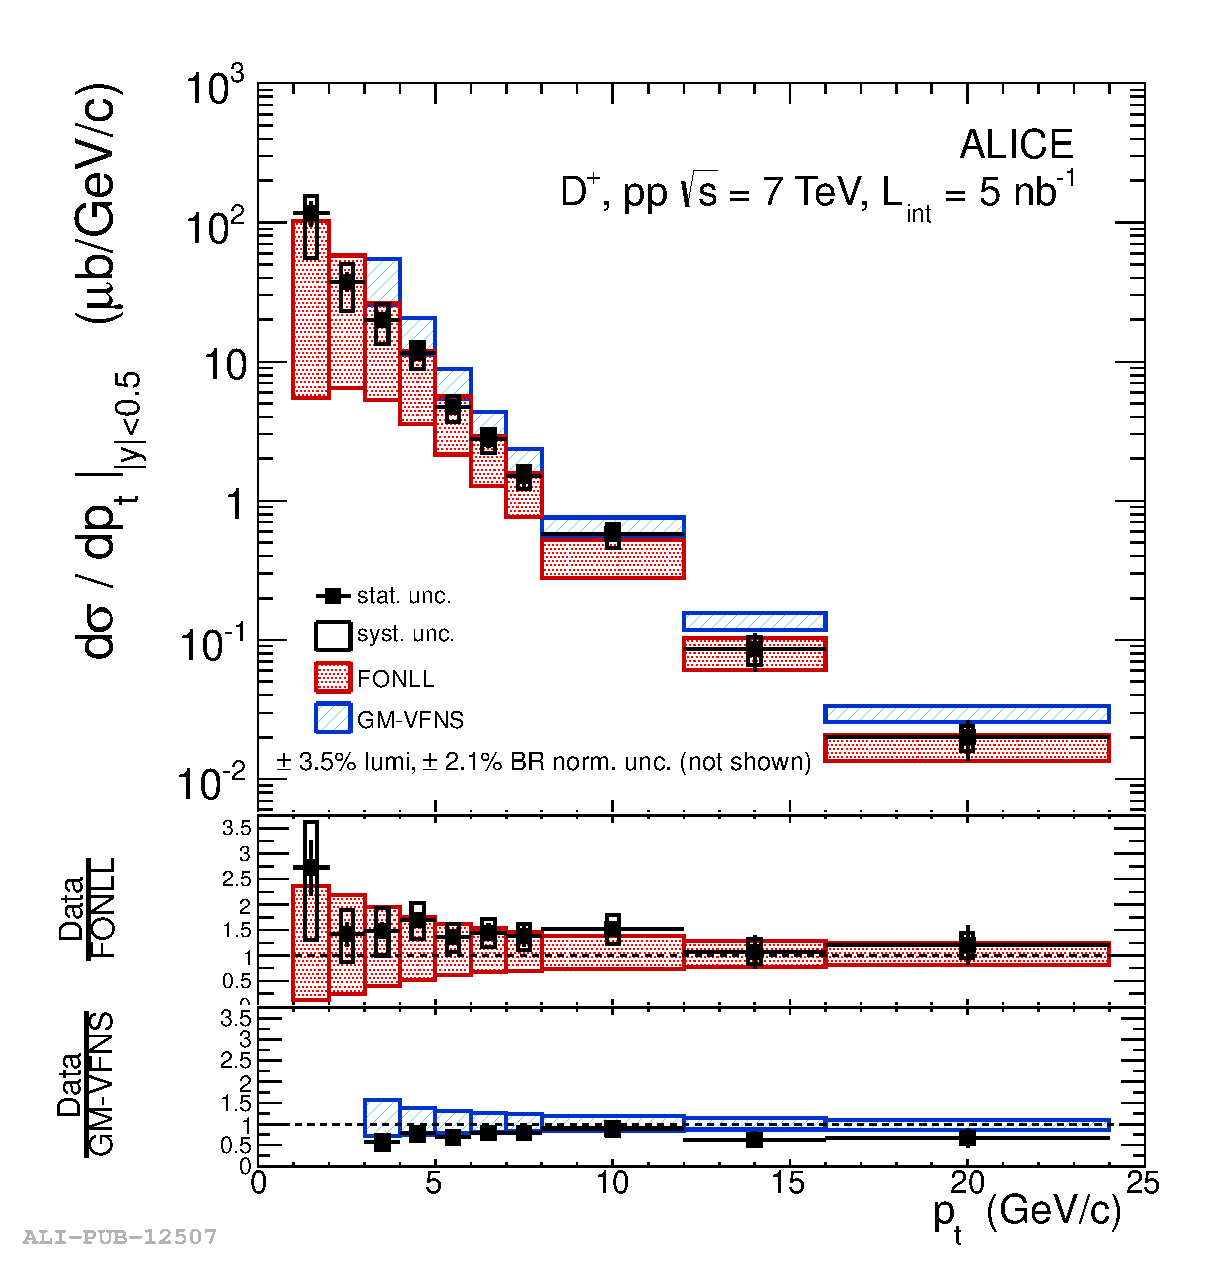
\includegraphics[scale = 0.3]{2012-Jun-06-DplusCrossSection_pp7TeV.eps}}
\hspace{0cm}
{\includegraphics[scale = 0.3]{jpsi_nonprompt_LHCb.png}}
\caption{Left: $\pt$-differential cross section for prompt $D^+$-meson production measured by ALICE in pp collisions at $\sqrt{s} = 7$ TeV compared with the FONLL and GM-VFNS calculations \cite{ALICE:2011aa}. Right: The non-prompt $J/\psi$ $\pt$-differential cross section measured by LHCb in pp collisions at $\sqrt{s} =$ 7 TeV compared to $J/\psi$ from $b$ production as predicted by FONLL \cite{Aaij:2011jh}.}
\label{HF_pp}
\end{center}
\end{figure}
\\\\
The fragmentation function describes the probability of hadronisation of the quark $q$ into the hadron $H$, which carry a fraction of
momentum of the quark $z_q = p_H/p_q$. As well as the PDFs, also the fragmentation functions are obtained from the experiment, in particular in $e^+e^-$ collisions, in which all the process before the hadronisation is perturbative, and therefore precisely calculated. Also for the fragmentation function case the evolution with $Q^2$ is evaluated with the DGLAP equations. These calculations describe well the experimental data, especially for the beauty hadrons. An example is the measurement of the cross section of $J/\psi$ from $b$ decays (non-prompt $J/\psi$) in pp collisions at $\sqrt{s} =$ 7 TeV performed by LHCb \cite{Aaij:2011jh}. In the right panel of figure \ref{HF_pp} it is possible to see the comparison of the data with the pQCD prediction (FONLL).
For the charmed hadrons the experimental results are also in agreement with the FONLL prediction, however all the measurements performed at Tevatron, RHIC and LHC show that the data are systematically on the upper edge of the theoretical prediction. An example of this behaviour is the $\pt$-differential cross section of prompt D$^+$-mesons (D$^+$ mesons coming directly from the hadronisation of a $c$-quark) measured in pp collisions at $\sqrt{s} =$ 7 TeV by ALICE \cite{ALICE:2011aa} (left panel of figure \ref{HF_pp}).
\section{Heavy-quark production in p-A and A-A collisions}
In heavy-ion collisions the production mechanism of heavy quarks is the same as in proton-proton collisions, since they are predominantly created in hard partonic scatterings, because of their large mass, in fact the thermal production in the QGP is negligible at the temperatures reached at RHIC and LHC. Therefore, neglecting medium effects, the hard particles production in heavy-ion collisions is expected to scale with the number of binary collisions, as explained in \ref{jet_sec}.
However, as for the high-$\pt$ hadrons, considering the $\pt$ spectrum, the binary scaling is broken by the interactions with the nuclear matter, which can be divided in two main categories:
\begin{itemize}
 \item Cold Nuclear Matter (CNM) effects 
 \item Hot Medium effects
\end{itemize}
The first category includes all the initial and final state effects which are not related to the formation of the QGP, but only to the presence of the nuclear matter, such as the modification of the PDFs in the nuclei with respect to free nucleons. On the contrary, the hot medium effects are related to the interaction with the deconfined medium, therefore they can be only final state effects. 
These modifications can be investigated and quantified with the nuclear modification factor, which was already defined in section \ref{jet_sec}. Here I report two different definitions, for A-A and p-A collisions, which are equivalent to the one in equation \ref{RAA}.
In case of nucleus-nucleus collisions the $R_{AA}$ can be expressed with the following formula: 
\begin{equation}
 R_{AA} = \frac{1}{\langle T_{AA} \rangle} \frac{dN_{AA}/d\pt}{d\sigma_{pp}/dpt},
 \label{RAA_HF}
\end{equation}
where $dN_{AA}/d\pt$ is the $\pt$-differential corrected yield measured in $A-A$ collisions, $\langle T_{AA} \rangle$ the average nuclear overlap function and $d\sigma_{pp}/d\pt$ the $\pt$-differential cross section measured in pp collisions. The same quantity, computed for p-A collisions can be written as
\begin{equation}
 R_{pA} = \frac{1}{\langle T_{pA} \rangle} \frac{dN_{pA}/d\pt}{d\sigma_{pp}/d\pt} = \frac{1}{A} \frac{d\sigma_{pA}/d\pt}{d\sigma_{pp}/d\pt},
 \label{RpA_HF}
\end{equation}
where $\sigma_{pA}/dpt$ is the $\pt$-differential cross section measured in p-A collisions and $A$ the mass number of the colliding nuclei. If there are no modifications due to initial or final state effects then, because of the binary scaling, we should observe a nuclear modification factor equal to 1 in the full $\pt$ range, otherwise it should be different. In particular, the various effects lead to different modifications in different $\pt$ regions, as explained in the following sections.
\subsection{Cold Nuclear Matter effects}
\label{CNM_sec}
In this section I will provide a brief explanation of initial-state CNM effects, which include the nuclear modification of the PDFs, the \textit{Cronin enhancement} and the initial-state energy loss in Cold Nuclear Matter (the energy-loss mechanism will be described in the following section, since is the same for heavy quarks travelling through the QGP). However, experimental observations might suggest also the presence of final-state effects in p-Pb collisions at LHC, due to the interaction of the produced heavy-flavoured hadrons with the particles produced in the collision, for which some kind of collective behaviour could be established.  
\subsubsection{Nuclear modification of the Parton Distribution Functions}
\begin{figure}[tb]
\begin{center}
\includegraphics[scale = 0.22]{PDF_nuclear_2.png}
\caption{Measurements of the nuclear modification of the PDFs performed by several experiments in a wide range of Bjorken $x$.}
\end{center}
\label{nPDFs}
\end{figure}
If the nucleus were a simple collection of almost free nucleons, the only modification expected for the PDFs would be due to the Fermi motion of the protons and neutrons inside the nucleus, which leads to a modification of the distribution of the fraction of the nucleon momentum $x$ carried by the partons. However, as observed for the first time by the European Muon Collaboration (EMC) in 1982 in muon-nuclei Deep Inelastic Scatterings experiments, there are other effects that should be taken into account. In order to quantify the modifications of the PDFs in bound nucleons it is possible to compute the ratio between the DIS cross section measured in experiments involving nuclei and the one with protons (or deuterium), normalised by the mass number A of the nucleus. This ratio can be equivalently expressed using the structure functions $F_2(x,Q^2)$, instead of the cross sections $\sigma_{DIS} (x,Q^2)$ 
\begin{equation}
 R^{A}(x,Q^2) = \frac{\sigma_{DIS}^A(x,Q^2)}{A\sigma_{DIS}^{nucleon}(x,Q^2)} = \frac{F_2^A(x,Q^2)}{AF_2^{nucleon}(x,Q^2)}
\end{equation}
This quantity has been measured by many experiments for several nuclei and different intervals of \textit{Bjorken} $x$. As shown in figure \ref{nPDFs} it is possible to distinguish four different regions of $x$:
\begin{itemize}
 \item For $x\lesssim 0.1$ a significant suppression is observed, which increases with the mass number of the nucleus. This interval is called \textit{shadowing region} \cite{Armesto:2006ph}. This effect can be explained by a phenomenological model (\textit{Color Glass Condensate}), which predicts a saturation of the partonic density at very low $x$, which leads to gluon fusion processes.    
\item The interval $0.1 \lesssim x \lesssim 0.3$ identifies \textit{the anti-shadowing region} where the ratio is slightly above the unity. 
 \item For $0.3 \lesssim x \lesssim 0.8$ the ratio is lower than unity, reaching a minimum around $x\simeq 0.7$. This suppression is called \textit{EMC effect} \cite{Rith:2014tma}.
 \item For $0.8 \lesssim x\lesssim 1$ the ratio is above unity because of the Fermi motion. 
\end{itemize}
Both the EMC effect and the shadowing increase with the mass number A or the density of the nucleus considered, while they almost do not show any dependence from the transferred momentum $Q^2$.\\ 
This modification affects the charm and bottom production in collisions involving nuclei, as it can be easily deduced from the factorisation theorem (see equation \ref{HF_prod_eq}). In particular, at LHC energies, the heavy-flavour production is expected to be influenced mostly by the shadowing, since, at central rapidity, $c\bar{c}$ and $b\bar{b}$ pairs are produced in hard scatterings with values of Bjorken $x$ around $\sim 10^{-4}$ for charm and $\sim 10^{-3}$ for beauty, increasing at high transverse momentum \cite{Carrer:2003ac}.
\subsubsection{Cronin enhancement}
The \textit{Cronin enhancement}, which was observed for the first time in p-A experiments at Fermilab \cite{Antreasyan:1978cw}, consists in an increase of the nuclear modification factor above unity, due to a shift of the $\pt$-spectrum toward higher values of transverse momentum. The interpretation of this effect is based on the idea that the partons inside the projectile particle go through multiple elastic collisions with the constituents of the target nucleus (\textit{random walk}), before the hard scattering. These elastic interactions transfer an initial transverse momentum $k_T$ to the partons, which is responsible of the $\pt$-spectrum shift for the particles produced in hard scatterings, such as heavy-quarks. 
\subsubsection{Nuclear modification factor in p-A collisions}
\label{RpPb_sec}
\begin{figure}[tb]
\begin{center}
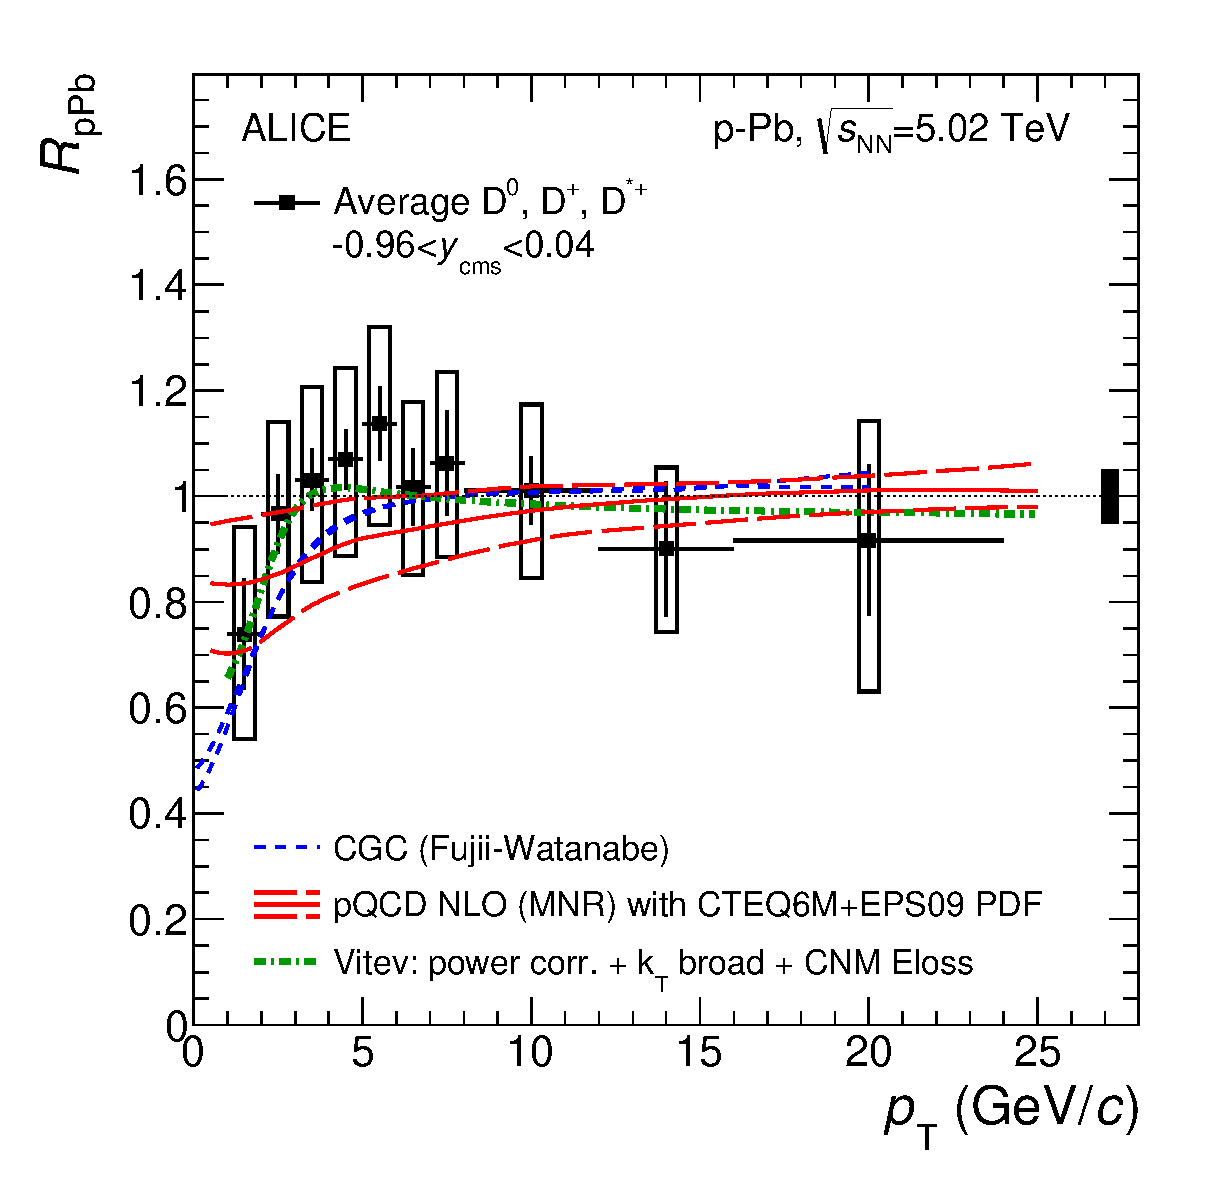
\includegraphics[scale = 0.3]{pPbWithModels.eps}
\hspace{0.cm}
{\includegraphics[scale = 0.3]{nonpromptJpsi_RpPb_LHCb.png}}
\caption{Left: nuclear modification factor $R_{pPb}$ for prompt D-mesons (average of D$^0$, D$^+$ and D$^{+*}$ as a function of the transverse momentum measured with the ALICE detector in p-Pb collisions at $\sqrt{s_{NN}} =$ 5.02 TeV compared to model calculations \cite{Abelev:2014hha}. Right: $\pt$-integrated nuclear modification factor $R_{pPb}$ for non-prompt $J/\psi$ as a function of rapidity measured by LHCb in p-Pb collisions at $\sqrt{s_{NN}} =$ 5.02 TeV \cite{Aaij:2013zxa}.}
\label{RpPb}
\end{center}
\end{figure}
Since the QGP formation is not expected in proton-nucleus collisions, their study is important to disentangle the effects of Quark-Gluon Plasma from those due to Cold Nuclear Matter, and to provide essential input to the understanding of the modifications observed in nucleus-nucleus collisions. An example of measurement in p-A collisions is shown in the left panel of figure \ref{RpPb}. The nuclear modification factor of D-mesons in the rapidity range $-0.96< y_{cms}<0.04$ measured in p-Pb collisions at $\sqrt{s_{NN}} =$ 5.02 TeV by the ALICE experiment \cite{Abelev:2014hha} can give a hint of an enhancement in the $\pt$ interval between 3 and 6 GeV/c, which can be attributed to the Cronin effect. However the effect is small and the experimental data are compatible with unity within the uncertainties.
The measurement is well reproduced by predictions which consider only initial-state effect, based either on next-to-leading order (NLO) pQCD calculations \cite{Mangano:1991jk} including the EPS09 modification of the CTEQ6M PDFs \cite{Eskola:2009uj}, or on the Color Glass Condensate \cite{Stump:2003yu}. Also calculations which include Cold Nuclear Matter energy loss, nuclear shadowing and $k_T$-broadening describe well the data \cite{Fujii:2013yja}. Another interesting measurement is the $\pt$-integrated $R_{pPb}$ for $J/\psi$ coming from B-hadrons decays as a function of rapidity \cite{Aaij:2013zxa}, performed by LHCb (right panel of figure \ref{RpPb}). In this case the experimental data are compatible with unity at backward rapidity (Pb-going direction), while they show a modest suppression at forward rapidity (p-going direction). This measurement is well described by NLO pQCD calculations with the EPS09 modification of the PDFs as shown in the figure. The suppression in the p-going direction is explained with the shadowing effect, since at forward rapidity smaller values of $x$ in the Pb nucleus are probed.
In both cases the results show that the Cold Nuclear Matter effects are small, especially at high transverse momentum.  
\subsection{Hot Medium effects}
As described in section \ref{HF_prod_sec}, because of their large mass, heavy quarks are exclusively produced via hard scatterings and therefore, according to the Heisenberg's uncertainty principle, they are created in the initial phase of the collision, before the QGP formation:
\begin{equation}
 \tau_{prod} \sim \frac{\hbar}{m_{b,c}} \sim 0.05 - 0.1\text{ fm/c}.
\end{equation}
Hence they subsequently interact with the constituents of the deconfined medium, and the modification of their dynamical properties is a powerful tool to investigate the Quark-Gluon Plasma. 
\subsubsection{In-medium energy loss}
\label{HF_AA}
Heavy quarks traversing a deconfined medium lose energy via elastic scatterings with the partons of the medium (\textit{collisional energy loss}) and gluon radiation (\textit{Gluonsstrahlung}). The first mechanism is similar to the ionisation energy loss of charged particles in ordinary matter via electromagnetic interaction, while the second one is the analogous in QCD of the QED \textit{Bremsstrahlung}. For a high energy parton the dominant mechanism is expected to be the gluon radiation, which can be described by the so-called BDMPS model \cite{Baier:1996sk}. According to this theoretical model, the mean energy loss 
\begin{equation}
 \langle \Delta E \rangle \propto \alpha_s C_R \hat{q} L^2
\end{equation}
is proportional to the square of the distance L traversed in the medium, to the strong coupling constant $\alpha_s$, to the colour coupling factor $C_R$ (which is equal to 3 for gluons and equal to 4/3 for quarks) and to a parameter $\hat{q}$ called transport coefficient, which depends on the gluon density (and therefore the energy density) of the medium. Moreover the \textit{dead cone effect} \cite{Djordjevic:2003qk} predicts that the energy loss decreases with increasing mass of the travelling parton, since the gluon emission is forbidden at angles smaller than 
\begin{equation}
\theta_c = M_q/E_q,
\end{equation}
where $M_q$ and $E_q$ are respectively the mass and the energy of the quark.
\subsubsection{Heavy-quark thermalisation}
The thermalisation of light quarks in the QGP is reached via multiple scatterings after a time of about $0.6-1$ fm/c at RHIC energies and even earlier at LHC. On the contrary, the thermal equilibrium of heavy quarks needs a longer time to be established, due to their larger mass, and eventually it can also not be reached. In particular, it is  more likely expected to be reached for charm and beauty quarks with low transverse momentum, since they have to lose less energy in the medium to thermalise. If the thermal equilibrium is completely reached, then the heavy quarks are subject to the same pressure gradients which act on light quarks, as explained in \ref{flows_sec}. Concerning that, the nuclear modification factor at low $\pt$ is a sensitive observable for the radial flow and can be an interesting tool to investigate the thermalisation of heavy quarks.
\subsubsection{Hadronisation via coalescence}
The heavy quarks which are produced in the core of the fireball could not have sufficient energy to emerge from the medium before hadronising. In this case, they can hadronise through a different mechanism, called \textit{coalescence}, which basically consists in the recombination with a light quark of the medium to form a heavy-flavoured hadron. The main difference of this mechanism with respect to the fragmentation described in section \ref{HF_prod_sec} is that, in this case, two low momentum partons form a higher momentum hadron, while in the fragmentation the final hadron has a fraction of the initial parton momentum $z_q=p_H/p_q$. In particular, it happens when two partons are close in the phase space and therefore have a significant overlap of their wave functions. The recombination picture becomes even more important in the presence of a thermalised medium, in which collective motions increase the probability to find a light quark close in space and with similar momentum with respect to the heavy quark. This alternative hadronisation method modifies the probability for the heavy quark to hadronise into a specific hadron $H$ and therefore the production mechanism of charmed and beauty hadrons.
\subsubsection{Nuclear modification factor in A-A collisions}
\begin{figure}[tb]
\begin{center}
\includegraphics[scale = 0.3]{AverageDmesonRaa_010_DzeroSTAR_010.png}
\hspace{0.cm}
{\includegraphics[scale = 0.283]{figures_PbPb_nonPromptJpsiCMS_wNpart.png}}
\caption{Left: prompt D-meson (average of D$^0$, D$^+$ and D$^{*+}$) nuclear modification factor as a function of $\pt$ in the 10\% most central Pb-Pb collisions measured by ALICE at $\sqrt{s_{NN}} = $ 2.76 TeV compared to D$^0$ $R_{AA}$ measured by STAR in Au-Au collisions at $\sqrt{s_{NN}} = $ 200 GeV \cite{Adam:2015sza}. Right: prompt D-meson $R_{AA}$ as a function of the number of participants measured by ALICE compared to $R_{AA}$ of non-prompt $J/\psi$ measured by CMS in Pb-Pb collisions at $\sqrt{s_{NN}} = $ 2.76 TeV \cite{Rossi:2014gma}.}
\label{RPbPb}
\end{center}
\end{figure}
The nuclear modification factor is an observable sensitive to the energy-loss mechanism, the radial flow and the shadowing effect which occur in A-A collisions. For example the left panel of figure \ref{RPbPb} shows the prompt D-meson $R_{AA}$ (average of D$^0$, D$^+$ and D$^{*+}$) as a function of $\pt$ in the 10\% most central Pb-Pb collisions at $\sqrt{s_{NN}} = $ 2.76 TeV measured by ALICE \cite{Adam:2015sza} together with the STAR measurement for D$^0$ mesons in central Au-Au collisions at $\sqrt{s_{NN}} = $ 200 GeV \cite{Adamczyk:2014uip}. For $\pt > 2-3$ GeV/c the two measurements are compatible within uncertainties and show a large suppression. On the contrary at low transverse momentum the STAR measurement shows a bump-like structure, which is less evident at LHC energies. This behaviour could be explained by the combination of radial flow and hadronisation via recombination described in the previous paragraphs. Note, also, that the initial-state effects presented in section \ref{CNM_sec}, and in particular shadowing, are different at the two collision energies. In the right panel of the same figure the D-meson $R_{AA}$ measured by ALICE for $8<pt<16$ GeV/c as a function of centrality expressed in terms of number of participants is compared with the nuclear modification factor of non-prompt $J/\psi$ with $\pt>6.5$ GeV/c measured at the same centre-of-mass energy by CMS \cite{Rossi:2014gma}. These results indicate a stronger suppression of charm hadrons than beauty hadrons in central Pb-Pb collisions, as expected from the predicted quark-mass dependence of energy loss discussed in the previous section.
\chapter{A Large Ion Collider Experiment}
\section{The Large Hadron Collider}
The Large Hadron Collider (LHC) is a two-ring superconducting hadron accelerator and collider based at the European particle physics laboratory CERN \cite{Evans:2008zzb}, near Geneva in Switzerland. The LHC is the world largest circular particle accelerator with a 26.7 kilometer circumference housed in a 3.8-meter-wide tunnel buried 50 to 175 meters underground.
It was constructed to accelerate mainly protons and Pb ions, which have to be pre-accelerated by smaller accelerators before to be injected in the LHC. In figure \ref{accelerators} it is possible to see a schematical representation of the full accelerator complex at CERN. \\Protons, obtained from hydrogen atoms, begin the chain in the Linear Accelerator 2 (LINAC2), where they reach an energy of 50 MeV. Subsequently, they are injected in the Proton Synchrotron Booster (PS Booster), which accelerate them to 1.4 GeV, then to the Proton Synchrotron, where they are accelerated up to 25 GeV. Finally they are sent to the Super Proton Synchrotron
(SPS), where they are accelerated to 450 GeV, and then they are ready to be injected into the LHC, where they reach their final energy.
The LHC proton collision design luminosity is $\mathcal{L} = 10^{34}$ cm$^{-2}$ s$^{-1}$ at a centre-of-mass energy of $\sqrt{s} =$ 14 TeV. The values of the centre-of-mass energy provided until now are 5.02, 7, 8 and 14 TeV. 
\begin{figure}[tb]
\begin{center}
\includegraphics[scale = 0.3]{accelerators.jpg}
\caption{Accelerator complex at CERN.}
\label{accelerators}
\end{center}
\end{figure}
Pb ions follow a different path. First electrons are stripped from lead into $^{208}_{82}$Pb$^{29+}$ ions and accelerated in the Linear Accelerator 3 (LINAC3) to an energy of 4.2 MeV per nucleon. Subsequently, Pb ions are further ionised (up to 54+) passing through a carbon foil. Then, they are accelerated into the Low Energy Ion Ring (LEIR), where they reach the energy of 72 MeV per nucleon, and then they enter into the PS which accelerate them up to 5.9 GeV. The final step before injecting the ions into the LHC is again the SPS, where the ions reach 177 GeV and get fully ionised with a second foil.     
The Pb-Pb collision design luminosity is $\mathcal{L} = 10^{27}$ cm$^{-2}$ s$^{-1}$ at a centre-of-mass energy per nucleon of $\sqrt{s_{\rm NN}} =$ 5.52 TeV, while the energies studied until now are 2.76 and 5.02 TeV.
The LHC provides the beams for the four largest experiments at CERN, which are placed on four of the eight beam intersections, as illustrated in figure \ref{accelerators}. They are:
\begin{itemize}
 \item A Large Ion Collider Experiment (ALICE): A detector designed to study the physics of strongly interacting matter at extreme energy densities, such as those reached in Pb-Pb collisions, where the formation of a new phase of matter, the Quark-Gluon Plasma (chapter \ref{QGP-section}), is expected. ALICE is also studying proton-proton and proton-Pb collisions as a comparison with Pb-Pb collisions.
 \item Compact Muon Solenoid (CMS): multi-purpose particle detector studying a wide range of physics, including the Higgs boson and the search for supersymmetry and dark matter.
 \item A Toroidal LHC Apparatus (ATLAS): multi-purpose experiment as CMS, but with complementary detection techniques.
 \item LHC beauty (LHCb): experiment designed to investigate the physics of beauty quark, especially the CP violation in the B-meson sector, and to study the matter-antimatter asymmetry.
\end{itemize}
\section{The ALICE detector}
\begin{figure}[tb]
\begin{center}
\includegraphics[scale = 0.45]{2012-Aug-02-ALICE_3D_v0_with_Text.jpg}
\caption{The ALICE schematic layout.}
\label{ALICE}
\end{center}
\end{figure}
ALICE is a general-purpose detector for the study of ultra-relativistic heavy-ion collisions \cite{Aamodt:2008zz}. It is designed to address the physics of strongly interacting matter and the QGP at extreme values of energy density and temperature. The physics programme includes not only Pb-Pb collisions, but also p-Pb collisions, in order to study Cold Nuclear Matter effects, and proton-proton collisions to provide a reference data for the heavy-ion programme. The ALICE detector can reconstruct charged particles down to
very low momenta (about 100 MeV/c for pions) in an environment characterised by a large charged particle multiplicity. In addition, a key feature of ALICE is the possibility to identify particles in a wide momentum range, using the information provided by different particle identification detectors.\\
Before to describe the ALICE apparatus, it is necessary to introduce the coordinate system used in the ALICE experiment, which is a right-handed Cartesian system. The $z$ axis identifies the beam direction, pointing to the ATLAS experiment (see figure \ref{accelerators}), while the orthogonal plane is defined by the $x$ and $y$ coordinates. In particular the $x$ axis is alligned with the horizontal and points toward the accelerator centre, while the $y$ axis is oriented upward. Furthermore, the polar angle $\theta$ is defined with respect to the $z$ direction and $\phi$, the azimuthal angle, increases counter-clockwise starting from the $x$ axis towards the CMS side.
The ALICE detector (figure \ref{ALICE}) is 26 m long, 16 m high, 16 m wide and weights more than 10000 tons. It consists of a central barrel part, which reconstructs hadrons, electrons and photons, and a forward muon spectrometer. The central part covers polar angles from 45\textdegree \space to 135\textdegree \space (which in terms of pseudorapidity means $|\eta| < 0.9$). It is embedded in a large solenoid magnet reused from the L3 experiment at LEP, which generates a magnetic field of B = 0.5 T parallel to the beam direction. From the inside out, the central barrel composed of the Inner Tracking System (ITS), which is made of two silicon pixel detector layers (SPD), two silicon drift detector layers (SDD) and two silicon strip detector layers (SSD), a large cylindrical Time Projection Chamber (TPC), the Transition Radiation Detector (TRD), the Time Of Flight (TOF) detector, the Ring Imaging Cherenkov (HMPID) detector, and two electromagnetic calorimeters (PHOS and EMCal). All these detectors cover the full azimuth, except for PHOS, HMPID and EMCal.\\
The forward muon arm covers polar angles from 2\textdegree \space to 9\textdegree \space(which in terms of pseudorapidity means $-4 < \eta < -2.5$) and the full azimuth. It consists of a complex arrangement of absorbers, a large dipole magnet and fourteen planes of tracking and triggering Resistive Plate Chambers (RPC).\\
ALICE includes also several smaller detectors for global event characterisation and triggering (ZDC, PMD, FMD, T0, V0A and V0C) and an array of scintillators (ACORDE) located on top of L3 magnet used to trigger on cosmic rays.
In the next sections the more detailed description of the main sub-detectors used in the analysis presented in this thesis is provided.
\subsection{Inner Tracking System (ITS)}
\label{ITS_sec}
The ITS \cite{Nooren:2007zz} is the first sub-detector reached by the particles originating from the collisions. The main tasks of this detector are:
\begin{itemize}
\item The localisation of the primary vertex with a resolution better than 100 $\mu$m.
\item The reconstruction of the secondary vertices from the decays of D and B mesons and hyperons.
\item The tracking and identification of the particles with momentum below 200 MeV/c. 
\item The improvement of the momentum and the angle resolution for particles reconstructed by the TPC.
\end{itemize}
Because of the high particle density in heavy-ion collisions, and in order to achieve the required impact-parameter (distance of closest approach between the tracks and the primary vertex) resolution, Silicon Pixel Detectors (SPD), which has a spatial resolution of about 12 (100) $\mu$m in the $r\varphi$ ($z$) direction, have been chosen for the innermost two layers, Silicon Drift Detectors (SDD) for the following two layers and Silicon Strip Detectors (SSD) for the last two layers. The four outer layers have analogue readout and therefore can be used for Particle IDentification (PID) via $dE/dx$ measurement. 
The dimensions of each sub-detector are summarised in table \ref{ITStable}. Since the momentum and impact-parameter resolutions for low-momentum particles are dominated by multiple scattering effects in the detector material, the amount of material in the active volume has been minimised, resulting to an amount of single detector effective thickness of about 0.4\% of X$_0$. The total material encountered, including the support structures and the shields, by a perpendicular track crossing the ITS is around 7.2\% of X$_0$.
\subsubsection{Silicon Pixel Detectors (SPD)}
\begin{figure}[tb]
\begin{center}
\includegraphics[scale = 0.5]{its.png}
\caption{Layout of the Inner Tracking System.}
\label{ITS}
\end{center}
\end{figure}
The Silicon Pixel Detector is a fundamental element for the determination of the position of the primary vertex as well as for the measurement of the impact parameter of secondary tracks originating from the weak decays of strange, charm and beauty particles. Thanks to its fast response, it can also provide a fast trigger signal.
The SPD is based on hybrid silicon pixels, consisting of a two-dimensional matrix (sensor ladder) of reverse-biased silicon detector diodes bump-bonded to the readout chips. The readout is binary, which means that the digital output changes when the signal is above a set threshold.
The sensor matrix includes 256 x 160 cells, corresponding to a sensor area of 12.8 mm ($r\varphi$) x 70.7 mm ($z$). 
The thickness of the sensor is 200 $\mu$m which is the smallest that can be achieved with an affordable yield in standard processes.
In total the SPD has 240 ladders and 1200 readout chips, for a total of 9.8 10$^6$ cells. It has an intrinsic spatial resolution of about 12 $\mu$m in $r\varphi$ direction and 100 $\mu$m in $z$ direction, and a two-track resolution of about 100 $\mu$m in $r\varphi$ direction and 850 $\mu$m in $z$ direction. 
\begin{table}[tb]
\centering 
\begin{center} % 
\renewcommand\arraystretch{1.19} 
\begin{tabular}{|c|c|c|c|c|c|}
\hline
Layer & Sub-detector & r (cm) & z (cm) & Active Area (m$^2$) & Channels\\
\hline
1 & SPD & 3.9 & 14.1 & 0.07 & 3276800\\
2 & SPD & 7.6 & 14.1 & 0.14 & 6553000\\
3 & SDD & 15.0 & 22.2 & 0.042 & 43008\\
4 & SDD & 23.9 & 29.7 & 0.89 & 90112\\
5 & SSD & 38.0 & 43.1 & 2.20 & 1148928\\
6 & SSD & 43.0 & 48.9 & 2.80 & 1459200\\
\hline
\end{tabular}
\caption{Dimensions of the Inner Tracking System.}
\label{ITStable}
\end{center} 
\end{table}
\subsubsection{Silicon Drift Detectors (SDD)}
The ALICE Silicon Drift Detectors have very good multi-track capability and provide two out of the four $dE/dx$ samples needed for the ITS particle identification. The sensors were produced from a very homogeneous high-resistivity (3 k$\ohm$cm) Neutron Transmutation Doped (NTD) silicon. They have a thickness of 300 $\mu$m and a sensitive area of 70.17 mm ($r\varphi$) x 75.26 mm ($z$), which is split into two drift regions by the central cathode strip to which a bias of 1.8 kV is applied. In each drift region on both detector surface there are 291 cathode strips, with 120 $\mu$m pitch, which completely deplete the detector volume and generate a drift field of about 500 V/m parallel to the surface. Each drift region has 256 anodes with 294 $\mu$m pitch, where the electrons generated by the crossing charged particles are collected. The layout of a sensor is shown in figure \ref{SDD}. The $r\varphi$ coordinate of the crossing particle is obtained from the drift time of the electrons with respect to the trigger time. The drift speed depends on temperature ($v_{drift} \propto T^{-2.4}$), therefore for each drift region there are 33 MOS charge injectors to monitor the drift velocity during data acquisition.\\
The space precision of the SDD is better than 38 $\mu$m in $r\varphi$ direction and 25 $\mu$m in $z$ direction (it grow up to 60 $\mu$m close to the anodes).The double-track resolution is estimated to be around 200 $\mu$m for $r\varphi$ direction and 600 $\mu$m for $z$ direction.  
\begin{figure}[tb]
\begin{center}
\includegraphics[scale = 0.25]{SDD.png}
\caption{Layout of a SDD sensor.}
\label{SDD}
\end{center}
\end{figure}
\subsubsection{Silicon Strip Detectors (SSD)}
The Silicon Strip Detector is crucial for the prolongation of tracks from the TPC to the ITS. SSDs also provide $dE/dx$ information to assist PID for low-momentum particles. 
The basic SSD module is a double-sided strip detector. The sensors are 300 $\mu$m thick and have 768 strips on each side with 95 $\mu$m pitch. The stereo angle between the strips of the two sides is 35 mrad, which is a compromise between the best resolution on $r\varphi$ direction and the minimisation of ambiguous measurement resulting from high particle densities.
The spatial resolution is about 20 $\mu$m in $r\varphi$ direction and 800 $\mu$m in $z$ direction. 
\subsection{Time Projection Chamber (TPC)}
The Time Projection Chamber \cite{Schmidt:2010zzc} is the main tracking detector of the central barrel and it is optimised to provide charged particle momentum measurements with good two-track separation and particle identification via $dE/dx$. In addition data from central barrel can be used to generate a fast online High-Level Trigger (HLT) for the selection of low cross section signals.\\
The TPC, as shown in figure \ref{TPC}, is cylindrical; it covers the full azimuthal angle, having an active radial range from about 85 cm to 250 cm and and overall length along the beam direction of 500 cm. It covers the pseudorapidity range $|\eta| < 0.9$ for tracks with full radial track length (matches in ITS, TRD and TOF), and up to $|\eta| = 1.5$ for reduced track length. The TPC also allows charged particle reconstruction in a wide range of transverse momentum, from low $\pt$ of about 0.1 GeV/c up to 100 GeV/c. Each end plate is divided in 18 trapezoidal sectors, where multi-wire proportional chambers are mounted. The field cage is based on a design with a central high-voltage electrode and two opposite axial resistive potential dividers, which create a highly uniform electrostatic field in the common gas volume.
The choice of the gas is strongly dependent on the requirements imposed by the extreme environment of Pb-Pb collisions. In fact the ALICE TPC has been designed for a maximum multiplicity $dN_{ch}/dy = 8000$, resulting in 20000 charged primary and secondary tracks in the acceptance, an unprecedented track density for a TPC. Therefore, the drift gas Ne/CO$_2$/N$_2$ was initially chosen and used during Run I data taking (2009-2013). This gas mixture is optimised for drift speed, low diffusion, low radiation length and hence low multiple scattering, small space-charge effect and ageing and stability effects. The N$_2$ mixture improves the quenching and allows higher maximum gas gains. 
\begin{figure}[tb]
\begin{center}
\includegraphics[scale = 0.4]{tpc.png}
\caption{Layout of the ALICE Time Projection Chamber.}
\label{TPC}
\end{center}
\end{figure}\\
Thanks to this design, the detector provides more than 90\% efficiency in track finding, with a resolution up to about 2\% in charge particle momentum measurement at $\pt \approx 10$ GeV/c. The relative $dE/dx$ resolution was measured to be 6\% for particle crossing the entire detector.
\subsection{Time of Flight (TOF)}
\label{TOFsec}
The Time of Flight detector \cite{Alici:2012fp} is a large area detector arranged around the TRD, it covers the same pseudorapidity range of ITS, TPC and TRD ($|\eta|< 0.9$). Its main purpose is the particle identification in the intermediate momentum range, up to 2.5 GeV/c for pion-kaon separation and up to 4 GeV/c for proton-kaon separation.\\
The TOF is made of Multi-gap Resistive Plate Chambers (MRPC) which cover an area of about 160 m$^2$ filled with a gas mixture
composed of 90\% of C$_2$ H$_2$ F$_4$, 5\% of C$_4$ H$_10$ and 5\% of SF$_6$. Each multi-gap is made of 10 layer double-stack strip detectors with a time resolution of about 40 ps. The time of flight for each particle is given together with the information of the start time of the event, $t_0$ ($t_{flight} = t_{hit}-t_0$). The start time $t_0$ is determined with the T0 detector or using the particle arrival times at the TOF. The overall TOF resolution is around 85 ps in Pb-Pb events and 100 ps in proton-proton collisions, where there is a larger uncertainty on the determination of the event time zero. \\
\section{ALICE trigger and data acquisition}
\subsection{Central Trigger Processor}
\label{MBtrigger_sec}
The ALICE Central Trigger Processor (CPT) \cite{ALICEtrigger} collects and manages all the trigger inputs coming from all the detectors and provides a trigger signal to the readout detectors in case of fulfilled trigger conditions. The main features of the CPT are the capability to combine many detectors, which are busy for widely different periods, and to perform optimised trigger selections for different running modes (Pb-Pb, p-Pb and pp), varying by almost two orders of magnitude in counting rate. The first level trigger signal, called L0 and made of 24 inputs, arrives 1.2 $\mu s$ after the collision. The signals from the detectors which are not fast enough for L0 trigger are collected in the level 1 trigger signal (24 L1 inputs), that is sent after 6.5 $\mu s$. Finally a third level of trigger (12 L2 inputs) is sent after 88 $\mu s$, which is the maximum drift time of electrons in the TPC, in order to guarantee a past-future protection that looks for other events of requested type in the time window around the collision under investigation. This feature helps the rejection of the pile-up events in the TPC.\\
The \textit{minimum-bias} (MB) trigger which will be used in the analysis presented in this thesis is the one used in p-Pb collisions, which requires the signal from both V0A and V0C detectors (see figure \ref{ALICE}).
\subsection{Data AcQuisition System and High-Level Trigger}
The Data AcQuisition (DAQ) system of ALICE must operate in really challenging conditions, starting from the high interaction in rate proton-proton collisions to the huge amount of data collected in Pb-Pb collisions (up to 4 Gb/s).\\
If all the trigger requirements are fulfilled, the data are sent to the Detector Data Link (DDL) and then to the Local Data Concentrators, a farm of computers which builds sub-events from the event fragments they receive from the front-end electronics. Finally, the complete event is built by the Global Data Collectors (GDC), which send it to the storage facilities if it is accepted by the High Level Trigger (HLT). The HLT can accept or reject an event after performing an online analysis, which includes a fast track and primary vertex reconstruction. Then, if the event is accepted, the High Level Trigger compress the data and transfer them to the CERN computer centre, where they are registered on tape.      
\section{ALICE performance}
\subsection{Track and vertex reconstruction in the central barrel}
\label{vertex_reco_sec}
In ALICE the tracking procedure starts with the conversion of the detector hits in \textit{clusters}, characterised by several quantities, such as position, signal amplitude and signal time, and their associated errors. Then, a first evaluation of the primary vertex is performed using the clusters in the two innermost layers of the ITS (SPD). It is determined as a space point to which a maximum number of tracklets (lines defined by pairs of clusters, one cluster in each SPD layer) converge (\textit{Vertexer3D}). In low multiplicity events, if it is not possible to find a single point of convergence, the algorithm performs a one-dimensional minimisation to reconstruct the position of the interaction point along the beam direction ($z$ axis) by using the distances of closest approach of the tracklets to the average position of the beam in the transverse plane (\textit{VertexerZ}). After this procedure the tracks are reconstructed and fitted in TPC and ITS using the Kalman Filter algorithm \cite{Fruhwirth:1987fm} and subsequently prolonged to the other central barrel detectors and fitted again. The procedure can be summarised in the following steps: 
\begin{itemize}
 \item The track seeds are build first from the clusters in the two outermost pad rows of the TPC and the primary vertex. Then, with three clusters and without the vertex constraint. Then, the seeds are propagated inward and updated with every nearest cluster found by the Kalman Filter algorithm, until the inner radius of the TPC is reached.
 \item The tracks reconstructed in the TPC are matched to the hits in the outermost SSD layer and become the seed for the track finding in the ITS. The seed is then propagated inward and updated at each ITS layer attached to all the clusters within a proximity cut. Therefore, for each TPC track, a corresponding tree of track hypotheses in the ITS is produced. The candidates are then selected according to their $\chi^2$. In the left panel of figure \ref{tracking} is shown the comparison between the fraction of tracks in TPC which have a prolongation in the ITS (\textit{matching efficiency}) in data and in the simulation for Pb-Pb collisions at $\sqrt{s_{NN}} =$ 2.76 TeV, for different requirements on ITS points \cite{Abelev:2014ffa}. 
 \item The hits in the ITS not attached to tracks propagated from the TPC are used to perform an ITS stand-alone reconstruction, which allows to obtain a better efficiency for tracks with low transverse momentum and to reconstruct tracks of particles traversing dead zones of the TPC or which decay before entering in the TPC. 
 \item The tracks obtained are then back-propagated in the outward direction in order to match the clusters in the TRD and TOF, and the signals in EMCal, PHOS and HMPID. Finally, the tracks are re-fitted inward using the previously found clusters. The parameters of the track state vector and its covariance matrix are calculated. 
\end{itemize}
\begin{figure}[tb]
\begin{center}
{\includegraphics[scale = 0.3]{06-tracking_ITS_TPC_trackingEff_PbPb.png}}
\hspace{0cm}
{\includegraphics[scale = 0.3]{06-tracking_d0rphi_res_pp_pPb_PbPb_dataonly.png}}
\caption{Left: comparison between the TPC-ITS matching efficiency, defined as the fraction of TPC tracks with a prolongation in the ITS, in data and in the simulation for Pb-Pb collisions at $\sqrt{s_{NN}} =$ 2.76 TeV, for different requirements on ITS points. Right: impact-parameter resolution in the $xy$-plane for primary particles in pp, p-Pb and Pb-Pb collisions.}
\label{tracking}
\end{center}
\end{figure} After this procedure, if it is possible, the primary vertex is re-evaluated using the reconstructed tracks. The determination of the primary vertex with the tracks instead of the SPD tracklets allows to improve significantly the resolution, which is fundamental for analysis of charm and beauty hadrons, whose decay vertices are typically displaced by hundreds of microns from the primary vertex.\\
The right panel of figure \ref{tracking} shows the resolution of the distance of closest approach to the primary vertex (impact parameter) in the transverse plane for charged tracks in pp, p-Pb and Pb-Pb collisions \cite{Abelev:2014ffa}. From this picture it is possible to notice that the resolution is slightly better in p-Pb and even more in Pb-Pb collisions as compared to pp interactions, because the reconstruction on the primary vertex position improves with increasing multiplicity of charged particles produced in the collision.\\
The reconstructed data are stored in files containing all the physical information needed for the analysis and for checking the quality of the reconstruction for each sub-detector in a format called ESD (\textit{Event Summary Data}). In order to reduce the size of the files and the computational time needed for the analysis, the AOD (\textit{Analysis Object Data}) files, which contains only the information needed for the analysis, are produced. The conversion from ESD to AOD is called \textit{filtering}. In addition, the AODs also contain some initial step of the analysis. For example, for the D-meson analysis, the AODs already contain the D-meson candidates, which are combinations of tracks coming from a secondary vertex, selected with loose criteria.   
\subsection{Particle IDentification (PID)}
\label{PID_sec} 
One of the distinctive features of the ALICE detector is the excellent particle identification capability, which can be performed in a wide range of momentum, exploiting different techniques. In this section I only discuss the subsystem for identifying charged hadrons  used in the analysis described in this thesis, which are the Time Projection Chamber and the Time of Flight. 
\subsubsection{PID with the Time Projection Chamber}
The PID with the Time Projection Chamber is performed by simultaneously measuring the specific energy loss (via the measurement of the charge deposited on up to 159 pad rows), the charge and the momentum of each particle traversing the detector gas. A truncated mean of the $dE/dx$ is calculated using the 65\% of the lowest-amplitude clusters. The particle identification is based on the comparison of the measured $dE/dx$ and the expected $dE/dx$ for a specific particle species with a certain momentum $p$. The relative $dE/dx$ resolution achieved is about of the 6\% for particle crossing the entire detector. In the left panel of figure \ref{PID} is shown the specific energy loss measured with the TPC in p-Pb collisions as a function of the track momentum, with the Bethe-Bloch curves for electrons, pions, kaons, protons, deuterium and tritium superimposed.
The TPC provides a better particle identification for $\pt \lesssim$ 0.7 GeV/c, where the largest separation is achieved (see figure \ref{PID}), however in the relativistic rise region (2 $\lesssim \pt \lesssim$ 20 GeV/c) a statistical approach allows to extract the relative abundances.  
\subsubsection{PID with the Time of Flight}
\begin{figure}[tb]
\begin{center}
{\includegraphics[scale = 0.092]{2013-Oct-18-dEdx_pPb_zoom_logo.png}}
\hspace{0cm}
{\includegraphics[scale = 0.087]{2013-Mar-06-betap_v5.png}}
\caption{Left: specific energy loss ($dE/dx$) in the TPC as a function of the particle momentum in p-Pb collisions at $\sqrt{s_{NN}} =$ 5.02 TeV. The lines show the parametrisation of the expected mean energy loss. Right: velocity $\beta$ as measured with the TOF detector as a function of momentum for particles reaching the TOF in p-Pb collisions at $\sqrt{s_{NN}} =$ 5.02 TeV.}
\label{PID}
\end{center}
\end{figure}
The Time of Flight is a dedicated PID detector, which measures the arrival time of particles. In order to obtain the flight time of the particles the start time for the TOF detector can be provided either by the T0 detector, which consists of two arrays of Cherenkov counters (T0A and T0C), positioned at opposite sides of the interaction point (see figure \ref{ALICE}) or via a combinatorial analysis
of the particle  arrival times at the TOF detector. The overall TOF resolution, including the uncertainty on the start time of the event, and the tracking and momentum resolution contributions, is up to $\sim 85$ ps for high-multiplicity p-Pb collisions \cite{Abelev:2014ffa}. As shown in the right panel of figure \ref{PID}, where the particle velocity is plotted as a function of momentum, the TOF detector provides a good proton-kaon separation up to $\pt \simeq 4$ GeV, while for larger values it is not possible to achieve a satisfactory separation among the hadron species. 
\chapter{Prompt D$^+$-meson reconstruction strategy}
\label{Dplus_reco}
\begin{table}[b]
\centering 
%\par\medskip
\begin{center} % 
\renewcommand\arraystretch{1.19} 
\begin{tabular}{|c|c|c|c|c|}
\hline
Meson & Mass (MeV/c$^2$) & decay channel & BR(\%) & $c\tau$ ($\mu$m) \\
\hline
D$^+$ & 1869.61 $\pm$ 0.09 & K$^-\pi^+\pi^+$ & 9.13 $\pm$ 0.19 & 311.8\\
D$^0$ & 1865.84 $\pm$ 0.05 & K$^-\pi^+$ & 3.88 $\pm$ 0.05 & 122.9\\
D$^{*+}$ & 2010.27 $\pm$ 0.05 & D$^0\pi^+ \rightarrow$ K$^-\pi^+\pi^+$ & 67.7 $\pm$ 0.5 & strong decay\\
D$_s^+$ & 1969.30 $\pm$ 0.10 & $\phi\pi^+ \rightarrow$ K$^+$K$^-\pi^+$ & 2.24 $\pm$ 0.10 & 149.9\\
\hline
\end{tabular}
\caption{D-mesons hadronic decays measured by the ALICE Collaboration. The Characteristics reported are from \cite{Agashe:2014kda}.}
\label{Dmesons_tab}
\end{center} 
\end{table}
This Chapter is dedicated to the description of the strategy for the reconstruction of the D$^+$-mesons in p-Pb collisions at $\sqrt{s_{NN}} =$ 5.02 TeV, which is adopted for both the standard analysis published by the ALICE Collaboration \cite{Abelev:2014hha} and the analyses presented in this thesis. The D$^+$-mesons are reconstructed in the hadronic decay channel D$^+\rightarrow $ K$^-\pi^+\pi^+$, which has a branching ratio of 9.13\%, as reported in table \ref{Dmesons_tab}. D$^+$-mesons can be \textit{prompt}, if they come directly from the hadronisation of a $c$-quark or from the decay of a excited open charm or charmonimum state, or \textit{feed-down}, if they originate from the decay of hadrons containing $b$-quarks. In the first section of this Chapter both the contributions are considered as \textit{signal} against the \textit{background} due to combinatorial background, while starting from the second section the two contributions to the D$^+$ measured yield are treated separately. Most of the procedures described in the following sections were already implemented in the analysis framework of ALICE, however for the analysis presented in Chapter \ref{KF_chapter} I re-implemented them. This was done because of the different file format needed for the analysis: while the studies presented in Chapter \ref{IP_chapter} and \ref{CV_chapter} were performed on the AODs (see section \ref{vertex_reco_sec}), which already contain the information of the D$^+$ candidates, for the analysis in Chapter \ref{KF_chapter} the ESDs were needed because of the different vertexing package used.
\section{D$^+$ candidate reconstruction and selection}
\begin{figure}[tb]
\begin{center}
{\includegraphics[scale = 0.25]{Dplus_sketch.png}}
\caption{Sketch of the D$^+$ hadronic decay D$^+ \rightarrow$ K$^-\pi^+\pi^+$ and some of the reconstructed topological quantities associated.}
\label{Dplus_sketch}
\end{center}
\end{figure}
D$^+$-mesons (and their charge conjugates) are reconstructed in the hadronic decay channel D$^+$ $\rightarrow$ K$^{-} \pi^+ \pi^+$, using an analysis based on the selection of fully reconstructed decay topologies displaced from the primary interaction vertex. This is possible thanks to the relatively high branching ratio ($BR=$9.13\%) of this decay and the mean proper decay length of the D$^+$ ($c\tau=$312 $\mu$m), which allows one to resolve the decay vertex from the interaction vertex. The main D$^+$ $\rightarrow$ K$^{-} \pi^+ \pi^+$ characteristics are summarised in table \ref{Dmesons_tab}, together with the other D-mesons measured by ALICE for comparison. Even if the branching ratios were recently updated by the PDG (see \cite{Agashe:2015up}), I reported the values from \cite{Agashe:2014kda}, since the analyses which I will present are performed using these values in order to be able to compare the results with the published ones.
\subsection{p-Pb data sample and event selection}
\label{datasample}
The analysis is performed on a data sample of p-Pb collisions at $\sqrt{s_{NN}} =$ 5.02 TeV collected in 2013 with the ALICE detector. The events were selected online using a Minimum Bias trigger which requires signals in both V0 detectors, as explained in section \ref{MBtrigger_sec}. Furthermore, only the events which pass a selection, called \textit{physics selection}, based on the timing information of V0 and ZDC detectors are considered for the analysis. This selection removes background events due to the interaction of the beams with the residual gas molecules present in the vacuum tube. \\
As discussed in section \ref{vertex_reco_sec}, the interaction vertex can be reconstructed using global (ITS-TPC) tracks or only SPD tracklets. Considering that the D$^+$ decay length is of the order of hundred of microns, it is crucial to have a primary vertex reconstructed as precisely as possible. Therefore, only the vertices reconstructed with global tracks are kept into account. In order to have a uniform acceptance for tracks in the ITS and TPC detectors, all the events with the reconstructed primary vertex position along the beam direction ($z_{vtx}$) more than 10 cm away from the nominal interaction point position are rejected. Finally, the events with at least two reconstructed interaction vertices having a minimum distance of 0.8 cm between each other and the lower multiplicity vertex with minimum 5 contributors, are identified as pile-up events and rejected. This selection rejects less than 1\% of the events passing the physics selections, as expected for the interaction rate of the Minimum Bias p-Pb data taking, which was of about 10 kHz.
After all these selections the number of events available results to be of about 100 million, which corresponds to an integrated luminosity of about $L_{int} = N_{MB}/\sigma_{MB}^{pPb} =$ 48.6 $\mu \text{b}^{-1}$, where $\sigma_{MB}^{pPb}$ is the Minimum Bias cross section measured with van der Meer scans \cite{Abelev:2014epa} ($\sigma_{MB}^{pPb} = 2.09 \pm 3.5\%$ b).
\subsection{Track selection}
The D$^{+}$-meson candidates are built by combining three ITS-TPC tracks which fulfil several kinematical and quality requirements. First of all, only the tracks which have been successfully fitted by the Kalman filter algorithm during the final inward refit step described in section \ref{vertex_reco_sec} are selected. Then tracks are required to have at least 70 associated space points in the TPC (out of a maximum of 159) and 2 hits in the ITS (out of six possible), of which at least one has to be in one of the two SPD layers. This latter requirement is really important for the heavy-flavour measurements, since it provides optimal impact-parameter and secondary-vertex resolution, thanks to the presence of a measured point close to the primary and secondary vertices. Furthermore the tracks are selected by requiring a fit quality of $\chi^{2}/ndf < 2$ in the TPC. Finally only the tracks with $|\eta| <$ 0.8 and $\pt >$ 0.3 GeV/c are taken into account for the analysis.
\subsection{D$^+$ reconstruction in the fiducial acceptance region}
\begin{figure}[tb]
\begin{center}
{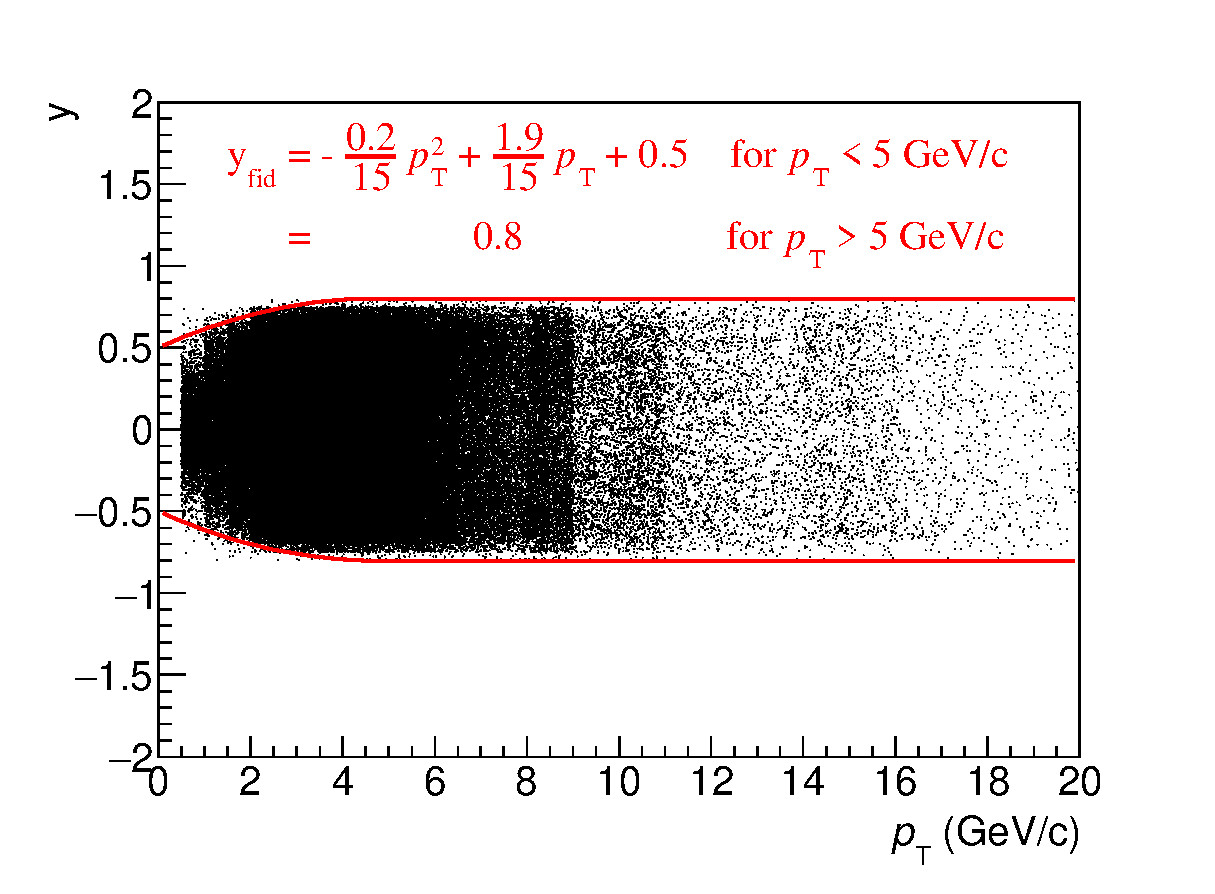
\includegraphics[scale = 0.4]{fiducialacc.eps}}
\caption{Rapidity vs transverse momentum distribution of the reconstructed D$^+$-mesons. The fiducial acceptance region is defined as $|y_{D+}| < y_{fid}(\pt)$.}
\label{fidacc}
\end{center}
\end{figure}
The D$^\pm$-meson candidates are reconstructed combining triplets of good tracks with the proper charge sign (two positive tracks and one negative track for the D$^+$ and the opposite for the D$^-$). For each candidate the momentum and the invariant mass are calculated starting from the energy and momentum of the measured tracks
\begin{equation}
\begin{cases}
\vec{p} = (p^x_K+p^x_{\pi_1}+p^x_{\pi_2},\text{ }p^y_K+p^y_{\pi_1}+p^y_{\pi_2},\text{ }p^z_K+p^z_{\pi_1}+p^z_{\pi_2})\\[3mm]
M_{K\pi\pi} = \sqrt{(E_K+E_{\pi_1}+E_{\pi_2})^2-(\vec{p}_K+\vec{p}_{\pi_1}+\vec{p}_{\pi_2})^2}
\end{cases}
\end{equation}
where
\begin{equation}
 E_{K,\pi} = \sqrt{m_{K,\pi}^2+\vec{p}_{K,\pi}^{\text{ }2}}.
\end{equation}
The mass of the kaon $m_K$ is assigned to the track with the opposite charge sign with respect to the D$^+$ candidate and the mass of the pion $m_\pi$ to the other two tracks. 
For each candidate the associated rapidity is calculated using the reconstructed quantities as
\begin{equation}
 y_{D^+} = ln\bigg{(}\frac{E+p_z}{E-p_z}\bigg{)},
\end{equation}
where $E$ is the energy of the candidate computed using its momentum component and the D$^+$ mass from the PDG. Only the D$^+$ mesons which are in a fiducial acceptance region are considered for the analysis. This is needed to exclude the $y$ regions where the acceptance steeply decreases due to the single track selections ($|\eta| <$ 0.8 and $\pt >$ 0.3 GeV/c). The fiducial acceptance region is $\pt$-dependent, since D$^+$-mesons with low transverse momentum have a lower acceptance, because of the larger dispersion of the daugher tracks around the D$^+$ flight direction. Therefore the rapidity values accepted are those within $|y_{D+}| < y_{fid}(\pt)$, where $y_{fid}(\pt)$ increases from 0.5 for $\pt = 0$ up to 0.8 for $\pt>5$ GeV/c, as shown in figure \ref{fidacc}.
\subsection{Topological selections}
\label{topocuts}
The D$^+$ candidates are dominated by the background because of the large number of track combinations. Therefore it is necessary to apply geometrical selections on the displaced decay vertex topology, in order to improve the signal over background ratio and the statistical significance of the signal. First of all, for this purpose, the decay vertex position is computed performing a minimisation of the distance among the tracks of the selected triplet, weighted according their uncertainties. Then other geometrical and kinematical quantities, which can discriminate the D$^+$ signal from the combinatorial background, are exploited.
\subsubsection{Decay length}
\begin{figure}[b]
\begin{center}
{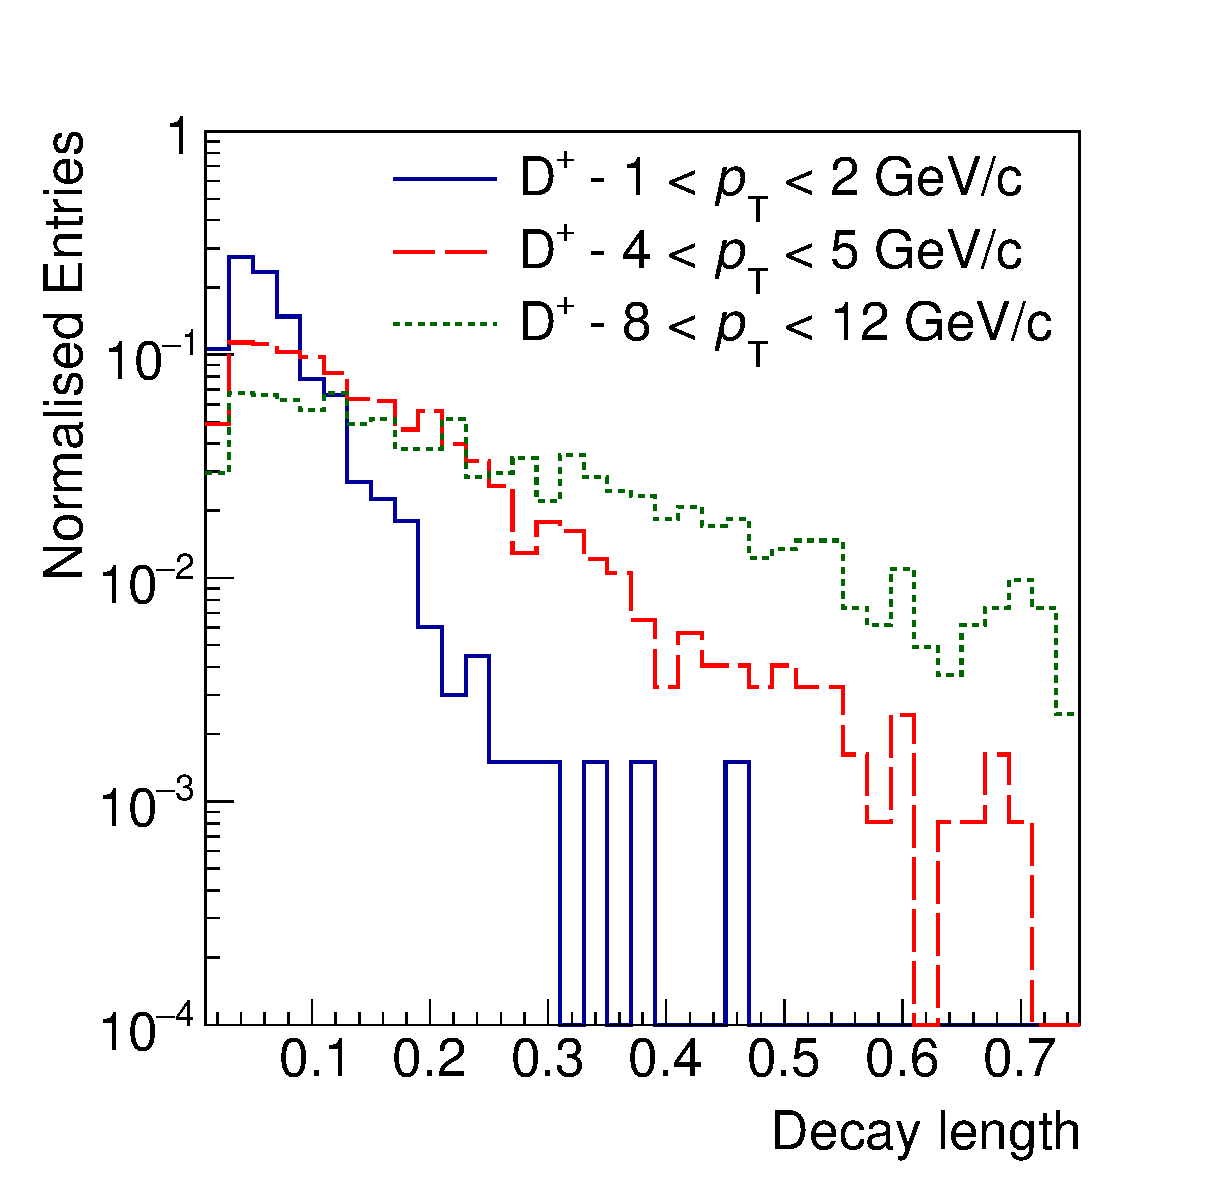
\includegraphics[scale = 0.32]{DecLCompPt.eps}}
\hspace{-0.5cm}
{\includegraphics[scale = 0.32]{NormDecLComp_4-5.eps}}
\caption{Left: reconstructed decay length distributions for D$^+$ in three different $\pt$ intervals from Monte Carlo simulations. Right: comparison between the distributions of the normalised decay length in the transverse plane for signal (prompt and feed-down D$^+$) and background.}
\label{decl}
\end{center}
\end{figure}
One of the most effective topological variables which can discriminate between the D$^+$ signal and the background is the distance between the primary and the secondary vertices, indicated as decay length, since on average it is larger for real D$^+$ than for the background candidates. Note that the distance between the reconstructed secondary and primary vertices is an approximation of the real decay length because of the curvature of the D$^+$ trajectory in the magnetic field, however it leads only to a negligible effect considering that the mean proper decay length of the D$^+$ is of the order of few hundred microns. The decay length distribution of real D$^+$ depends on the D$^+$ momentum because of the Lorentz boost, as illustrated in the left plot of figure \ref{decl}, where the decay length distributions of D$^+$ in three different transverse momentum interval are compared from Monte Carlo simulations. The decay length is also evaluated in the transverse plane, since the detector resolution is better in the $x$ and $y$ coordinates with respect to the $z$ coordinate, as discussed in section \ref{ITS_sec}. In particular, the decay length in the $xy$-plane divided by its error (\textit{normalised decay length $xy$}) is used in the selection of the D$^+$ candidates because it can provide a significant separation between signal and background, as shown in the right panel of figure \ref{decl}. 
\begin{figure}[b]
\begin{center}
{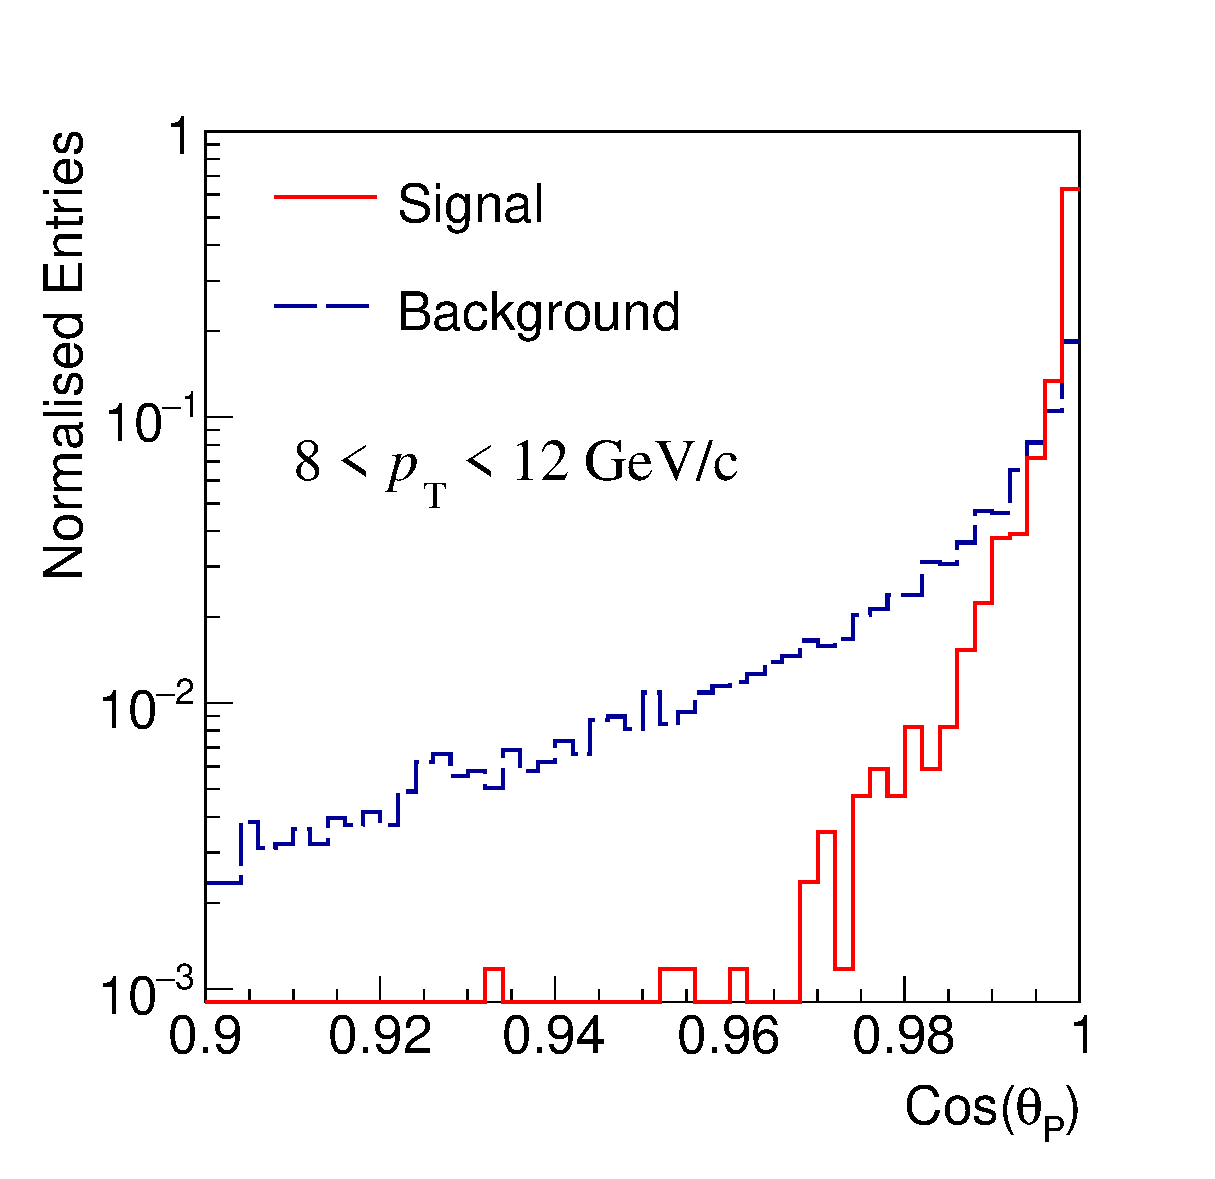
\includegraphics[scale = 0.32]{CospComp_8-12.eps}}
\hspace{-0.5cm}
{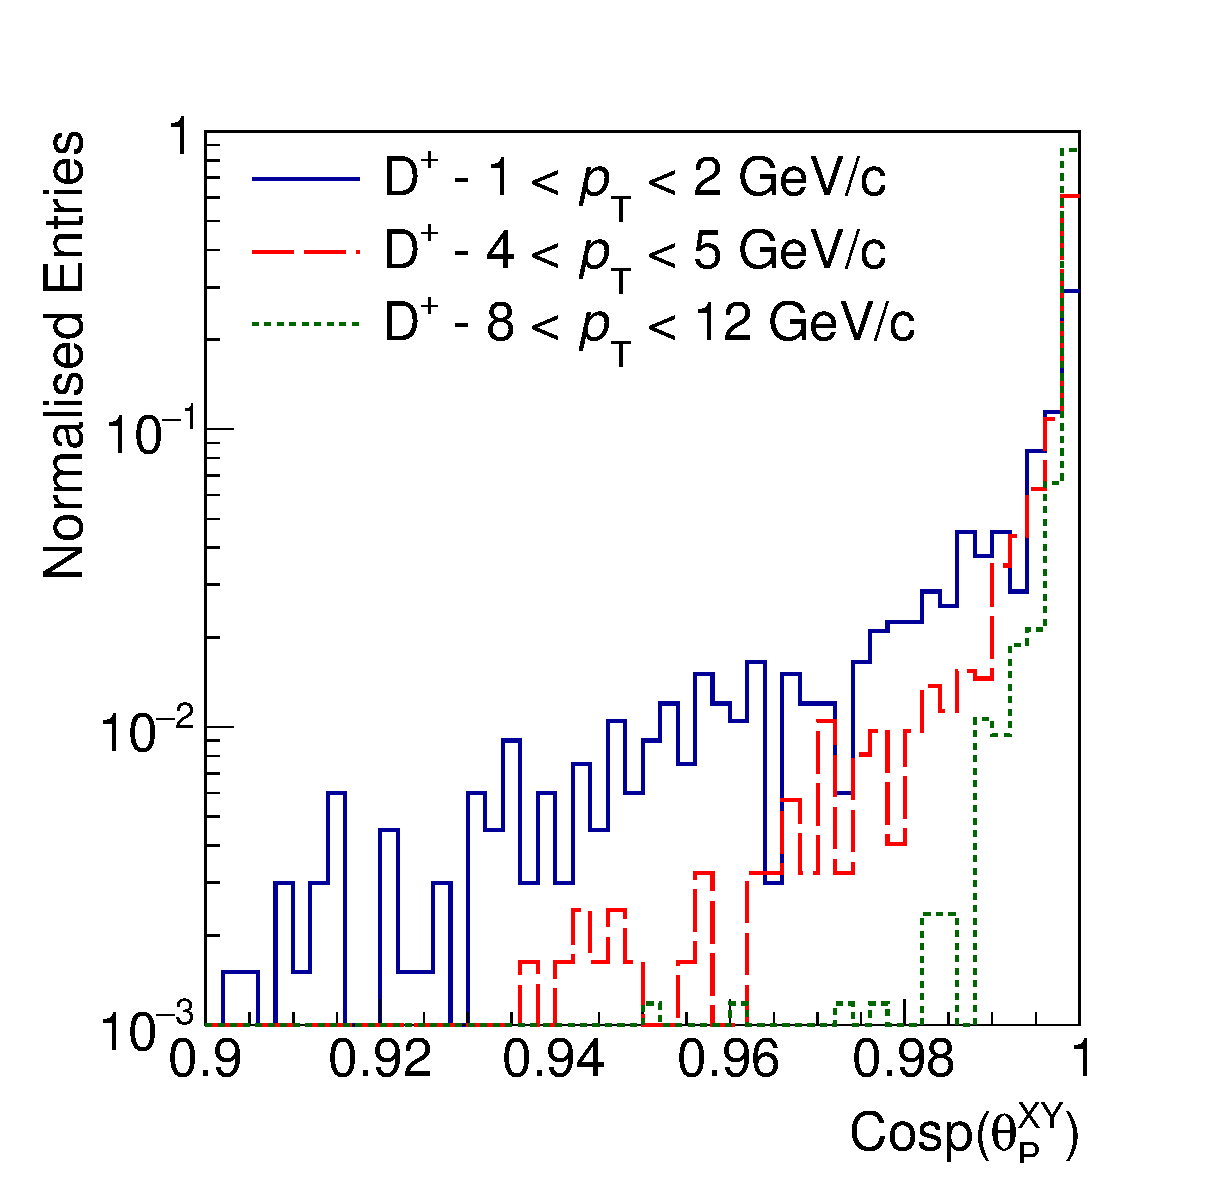
\includegraphics[scale = 0.32]{CospXYCompPt.eps}}
\caption{Left: comparison of the distribution of the reconstructed cosine of the pointing angle between signal (prompt and feed-down D$^+$) and background. Right: distributions of the reconstructed cosine of the pointing angle in the transverse plane for the D$^+$ in three different $\pt$ intervals.}
\label{cosp}
\end{center}
\end{figure}
In this plot the signal distribution, which includes the prompt and the feed-down contributions, is obtained from the MC simulation, while the background distribution from the data, using candidates in the invariant-mass region in the side-bands of the D$^+$ peak.
\subsubsection{Cosine of the pointing angle} 
The \textit{pointing angle} ($\theta_P$) is defined as the angle between the direction of the reconstructed momentum of the D$^+$ candidate and the line connecting the primary and secondary vertices, as illustrated in the sketch of the D$^+$ decay topology of figure \ref{Dplus_sketch}. Neglecting the experimental resolution on the vertices and the momentum, this variable is exactly 0 for real prompt D$^+$ and close to 0 for real feed-down D$^+$. Therefore, the distribution of the reconstructed cosine of the pointing angle is peaked at one for the signal and it is wider for the background. In the left plot of figure \ref{cosp}, the signal and background distributions of the reconstructed cosine of the pointing angle are shown for candidates with $8<\pt<12$ GeV/c. As the decay length, the $cos(\theta_P$) is evaluated also in the transverse plane, because of the better resolution achieved. In the right panel of figure \ref{cosp} it is possible to see how the distribution of $cos(\theta_P^{xy})$ of signal candidates becomes narrower with increasing D$^+$ transverse momentum. 
\subsubsection{Daughter-track dispersion around the secondary vertex}
\begin{figure}[b]
\begin{center}
{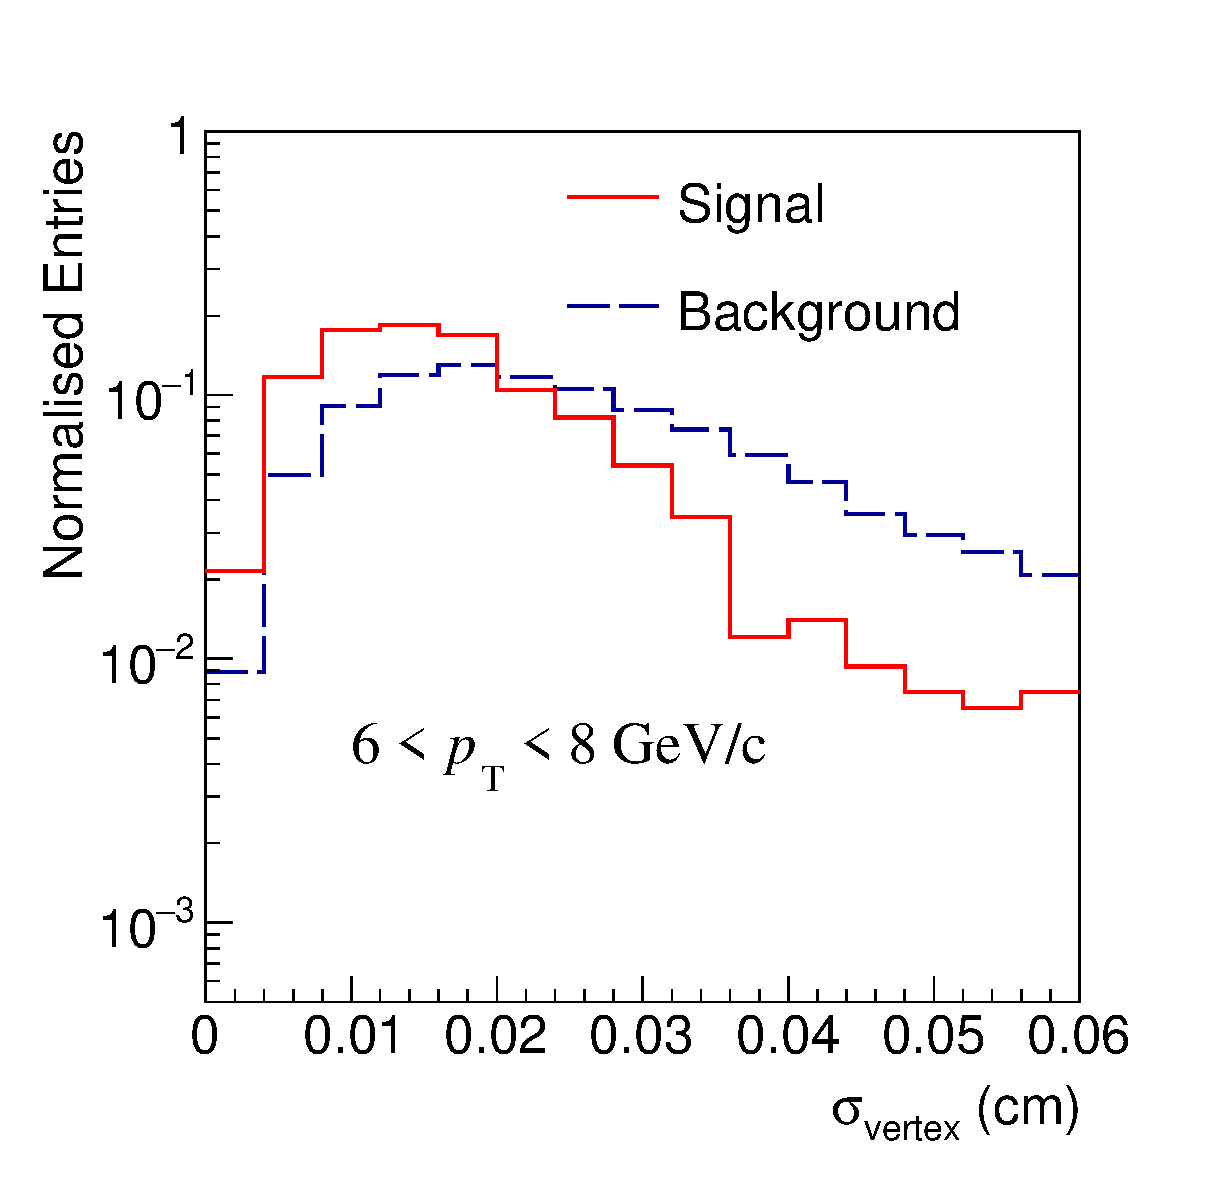
\includegraphics[scale = 0.32]{SigVtxComp_6-8.eps}}
\hspace{-0.5cm}
{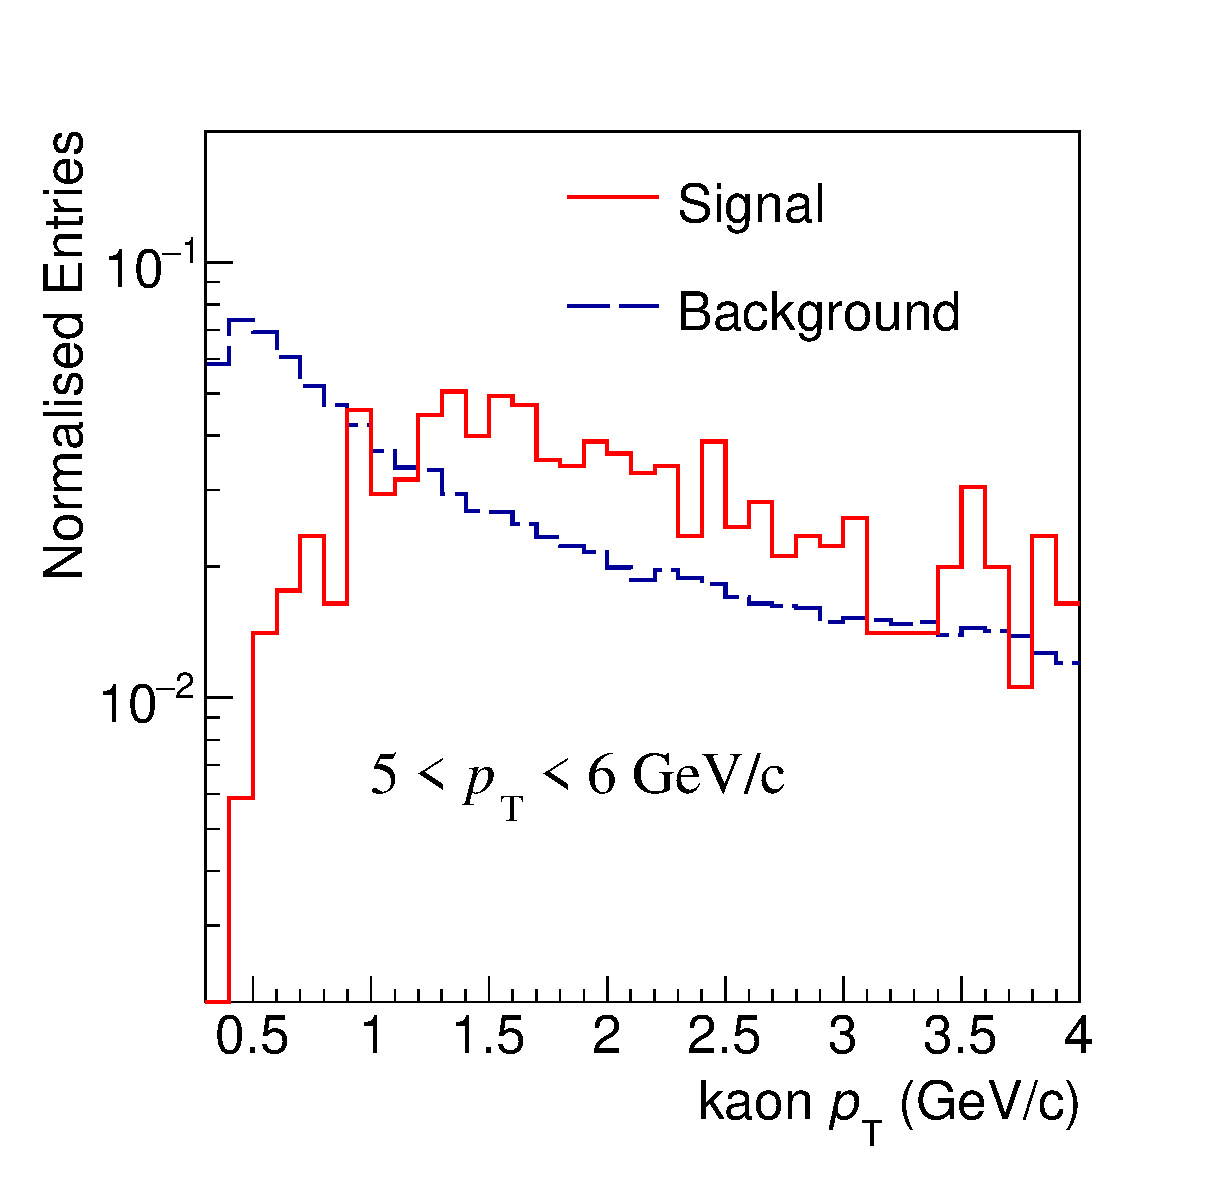
\includegraphics[scale = 0.32]{KaonPtComp_5-6.eps}}
\caption{Comparison between the distributions of reconstructed $\sigma_{vertex}$ (left) and transverse momentum of the kaon (right) of signal (prompt and feed-down D$^+$) and background candidates.}
\label{sigvtx}
\end{center}
\end{figure}
Another quantity which can be helpful in the rejection of the background is the so called \textit{sigma vertex}, defined as 
\begin{equation}
 \sigma_{vertex} = \sqrt{d_K^2+d_{\pi 1}^2+d_{\pi 2}^2},
\end{equation}
where $d_i$ are the distances of closest approach between the daughter tracks and the reconstructed secondary vertex. For real D$^+$-mesons this variable should be exactly 0, however it assumes non-zero values because of the tracking and vertexing resolution. On the contrary, for combinatorial background the three considered tracks do not come from a real D$^+$ decay vertex, and hence we expect in average a larger displacement and therefore a larger value of the $\sigma_{vertex}$, as confirmed by the distributions for signal and background shown in the left panel of figure \ref{sigvtx}. 
\subsubsection{Daughter transverse momentum}
The transverse momentum of D$^+$ decay tracks is on average larger than that of background. Therefore, a lower cut on this quantity can help to exclude a significant amount of background, keeping the majority of the signal. An example is shown in the right plot of figure \ref{sigvtx}, where the $\pt$ distributions of the kaons for signal and background candidates with $5<\pt<6$ GeV/c are compared.
\begin{table}[b]
\centering 
%\par\medskip
\begin{center} % 
\renewcommand\arraystretch{1.5} 
\fontsize{6}{8.5}\selectfont
\begin{tabular}{|c|c|c|c|c|c|c|c|c|c|}
\hline
$\pt$ (GeV/c) & [1,2] & [2,8] & [8,9] & [9,10] & [10,11] & [11,12] & [12,14] & [14,16] & [16,24]\\
\hline
$\pt^K$ (GeV/c) >& 0.3 & 0.3 & 0.3 & 0.3 & 0.3 & 0.3 & 0.3 & 0.3 & 0.3\\
$\pt^\pi$ (GeV/c) >& 0.3 & 0.35 & 0.35 & 0.35 & 0.35 & 0.35 & 0.35 & 0.35 & 0.35\\
Decay length (cm) >& 0.02 & 0.04 & 0.04 & 0.04 & 0.04 & 0.04 & 0.10 & 0.10 & 0.15\\
Norm. $L_{xy}$ >& 9 & 8 & 8 & 8 & 8 & 6 & 6 & 9 & 5\\
$cos(\theta_P)$ >& 0.990 & 0.990 & 0.990 & 0.990 & 0.990 & 0.990 & 0.990 & 0.990 & 0.990\\
$cos(\theta_P^{xy})$ >& 0.995 & 0.990 & 0.990 & 0.990 & 0.990 & 0.990 & 0.990 & 0.990 & 0.990\\
$\sigma_{vertex}$ (cm) <& 0.030 & 0.030 & 0.035 & 0.035 & 0.035 & 0.070 & 0.070 & 0.090 & 0.030\\
\hline
\end{tabular}
\caption{Summary table of the D$^+$ topological cuts optimised for the published result \cite{Abelev:2014hha}. The optimisation procedure is explained in \cite{Russo:2015xtz}.}
\label{paper_cuts}
\end{center} 
\end{table}
\subsubsection{Topological cut values used in the published result}
In table \ref{paper_cuts} I report all the values for the cuts on the described geometrical and kinematical quantities which have been applied for the standard analysis, published by the ALICE Collaboration. The choice of these cut values has been performed taking into account the stability of the raw yield extraction, the value of the efficiency obtained and the fraction of prompt D$^+$ selected.
Further details about the optimisation procedure for the cut values can be found in \cite{Russo:2015xtz}.
\subsection{Particle Identification}
The rejection of the background can be further improved by applying particle identification (PID) selection on the daughter tracks. As already mentioned in section \ref{PID_sec} the specific energy loss in the TPC and the time of flight measured with the TOF detector have been used for this purpose. For each track of the triplet, the degree of agreement with a particle hypothesis (pion, kaon or proton) is evaluated considering the number of sigmas by which the measure value deviates from the expected one. Depending on the value of $n\sigma$ in TOF and TPC, the track can be considered \textit{identified}, \textit{compatible} or \textit{rejected} as a particular particle species. The values used to obtain the response for the published result and for the analyses presented in the next Chapters are summarised in table \ref{PIDresponse}.
The D$^+$ candidates are then selected according to the following requirements:
\begin{itemize}
 \item None of the tracks has to be positively identified as a proton and simultaneously rejected as kaon or pion by either TOF or TPC.
 \item No more than one track has to be identified as a kaon and rejected as pion by either TOF and TPC.
 \item At most two tracks can be rejected as kaon by either TOF and TPC.
 \item The tracks with the same charge sign with respect to the D$^+$ candidate have to be at least compatible with the pion hypothesis for both TPC and TOF.
 \end{itemize}
\begin{table}[hb]
\centering 
\begin{center} % 
\renewcommand\arraystretch{1.2} 
\fontsize{9.}{11}\selectfont
\begin{tabular}{|c|c|c|c|}
\hline
TPC & $\pt^{trk} < 0.6$ GeV/c & $0.6 < \pt^{trk} < 0.8$ GeV/c &  $\pt^{trk} > 0.8$ GeV/c\\
\hline
$n\sigma_{TPC} < 1$ & identified & identified &compatible \\
$1 < n\sigma_{TPC} < 2$ & identified & compatible &  compatible \\
$2 < n\sigma_{TPC} < 3$ & compatible & compatible &  compatible\\
$n\sigma_{TPC} > 3$ & rejected & rejected & rejected \\
\hline
\end{tabular}
\end{center} 
\end{table}
\vspace{-0.6cm}
\begin{table}[h]
\centering 
\begin{center} % 
\renewcommand\arraystretch{1.2} 
\fontsize{9.}{11}\selectfont
\begin{tabular}{|c|c|c|}
\hline
TOF & $\pt^{trk} < 1.5$ GeV/c & $\pt^{trk} > 1.5$ GeV/c\\
\hline
$n\sigma_{TOF} < 3$ & identified & compatible \\
$n\sigma_{TOF} > 3$ & rejected & rejected \\
\hline
\end{tabular}
\caption{PID response for the TPC and TOF detectors in different $\pt$ intervals of the tracks.}
\label{PIDresponse}
\end{center} 
\end{table} 
\begin{itemize}
 \item The track with opposite charge sign with respect to the D$^+$ candidate has to be at least compatible with the kaon hypothesis for both TPC and TOF.
\end{itemize} 
If the reconstructed transverse momentum of the candidate is smaller than 2 GeV/c, the last two selections require the tracks to be positively identified instead of just being compatible with the particle hypothesis. This stronger requirement is needed because of the large amount of background, which is widely dominant in this $\pt$ region.  
\subsection{Raw yield extraction}
\begin{figure}[b]
\begin{center}
{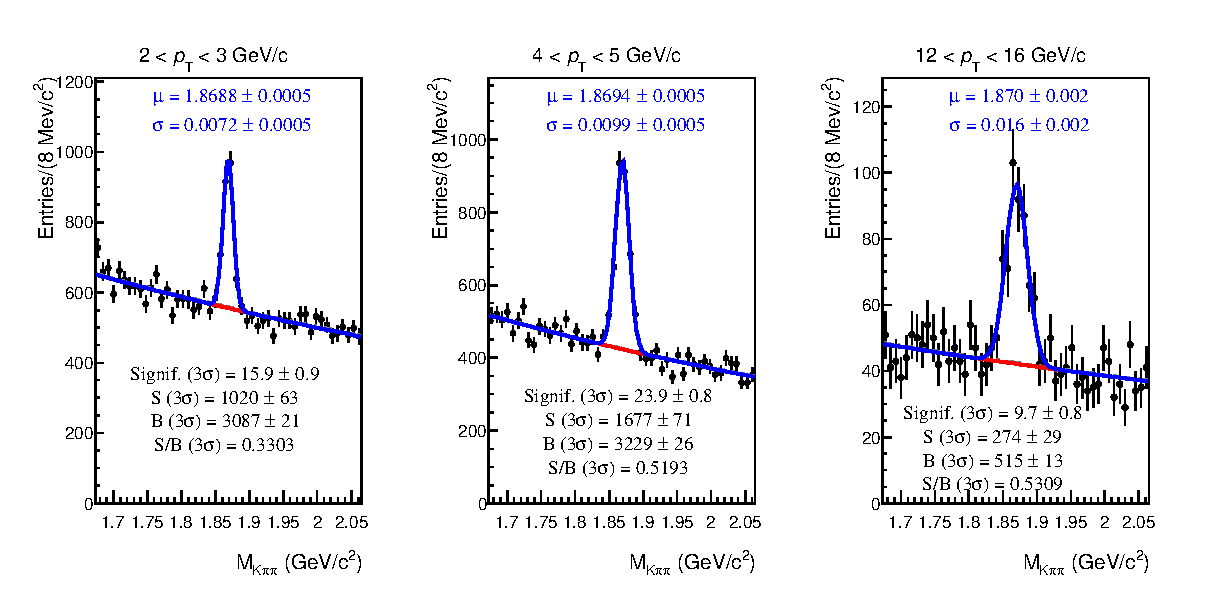
\includegraphics[scale = 0.65]{MassFit3Bin.eps}}
\caption{Invariant-mass fits in the transverse momentum intervals $2 < \pt < 3$ GeV/c, $4 < \pt < 5$ GeV/c and $12 < \pt < 16$ GeV/c obtained applying the topological cuts reported in table \ref{paper_cuts} and the PID selection.}
\label{massfitex}
\end{center}
\end{figure}
In figure \ref{massfitex} are shown three example of fit performed to the invariant-mass distributions of the D$^+$-meson candidates (and their charge conjugates) in three different D$^+$ transverse momentum intervals, obtained applying the topological cuts in table \ref{paper_cuts} and the particle identification. The signal is parametrised with a Gaussian, while the background with an exponential function. The stability of the fit parameters was checked by comparing the Gaussian mean and width with the values obtained by fitting the MC distributions. As it can be seen in figure \ref{massfitex} the Gaussian width increases with increasing $\pt$, as expected from the transverse-momentum resolution. Thanks to the topological cuts, the signal-to-background ratio and the significance, defined as
\begin{equation}
significance = \frac{S}{\sqrt{S+B}},
\end{equation}
are maximised. The best significance is achieved at intermediate values of transverse momentum, while it is lower at low $\pt$ because of the large combinatorial background and at high $\pt$ because of the poorer statistics.  
\section{Prompt and Feed-down D$^+$}
As discussed in section \ref{HF_AA} the interaction with the medium is different for charm and beauty quarks, because of their different masses. Therefore in the D$^+$-meson measurement one should separate the \textit{prompt} contribution (D$^+$ originated directly from the hadronisation of a $c$-quark, or from the decay of an excited open charm or charmonimum state) from the \textit{feed-down} contribution (D$^+$ coming from the decay of a B-hadron). This can be done with two different approaches: the first one, which was used for the standard analysis \cite{Abelev:2014hha}, is a \textit{theory-driven} method, which consists on the evaluation of the fraction of D$^+$ prompt making use of pQCD calculations and of the prompt and feed-down D$^+$ efficiencies from Monte Carlo Simulations. On the other hand it is also possible to apply \textit{data-driven} methods that exploit the different shapes of the distributions of quantities related to the decay topology, which can discriminate between prompt and feed-down D$^+$. In particular the development of data-driven methods for the measurement of the D$^+$ prompt fraction is the main topic of thesis and will be presented in Chapter \ref{IP_chapter} and \ref{CV_chapter}.   
\subsection{Theory-driven methods for the D$^+$ prompt fraction evaluation}
\label{Theory-driven}
\begin{figure}[t]
\begin{center}
{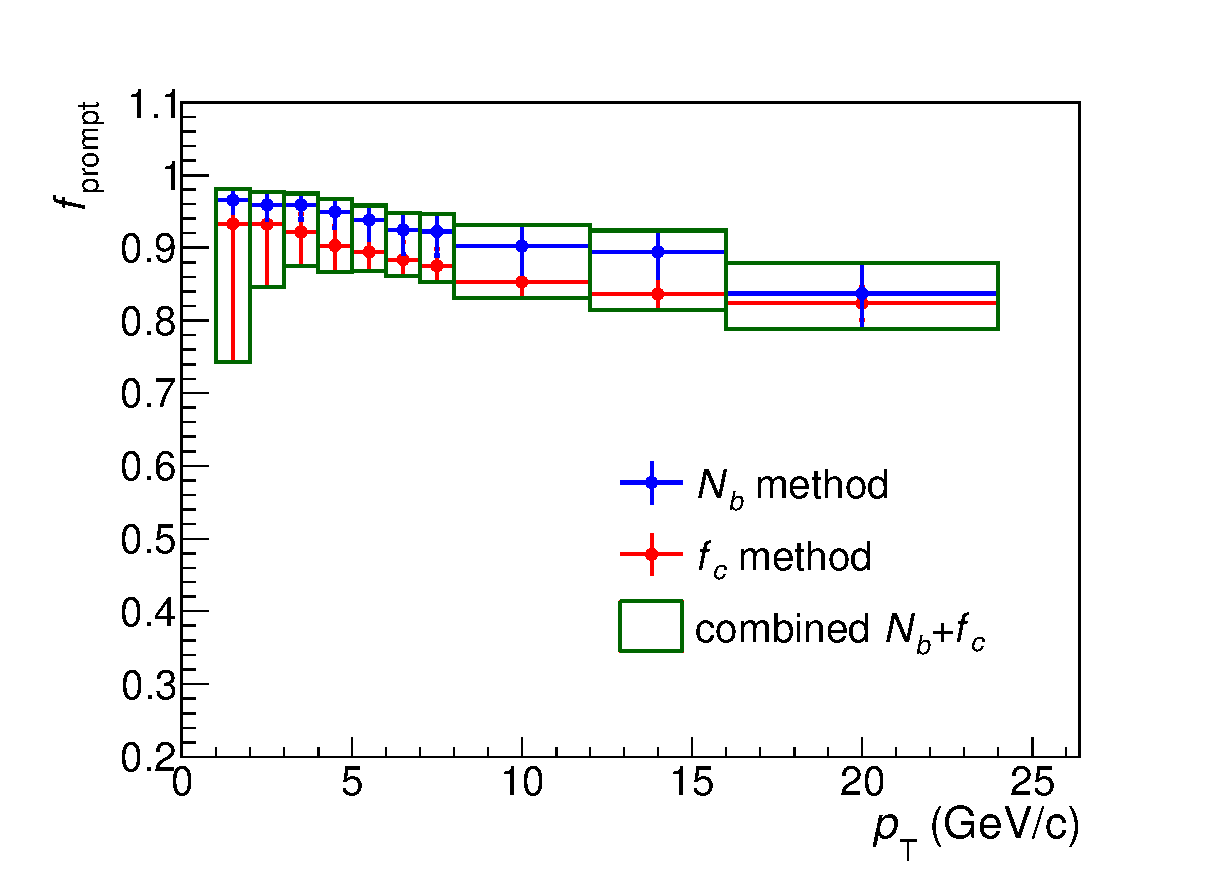
\includegraphics[scale = 0.4]{Fprompt_fc_Nb_comp.eps}}
\caption{D$^+$ prompt fraction $f_{prompt}$ evaluated with the theory-driven methods $f_c$ and $N_b$ for the set of topological cuts reported in table \ref{paper_cuts}.}
\label{fprompt_FONLL}
\end{center}
\end{figure}
The prompt fraction of D$^+$-mesons $f_{prompt}$ can be calculated using two different theory-driven methods, both based on FONLL pQCD calculations. The usage of FONLL calculations is supported by the observation (see section \ref{HF_prod_sec}) that they describe the $\pt$-differential cross section measured in pp collisions. According to the first approach (called $N_b$ method), the prompt fraction is defined as
\begin{equation}
\begin{split}
 f_{prompt} = 1-A \cdot\bigg{(}\frac{d^2\sigma}{d\pt dy}\bigg{)}^{FONLL}_{feed-down}\cdot R_{pPb}^{feed-down}(\pt) \times\\[0.5cm] \times\frac{(Acc\times\epsilon)_{feed-down} \cdot \Delta y \cdot \Delta \pt \cdot BR \cdot L_{int}}{N^{D^\pm}_{raw}/2},
\end{split}
\end{equation}
where $A$ is the mass number of the Pb nucleus, $(Acc\times\epsilon)_{feed-down}$ is the product of acceptance and efficiency for feed-down D$^+$ evaluated with the MC simulation described in the next section, $\Delta \pt$ and $\Delta y$ are the widths of the transverse momentum and rapidity intervals, $BR$ is the branching ratio of the considered decay channel, $L_{int}$ the integrated luminosity and $N_{raw}^{D^\pm}$ is the raw yield extracted from the invariant-mass fits described above. The feed-down D$^+$ cross section $\bigg{(}d^2\sigma/d\pt dy\bigg{)}$ is evaluated from the B-meson cross section in pp collisions at $\sqrt{s}=$ 5.02 TeV estimated with FONLL and subsequently using the EvtGen package \cite{Lange:2001uf} to describe the B $\rightarrow$ D + X kinematics. The nuclear modification factor $R_{pPb}^{feed-down}(\pt)$ is assumed equal to the one for prompt D$^+$, on the basis of calculations including initial state effects, since it was never measured. \\\\
The alternative method for the computation of $f_{prompt}$, called $f_c$, needs as input also the FONLL differential cross section, the nuclear modification factor and the acceptance times efficiency for prompt D$^+$-mesons:
\begin{equation}
 f_{prompt} = \bigg{(}1+\frac{\frac{d^2\sigma}{d\pt dy}^{FONLL}_{feed-down}\cdot (Acc\times\epsilon)_{feed-down}\cdot R_{pPb}^{feed-down}(\pt)}{\frac{d^2\sigma}{d\pt dy}^{FONLL}_{prompt}\cdot (Acc\times\epsilon)_{prompt}\cdot R_{pPb}^{prompt}(\pt)}\bigg{)}^{-1}.
\end{equation}
It is important to notice that the prompt fraction depends on the D$^+$ transverse momentum because of the different shape of the FONLL $\pt$-differential cross section of prompt and feed-down D$^+$ and the topological selections which lead to a $\pt$-dependent efficiency. 
For the central value of $f_{prompt}$, the $N_b$ method is used, in light of the fact that the measured B-meson cross-section is in good agreement with FONLL, lying close to the central value of the theoretical calculation, while the D-meson one is found to lie on the upper edge of the FONLL uncertainty band (see section \ref{HF_prod_sec}). The $f_c$ method is kept in order to evaluate a systematic uncertainty, as shown in figure \ref{fprompt_FONLL}. The other main sources of systematics of $f_{prompt}$ come from the perturbative calculation of the cross sections and the assumption on nuclear modification factor for feed-down D$^+$, which is varied in the range $ 0.9 < R_{pPb}^{feed-down}/R_{pPb}^{prompt} < 1.3$ in order to evaluate an uncertainty. 
\section{The Monte Carlo simulation}
\label{MC_sec}
The Monte Carlo simulation is needed to evaluate the efficiency and acceptance factors used to correct the measured raw yields and it is also used to obtain the distribution templates for the analysis presented in Chapter \ref{IP_chapter}. \\
The MC sample used is based on pp events generated with Pythia v6.4.21 with the Perugia-0 \cite{Skands:2009zm} tune with at least a $c\bar{c}$ or a $b\bar{b}$ pair in each event. In order to make the multiplicity distribution in the MC more realistic, a number of binary collisions is extracted from a Glauber MC simulation of p-Pb collisions and, if larger than 1, a HIJING \cite{Wang:1991hta} p-Pb event is added as underlying event to the Pythia one. After the particle generation, the GEANT3 transport package is used to simulate the interaction with the detector. The detector response is modelled using AliRoot \cite{AliRootBib}, the software adopted by the ALICE offline project. AliRoot is an object-oriented code based on Root \cite{RootBib}, a software specifically designed for the data analysis of high energy physics experiments. AliRoot provides the packages to perform event generation, detector simulation event reconstruction and data analysis. In particular, for the generation of the MC sample used in this analysis, the description of the detector was designed in order to match the experimental conditions for all the sub-systems during the 2013 p-Pb data taking period. 
\subsection{Efficiency and Acceptance}
\label{effacc_sec}
\begin{figure}[tb]
\begin{center}
{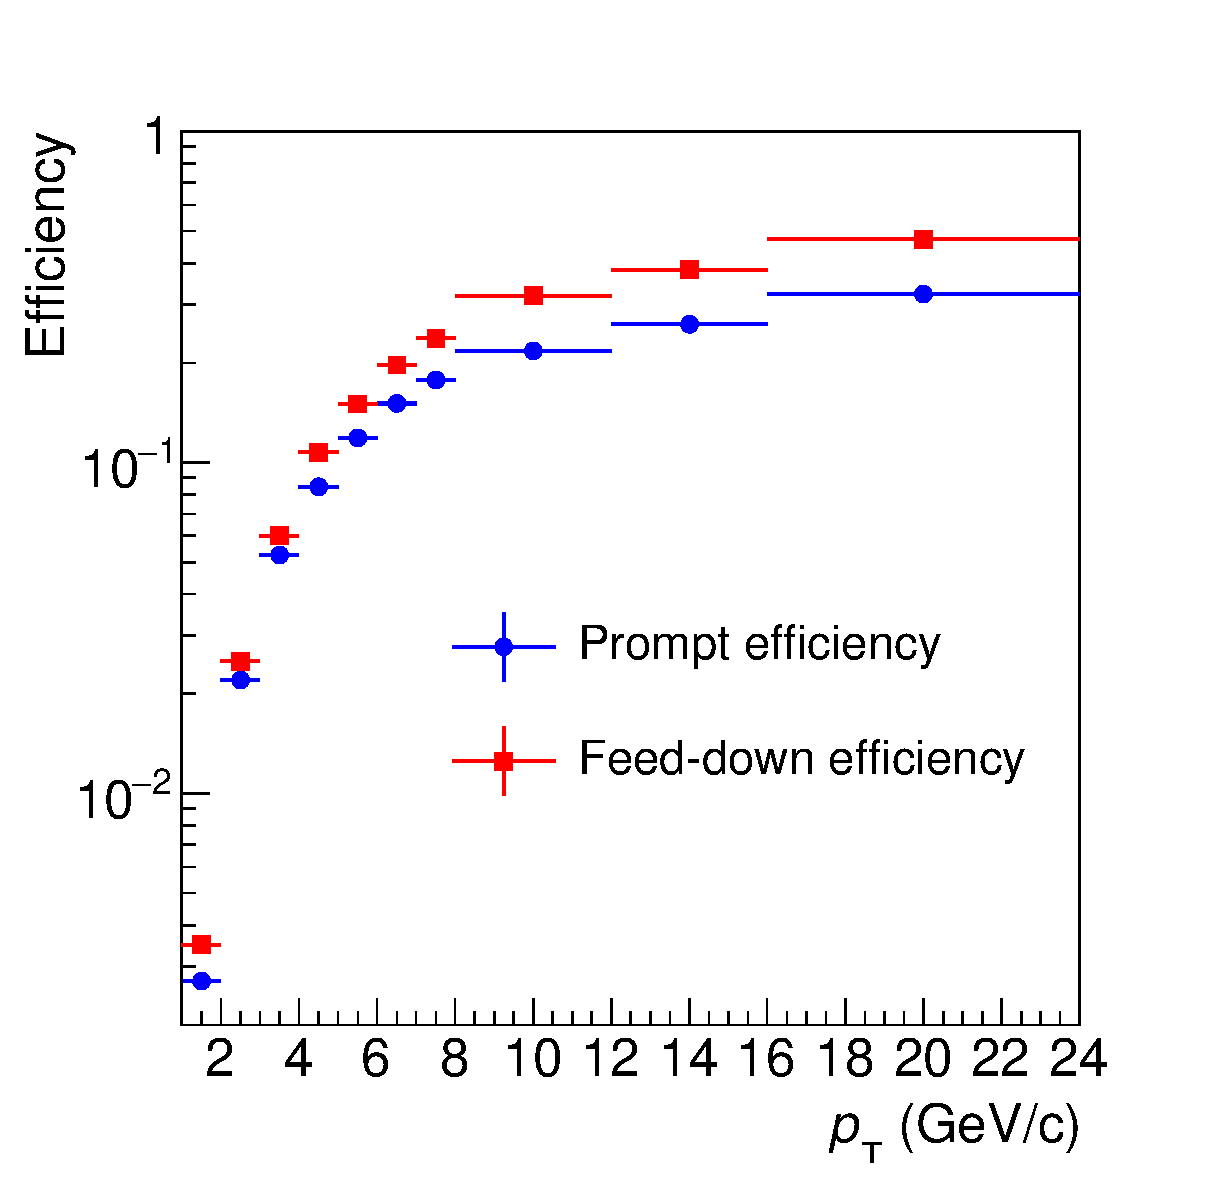
\includegraphics[scale = 0.32]{Eff_Dplus_PaperCuts.eps}}
\hspace{-0.5cm}
{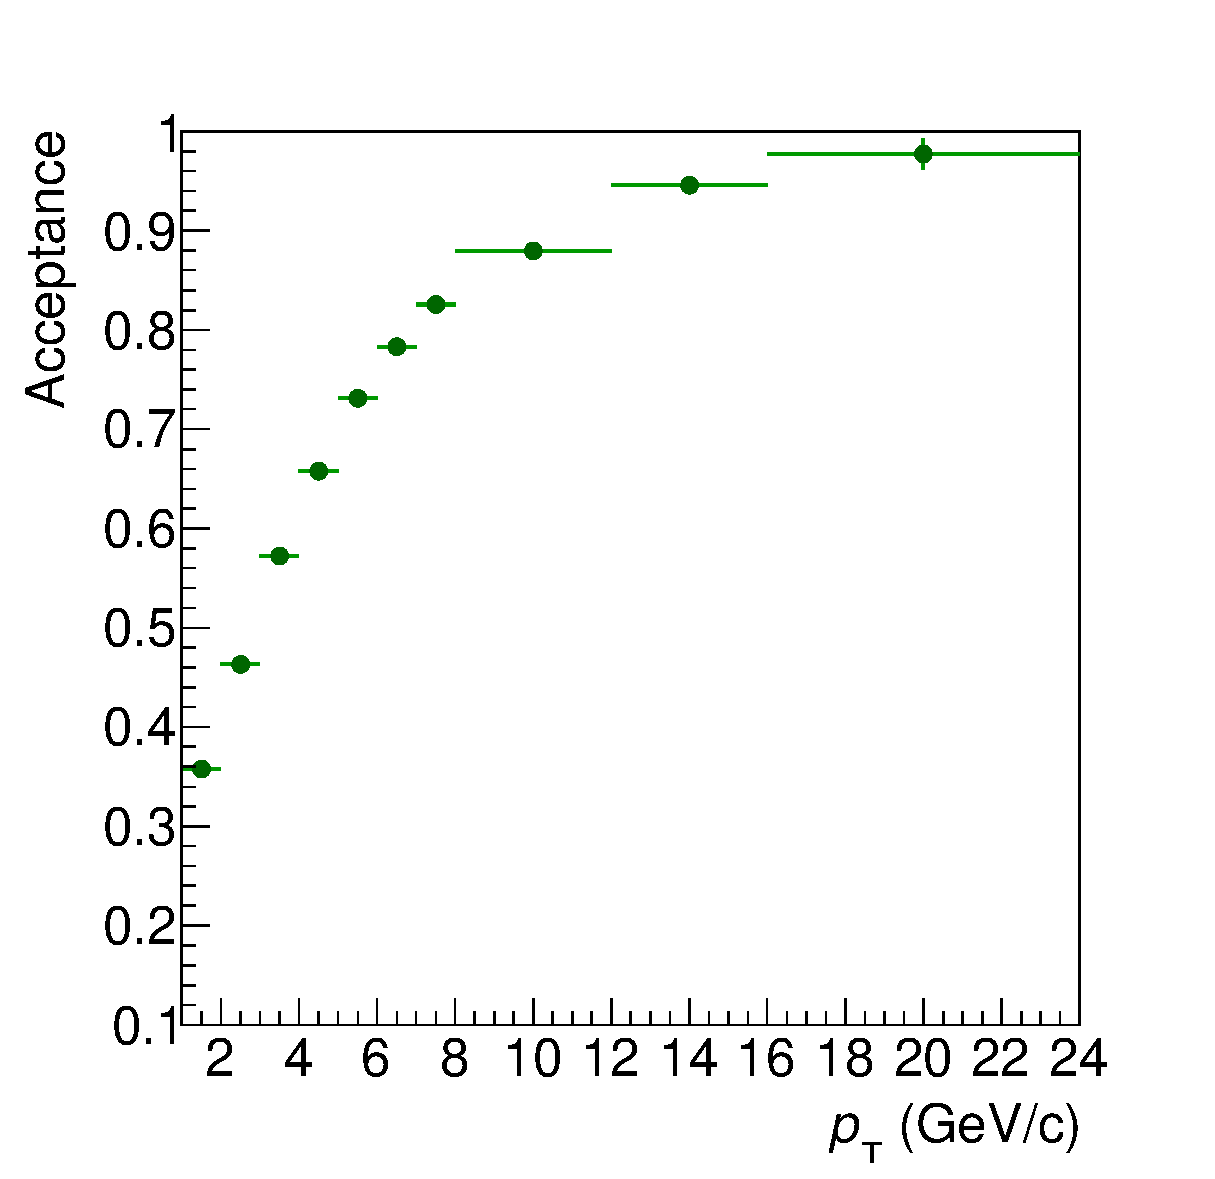
\includegraphics[scale = 0.32]{Acc_Dplus.eps}}
\caption{Left: the reconstruction efficiency as a function of $\pt$ for prompt and feed-down D$^+$ obtained applying the topological cuts in table \ref{paper_cuts} and the PID. Right: the acceptance factor for prompt D$^+$-mesons as a function of $\pt$.}
\label{effacc_paper}
\end{center}
\end{figure}
The efficiency and acceptance factors for the raw yield correction are evaluated with the MC sample described above. In particular the efficiency is defined as the number of reconstructed D$^+$, after all the topological and PID selections, divided by the number of generated D$^+\rightarrow$ K$^-\pi^+\pi^+$ decays with the three daughters which fulfil the acceptance requirements of $|\eta| <0.9$ and $\pt > 0.1$ GeV/c for events with the $z$-coordinate of the generated primary vertex within 10 cm from the nominal interaction point. Furthermore, the acceptance is evaluated as the ratio between the number of the generated D$^+\rightarrow$ K$^-\pi^+\pi^+$ with the three daughters in the acceptance and the D$^+\rightarrow$ K$^-\pi^+\pi^+$ generated in the rapidity range $|y| < y_{fid}$, for events with $|Z_{GenVertex}| < 10$ cm. In figure \ref{effacc_paper} the efficiencies for prompt and feed-down D$^+$ obtained applying the topological cuts reported in table \ref{paper_cuts} and the PID selection (left) and the acceptance (right) are shown as a function of the transverse momentum. The efficiency for D$^+$ coming from B-hadron decays is higher that that of prompt D$^+$ because of the position of their decay vertex, which is on average more displaced from the primary vertex with respect to the one for prompt D$^+$. 
\section{Results from the standard analysis}
In this section I present the result obtained with the theory-driven method for the evaluation of the D$^+$ prompt fraction, which is published by the ALICE Collaboration \cite{Abelev:2014hha}. The prompt D$^+$ $\pt$-differential cross section was measured applying all the event, track, topological and PID selections described in this Chapter, starting from the raw yield $N_{raw}^{D^\pm}|_{y<y_{fid}}$ and correcting for the acceptance and efficiencies factors (see \cite{Russo:2015xtz} for more details). In particular the cross section is computed as:
\begin{equation}
\frac{d\sigma^{D^+}_{prompt}}{dpt}\bigg{|}_{y<0.5} = \frac{1}{2}\cdot\frac{f_{prompt}\cdot N_{raw}^{D^\pm}|_{|y|<y_{fid}}}{\Delta \pt \Delta y}\cdot\frac{1}{(Acc\times\epsilon)_{prompt}(\pt)}\cdot\frac{\sigma^{pPb}_{MB}}{BR\cdot N_{ev}}.
\label{promptcross_eq}
\end{equation}
\begin{figure}[tb]
\begin{center}
{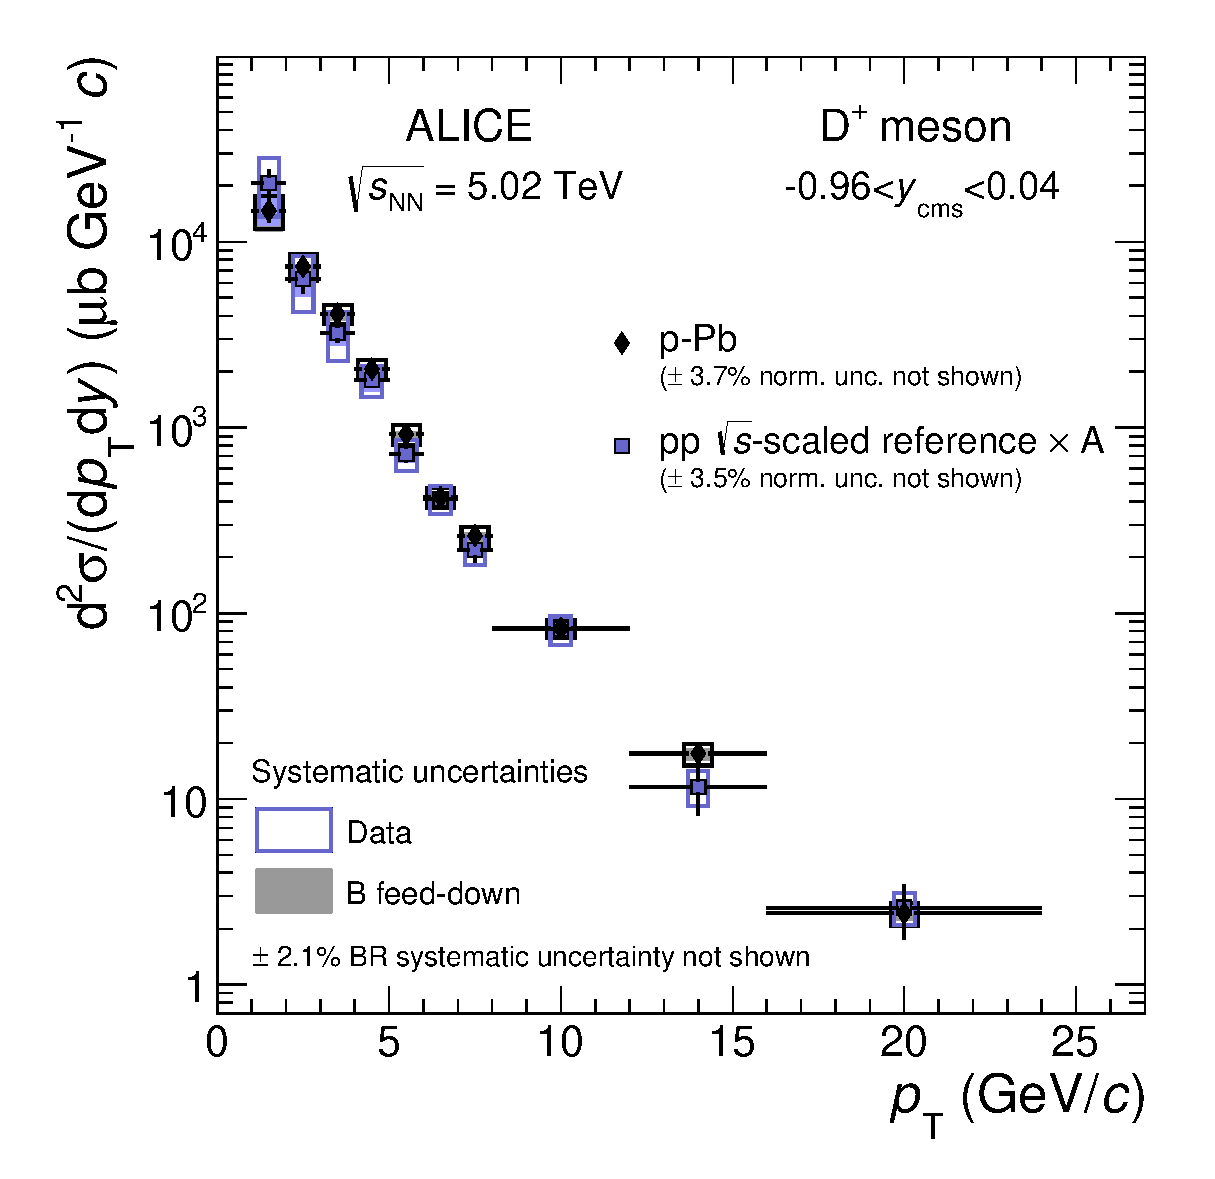
\includegraphics[scale = 0.4]{Dplus-dsigmadpt-pPb.eps}}
\caption{Prompt D$^+$ $\pt$-differential production cross section measured by the ALICE Collaboration in p-Pb collisions at $\sqrt{s_{NN}}=5.02$ TeV compared to the pp reference cross section scaled by the Pb mass number $A=208$ \cite{Abelev:2014hha}.}
\label{paper_result}
\end{center}
\end{figure} In the formula above the factor $1/2$ takes into account the fact that the raw yields include particles and anti-particles, $f_{prompt}$ is evaluated with the $N_b$ method, and $BR$ is the branching ratio of the decay channel D$^+ \rightarrow$ K$^-\pi^+\pi^+$. The width of the fiducial acceptance coverage $\Delta y = 2y_{fid}$ is common for all the transverse momentum intervals $\Delta \pt$ measured. The $\sigma^{pPb}_{MB}$ is the Minimum Bias trigger cross section from van der Meer scans and $N_{ev}$ is the number of accepted events. This number has to include the events with the primary vertex which fulfils the condition $|Z_{vertex}|<10$ cm but is not reconstructed. This is necessary because the efficiency and acceptance factors take into account all the events with $|Z_{GenVertex}|<10$ cm independently if the primary vertex is reconstructed or not in the event. Therefore the number of events for normalisation is computed as
\begin{equation}
\fontsize{9}{11}\selectfont
\begin{split}
N_{ev} = N_{RecoVert}(|Z_{RecoVert}|<10\text{ cm}) + N_{NoVert}(|Z_{RecoVert}|<10\text{ cm}) =\\
= N_{RecoVert}(|Z_{RecoVert}|<10\text{ cm})+N_{RecoVert}^{Tot} - N_{NoVert}(|Z_{RecoVert}|>10\text{ cm})=\\
= N_{RecoVert}(|Z_{RecoVert}|<10\text{ cm})+N_{RecoVert}^{Tot} - N^{Tot}_{NoVert}\frac{N_{NoVert}(|Z_{RecoVert}|>10\text{ cm}}{N^{Tot}_{RecoVert}}.
\label{norm_factor_eq}
\end{split}
\end{equation}
The final result is shown in figure \ref{paper_result}, compared to the pp reference cross section scaled by the Pb mass number $A=208$. Since a measurement of the $\pt$-differential cross section at the same centre-of-mass energy was not available, the one measured at $\sqrt{s} = 7$ TeV was used, scaling it to $\sqrt{s} = 5.02$ TeV according to the FONLL calculations. One of the main source of uncertainty for this measurement, especially at low $\pt$, comes from the evaluation of the prompt fraction with the FONLL-based methods described in section \ref{Theory-driven} (shaded box in the plot). This is the motivation for the studies presented in the next Chapters, since the development of data-driven feed-down subtraction approaches aims to reduce these uncertainties and to avoid the usage of theoretical calculations in the D$^+$ prompt fraction evaluation.
\chapter{Impact-parameter fit method for the prompt D$^+$ fraction determination}
\label{IP_chapter}
In this Chapter I will present the main data-driven method that I developed for the evaluation of D$^+$ prompt fraction. The main advantage of this technique is that it does not rely on any theoretical assumption, unlike the FONLL-based methods presented in section \ref{fprompt_FONLL}. It also aims to reduce the large systematic uncertainty of the theory-driven approach, especially at low transverse momentum.
\begin{figure}[htb]
\begin{center}
{\includegraphics[scale = 0.25]{FD_sketch.png}}
\hspace{0cm}
{\includegraphics[scale = 0.25]{Prompt_sketch.png}}
\caption{Sketch of the decay topology for prompt (right) and feed-down (left) D$^+$ with particular emphasis on the true impact parameter.}
\label{IP_topology}
\end{center}
\end{figure}
This first data-driven method exploits the different shapes of the impact-parameter distributions for prompt and feed-down D$^+$. The impact parameter is defined as the distance of closest approach between the prolonged momentum direction of the D$^+$-meson and the primary vertex. Since the prompt D$^+$-mesons come from the primary vertex, their real impact parameter is by definition exactly zero. Therefore, we can expect the measured distribution to be centred at zero and smeared for resolution effects. On the other hand, the impact parameter for feed-down D$^+$ is in general different from zero and it depends on the decay length of the B-hadron and its relative direction with respect to the D$^+$-meson. In figure \ref{IP_topology} is illustrated an example of decay and the corrispective true impact parameter for both prompt and feed-down D$^+$-mesons. Beside that, there is an alternative data-driven method, that will be presented in Chapter \ref{CV_chapter}. 
\section{Analysis strategy}
Before to start with the description of the analysis, I would like to introduce the strategy adopted. First and foremost, all the selections applied (event, track quality, topological cuts and PID) are the same as those used for the standard analysis (see Chapter \ref{Dplus_reco}). This is very important in order to be able to compare the two results, since the prompt fraction depends on the topological cuts applied.\\ Then, the procedure is divided in two main steps: 
\begin{itemize}
 \item A prefit phase, which consists in the parametrisation of the impact-parameter distributions in the transverse plane ($d_{0}^{xy}$) for the three different types of candidates that contribute to the measured distribution: prompt D$^+$, feed-down D$^+$ and background. For the prompt and feed-down D$^+$ the distributions are obtained from the Monte Carlo sample described in section \ref{MC_sec}. The distribution for the combinatorial background is directly taken from the data sample (see section \ref{datasample}), in the invariant-mass region aside the D$^+$ peak (see section \ref{SB_sec}).
 Each contribution is fitted with a specific function, which is called \textit{template}.
 \item An unbinned log-likelihood fit to the impact-parameter distributions in the data using the templates obtained in the previous step.
\end{itemize}
All the parameters obtained in the prefit phase are fixed in the final fit on data, except for the detector-resolution term which is kept free in order to compensate a possible not perfect description of the impact-parameter resolution in the MC simulation (a detailed description will be provide in section \ref{prompt_prefit_sec}).\\ This method requires a certain amount of statistics in order to obtain a stable fit result, therefore the transverse momentum range considered for this analysis is narrower ($2<\pt<16$ GeV/c instead of $1<\pt<24$ GeV/c) with respect to the one used for the standard analysis obtained with the theory-driven approach, presented in section \ref{paper_result}. 
\section{Prefit on the impact-parameter distributions}
\label{prefit_sec}
In this section I will present the prefits performed to the impact-parameter distributions in the transverse plane for prompt and feed-down D$^+$-mesons and for the combinatorial background. 
\subsection{MC impact-parameter distributions for prompt D$^+$}
\label{prompt_prefit_sec}
\begin{figure}[tb]
\begin{center}
{\includegraphics[scale = 0.31]{ImpParPrompt_2-3.eps}}
\hspace{-0.2cm}
{\includegraphics[scale = 0.31]{ImpParPrompt_8-12.eps}}
\caption{Examples of fit to the simulated impact-parameter distributions for prompt D$^+$-mesons in two different $\pt$ intervals.}
\label{prompt_prefit}
\end{center}
\end{figure}
The impact-parameter distributions in the transverse plane for prompt D$^+$ were obtained from the Monte Carlo simulation described in section \ref{MC_sec}, in seven $\pt$ intervals in the range $2<\pt<16$ GeV/c. Since the generated impact parameter for prompt D$^+$-mesons is by definition zero, the distributions from the reconstruction of the MC data (\textit{simulated} distributions) are approximately Gaussian due to the finite track and primary vertex resolution of the detector.  
However, as shown in figure \ref{prompt_prefit}, they clearly present non-Gaussian tails, which are more prominent at higher D$^+$ transverse momentum. For this reason, a simple Gaussian function would not give a proper description of the distribution and therefore the fit function used is the sum of a Gaussian and a symmetric exponential function
\begin{equation}
\begin{split}
F^{prompt}&(d_0^{xy}) = F^{g+exp}(d_0^{xy}) =\\
&=N\cdot \bigg\{\frac{f_{gaus}^{prompt}}{\sqrt{2\pi}\sigma_{prompt}}e^{-\frac{(d_0^{xy}-\mu_{prompt})^2}{2\sigma_{prompt}^2}}+\frac{1-f_{gaus}^{prompt}}{2\lambda_{prompt}}e^{-\frac{|d_0^{xy}-\mu_{prompt}|}{\lambda_{prompt}}}\bigg\},
\label{prompt_func}
\end{split}
\end{equation}
where $N$ is a normalisation factor which is fixed to the integral of the histogram, $f_{gaus}^{prompt}$ represents the fraction of the integral contained in the Gaussian function, $\mu_{prompt}$ is the common mean value for the two contributions, $\lambda_{prompt}$ is the slope of the exponential function and $\sigma_{prompt}$ is the width of the Gaussian function, which represents the resolution of the detector. As shown in the two examples in figure \ref{prompt_prefit}, the $\chi^2$ values show that the chosen functional form gives a reasonably good description of the distributions. Furthermore, it is possible to notice how the Gaussian width decreases with increasing D$^+$ transverse momentum, due to the better impact-parameter resolution on high $\pt$ tracks (right panel of figure \ref{tracking}). Also the $f_{gaus}^{prompt}$ parameter decreases with increasing $\pt$, because of the higher contribution in the exponential. All the other fits to the impact-parameter distributions for prompt D$^+$ in the $\pt$ intervals considered for the analysis can be found in the appendix \ref{prompt_prefit_appendix}.
\subsection{MC impact-parameter distributions for feed-down D$^+$}
\begin{figure}[tb]
\begin{center}
{\includegraphics[scale = 0.31]{ImpParTrueFD_5-6.eps}}
\hspace{-0.2cm}
{\includegraphics[scale = 0.31]{ImpParTrueFD_12-16.eps}}
\caption{Examples of fit to the true generated impact-parameter distributions for feed-down D$^+$-mesons in two different $\pt$ intervals.}
\label{trueFD_prefit}
\end{center}
\end{figure}
The true impact parameter for the feed-down D$^+$-mesons is different from zero because in general the momentum of the D$^+$ is not parallel to the one of the B-hadron, as shown in the left panel of figure \ref{IP_topology}. In particular it depends on the decay length of the B-hadron and the angle between the directions of the two particles. For this reason the impact-parameter distribution of feed-down D$^+$ is more difficult to parametrise with respect to the one of prompt D$^+$. In order to achieve a satisfactory description of the distribution, two steps were performed. First, the true impact-parameter distribution in the $xy$-plane for feed-down D$^+$ from the Monte Carlo simulation in the seven $\pt$ intervals of the analysis, applying all the selections described in Chapter \ref{Dplus_reco}, was fitted with a double exponential function, symmetrised with respect to its mean value 
\begin{equation}
F^{feed-down}_{true}(d_0^{xy}) = N \cdot \bigg\{\frac{f_{\lambda_1}^{FD}}{2\lambda_1^{FD}}e^{-\frac{|d_0^{xy}-\mu_{FD}|}{\lambda_1^{FD}}}+\frac{1-f_{\lambda_1^{FD}}}{2\lambda_2^{FD}}e^{-\frac{|d_0^{xy}-\mu_{FD}|}{\lambda_2^{FD}}}\bigg\},
\label{trueFD_func}
\end{equation}
where $N$ is again fixed to the integral of the histogram, $\lambda_1^{FD}$ and $\lambda_2^{FD}$ are the slopes of the two symmetrised exponential functions, $f_{\lambda_1}^{FD}$ is the fraction of integral contained in the first function and $\mu_{FD}$ is the common mean value. The impact-parameter range in the fit increases with the transverse momentum, starting from $[-250,250]$ $\mu$m in the interval $2<\pt<3$ GeV/c up to $[-450,450]$ $\mu$m in $12<\pt<16$ GeV/c, in order to get a good description of the distribution in the steepest region. Two examples of fit to the true impact-parameter distribution for feed-down D$^+$ are presented in figure \ref{trueFD_prefit}. The reasonable agreement between the functional form chosen and the distributions is confirmed by the $\chi^2$ values obtained. 
\begin{figure}[tb]
\begin{center}
{\includegraphics[scale = 0.31]{ImpParRecoFD_5-6.eps}}
\hspace{-0.3cm}
{\includegraphics[scale = 0.31]{ImpParRecoFD_12-16.eps}}
\caption{Examples of reconstructed impact-parameter distributions for feed-down D$^+$-mesons in two different $\pt$ intervals. The function superimposed is the convolution between the true impact parameter function for feed-down D$^+$ (eq. \ref{trueFD_func}) and the resolution term (eq. \ref{prompt_func}).}
\label{recoFD_prefit}
\end{center}
\end{figure}
The second step for the parametrisation consisted in a convolution of the function obtained for the feed-down D$^+$ true impact-parameter distribution $F_{true}^{feed-down}(d_0^{xy})$ and the $F_{prompt}(d_0^{xy})$ function, which represents the effect of the detector resolution, for each $\pt$ interval 
\begin{equation}
F^{feed-down}_{reco}(d_0^{xy}) = N \cdot \int_{d_{0,min}^{xy}}^{d_{0,max}^{xy}} F^{feed-down}_{true}(d_0^{xy\prime}) F^{prompt}(d_0^{xy}-d_0^{xy\prime})dd_0^{xy\prime},
\end{equation}
where the limits in the convolution were set in order to cover the impact-parameter range between $[-1000,1000]$ $\mu$m. In figure \ref{recoFD_prefit} the simulated impact-parameter distributions in the same $\pt$ intervals are shown, with the function obtained with the convolution superimposed. All the other plots can be found in the appendix \ref{FD_prefit_appendix}. 
\subsection{Impact-parameter distributions for the background}
\label{SB_sec}
\begin{figure}[b]
\begin{center}
{\includegraphics[scale = 0.32]{Mass_4-5.pdf}}
\hspace{-0.5cm}
{\includegraphics[scale = 0.32]{Sidebands_Pt_4-5_NoFit.eps}}
\end{center}
\caption{Left: invariant-mass intervals considered for the parametrisation of the impact-parameter distribution for the background (\textit{side-band regions}) in the transverse momentum interval $4<\pt<5$ GeV/c. Right: resulting background impact-parameter distribution.}
\label{SB_region}
\end{figure}
Unlike the impact-parameter distributions for prompt and feed-down D$^+$, which were modelled from the MC simulation, the distributions for the combinatorial background were obtained directly from the Minimum Bias p-Pb data sample described in section \ref{datasample}, selecting two mass intervals on the two sides of the D$^+$ peak, where there is no signal. The invariant-mass intervals considered, called \textit{side-band regions}, are defined by:
\begin{equation}
 4\sigma < |M-M_{peak}| < 15\sigma,
\end{equation}
where $M_{peak}$ and $\sigma$ are respectively the mean value and the width of the Gaussian function used to describe the signal in the invariant-mass fit. The lower limit of $4\sigma$ allows to remove most of the signal (99.99\%) from the impact-parameter distribution and at the same time to select a mass region close to the peak, in order to get a reasonable description of the background under the D$^+$ peak. The mass interval is symmetric with respect to the mass of the D$^+$ to keep more statistics for the parametrisation and to average on a possible invariant-mass dependence of the impact-parameter distribution. In figure \ref{SB_region} the side-band regions selected (left) and the resulting background impact-parameter distributions in the $\pt$ interval $4<\pt<5$ GeV/c (right) are shown. The distributions obtained from the two side-band regions are combined with a weighted sum, according to their integrals. The double-peak structure is induced by the topological selections applied, especially by the cut on the normalised decay length in the $xy$-plane, as shown in figure \ref{double-peak}. 
The red distribution is obtained from the side-bands with the normalised decay length cut, while the blue one without. Both the distributions are obtained applying all the other topological selections summarised in table \ref{paper_cuts}. 
\begin{figure}[tb]
\begin{center}
{\includegraphics[scale = 0.38]{ImpParDistr.eps}}
\caption{Comparison between the impact-parameter distributions for the combinatorial background obtained from the side-bands region, with (red) and without (blue) cut on normalised decay length $xy$. In both cases all the other topological selections reported in table \ref{paper_cuts} are applied.}
\label{double-peak}
\end{center}
\end{figure}
Because of this double-peak shape, a sum of two Gaussian functions with exponential tails is used for the fit
\begin{equation}
\begin{split}
F^{bkg}(d_0^{xy}) &= N \cdot \bigg\{F^{gaus+exp}_1(d_0^{xy};\text{ }f_{gaus}^{bkg},\mu_1^{bkg},\sigma_{bkg},\lambda_{bkg})+\\
&+F^{gaus+exp}_2(d_0^{xy};\text{ }f_{gaus}^{bkg},\mu_2^{bkg},\sigma_{bkg},\lambda_{bkg})\bigg\}.
\end{split}
\label{bkg_func}
\end{equation}
In order to avoid as much as possible statistical fluctuations, the two $F^{gaus+exp}$ functions were forced to have all the parameters equal, except for the two mean values, $\mu_1$ and $\mu_2$. The common parameters are hence the following: $f_{gaus}^{bkg}$ is the fraction of integral contained in each Gaussian function, $\sigma_{bkg}$ is the width of the Gaussians and $\lambda_{bkg}$ the slope of the exponential contributions. The $\chi^2$ values obtained confirm that this functional form gives an acceptable description of the distributions. From the two fit examples shown in figure \ref{SB_prefit} is it possible to notice how the double-peak structure becomes less pronounced with increasing $\pt$. All the other fits to the impact-parameter distributions in the transverse plane for the background are reported in the appendix \ref{SB_appendix}.
\begin{figure}[tb]
\begin{center}
{\includegraphics[scale = 0.31]{ImpParBkg_3-4.eps}}
\hspace{-0.2cm}
{\includegraphics[scale = 0.31]{ImpParBkg_6-8.eps}}
\caption{Examples of fit to the impact-parameter distributions for the combinatorial background obtained from the side-band regions, in two different $\pt$ intervals.}
\label{SB_prefit}
\end{center}
\end{figure}
\section{Unbinned log-likelihood fits on data}
\label{IP_fits}
In this section I will describe the procedure used to fit the impact-parameter distributions in the transverse plane for D$^+$ candidates in the Minimum Bias data sample for p-Pb collisions at $\sqrt{s_{NN}}=5.02$ TeV, to extract the prompt fraction. First a brief motivation for using the log-likelihood unbinned fit technique is provided, then the fitting procedure is described.
\subsection{Binned vs. unbinned fit}
Given a set of experimental observables $\vec{x}=(x_1,...,x_n)$ described by the probability density function $f(\vec{x}; \vec{\theta})$, which depends on the set of parameters $\vec{\theta} = (\theta_1,...,\theta_m)$, the likelihood function is equal to the probability function evaluated with fixed $\vec{x}$, depending on $\vec{\theta}$
\begin{equation}
 \mathcal{L}(\vec{\theta}; \vec{x}) = f(\vec{x}; \vec{\theta}).
\end{equation}
Both the \textit{binned} and \textit{unbinned} fit techniques are performed finding the set of parameters $\vec{\theta}$ which maximise the likelihood function, or more conveniently the logarithm of $\mathcal{L}$. 
The difference between the two fit methods is in the treatment of the data, which leads a different definition of the likelihood function itself.\\ Let assume $x$ to be a single variable and $\pmb{x}=(x_1,...,x_N)$ a sample of $N$ independent measurements of $x$. In case of unbinned fit the log-likelihood is defined as
\begin{equation}
\text{ln}\mathcal{L}(\vec{\theta}; \pmb{x}) = \sum_{i=1}^{N} \text{ln}f(x_i; \vec{\theta}),
\end{equation}
where $f(x_i,\vec{\theta})$ is the probability density function evaluated in the point $x_i$ and depending on the parameters $\vec{\theta}$.
On the other hand, the binned fit is performed by first filling an histogram with the measurements $\pmb{x}$, and therefore the log-likelihood is modified as follow
\begin{equation}
 \text{ln}\mathcal{L}(\vec{\theta}) = \sum_{i=1}^{N_{bins}} n_i\text{ln}\nu_i(\vec{\theta})
\end{equation}
where $N_{bins}$ is the number of bins of the histogram and $n_i$ is the number of entries in the $i$-th bin. In this case the expected probability for the value $x_i$ does not enter directly in the formula, which instead contains the expected number of entries in the $i$-th bin, given by
\begin{equation}
 \nu_i(\vec{\theta}) = N\int_{x_i^{min}}^{x_i^{max}}f(x,\vec{\theta})dx.
\end{equation}
Therefore the binned fit becomes convenient in terms of computing time when the sample of measurement $\pmb{x}$ is large, while it results less precise in case of low statistics, because of the few entries in the bins of the histogram.\\\\
The unbinned technique was chosen for the fits on data because the impact-parameter distributions in the transverse plane show a small number of entries in the tails, where the shape for prompt and feed-down D$^+$-mesons are more different playing a crucial role for the proper separation of the two contributions.  
\subsection{Impact-parameter fits}
\label{IPfit_data}
\begin{figure}[tb]
\begin{center}
{\includegraphics[scale = 0.32]{Mass_4-5_fit.pdf}}
\hspace{-0.5cm}
{\includegraphics[scale = 0.32]{ImpParData_4-5.eps}}
\caption{Left: invariant-mass range considered for the impact-parameter distribution final fit in the transverse momentum interval $4<\pt<5$ GeV/c. Right: resulting impact-parameter distribution.}
\label{mass_range}
\end{center}
\end{figure}
The impact-parameter distributions for the final fit were obtained from the data, applying all the selections described in Chapter \ref{Dplus_reco}, for the seven $\pt$ intervals of the analysis. Furthermore, the invariant-mass range considered for the D$^+$ candidates is
\begin{equation}
 |M-M_{peak}| < 2\sigma
\end{equation}
in order to keep as much high as possible the signal-to-background ratio, while keeping the majority of the signal (95.5\%). In figure \ref{mass_range} the selected invariant-mass range for the $4<\pt<5$ GeV/c interval (left) and the corresponding impact-parameter distribution obtained (right) are shown. As already mentioned the fit was not performed to the histogram, but with the unbinned technique, and therefore to a ROOT structure called \textit{tree}, which allows to store the data without binning them. The fitting function used is
\begin{equation}
\begin{split}
F(d_0^{xy}) &= N \cdot \bigg\{\frac{S}{N}\bigg{[}f_{prompt}F^{prompt}(d_0^{xy};\text{ }\sigma_{prompt})+\\
&+(1-f_{prompt})F^{feed-down}_{reco}(d_0^{xy};\text{ }\sigma_{prompt})\bigg{]}+\frac{N-S}{N}F^{bkg}(d_0^{xy})\bigg\},
\end{split}
\label{fitfunc}
\end{equation}
where the normalisation factor $N$ is fixed to the number of entries in the tree and $S$ is the parameter which represent the amount of signal, fixed to the value extracted with the fit to the invariant-mass distribution, integrating the signal fit function over the selected invariant-mass range (see figure \ref{mass_range}). The values $S$ obtained with this procedure are reported in table \ref{raw_yields_2sigma}.
$F^{prompt}(d_0^{xy})$, $F^{feed-down}_{reco}(d_0^{xy})$ and $F^{bkg}(d_0^{xy})$ are the functions for prompt D$^+$-mesons, feed-down D$^+$-mesons and the combinatorial background respectively, obtained in the prefit phase (see section \ref{prefit_sec}).
All the parameters for each contribution are fixed to the values obtained from the prefits, except for the Gaussian width of the detector-resolution term $\sigma_{prompt}$, which is kept free to vary within 20\% around the value obtained by fitting the MC distribution for prompt D$^+$ to compensate a possible not perfect description of the impact-parameter resolution in the Monte Carlo simulation. None of the values obtained from the fit reaches the 20\% limit. In section \ref{sigma_syst_sec} the values obtained from the data and the MC simulation are compared in order to evaluate a possible systematic uncertainty. The only other free parameter in the fit function is the fraction of prompt D$^+$-mesons $f_{prompt}$, which is the quantity that we want to measure. The impact-parameter fit range gradually increases with increasing transverse momentum to better account for the broadening of the distributions. Figure \ref{finalfit} shows the resulting fits in the transverse momentum intervals of the analysis. In this figure the histogram and the curves, rescaled according to the integral of the histogram, are depicted in order to provide a visual representation of the unbinned fit. 
\begin{table}[tb]
\centering 
%\par\medskip
\begin{center} % 
\renewcommand\arraystretch{1.1} 
\fontsize{9}{11}\selectfont
\begin{tabular}{|c|c|c|c|}
\hline
$\pt$ (GeV/c) & $S(2\sigma)$ & $\sigma_S/S(2\sigma)$ stat. & $\sigma_S/S$ syst.\\
\hline
$[2,3]$ & 975 $\pm$ 60 & 0.06 & 0.08\\
$[3,4]$ & 1734 $\pm$ 72 & 0.04 & 0.05\\
$[4,5]$ & 1602 $\pm$ 68 & 0.04 & 0.05\\
$[5,6]$ & 1122 $\pm$ 52 & 0.05 & 0.05\\
$[6,8]$ & 1297 $\pm$ 55 & 0.04 & 0.05\\
$[8,12]$ & 985 $\pm$ 53 & 0.05 & 0.05\\
$[12,16]$ & 263 $\pm$ 27 & 0.10 & 0.08\\
\hline
\end{tabular}
\caption{Raw yields in the invariant-mass range $|M-M_{peak}|<2\sigma$ with the statistical error in the seven $\pt$ intervals of the analysis. The systematic uncertainties on the yield extraction are taken from the values estimated for the standard analysis \cite{Russo:2015xtz}.}
\label{raw_yields_2sigma}
\end{center} 
\end{table}
\section{Systematic uncertainties}
In this section the various sources of systematic uncertainty that affect the fraction of prompt D$^+$ extracted from the fit of the impact-parameter distributions in the $xy$-plane are presented. They include:
\begin{enumerate}
\item Systematic uncertainty due to the imperfections in the distributions taken from the simulations and the side-bands of the signal peak, in particular:
\begin{enumerate}[label=\alph*.]
 \item Shapes for prompt D$^+$, feed-down D$^+$ and background impact-parameter distributions.
 \item Shape of generated $\pt$ distribution of prompt D$^+$ and B mesons decaying to D$^+$.
\end{enumerate}
\item Systematic uncertainty induced by the uncertainty on the signal yield $S$.
\item Systematic uncertainty evaluated by checking the consistency of the procedure.
\end{enumerate}
Several tests have been performed in order to quantify these sources of systematic effects. Concerning the first category, tests on the degree of agreement of the 
\begin{figure}[h]
\begin{center}
{\includegraphics[scale = 0.25]{FitUnbinned_2-3_bkg_plot.eps}}
\hspace{0cm}
{\includegraphics[scale = 0.25]{FitUnbinned_3-4_bkg_plot.eps}}
\vspace{0cm}
{\includegraphics[scale = 0.25]{FitUnbinned_4-5_bkg_plot.eps}}
\hspace{0cm}
{\includegraphics[scale = 0.25]{FitUnbinned_5-6_bkg_plot.eps}}
\vspace{0cm}
{\includegraphics[scale = 0.25]{FitUnbinned_6-8_bkg_plot.eps}}
\hspace{0cm}
{\includegraphics[scale = 0.25]{FitUnbinned_8-12_bkg_plot.eps}}
\vspace{0cm}
{\includegraphics[scale = 0.25]{FitUnbinned_12-16_bkg_plot.eps}}
\caption{Fits to the D$^+$ impact-parameter distributions in the $xy$-plane in the seven transverse momentum intervals of the analysis. The curves are the fit functions for prompt D$^+$ (green), feed-down D$^+$ (blue), background (magenta) and the sum of all contributions (red).}
\label{finalfit}
\end{center}
\end{figure}  \clearpage \hspace{-0.61cm} resolution term in data and MC, the impact-parameter fitting range and the parametrisation of the background distribution from the side-band regions have been performed. To take into account the discrepancy between the $\pt$-shape in data and MC, the impact-parameter distributions of prompt and feed-down D$^+$ used in the prefit phase have been reweighted in order to match the FONLL $\pt$-shape. The error induced by the signal yield was quantified by changing the $S$ parameter within 1$\sigma$ in the fitting function. Finally, to check the consistency of the procedure the invariant-mass window used to obtain the impact-parameter distributions was changed and a MC closure test was performed. All these tests will be described in more detail in the following subsections.
\subsection{Systematic uncertainty due to the impact-parameter shapes}
\subsubsection{Test on the degree of agreement between the resolution term in data and MC}
\label{sigma_syst_sec}
\begin{figure}[b]
\begin{center}
{\includegraphics[scale = 0.32]{sigmaprompt.eps}}
\hspace{-0.6cm}
{\includegraphics[scale = 0.32]{promptfraction_syst_sigma_onlyratio.eps}}
\caption{Left: comparison between the $\sigma_{prompt}$ parameter as a function of $\pt$ obtained from the impact-parameter fit on data and the one obtained by fitting the simulated distributions for prompt D$^+$ in the prefit phase. Right: ratio between the D$^+$ prompt fraction $f_{prompt}$ obtained by fixing and letting free $\sigma_{prompt}$ in the fit on data as a function of $\pt$.}
\label{sigmaprompt_syst}
\end{center}
\end{figure}
In order to test the degree of agreement between the detector resolution in data and MC, all the fits have been repeated fixing $\sigma_{prompt}$ to the values obtained from the simulated impact-parameter distributions for prompt D$^+$ in the prefit phase. To estimate the uncertainty, the ratio of the $f_{prompt}$ values obtained with and without fixing the $\sigma_{prompt}$ parameter was computed. As shown in the right panel of figure \ref{sigmaprompt_syst} this ratio fluctuates around unity without any particular trend, therefore no systematic uncertainty due to the detector-resolution term is assigned. This observation is also confirmed by the comparison between the values of $\sigma_{prompt}$ obtained by fitting the data and in the prefit phase on the simulated sample reported in the left panel of figure \ref{sigmaprompt_syst}, which shows that all the values agree within the statistical uncertainty. 
\subsubsection{Variation of the fitting range}
\begin{figure}[b]
\begin{center}
{\includegraphics[scale = 0.32]{promptfraction_syst_range_onlyratio.eps}}
\hspace{-0.6cm}
{\includegraphics[scale = 0.32]{promptfraction_syst_range_onlyratio_SBfix.eps}}
\caption{Ratio of $f_{prompt}$  as a function of $\pt$ obtained varying the fit range with respect to the central value. In the left plot all the fit ranges both in the fit and the prefit phase are changed coherently, while in the right one the impact-parameter range for the background is fixed to $[1000,1000]$ $\mu$m.}
\label{fitrange_syst}
\end{center}
\end{figure}
Another test performed to quantify the systematic uncertainty due to the shape of the impact-parameter distribution templates consisted in varying the impact-parameter fitting range. The prefit and the fit phases were repeated varying the impact-parameter ranges from $[-200,200]$ $\mu$m, up to $[-1000,1000]$ $\mu$m coherently. Then, in order to disentangle the effect due to the background distribution from the others, the same procedure was repeated fixing the fitting range of the background in the prefit phase to the value of $[-1000,1000]$ $\mu$m and varying only the ranges for the prompt and feed-down components. Figure \ref{fitrange_syst} shows the ratio of the prompt fraction obtained for each trial with respect to the central value, in the two cases. From these plots it is clear that there is a systematic trend and that the larger source of uncertainty comes from the variation of the fit range of the background distribution in the prefit phase. It should be also pointed out that the narrower impact-parameter ranges tested do not allow to describe properly the background distribution, which is much broader, especially at high $\pt$. For this reason, the first two fitting ranges were not considered for the transverse momentum interval $6<\pt<12$ GeV/c, and the first three for $12<\pt<16$ GeV/c. The systematic uncertainties were assigned by evaluating the RMS of the trials shown in the left panel of figure \ref{fitrange_syst} for each $\pt$ bin, which results to be of about 2\% in the full transverse momentum range.  
\subsubsection{Uncertainty on the determination of the background distribution}
\begin{figure}[tb]
\begin{center}
{\includegraphics[scale = 0.32]{BkgFitFuncComp.eps}}
\hspace{-0.6cm}
{\includegraphics[scale = 0.32]{promptfraction_syst_prefit_onlyratio.eps}}
\caption{Left: example of fit to the background distribution in the $\pt$ interval $2<\pt<3$ GeV/c with the symmetric and asymmetric functions. Right: ratio of $f_{prompt}$ obtained with the symmetric and the asymmetric fit functions for the background.}
\label{bkgfitfunc_syst}
\end{center}
\end{figure} 
For the evaluation of the systematic uncertainty due to the parametrisation of the combinatorial background distributions, two different sources have been taken into account:
\begin{itemize}
\item Systematic uncertainty due to the fit function chosen.
\item Systematic uncertainty due to the invariant-mass range in the side-band regions used to obtain the impact-parameter distribution for the background.
\end{itemize}
In order to take into account the possibility that the background distribution is not symmetric with respect to its central value, the prefit phase and the final fits have been repeated with a slightly different and asymmetric fit function for the background contribution. This alternative function is indeed the same used as default (see equation \ref{bkg_func}), but with all the parameters of the two Gaussian functions with exponential tails free and independent. The left plot of figure \ref{bkgfitfunc_syst} shows the comparison between the two different fit functions obtained for the $\pt$ interval $2<\pt<3$ GeV/c.
The two curves result to be similar and both give an acceptable value of the $\chi^{2}$. In the right panel of the same plot, the relative variation between the prompt fraction of D$^+$-mesons obtained in the two cases is shown. Based on this result, a 4\% uncertainty for $2<\pt<3$ GeV/c and 1\% in the remaining $\pt$ intervals was assigned. In particular, in the $\pt$ range $12<\pt<16$ GeV/c an uncertainty smaller than the observed variation of $f_{prompt}$ was assigned because of the bad description of the distribution obtained with the asymmetric function.\\\\
\begin{figure}[tb]
\begin{center}
{\includegraphics[scale = 0.32]{Mass_4-5_SBranges.pdf}}
\hspace{-0.6cm}
{\includegraphics[scale = 0.32]{promptfraction_syst_SBtot_ratioonly.eps}}
\caption{Left: the five invariant-mass intervals in the side-bands region tested to evaluate the systematic uncertainty for the combinatorial background parametrisation in the $\pt$ interval $4<\pt<5$ GeV/c. Right: The ratio of $f_{prompt}$ with respect to the reference value obtained with the mass region $4\sigma< |M-M_{peak}| < 15\sigma$ for the background parametrisation as a function of $\pt$.}
\label{SBrange_syst}
\end{center}
\end{figure} \hspace{-0.2cm}As mentioned in section \ref{SB_sec} the impact-parameter distribution for the combinatorial background was obtained from the D$^+$ candidates in the side-band regions. However, the choice of the invariant-mass range used to define these regions is arbitrary and can induce some systematic effects. Therefore, the fitting procedure was repeated changing the limits of the side-band regions for the parametrisation of the background. In particular two tests have been performed:
\begin{itemize}
 \item Selecting the same invariant-mass windows used for the central value, but considering only the left or the right side of the D$^+$ peak.
 \item Selecting different invariant-mass ranges symmetric with respect to the D$^+$ peak.
\end{itemize}
In the right panel of figure \ref{SBrange_syst} all the different ranges considered in the side-band regions are displayed. In the right panel the ratio of $f_{prompt}$ with respect to the central value is shown as a function of the transverse momentum. The largest variations are observed for the two trials performed selecting only the left or the right invariant-mass intervals. However these two tests are extreme, since the choice of two ranges symmetric around the peak was done to average on a possible invariant-mass dependence of the impact-parameter distributions and therefore to get a better estimation of the background under the D$^+$ peak. For this reason, a systematic uncertainty of 6\% in the first $\pt$ interval and 3\% for $3<\pt<16$ GeV/c was assigned, instead of the full spread. 
\subsection{Systematic uncertainty due to the assumed $\pt$ shape}
\label{IP_syst_ptshape}
Since the shape of the impact-parameter distributions in the $xy$-plane depends on the transverse momentum, and the distributions for prompt and feed-down are modelled starting from the MC distributions in $\pt$ intervals of finite size, it is important to use reasonable shapes for the generated the $\pt$ distribution of D$^+$-mesons and B-mesons which decay to D$^+$ in the simulation. However, as shown in figure \ref{ptrew_spectra}, the shape of the generated $\pt$ spectrum in the MC using the MC Pythia generator is slightly different with respect to the FONLL one, which describes reasonably well the measurements (see section \ref{HF_prod_sec}). 
\begin{figure}[tb]
\begin{center}
{\includegraphics[scale = 0.3]{DplusPrompt_PtSpectrum.eps}}
\hspace{0cm}
{\includegraphics[scale = 0.3]{Bmesons_PtSpetrum.eps}}
\caption{$\pt$-spectrum of generated D$^+$-mesons (left) and B-mesons decaying to D$^+$ (right) from the Pythia simulation compared to FONLL calculations.}
\label{ptrew_spectra}
\end{center}
\end{figure}
\begin{figure}[tb]
\begin{center}
{\includegraphics[scale = 0.3]{ImpParPrompt_8-12_PtRewComp.eps}}
\hspace{-0.6cm}
{\includegraphics[scale = 0.3]{ImpParTrueFD_12-16_PtRewComp.eps}}
\caption{Top: comparison between the prompt and feed-down D$^+$ impact-parameter distributions with and without applying the weight factor used to reproduce the FONLL $\pt$ spectrum for prompt D$^+$-mesons and B-mesons which decay to D$^+$ respectively, in two $\pt$ intervals of the analsysis. Bottom: ratio between the reweighted and not reweighted impact-parameter distributions.}
\label{ptrew_syst}
\end{center}
\end{figure}
This discrepancy could generate a bias, especially in the transverse momentum intervals where the $\pt$ shape in FONLL and MC is more different and in the wider $\pt$ bins of the analysis. Therefore, the MC impact-parameter distributions for prompt (feed-down) D$^+$ have been reweighted, according to the D$^+$ $\pt$ using as weight the ratio between the $\pt$ spectrum of D$^+$-mesons (B-mesons) predicted by FONLL and that from the MC simulation. Figure \ref{ptrew_syst} shows that the difference between the impact-parameter distributions obtained with and without applying the weights, for prompt and feed-down D$^+$, is very small. As a consequence, the variation of $f_{prompt}$ obtained with the reweighted impact-parameter distributions results to be of the order of $\sim 0.1\%$, which is completely negligible with respect to the other sources of systematic uncertainty.
\subsection{Systematic uncertainty induced by the uncertainty on the signal yield $S$}
\begin{figure}[b]
\begin{center}
{\includegraphics[scale = 0.32]{promptfraction_syst_SoverT_onlyratio.eps}}
\hspace{-0.6cm}
{\includegraphics[scale = 0.32]{promptcrosssection_syst_SoverT_ratioonly.eps}}
\caption{Left: ratio of $f_{prompt}$ obtained fixing the signal parameter $S$ to its value plus or minus its statistical and systematic uncertainty, with respect to the central value. Right: relative variation of the $\pt$-differential cross section due to the variation of the signal in the raw yield and in $f_{prompt}$ within its statistical and systematic uncertainties.}
\label{SoverT_syst}
\end{center}
\end{figure} 
In the impact-parameter fit on data, the amount of signal $S$, which is a parameter of the fit function \ref{fitfunc}, is fixed to the value obtained by integrating the Gaussian term from the fit to the invariant-mass distribution in a range of $2\sigma$ around the mean. However, this value is affected by a statistical and systematic error, which has to be taken into account in the evaluation of the D$^+$ prompt fraction. Therefore, the fits were repeated fixing the $S$ parameter to the value of the raw yield plus or minus its uncertainty, which is reported in table \ref{raw_yields_2sigma}. The systematic uncertainty for the raw yield extraction is taken from the values of the standard analysis published by ALICE \cite{Abelev:2014hha}, which were evaluated in \cite{Russo:2015xtz}, while the total uncertainty is computed summing in quadrature the statistical and systematic errors
\begin{equation}
 \sigma_{S} = \sqrt{\sigma_{S}^2(stat)+\sigma_{S}^2(syst)}.
\end{equation}
As shown in the left panel of figure \ref{SoverT_syst}, an increase of the signal corresponds to a decrease of the D$^+$ prompt fraction. Since $f_{prompt}$ is computed for the calculation of the $\pt$-differential cross section, which is proportional to both the prompt fraction and the raw yield (see equation \ref{promptcross_eq}), we can expect a partial compensation of this uncertainty in the cross section calculation. This is indeed the case, as shown in the right panel of figure \ref{SoverT_syst}, where the relative variation of the $\pt$-differential cross section calculated using the formula \ref{promptcross_eq} is reported. The cross section values were computed using consistently in the calculations the values $S$, $S+\sigma_S$ and $S-\sigma_S$ for the raw yield and for the determination of $f_{prompt}$ in the impact-parameter fits. Not to double count the error on the signal extraction in the computation of the cross section, the uncertainty is assigned on the basis of the $d\sigma/d\pt$ variation, shown in the right panel of figure \ref{SoverT_syst}. Therefore, a 4\% in the transverse momentum interval $2 <\pt < 3$ GeV/c and 2\% in the remaining $\pt$ range was assigned. 
\subsection{Consistency of the fitting procedure}
\subsubsection{Variation of the invariant-mass window}
\begin{figure}[b]
\begin{center}
{\includegraphics[scale = 0.32]{Mass_4-5_ranges.pdf}}
\hspace{-0.6cm}
{\includegraphics[scale = 0.32]{promptfraction_syst_MassRange_onlyratio.eps}}
\caption{Left: four invariant-mass windows tested for the stability checks in the $\pt$ interval $4<\pt<5$ GeV/c. Right: ratio of $f_{prompt}$ with respect to the reference value obtained with $|M-M_{peak}|<2\sigma$ as a function of $\pt$.}
\label{masswindow_syst}
\end{center}
\end{figure}
As explained above, the $f_{prompt}$ result was obtained selecting $2\sigma$ invariant-mass region around the peak, to build the candidate impact-parameter distribution and to extract the amount of signal $S$ from the fit to the invariant-mass distributions (see figure \ref{mass_range}). The stability of the result was tested by changing the number of $\sigma$ around the D$^+$ peak. In particular the impact-parameter fits have been repeated on the distributions obtained with four different invariant-mass windows, from a minimum of $1\sigma$ to a maximum of $3\sigma$, as shown in the left plot of figure \ref{masswindow_syst} for the $\pt$ interval $4<\pt<5$ GeV/c. The estimation of the systematic effect was performed computing the ratio between each value of $f_{prompt}$ and the reference value obtained using the mass window $|M-M_{peak}|<2\sigma$. The right plot of figure \ref{masswindow_syst} shows that this ratio fluctuates around unity without any clear trend, therefore no systematic uncertainty has been assigned based on this test.
\subsubsection{Monte Carlo closure test}
\begin{figure}[b]
\begin{center}
{\includegraphics[scale = 0.32]{Bias_bkg_freesigma.eps}}
\hspace{-0.6cm}
{\includegraphics[scale = 0.32]{BiasRMS_bkg_freesigma.eps}}
\caption{Mean (left) and RMS (right) of the residual distributions for the D$^+$ prompt fraction evaluated with the MC closure test, for four different input values of $f_{prompt}$.}
\label{MCclosuretest_frac}
\end{center}
\end{figure} 
In this section I will present the Monte Carlo closure test, which was performed to verify the consistency and stability of the fitting procedure using a fast simulation tool. The aim of this study is to check if the fits can reproduce well the input values of $f_{prompt}$, to be sure not to have biases in the measurements. The closure test is divided in two steps:
\begin{itemize}
 \item Simulation of the entries in the tree in the same $\pt$ intervals of the analysis, starting from the MC impact-parameter distributions for prompt and feed-down D$^+$ and from the distributions obtained from the sideband region for the background, which are the same used in the prefit phase.
 \item Unbinned fit of the simulated impact-parameter distributions, applying the procedure described in section \ref{IP_fits}. 
\end{itemize}
The number of entries for each contribution is given by three input parameters ($N$, $S$ and $f_{prompt}^{gen}$), as follow: 
\begin{itemize}
 \item $N_{bkg} = N-S$, the number of entries extracted from the background distribution.
 \item $N_{prompt} = f_{prompt}^{gen}\times S$, the number of entries extracted from the prompt D$^+$ distribution.
 \item $N_{feed-down} = (1-f_{prompt}^{gen})\times S$, the number of entries extracted from the feed-down D$^+$ distribution.
\end{itemize}
The $N$ and $S$ parameters were fixed to the values in the data, in order to simulate the same statistics that is available for the analysis, while for the input prompt fraction three different values have been tested: $f_{prompt}^{gen}=$ 0.85, 0.90, 0.95 and, in addition, a fourth test was done fixing $f_{prompt}^{gen}$ to the values obtained with the theory-driven $N_{b}$ method (see section \ref{Theory-driven}).   
The resulting distributions were then fitted following the same procedure and using the same fit functions (see equation \ref{fitfunc}) with $f_{prompt}$ and the detector-resolution term $\sigma_{prompt}$ as free parameters. The simulation and fitting procedure were repeated 50 times. 
\begin{figure}[tb]
\begin{center}
{\includegraphics[scale = 0.32]{Pulls_bkg_freesigma.eps}}
\hspace{-0.6cm}
{\includegraphics[scale = 0.32]{Sigma_bkg_freesigma.eps}}
\caption{Left: pulls of $f_{prompt}$ distributions (left) and mean value of $\sigma_{prompt}$ (right) evaluated with the MC closure test, for four different input values of $f_{prompt}$.}
\label{MCclosuretest_pullsigma}
\end{center}
\end{figure} In figure \ref{MCclosuretest_frac} the mean value (left) and the RMS (right) of the residual distributions for $f_{prompt}$ are shown as a function of the transverse momentum, for all the four different input values of the prompt fraction. The mean value is compatible with zero within the statistical uncertainty in the almost the full $\pt$ range, which means that the recovered value of $f_{prompt}$ reproduces reasonably well the value set as input. However, the mean values of the difference seem to be systematically slightly higher than zero. Therefore a 1\% systematic uncertainty is assigned to the measurement, as reported in table \ref{IP_syst}. In order to test whether the error on the single measurement is well estimated, the pull distributions are also checked in the $\pt$ intervals of the analysis. The pull is defined as the Gaussian width of the distribution of the difference between the D$^+$ prompt fraction obtained from the fit and the one set as input, divided by the error on the measured prompt fraction:
\begin{equation}
Pull(\pt) = \sigma\bigg{(}\frac{f_{prompt}^{meas}-f_{prompt}^{gen}}{\sigma_{f_{prompt}^{meas}}}\bigg{)} (\pt).
\end{equation}
Since the difference between the input and measured $f_{prompt}$ should be covered by the statistical errors, the pull distribution is expected to be a normal Gaussian distribution with zero mean and width equal to unity. As shown in the left panel of figure \ref{MCclosuretest_pullsigma} the pulls obtained stay between 0.8 and 1.1, indicating that the statistical error is reasonably well estimated. Finally, the right panel of the same figure shows the mean of $\sigma_{prompt}$ values obtained for each input prompt fraction tested, compared with the value obtained from the MC prefit phase. Since the fitted distributions are simulated starting from the MC templates for prompt and feed-down D$^+$-mesons, the two values of this parameter should be compatible, indeed, they result to be in agreement within the uncertainties. 
\begin{table}[b]
\centering 
%\par\medskip
\begin{center} % 
\renewcommand\arraystretch{1.1} 
%\fontsize{9}{11}\selectfont
\begin{tabular}{|c|c|c|c|c|c|c|c|}
\hline
$\pt$ (GeV/c) & $[2,3]$ & $[3,4]$ & $[4,5]$ & $[5,6]$ & $[6,8]$ & $[8,12]$ & $[12,16]$\\
\hline
$\sigma_{prompt}$ & negl. & negl. & negl. & negl. & negl. & negl. & negl.\\
Fit range & 2\% & 2\% & 2\% & 2\% & 2\% & 2\% & 2\%\\
Bkg fit function & 4\% & 1\% & 1\% & 1\% & 1\% & 1\% & 1\%\\
Side-band regions & 6\% & 3\% & 3\% & 3\% & 3\% & 3\% & 3\%\\
$\pt$ shape & negl. & negl. & negl. & negl. & negl. & negl. & negl.\\
$S$ parameter & 4\% & 2\% & 2\% & 2\% & 2\% & 2\% & 2\%\\
Mass window & negl. & negl. & negl. & negl. & negl. & negl. & negl.\\
MC closure test & 1\% & 1\% & 1\% & 1\% & 1\% & 1\% & 1\%\\
\hline
total syst. & 9\% & 4\% & 4\% & 4\% & 4\% & 4\% & 4\%\\
\hline
\end{tabular}
\caption{Summary of the systematic uncertainty for the data-driven impact-parameter analysis for the evaluation of the fraction of prompt D$^+$-mesons.}
\label{IP_syst}
\end{center} 
\end{table}
\subsection{Summary of the systematic uncertainties}
The total systematic uncertainty was evaluated by considering all the tests described above. The systematic uncertainty due to the assumed shapes of the impact-parameter distributions was found to be the dominant source, especially considering the tests performed on the impact-parameter distributions of the background. To compute the total systematic uncertainty, all the variations observed performing the tests were treated as uncorrelated and therefore summed in quadrature, as reported in table \ref{IP_syst}. 
\section{Results}
\begin{figure}[tb]
\begin{center}
\includegraphics[scale = 0.55]{prompt_fraction.eps}
\caption{D$^+$ prompt fraction obtained with the impact-parameter fit method, compared to the FONLL-based method ($N_b$ and $f_c$ combined). The vertical bars represent the statistical uncertainty, while the boxes the systematic one.}
\label{promptfrac}
\end{center}
\end{figure} 
The results for $f_{prompt}$ obtained with the impact-parameter fit method in the seven $\pt$ intervals are found to be compatible with the one obtained with the FONLL-based method within the uncertainties in the full $\pt$ range, as shown in figure \ref{promptfrac}. The vertical bars represent the statistical error, while the boxes the systematic one. 
\begin{table}[b]
\centering 
\begin{center} % 
\renewcommand\arraystretch{1.5} 
\fontsize{10}{11}\selectfont
\begin{tabular}{|c|c|c|c|c|c|c|c|c|}
\hline
$\pt$ (GeV/c) & $[2,3]$ & $[3,4]$ & $[4,5]$ & $[5,6]$ & $[6,7]$ & $[7,8]$ & $[8,12]$ & $[12,16]$\\
\hline
\multirow{2}{*}{Theory-driven (\%)}& +2 & +2 & +2 & +2 & +3 & +3 & +3 & +3 \\
 & -12 & -9 & -9 & -8 & -7 & -7 & -8 & -9\\
\hline
Imp. par. fit (\%)& $\pm$16 & $\pm$7 & $\pm$7 & $\pm$7 & \multicolumn{2}{c|}{$\pm$6}& $\pm$6 & $\pm$10\\
\hline
\end{tabular} 
\caption{Comparison between the total uncertainty on the D$^+$ prompt fraction evaluated with the impact-parameter fit method and the FONLL-based method.}
\label{IP_err_comp}
\end{center} 
\end{table} 
\begin{figure}[tb]
\begin{center}
\includegraphics[scale = 0.5]{ImpParFitAndRes.eps}
\caption{Examples of impact-parameter fits (left column) and resulting prompt fraction as a function of $\pt$ (right column) for the three different D-meson species analysed: D$^0$ (top), D$^+$ (middle), D$^{+*}$ (bottom) \cite{Adam:2016ich}. The arrow in the interval $1 <\pt < 2$ GeV/c for the D$^0$-meson represents the minimum value within a 95\% confidence level.}
\label{promptfrac_paper}
\end{center}
\end{figure} In some $\pt$ bins the upper edge of the error bars exceeds unity, because the statistical uncertainty obtained by the fitting procedure is symmetric with respect to the central value, which lies generally very close to $f_{prompt}$=1. This is a consequence of the fitting procedure used to estimate the relative amount of the three components (prompt D$^+$, feed-down D$^+$ and background). Note that, the fits were performed without limiting $f_{prompt}$ at 1, since a bias in the result was observed with the fast simulation tool if this limit was set. Clearly, a fraction of prompt D$^+$ in the raw yield larger than unity does not have a physical meaning. One option for representing graphically the result could have been to sum in quadrature the statistical and systematic uncertainties and draw the points with a total uncertainty bar, which on the upper side could be truncated at one. The reason why it was chosen not to represent the total uncertainty in the picture, was to provide information about the different contribution of the statistical and systematic uncertainty to the $f_{prompt}$ uncertainty. It is indeed possible to notice that the statistical uncertainty is larger than the systematic one in each $\pt$ interval, which means that this analysis will greatly benefit starting in the LHC Run II, which has already started in 2015, because of the larger data samples expected. Moreover, since $f_{prompt}$ depends on the topological cuts applied for the selection of the D$^+$ candidates, it is not a physical observable in itself, but it is an intermediate quantity needed to obtain the $\pt$-differential production cross section of prompt D$^+$-mesons. The total uncertainty reported in table \ref{IP_err_comp} was computed treating the statistical and systematic uncertainties as uncorrelated and therefore summed in quadrature. The fraction of prompt D$^+$ evaluated by fitting the impact-parameter distributions has similar uncertainties in the intermediate $\pt$ intervals ($3<\pt<12$ GeV/c) and larger uncertainties in the first and in the last analysed $\pt$ intervals, with respect to the theory-driven method. Even if this method does not allow to improve significantly the measurement with the current statistics, it provides an important confirmation of the result obtained with the FONLL-based method, which depends on theoretical pQCD calculations and the assumption on the $R_{pPb}$ of feed-down D$^+$-meson. Furthermore, the $f_{prompt}$ measurement with this method will improve in the future, because of the larger data samples expected in the Run II and even more with the upgrade of the Inner Tracking System planned for 2019, as will be briefly discussed in the next section. The results of this work have been published as a cross-check of the standard approach by the ALICE Collaboration \cite{Adam:2016ich}. 
Figure \ref{promptfrac_paper}, taken from \cite{Adam:2016ich}, shows an example of fit (left column) and the resulting $f_{prompt}$ as a function of $\pt$ (right column) for the three D-meson species analysed: D$^0$ (top), D$^+$ (middle) and D$^{+*}$ (bottom). The prompt fraction evaluated with the impact-parameter fit method was found to be compatible with the FONLL-based estimation within the uncertainties for the other D-meson species as well. In particular, for the D$^0$ the data-driven approach provides a more precise estimation of $f_{prompt}$ in the transverse momentum range $ 2<\pt<12$ GeV/c as compared to the FONLL-based approach, while for $1<\pt<2$ GeV/c only a lower limit at a 95\% confidence level could be estimated, given the poor accuracy of the impact-parameter fit.  
\section{Perspective of an improved measurement with the upgraded ITS}
The ALICE Collaboration is preparing a major upgrade of the experimental apparatus, planned for installation in the second long LHC shutdown in 2019, which will also involve the Inner Tracking System. The main goals of the upgrade of the ALICE ITS are an improved reconstruction of primary and secondary vertices and an improved performance in the tracking of low-momentum particles. In order to achieve these targets, the following changes will be applied:
\begin{itemize}
  \item Replace the six ITS layers of the current setup with seven concentric barrel layers of silicon pixel detectors with radii between 22 mm for the innermost and 400 mm for the outermost layer, as shown in the left panel of figure \ref{upgradedITS}.
  \item Reduce the material budget down to 0.3\% X$_0$ in the innermost and $\sim$ 0.9\% X$_0$ in the outer and middle layers compared to 1.14\% X$_0$ per layer in the current ALICE Silicon Pixel Detector.
  \item Use sensors with a pixel size of 30 $\mu$m x 30 $\mu$m, compared to 50 $\mu$m x 425 $\mu$m in the current pixel detector.
\end{itemize}
\begin{figure}[tb]
\begin{center}
{\includegraphics[scale = 0.22]{ITSupgrade.png}}
\hspace{0cm}
{\includegraphics[scale = 0.09]{upgradedITS.png}}
\caption{Left: Layout of the upgraded ALICE ITS. Right: improvement of the impact-parameter resolution in the transverse plane expected with the upgraded ITS \cite{Siddhanta:2015aka}.}
\label{upgradedITS}
\end{center}
\end{figure} The central part of the upgraded ALICE ITS is the pixel chip. The most challenging requirements for the detector design are the high spatial resolution and the extremely low material budget, in particular for the inner layers. These requirements, together with the modest radiation environment compared to the other LHC trackers, led to the choice of Monolithic Active Pixel Sensors (MAPS) \cite{ITSup}.
As already mentioned, the impact-parameter resolution will greatly benefit from this upgrade. The right panel of figure \ref{upgradedITS} shows the comparison between the current impact-parameter resolution in the $xy$-plane (blue points) and the expected one (red points) with the upgraded ITS, obtained with a MC simulation, in the 10\% most central Pb-Pb collisions \cite{Siddhanta:2015aka}. 
\begin{figure}[tb]
\begin{center}
{\includegraphics[scale = 0.35]{Dmesons_ITSupgrade.png}}
\caption{Left: simulated impact-parameter distributions for prompt and feed-down D$^0$ obtained with the current and upgraded ITS configurations in the interval $2<\pt<3$ GeV/c \cite{Abelevetal:2014dna}. Right: D$^0$ impact-parameter resolution as a function of $\pt$}
\label{Dmesons_upgradedITS}
\end{center}
\end{figure} The improvement of the impact-parameter resolution in the $xy$-plane, which will reach a factor $\sim 3$, will allow to achieve a better separation between the prompt and feed-down D$^+$ contributions, which, together with the higher statistics expected, will result in a more precise estimation of the prompt fraction with the impact-parameter fit method. Tests of the performances of the upgraded ITS for the measurement of the prompt fraction with the impact-parameter fit method have been carried out for D$^0$ mesons \cite{Abelevetal:2014dna}. In the left panel of figure \ref{Dmesons_upgradedITS} the simulated impact-parameter distributions for prompt and feed-down D$^0$ with $2<\pt<3$ GeV/c, obtained with the current and upgraded ITS configurations, are compared. In the right panel of the same figure the comparison between the impact-parameter resolution of D$^0$ with the two different configurations is shown; as already mentioned, with the upgraded ITS the resolution will be improved up to a factor 3. 
\chapter{Data-driven cut-variation method for the D$^+$ measurement}
\label{CV_chapter}
In this Chapter I will present an alternative data-driven method for the measurement of the $\pt$-differential production cross section of prompt and feed-down D$^+$-mesons in the decay channel D$^+\rightarrow$ K$^-\pi^+\pi^+$, which is based on the different decay chain of the two types of D$^+$. Indeed, for feed-down D$^+$ there are two decay vertices, one of the D$^+$ and the other of the B-hadron from which the D$^+$ originate. The presence of such vertices implies a difference in the distributions of some reconstructed variables between the prompt and feed-down D$^+$-mesons. As the impact-parameter fit method presented in Chapter \ref{IP_chapter}, this approach has the advantage of not depending on theoretical calculations and on any assumption on the feed-down D$^+$-meson $R_{pPb}$. The first section of this Chapter is dedicated to the description of the method and the strategy adopted, while in the second part the analysis of the Minimum Bias p-Pb data sample described in \ref{datasample} is discussed. Finally, in the last section of this Chapter, the results obtained are compared with the standard analysis.  
\section{Cut-variation feed-down subtraction method}
\label{cutvar_methods}
\begin{figure}[tb]
\begin{center}
\includegraphics[scale = 0.4]{cutvar_sketch.pdf}
\caption{Schematic representation of the selection of the D$^+$ candidates for two different sets of topological cuts.}
\label{cutvar_sketch}
\end{center}
\end{figure}
As explained in section \ref{Dplus_reco}, the D$^+$-meson candidates reconstructed in the decay channel D$^+\rightarrow$ K$^-\pi^+\pi^+$ include prompt D$^+$, feed-down D$^+$ and the combinatorial background. Due to the different efficiency of the applied selections for prompt and feed-down candidates, for each set of topological cuts, a different amount of prompt and feed-down D$^+$ is selected, as illustrated in figure \ref{cutvar_sketch}. This sketch shows how the extracted raw yield in the same $\pt$ interval changes for two different sets of topological cuts. Hence we can define a equation, which relates the extracted raw yield $Y_i$ and the reconstruction efficiencies for prompt D$^+$ ($\epsilon^{prompt}_i$) and feed-down D$^+$ ($\epsilon^{feed-down}_{i}$), for each set of topological cuts $i$:
\begin{equation}
 \epsilon^{prompt}_i\cdot N_{prompt} + \epsilon^{feed-down}_i\cdot N_{feed-down} = Y_i,
\label{eq_set}
\end{equation}
where $N_{prompt}$ and $N_{feed-down}$ are the corrected yields of prompt and feed-down D$^+$ respectively, which we want to determine in order to compute their production cross sections. However, it is not possible to obtain the corrected yields from a single equation (i.e. a single set of cuts): at least two are needed. The basic idea of the cut-variation method is therefore to define $n$ different sets of topological cuts in order to obtain a system of $n$ equations
\begin{equation}
\begin{cases}
\epsilon^{prompt}_1\cdot N_{prompt} + \epsilon^{feed-down}_1\cdot N_{feed-down} = Y_1\\
..\\
..\\
\epsilon^{prompt}_n\cdot N_{prompt} + \epsilon^{feed-down}_n\cdot N_{feed-down} = Y_n\\
\end{cases}
\label{cutvar_syst}
\end{equation}
and determine $N_{prompt}$ and $N_{feed-down}$. The system can be exactly solved in the case of two equations, otherwise it is likely to be overdetermined. Furthermore, since the extracted raw yields and the efficiencies are affected by statistical and systematic uncertainties, a number of sets of topological cuts larger than two would lead to a better estimation of the corrected yields. For this reason, a minimisation procedure is needed in order to obtain an approximated solution of the system. In particular for this analysis two different approaches have been used.  
\subsection{Analytic minimisation}
\label{analytic_min_sec}
The first method used in the analysis to get an approximated solution of the system \ref{cutvar_syst} is based on the minimisation of the $\chi^2$. In order to give a general description of this method, the matrix formalism for $n$ generic sets of topological cuts, corresponding to $n$ equations involving the measured raw yields and the efficiecies from simulations, will be used. The quantities involved in the minimisation are the following: 
\begin{itemize}
 \item The column vector of raw yields $Y_i$
\begin{equation}
\pmb{Y} = 
 \left(
\begin{array}{c}
Y_1\\
Y_2\\
..\\
Y_n
\end{array}
 \right)
 .
\end{equation} 
\item The efficiency matrix for prompt and feed-down D$^+$
\begin{equation}
\renewcommand\arraystretch{1.3} 
\pmb{\epsilon} = 
 \left(
\begin{array}{cc}
\epsilon^{prompt}_1 & \epsilon^{feed-down}_1\\
\epsilon^{prompt}_2 & \epsilon^{feed-down}_2\\
.. & ..\\
\epsilon^{prompt}_n & \epsilon^{feed-down}_n
\end{array}
 \right)
 .
\end{equation}
\item The corrected yields vector
\begin{equation}
\pmb{N} = 
 \left(
\begin{array}{c}
 N_{prompt}\\
 N_{feed-down}
\end{array}
 \right) 
 .
\end{equation} 
\end{itemize}
Hence, the system of equation \ref{cutvar_syst}, can be rewritten in a more compact way:
\begin{equation}
 \pmb{\epsilon}\times\pmb{N} - \pmb{Y} = \pmb{0},
\end{equation}
where $\pmb{0}$ is the $n$-dimensional null vector. As already mentioned, for $n>2$ the system is likely to be overdetermined, and therefore an additional quantity $\pmb{\delta}$ is needed. In particular, $\pmb{\delta}$ is the \textit{residual vector}, which coincides with the null vector $\pmb{0}$ in case of a determined system, while is different otherwise. Therefore, the latter equation becomes
\begin{equation}
\renewcommand\arraystretch{1.3} {
\left(
\begin{array}{cc}
\epsilon^{prompt}_1 & \epsilon^{feed-down}_1\\
\epsilon^{prompt}_2 & \epsilon^{feed-down}_2\\
.. & ..\\
\epsilon^{prompt}_n & \epsilon^{feed-down}_n
\end{array}
 \right)} 
 \times
 \left(
\begin{array}{c}
 N_{prompt}\\
 N_{feed-down}
\end{array}
 \right) 
 -
  \left(
\begin{array}{c}
Y_1\\
Y_2\\
..\\
Y_n
\end{array}
 \right)
 = 
\left(
\begin{array}{c}
\delta_1\\
\delta_2\\
..\\
\delta_n
\end{array}
 \right)
 .
\end{equation} 
The best estimation of the corrected yields is obtained by minimising the $\chi^2$, defined as 
\begin{equation}
 \chi^2 = \pmb{\delta^T}\pmb{C^{-1}}\pmb{\delta},
\end{equation}
where $\pmb{\delta^T}$ is the row vector of residuals and $\pmb{C}$ the weighting matrix
\begin{equation}
\pmb{C} = 
\left(
\begin{array}{cccc}
\sigma^2_1 & & &\\
 & \sigma^2_2 & &\\
 & & \ddots &\\
 &  &  & \sigma^2_n
\end{array}
 \right)
 ,
 \label{weightmatrix}
\end{equation}
which is defined from the uncertainties inherent to each equation and assumed to be diagonal. This is clearly an approximation, however the correlation among the $n$ sets of topological cuts is hard to quantify. For this reason only three as much as possible different sets of cuts will be considered for the analysis, as will be described in section \ref{cutvar_strategy}. The weights $\sigma_i^2$ are calculated starting from the statistical errors on the raw yields and the efficiencies, according to the following relation:
\begin{equation}
 \sigma_i^2 = \sigma_{Y_i}^2 + N_{prompt}\cdot\sigma^2_{\epsilon_i^{prompt}} + N_{feed-down}\cdot\sigma^2_{\epsilon_i^{feed-down}}.
\end{equation}
Since the corrected yields are not yet determined at this stage, the weights are evaluated interactively: in the first step $N_{prompt}$ and $N_{feed-down}$ are set to zero and therefore only the uncertainty on the raw yields is taken into account, while from the second iteration the weights are computed using the value of the corrected yields obtained in the previous step. Only few iterations are needed to obtain a stable result, since the statistical error on the efficiencies is typically much smaller than the one on the raw yield.
Then, the minimisation of the $\chi^2$ with respect to the corrected yields leads to 
\begin{equation}
 \pmb{N} = \pmb{Cov(N)}\pmb{\epsilon^T C^{-1} Y}, 
\end{equation}
where $\pmb{Cov(N)} = (\pmb{\epsilon^T C^{-1} \epsilon})^{-1}$ is the covariance matrix which contains the statistical uncertainties on the corrected yields.
\subsection{Incentre minimisation}
\begin{figure}[b]
\begin{center}
\includegraphics[scale = 0.35]{Lines_6-8.eps}
\caption{Three lines corresponding to different sets of topological cuts in the interval $6<\pt<8$ GeV/c. Their intersections define a triangle, whose incentre is used to evaluate the corrected yields of prompt and feed-down D$^+$-mesons.}
\label{lines}
\end{center}
\end{figure}
Besides the analytic minimisation, another method based on a geometrical approach has been used for the analysis. Considering equation \ref{eq_set}, each set of cuts can be drawn as a line in the $(N_{prompt},N_{feed-down})$ plane:
\begin{equation}
 N_{prompt} = -\frac{\epsilon^{feed-down}_i}{\epsilon^{prompt}_i} \cdot N_{feed-down} + \frac{Y_i}{\epsilon^{prompt}_i}.
\end{equation}
The slope of the line is given by the ratio between the feed-down and prompt D$^+$ efficiencies, while the constant term is given by the ratio of the raw yield and the efficiency of prompt D$^+$. Considering now three different sets of cuts, the three corresponding lines should intersect in one single point, whose coordinates correspond to the corrected yields. However, because of the experimental uncertainties on the raw yield extraction and on the efficiency determination, the intersections of all the possible pairs of lines will not coincide among each other. In particular, in the case of three sets of cuts, the number of intersections becomes equal three and the intersection points define a triangle. The corrected yields are then defined as the coordinates of the incentre of the triangle, which is the crossing point of the internal angle bisectors and is thus the point equidistant from all the triangle's sides. 
\subsubsection{Estimation of the statistical uncertainty on the incentre coordinates}
\begin{figure}[tb]
\begin{center}
{\includegraphics[scale = 0.31]{LinesDisp_6-8.eps}}
\hspace{-0.2cm}
{\includegraphics[scale = 0.31]{Nprompt_disp_6-8.eps}}
\caption{Left: distribution of the generated incentres with the toy MC simulation superimposed to the lines corresponding to three different sets of cuts in the interval $6<\pt<8$ GeV/c. The dotted lines represent the maximum effect of the uncertainty on the line parameters within 1$\sigma$. Right: projection of the distribution of the generated incentres on the $N_{prompt}$-axis.}
\label{incerror}
\end{center}
\end{figure}
The uncertainty on the slope of the lines depends on the uncertainty on the efficiencies for prompt and feed-down D$^+$-mesons, while the uncertainty on the constant term, which implies a shift of the line, is dominated by the raw yield uncertainty, which is typically larger than the one on the efficiency of prompt D$^+$. The statistical uncertainty on the coordinates of the incentre, which represent the corrected yields of prompt and feed-down D$^+$, is propagated from the errors on the line parameters with a toy Monte Carlo simulation. It consists in generating several times the parameters of the lines sampling them from a Gaussian distribution, with mean equal to the value of the considered parameter and sigma equal to its uncertainty. For each generation, the coordinates of the incentre are computed and a two-dimensional histogram is filled. In the left panel of figure \ref{incerror} an example of incentre distribution obtained with the toy MC simulation in the transverse momentum interval $6<\pt<8$ GeV/c is shown together with the lines used for the incentre determination, which correspond to three different sets of topological cuts. The dotted lines are obtained setting the line parameters to their value plus or minus their uncertainties, in order to give a visual representation of the uncertainty on the determination of the lines. Note that the dominant uncertainty is the one on the constant term of the lines, as confirmed by the fact that the dotted lines are almost parallel to the centred ones. Finally, the uncertainties on the incentre coordinates are evaluated as the RMS of the one-dimensional distributions, obtained projecting the two-dimensional distribution of the incentres on the corresponding axis. In the right panel of figure \ref{incerror} the projection on the $N_{prompt}$-axis of the distribution of the incentre coordinates, which was used to assign the statistical uncertainty on the corrected yield for prompt D$^+$, is shown.     
\section{Strategy for the selection of topological cuts}
\label{cutvar_strategy}
As described in the previous section, the weighting matrix used for the analytic minimisation is assumed to be diagonal (see equation \ref{weightmatrix}) and therefore possible correlations among the sets of topological cuts are neglected. Furthermore, considering the incentre method, if two or more sets are similar (and therefore correlated), the corresponding lines would be almost parallel, resulting in a poor precision of the incentre calculation, because of the large overlap of the regions defined by the dotted lines in figure \ref{incerror}. For this reason, the sets of topological cuts have to be chosen in order to generate sub-samples of D$^+$ candidates as much as possible disjoint. Moreover, a large number of sets would produce several sub-samples of D$^+$ candidates, which would have a small amount of entries because of the necessity to keep all the sets as much as possible uncorrelated. Hence, only three cut sets were defined for the analysis:
\begin{itemize}
\item \textbf{Enhanced prompt contribution}: this first set of topological cuts is defined maximising the prompt D$^+$ contribution. Since the efficiency is typically higher for feed-down D$^+$, the aim is to achieve a similar or slightly higher efficiency for the prompt contribution with respect to the feed-down one.  
\item \textbf{Mixed}: the goal of this set of cuts is to maximise the amount of signal extracted from the invariant-mass distributions. For this reason, this set is similar to the one defined for the standard analysis, which was optimised to obtain a large signal-to-background ratio and a large significance. 
\item \textbf{Enhanced feed-down contribution}: the third set of cuts aims to maximise the feed-down D$^+$ contribution. Even if the maximisation of the efficiency for feed-down D$^+$ can be easily achieved, the complication for this set of topological cuts is to obtain a reasonable yield extraction, since the feed-down D$^+$ are the minority of the candidates. 
\end{itemize}
\subsection{Topological variables}
In order to obtain the three different cut sets described above, the variables used in the selection must have a significant separation power between the prompt and the feed-down contributions. The quantities described in the following paragraphs are used.
\subsubsection{Decay length in the $xy$-plane}
\begin{figure}[tb]
\begin{center}
{\includegraphics[scale = 0.3]{CompPromptFD_DLXY_6-8.eps}}
\hspace{0cm}
{\includegraphics[scale = 0.3]{CompPromptFD_NDLXY_2-3.eps}}
\caption{Comparison between the prompt and feed-down D$^+$ distributions from MC simulations of the decay length in the $xy$-plane (left) in the interval $6<\pt<8$ GeV/c and the normalised decay length in the $xy$-plane (right) for $2<\pt<3$ GeV/c.}
\label{DecLPromptFD}
\end{center}
\end{figure}
As already discussed in section \ref{topocuts}, the decay length and the normalised decay length can discriminate between the signal and background candidates (see right panel of figure \ref{decl}). However, this quantity can also be used to separate the prompt from the feed-down contribution, since the D$^+$-mesons which originate from B-hadron decays are on average more displaced from the interaction point. Furthermore, the decay length in the transverse plane would allow us to achieve a better separation, because of the better resolution with respect to the $z$-coordinate. An example of this propriety is illustrated in figure \ref{DecLPromptFD}, where the comparison between the distributions of prompt and feed-down D$^+$ from MC simulations is shown for the decay length in the $xy$-plane in $6<\pt<8$ GeV/c (left) and for the normalised decay length in the $xy$-plane in the interval $2<\pt<3$ GeV/c (right). 
\subsubsection{Cosine of the pointing angle in the $xy$-plane}
\begin{figure}[tb]
\begin{center}
{\includegraphics[scale = 0.3]{CompPromptFD_CospXY_12-16.eps}}
\hspace{0cm}
{\includegraphics[scale = 0.3]{CompPromptFD_d0d0exp_5-6.eps}}
\caption{Comparison between the distributions of the cosine of the pointing angle in the $xy$-plane in the interval $12<\pt<16$ GeV/c (left) and the maximum standardised difference between measured and expected track impact parameter (right) in the interval $5<\pt<6$ GeV/c for prompt and feed-down D$^+$ from MC simulations.}
\label{CospPromptFD}
\end{center}
\end{figure}
The momentum vector of the feed-down D$^+$-mesons in general is not parallel to the line which connects the primary vertex and the D$^+$ decay vertex; their relative orientation depends on the direction of the D$^+$-meson with respect to that of the parent B-hadron. As a result, the distribution of the cosine of the pointing angle for feed-down D$^+$ is less peaked at 1 than the one of prompt D$^+$. In the left panel of figure \ref{CospPromptFD} the distributions of $\cos(\theta_P^{xy})$ for prompt and feed-down D$^+$ in the transverse momentum interval $12<\pt<16$ GeV/c from MC simulations are compared. In order to achieve a better separation of the two contributions, only the $xy$-projection of the cosine of the pointing angle are exploited, because of the better resolution with respect to the $z$-coordinate.   
\subsubsection{Normalised residual of the daughter impact parameter}
\label{topomatic_sec}
Another quantity which can discriminate the prompt from the feed-down contribution is the variable defined as the difference between the measured and the expected impact parameter of the daughter tracks, divided by its uncertainty. In particular, the maximum of the three daughter tracks is used as selection variable: 
\begin{equation}
 max\text{ }n\sigma_{res} = max\text{ }\bigg\{ \frac{d_{0,xy}^{exp}-d_{0,xy}^{meas}}{\sqrt{\sigma_{d_{0,xy}^{exp}}^2+\sigma_{d_{0,XY}^{meas}}^2}}\bigg\},
\end{equation}
where $d_{0,xy}^{meas}$ is the measured value of the daughter impact parameter in the $xy$-plane and $\sigma_{d_{0,XY}^{meas}}$ its error.
The expected value of the impact parameter for each daughter is computed as
\begin{equation}
 d_{0,xy}^{exp} \simeq L_{xy}\sin({\theta_{xy}^{tr}}),
\end{equation}
where $L_{xy}$ is the D$^+$ decay length, i.e. the distance between the primary and secondary vertices, and $\theta_{xy}^{tr}$ is the angle between the reconstructed momenta of the considered daughter and the D$^+$-meson in the $xy$-plane, as shown in the sketch in figure \ref{topomatic}. The uncertainty on $d_{0,xy}^{exp}$ is calculated neglecting the error on $\sin({\theta_{xy}^{tr}})$:
\begin{equation}
 \sigma_{d_{0,xy}^{exp}} = \sigma_{L_{xy}}\sin({\theta_{xy}^{tr}}).
\end{equation}
This variable provides a significant separation between the two contributions, since it is on average larger for feed-down D$^+$, as shown in the right panel of figure \ref{CospPromptFD}, where the distributions of prompt and feed-down D$^+$ from MC simulations are compared for the $\pt$ interval $5<\pt<6$ GeV/c.
\begin{figure}[tb]
\begin{center}
\includegraphics[scale = 0.3]{topomatic.pdf}
\caption{Sketch of the D$^+$ decay topology with the quantities used to compute the expected daughter track impact parameter.}
\label{topomatic}
\end{center}
\end{figure}
\subsection{Sets of topological cuts}
\label{cutvar_cuts_sec}
\begin{table}[b]
\centering 
%\par\medskip
\begin{center} % 
\renewcommand\arraystretch{1.5} 
\fontsize{8}{8.5}\selectfont
\begin{tabular}{|c|c|c|c|c|c|c|}
\cline{2-7}
\multicolumn{1}{c|}{} & $\pt$ (GeV/c) & [2,4] & [4,6] & [6,8] & [8,12] & [12,16] \\
\hline
\multirow{4}{*}{Set 1}& $L_{xy}$ (cm)& $[0.02,0.14]$ & $[0.02,0.15]$ & $[0.02,0.15]$ & $[0.04,0.15]$ & $[0.04,0.25]$ \\
& Norm. $L_{xy}$ & $[7,14]$ & $[4,16]$ & $[4,16]$ & $[4,16]$ & $[4,22]$ \\
& $Cos(\theta_P^{xy})$ & >0.998 & >0.998 & >0.998 & >0.998 & >0.998 \\
& $max\text{ }n\sigma_{res}$ & $[-1.5,1.5]$ & $[-1.5,1.5]$ & $[-1.5,1.5]$ & $[-1.5,1.5]$ & $[-2.0,2.0]$\\
\hline
\multirow{3}{*}{Set 2}& $L_{xy}$ (cm)& >0.05 & >0.05 & >0.05 & >0.10 & >0.10 \\
& Norm. $L_{XY}$ & >9 & >9 & >9 & >6 & >6 \\
& $Cos(\theta_P^{xy})$ & >0.990 & >0.990 & >0.990 & >0.990 & >0.990 \\
\hline
\multirow{4}{*}{Set 3}& $L_{xy}$ (cm)& >0.08 & >0.12 & >0.20 & >0.20 & >0.20 \\
& Norm. $L_{xy}$ & >9 & >12 & >20 & >20 & >20 \\
& $Cos(\theta_P^{xy})$ & >0.990 & >0.990 & >0.990 & >0.990 & >0.990 \\
& $max\text{ }n\sigma_{res}$ & <-1.5 & <-1.5 & <-1.5 & <-1.5 & <-1.0\\
\hline
\end{tabular}
\caption{Summary table of the three sets of topological cuts used for the D$^+$ cut-variation analysis.}
\label{cutvar_cuts}
\end{center} 
\end{table}
For all the sets of cuts, in order to remove as much as possible the combinatorial background, some common selections are applied. These cuts are the same as those in the standard analysis, which are summarised in table \ref{paper_cuts}. Furthermore, all the event, track quality and PID selections described in chapter \ref{Dplus_reco} are used. The differences concern the cuts applied on the variables listed above, which are different from those applied in the  standard analysis, in order to obtain the three sets of topological cuts described in section \ref{cutvar_strategy}. The values of the cuts used for this purpose are reported in table \ref{cutvar_cuts}. \\For the first set an upper cut to the decay length and the normalised decay length in the transverse plane has been applied to reduce the feed-down contribution. However, in order to limit the background, also a lower cut has been applied to these variables. Furthermore, a lower cut to the cosine of the pointing angle in the $xy$-plane and a symmetric cut with respect to zero on the maximum normalised difference between the measured and expected track impact parameter, has been applied to remove the tails, where the feed-down contribution is dominant. \\The second set of topological cuts, as already mentioned, was chosen similar to the one of the standard analysis, with lower cuts on the decay length, the normalised decay length and the cosine of the pointing angle in the transverse plane to reject the combinatorial background. \\For the third set, tighter cuts on the minimum decay length and normalised decay length have been applied to reduce the prompt contribution. For the same purpose, only the tail of the distribution of the maximum normalised difference between the measured and expected track impact parameter was taken into account. In particular, only the left side was kept for technical reasons.  
Finally, the cut on the cosine of the pointing angle was kept at a not too tight value, aimed at rejecting the background. An upper cut on this variable to reduce the prompt contribution was not applied because it implies a significant loss of signal, which does not allow to extract the raw yields.\\\\
The $\pt$ range considered for this analysis is $2<\pt<16$ GeV/c. For the first and the last $\pt$ intervals of the standard analysis was not possible to extract the signal with the three set of cuts, due to the high combinatorial background at low $\pt$ and the low statistics at high $\pt$. The $\pt$ intervals are the same as those in the impact-parameter fit analysis. 
\section{Efficiency}
\label{cutvar_eff_sec}
\begin{figure}[tb]
\begin{center}
\includegraphics[scale = 0.65]{Eff3Sets.eps}
\caption{Comparison between the efficiencies for prompt and feed-down D$^+$ for the three sets of topological cuts used in the cut-variation analysis.}
\label{cutvar_eff}
\end{center}
\end{figure}
The efficiencies for prompt and feed-down D$^+$-mesons are obtained from the MC simulation, as explained in \ref{effacc_sec}. However an additional consideration must be taken into account, namely the fact that the efficiency is computed in $\pt$ intervals of finite size and therefore it depends on the generated $\pt$ distributions of D$^+$-mesons and B-hadrons which decay into D$^+$. Hence, in order to avoid a bias due to a different $\pt$ shape of D$^+$ in data and MC, the D$^+$-meson spectrum in the simulation was reweighted to reproduce the FONLL $\pt$ shape at $\sqrt{s_{NN}} = 5.02$ TeV. For the feed-down D$^+$ the weights have been computed in order to match the FONLL $\pt$ spectrum of the D$^+$ from B-hadrons decays. The comparison between the Pythia and FONLL D$^+$-meson and B-hadron $\pt$ shapes and their ratio, which was used to reweight the efficiencies, is shown in figure \ref{ptrew_spectra}.\\
The resulting efficiencies for the prompt-enhanced cut set are shown in the left panel of figure \ref{cutvar_eff}. The efficiency for prompt D$^+$ is higher than that for feed-down D$^+$ in the full $\pt$ range, by a factor $\sim 1.5-2$. For this set of topological cuts the values of the efficiency for prompt (feed-down) D$^+$ increases from about 1\% (0.7\%) up to a maximum of about 12\% (6\%), with increasing D$^+$ transverse momentum. \\ The values of the efficiency for the second set, shown in the middle panel of figure \ref{cutvar_eff}, are close to the ones of the standard analysis (see section \ref{effacc_sec}), since the applied selections are similar. In particular, the efficiency for feed-down D$^+$ varies from $\sim 2\%$ for $2<\pt<3$ GeV/c up to about 40\% in the highest $\pt$ bin of the analysis. It results to be slightly higher than the prompt D$^+$ efficiency, which reaches $\sim 30\%$ for $12<\pt<16$ GeV/c. The efficiencies obtained for the mixed set of cuts are $\sim2-3$ times higher than those obtained for the prompt-enhanced cut set.\\
Finally, in the right panel of figure \ref{cutvar_eff} the efficiencies for the cut set used to enhance the feed-down contribution are shown. For this set of cuts the prompt contribution is strongly suppressed, as confirmed by its efficiency, which varies from about 0.06\% at low $\pt$ to 2\% at high $\pt$. The feed-down D$^+$ efficiency is lower than the one in the second cut set, however it is higher than the one for prompt D$^+$-mesons by up to a factor $\sim 10$.
\section{Raw yield extraction}
\label{cutvar_rawyields}
\begin{figure}[tb]
\begin{center}
\includegraphics[scale = 0.65]{Mass3Set_4-5.eps}
\caption{Example of invariant-mass fits for the three different sets of topological cuts in the transverse momentum interval $4<\pt<5$ GeV/c.}
\label{cutvar_massfits}
\end{center}
\end{figure}
The raw yields were obtained by fitting the candidate invariant-mass distributions obtained applying the three different sets of topological cuts summarised in table \ref{cutvar_cuts}, in addition to all the common selections (event, track quality, PID and common topological cuts), as explained in section \ref{cutvar_cuts_sec}. The fitting function is the sum of an exponential function which describes the background and a Gaussian function for the signal. In figure \ref{cutvar_massfits} an example of invariant-mass fits in the interval $4<\pt<5$ GeV/c for the prompt-enhanced set (left), mixed set (middle) and feed-down-enhanced set (right) is shown. The most critical fits are those to the invariant-mass distributions obtained applying the third cut set, used to enhance the feed-down contribution, because of the low statistics. In particular, the statistical fluctuations for this set lead to a very unstable result of the fit in all the $\pt$ intervals if the Gaussian width is left as a free parameter. For this reason, the Gaussian width was fixed in each set to the values obtained in the simulation with the mixed cut set, which is the most stable, since it was optimised to obtain a good significance. This was justified by comparing the Gaussian width obtained by fitting the invariant-mass spectra in the data to those in the MC simulation. The peak width was found to be compatible within two sigmas with the MC values in all the considered $\pt$ intervals, except for the bin $4<\pt<5$ GeV/c, as shown in the left panel of figure \ref{cutvar_masscomp}. This discrepancy was taken into account in the evaluation of the systematic uncertainties, described in section \ref{cutvar_syst_massfits_sec}. Also the peak position was found to be compatible within two sigmas with the MC and with the PDG value of the D$^+$ mass, except for the first $\pt$ bin, as shown in the right plot of figure \ref{cutvar_masscomp} for the second set of cuts. For each cut set, the D$^+$ raw yields are obtained integrating the signal fit function over the full mass range. The extracted raw yields together with the significance for each cut set are reported in table \ref{raw_yields_cutvar}, while all the invariant-mass fits can be found in the appendix \ref{cutvar_massfits_appendix}.   
\begin{figure}[tb]
\begin{center}
{\includegraphics[scale = 0.32]{MassSigmaSet2.eps}}
\hspace{-0.5cm}
{\includegraphics[scale = 0.32]{MassMeanSet2.eps}}
\caption{Comparison between the Gaussian width (left) and mean (right) obtained by fitting the invariant-mass spectra of the candidates in data and MC for the mixed cut set. The peak position is also compared to the PDG value of the mass of the D$^+$-meson.}
\label{cutvar_masscomp}
\end{center}
\end{figure}
\begin{table}[b]
\centering 
%\par\medskip
\begin{center} % 
\renewcommand\arraystretch{1.1} 
\fontsize{9}{11}\selectfont
\begin{tabular}{|c|c|c|c|c|c|c|}
\cline{2-7}
\multicolumn{1}{c|}{} & \multicolumn{3}{c|}{$Signal$} & \multicolumn{3}{c|}{$Significance\text{ }(3\sigma)$}\\
\hline
$\pt$ (GeV/c) & Set 1 & Set 2 & Set 3 & Set 1 & Set 2 & Set 3 \\
\hline
$[2,3]$ & $479\pm36$ & $897\pm43$ & $40\pm14$ & $11.8\pm0.8$ & $18.7\pm0.7$ & $2.2\pm0.7$ \\
$[3,4]$ & $659\pm38$ & $1531\pm53$ & $74\pm20$ & $15.6\pm0.7$ & $26.2\pm0.7$ & $3.1\pm0.8$ \\
$[4,5]$ & $924\pm74$ & $1308\pm50$ & $79\pm16$ & $10.4\pm0.8$ & $24.5\pm0.7$ & $4.5\pm0.8$ \\
$[5,6]$ & $588\pm57$ & $999\pm41$ & $68\pm14$ & $8.7\pm0.8$ & $21.8\pm0.7$ & $4.3\pm0.8$ \\
$[6,8]$ & $633\pm56$ & $1126\pm44$ & $42\pm11$ & $9.9\pm0.8$ & $23.3\pm0.7$ & $4.1\pm0.7$ \\
$[8,12]$ & $211\pm29$ & $787\pm29$ & $53\pm12$ & $6.7\pm0.8$ & $18.6\pm0.7$ & $4.0\pm0.8$ \\
$[12,16]$ & $95\pm17$ & $242\pm24$ & $27\pm8$ & $5.3\pm0.8$ & $9.6\pm0.8$ & $2.8\pm0.7$ \\
\hline
\end{tabular}
\caption{Summary table of the raw yields and the significance for the three sets of topological cuts.}
\label{raw_yields_cutvar}
\end{center} 
\end{table}
\section{Systematic uncertainties}
In this section, the sources of systematic uncertainties on the determination of the corrected yields with the cut-variation analysis are discussed. The systematics were studied for both the analytic and the incentre minimisation methods, evaluating the influence of each source via the variation of the corrected yields. The three contributions, which have been tested, are: 
\begin{enumerate}
 \item Systematic uncertainty due to the efficiency of the selection criteria for the sets of topological cuts.
 \item Systematic uncertainty due to the raw yield extraction.
 \item Systematic uncertainty due to the generated $\pt$ shape of D$^+$ and B mesons.
\end{enumerate}
Furthermore, four additional sources have been taken into account for the evaluation of the total systematic uncertainty on the cross section measurement:
\begin{enumerate}
 \setcounter{enumi}{3}
 \item Systematic uncertainty due to the tracking efficiency.
 \item Systematic uncertainty due to the PID selection efficiency.
 \item Systematic uncertainty on the integrated luminosity.
 \item Systematic uncertainty on the D$^+\rightarrow$ K$^-\pi^+\pi^+$ branching ratio. 
\end{enumerate}
The first two contributions are the same as for the standard analysis. In particular, the uncertainty on the Particle Identification was found to be negligible, while the one on the tracking efficiency was of 3\% for each measured track, resulting in a 9\% independent on $\pt$. The uncertainty on the integrated luminosity is due to the uncertainty on the Minimum Bias trigger cross section, which was estimated to be of 3.5\% in \cite{Abelev:2014epa}, and to the fluctuation of the order of 1\% observed in the run-by-run integrated luminosity. Therefore, it results to be 3.7\%. The uncertainty on the branching ratio is 2.1\% \cite{Agashe:2014kda}.  
\subsection{Systematic uncertainty due to the selection efficiency}
\begin{figure}[tb]
\begin{center}
{\includegraphics[scale = 0.32]{CutVarSet1_Prompt_Min_syst_cutsets_ratioonly.eps}}
\hspace{-0.5cm}
{\includegraphics[scale = 0.32]{DispPromptMin3.eps}}
\caption{Left: ratio of the corrected yields for prompt D$^+$ as a function of $\pt$ obtained with the analytic minimisation with respect to the central value, for the cut variations on the prompt-enhanced set. Right: distributions of the ratios of the corrected yield in the interval $5<\pt<6$ GeV/c for the variations on the three cut sets separately (red, blue, green) and for all the trials together (black).}
\label{cutvar_prompt_cutsyst}
\end{center}
\end{figure} If the distributions of the variables used for the topological selections were exactly reproduced in the Monte Carlo simulation, the result would be independent from the cut values used in the analysis. However, a possible imperfect description of these variables in the simulation could lead to a bias in the result. For this reason, the minimisation procedure was repeated varying the selection criteria for each cut set. In particular, the corrected yields have been recomputed, adopting a lower and a tighter cut value for each variable, separately for each set. For example, the cut on the cosine of the pointing angle in the $xy$-plane for the prompt-enhanced set was changed to 0.995 and 0.999, while the central value was 0.998. It is important to notice that the cut values adopted for the variations cannot be too different from the central values (see table \ref{cutvar_cuts}), in order to keep the three sets of topological cuts as much as possible uncorrelated. In the left panel of figure \ref{cutvar_prompt_cutsyst} the ratio between the corrected yields for prompt D$^+$-mesons for each cut-variation with respect to central value are shown, for the variations applied to the prompt-enhanced set. The procedure was repeated for the other two sets of topological cuts used in the analysis and for both the minimisation methods. The results in figure \ref{cutvar_prompt_cutsyst} are obtained with the analytic minimisation described in section \ref{analytic_min_sec}. The resulting variations have been treated with two different approaches:
\begin{itemize}
 \item Considering the variations of the three sets of topological cuts (prompt-enhanced, mixed and feed-down-enhanced) as uncorrelated. 
 \item Considering all the variations together. 
\end{itemize}
In the first case the systematic uncertainty was assigned adding in quadrature the three contributions, evaluated as the sum of the RMS and the shift of the mean, with respect to unity, of the distribution of the ratios of the results from the modified set of topological cuts to the central one. In the second case, the uncertainty is estimated considering the RMS and the shift of the distribution of all the ratios obtained from the variations on the three sets of cuts (prompt-enhanced, mixed and feed-down-enhanced) together. 
\begin{table}[tb]
\centering 
%\par\medskip
\begin{center} % 
\renewcommand\arraystretch{1.2} 
\fontsize{9}{11}\selectfont
\begin{tabular}{|c|c|c|c|c|c|c|c|c|c|c|}
\cline{2-11}
\multicolumn{1}{c|}{} & \multicolumn{10}{c|}{Prompt D$^+$ corrected yields}\\
\hline
$\pt$ & \multicolumn{5}{c|}{Analytic} & \multicolumn{5}{c|}{Incentre} \\
\cline{2-11}
(GeV/c) & Set 1 & Set 2 & Set 3 & Sum & Tot & Set 1 & Set 2 & Set 3 & Sum & Tot\\
\hline
$[2,3]$ & 8\% & 2\% & 9\% & 12\% & 7\% & 5\% & 2\% & 11\% & 12\% & 7\%\\
$[3,4]$ & 5\% & 2\% & 5\% & 7\% & 4\% & 7\% & 2\% & 5\% & 9\% & 6\%\\
$[4,5]$ & 2\% & 1\% & 3\% & 4\% & 3\% & 3\% & 0\% & 4\% & 5\% & 2\%\\
$[5,6]$ & 4\% & 1\% & 9\% & 10\% & 4\% & 6\% & 0\% & 6\% & 8\% & 4\%\\
$[6,8]$ & 2\% & 2\% & 8\% & 8\% & 5\% & 4\% & 0\% & 4\% & 6\% & 4\%\\
$[8,12]$ & 3\% & 2\% & 6\% & 7\% & 3\% & 6\% & 0\% & 3\% & 7\% & 3\%\\
$[12,16]$ & 5\% & 1\% & 4\% & 6\% & 3\% & 6\% & 1\% & 2\% & 6\% & 4\%\\
\hline
\end{tabular}
\caption{Estimated uncertainties of the prompt D$^+$ corrected yields for the single cut sets, the sum in quadrature of the three contributions (\textit{Sum}) and from all the trials together (\textit{Tot}).}
\label{prompt_cutsyst_tab}
\end{center} 
\end{table} The resulting values are summarised in table \ref{prompt_cutsyst_tab}, where the column labelled \textit{Sum} corresponds to the uncorrelated case, while the one labelled \textit{Tot} corresponds to the second case. It is possible to notice how the values obtained considering all the trials together are systematically smaller than the ones evaluated considering the variations of three cut sets as uncorrelated. This is due to a partial compensation of the effect on the corrected yields due to the variation on the three cut sets, which leads to an overestimation of the uncertainty if the three variations are considered uncorrelated. In the right panel of figure \ref{cutvar_prompt_cutsyst} an example of this effect is shown for the transverse momentum interval $5<\pt<6$ GeV/c: the distribution of the ratios for the first cut set (red) is shifted toward values higher than unity, while the one for the third cut set (green) toward lower values. Therefore, the total distribution results to be centred at one. \begin{table}[tb]
\centering 
\begin{center} % 
\renewcommand\arraystretch{1.2} 
\fontsize{9}{11}\selectfont
\begin{tabular}{|c|c|c|c|c|c|c|c|c|}
\cline{2-9}
\multicolumn{1}{c|}{} & $\pt$ (GeV/c) & $[2,3]$ & $[3,4]$ & $[4,5]$ & $[5,6]$ & $[6,8]$ & $[8,12]$ & $[12,16]$\\
\hline
\multirow{2}{*}{Tot} & analytic & 7\% & 4\% & 3\% & 4\% & 5\% & 3\% & 3\%\\
& incentre & 7\% & 6\% & 2\% & 4\% & 4\% & 3\% & 4\%\\
\hline
\multirow{2}{*}{W/o mixed} & analytic & 9\% & 4\% & 4\% & 6\% & 6\% & 4\% & 4\%\\
& incentre & 8\% & 7\% & 4\% & 5\% & 4\% & 4\% & 5\%\\
\hline
\end{tabular} 
\caption{Comparison between the systematic uncertainty due to the cut efficiency for prompt D$^+$ estimated considering all the variations and excluding the variations of the mixed cut set.}
\label{cutvar_prompt_syst_comp_tab}
\end{center} 
\end{table} 
Furthermore, from the values reported in table \ref{prompt_cutsyst_tab}, it is possible to notice how the mixed cut set is much more stable than other two in the full $\pt$ range, for both the analytic minimisation and the incentre methods. This suggests that the result is not particular sensitive to the mixed set of cuts. As a consequence, including the ratios from the variations of the mixed cut set in a distribution of all trials (black histogram in the right panel of figure \ref{cutvar_prompt_cutsyst}) could result in an artificial reduction of the RMS and in an underestimation of the uncertainty. For this reason, the systematic uncertainty on the prompt D$^+$ corrected yields was assigned considering the RMS plus the shift of the distributions without considering the variations of mixed cut set.  The comparison between the uncertainties obtained considering the variations of all the three sets and those obtained removing the mixed one are reported in table \ref{cutvar_prompt_syst_comp_tab}.    
\begin{figure}[tb]
\begin{center}
{\includegraphics[scale = 0.32]{CutVarSet3_FD_Inc_syst_cutsets_ratioonly.eps}}
\hspace{-0.5cm}
{\includegraphics[scale = 0.32]{DispFDInc4.eps}}
\caption{Left: ratio of the corrected yields for feed-down D$^+$ as a function of $\pt$ obtained with the incentre minimisation with respect to the central value, for the feed-down-enhanced set variations. Right: distributions of the corrected yield variations in the interval $6<\pt<8$ GeV/c for the three cut sets separately (red, blue, green) and for all the trials together (black), obtained removing the bad trial, corresponding to the variation of the cut on the maximum normalised residual of the daughter impact parameter.}
\label{cutvar_FD_cutsyst}
\end{center}
\end{figure}\\The same procedure was done for the corrected yields for feed-down D$^+$-mesons. In this case the result was found to be more unstable, since the determination of the feed-down contribution mostly depends on the third cut set, which it is the most critical in terms of signal extraction. \begin{table}[b]
\centering 
%\par\medskip
\begin{center} % 
\renewcommand\arraystretch{1.2} 
\fontsize{9}{11}\selectfont
\begin{tabular}{|c|c|c|c|c|c|c|c|c|c|c|}
\cline{2-11}
\multicolumn{1}{c|}{} & \multicolumn{10}{c|}{Feed-down D$^+$ corrected yields}\\
\hline
$\pt$ & \multicolumn{5}{c|}{Analytic} & \multicolumn{5}{c|}{Incentre} \\
\cline{2-11}
(GeV/c) & Set 1 & Set 2 & Set 3 & Sum & Tot & Set 1 & Set 2 & Set 3 & Sum & Tot\\
\hline
$[2,3]$ & 14\% & 10\% & 29\% & 34\% & 26\% & 27\% & 27\% & 36\% & 52\% & 25\%\\
$[3,4]$ & 26\% & 21\% & 34\% & 48\% & 28\% & 19\% & 28\% & 35\% & 49\% & 23\%\\
$[4,5]$ & 10\% & 5\% & 10\% & 15\% & 10\% & 7\% & 6\% & 11\% & 14\% & 9\%\\
$[5,6]$ & 12\% & 2\% & 38\% & 40\% & 20\% & 9\% & 5\% & 32\% & 34\% & 21\%\\
$[6,8]$ & 10\% & 5\% & 17\% & 20\% & 11\% & 7\% & 4\% & 18\% & 20\% & 10\%\\
$[8,12]$ & 10\% & 6\% & 19\% & 22\% & 11\% & 5\% & 4\% & 22\% & 23\% & 11\%\\
$[12,16]$ & 15\% & 7\% & 16\% & 23\% & 12\% & 12\% & 8\% & 17\% & 22\% &12\%\\
\hline
\end{tabular}
\caption{Estimated uncertainties on the feed-down D$^+$ corrected yields for the single cut sets, the sum in quadrature of the three contributions (\textit{Sum}) and from all the trials together (\textit{Tot}).}
\label{FD_cutsyst_tab}
\end{center} 
\end{table} Therefore, the usage of tighter cut values for the feed-down-enhanced set typically leads to a bad raw yield extraction, which is reflected in the determination of the corrected yield. For this reason, the trials corresponding to a bad fit result were excluded, in order not to double count the systematic uncertainty on the raw yield extraction and to limit as much as possible the contribution due to statistical fluctuations. In the left panel of figure \ref{cutvar_FD_cutsyst} the ratio of the corrected yields for the feed-down contribution with respect to the central value is shown for the variations on the feed-down-enhanced cut set. In the right plot of the same figure the distributions of the ratios in the interval $6<\pt<8$ GeV/c are shown after excluding the bad trial corresponding to the variation of the cut on the maximum difference between the measured and the expected daughter impact parameter for the feed-down-enhanced set. All the values obtained considering the three sets of topological cuts separately and together are reported in table \ref{FD_cutsyst_tab}. As expected, the largest contribution is given by the variations of the feed-down-enhanced set but, unlike the values obtained for the prompt D$^+$ corrected yields, the uncertainty induced by the mixed set is not negligible. Therefore, in case of the corrected yields for the feed-down D$^+$-mesons, the uncertainty is assigned considering the distributions of all the variations, without excluding those on the mixed set of cuts.  
\subsection{Systematic uncertainty due to the raw yield extraction}
\begin{figure}[b]
\begin{center}
{\includegraphics[scale = 0.3]{CorrYieldsVsTrialPromptInc_Pt1.eps}}
\hspace{-0.5cm}
{\includegraphics[scale = 0.3]{CorrYieldsDispPromptInc_Pt1.eps}}
\caption{Prompt D$^+$ corrected yield obtain with the incentre minimisation method as a function of the trial number (left) and the resulting distribution (right) for the $\pt$ interval $3<\pt<4$ GeV/c.}
\label{cutvar_prompt_massfits}
\end{center}
\end{figure}
\label{cutvar_syst_massfits_sec}
The systematic uncertainty on the yield extraction was evaluated by changing the configuration of the invariant-mass fits for all the three sets of topological cuts and performing the minimisation procedure and the incentre calculation for each trial. In particular, the fits have been repeated setting all the possible combinations of the following variations:
\begin{itemize}
 \item The Gaussian width of the signal was fixed to the value obtained from the MC and varying it by $\pm$ 15\%, which is the maximum discrepancy between the values obtained by fitting the invariant-mass distributions from data and MC simulations.  
 \item The Gaussian mean of the signal was first let free and then fixed to the PDG value of the D$^+$-meson mass.
 \item The bin width of the invariant-mass distributions was changed from 4 to 16 MeV/c$^2$.
 \item The range of the invariant-mass fit has been varied using 4 different lower and upper limits.
 \item Two different functions have been used for the parametrisation of the background (exponential and parabolic).
\end{itemize}
The systematic uncertainty was estimated considering the RMS of the distributions of the corrected yields obtained with the analytic minimisation and the incentre methods. 
\begin{figure}[tb]
\begin{center}
{\includegraphics[scale = 0.3]{CorrYieldsVsTrialFDMin_Pt3.eps}}
\hspace{-0.5cm}
{\includegraphics[scale = 0.3]{CorrYieldsDispFDMin_Pt3.eps}}
\caption{Feed-down D$^+$ corrected yield obtained with the analytic minimisation method as a function of the trial number (left) and the resulting distribution (right) for the $\pt$ interval $5<\pt<6$ GeV/c.}
\label{cutvar_FD_massfits}
\end{center}
\end{figure} 
\begin{table}[tb]
\centering 
\begin{center} % 
\renewcommand\arraystretch{1.1} 
\fontsize{8.5}{11}\selectfont
\begin{tabular}{|c|c|c|c|c|c|c|c|c|}
\cline{2-9}
\multicolumn{1}{c|}{} & $\pt$ (GeV/c) & $[2,3]$ & $[3,4]$ & $[4,5]$ & $[5,6]$ & $[6,8]$ & $[8,12]$ & $[12,16]$\\
\hline
\multirow{2}{*}{Prompt D$^+$} & analytic & 12\% & 8\% & 8\% & 8\% & 9\% & 9\% & 15\%\\
& incentre & 12\% & 8\% & 8\% & 8\% & 10\% & 12\% & 15\%\\
\hline
\multirow{2}{*}{Feed-down D$^+$} & analytic & 26\% & 20\% & 20\% & 16\% & 10\% & 11\% & 20\%\\
& incentre & 30\% & 20\% & 20\% & 18\% & 11\% & 11\% & 20\%\\
\hline
\end{tabular} 
\caption{Systematic uncertainty on the corrected yields due to the raw yield extraction.}
\label{cutvar_syst_massfit_tab}
\end{center} 
\end{table} Since the resulting distributions are not Gaussian for all the $\pt$ intervals considered in the analysis, also the variance assuming a uniform distribution (i.e. the full spread divided by $\sqrt{12}$) was evaluated. In figures \ref{cutvar_prompt_massfits} and \ref{cutvar_FD_massfits} are shown two examples of variation of the prompt and feed-down corrected yields are shown for the intervals $3<\pt<4$ GeV/c and $5<\pt<6$ GeV/c respectively. In the left panel the variation of the corrected yields is shown as a function of the trial number, while in the right plot the resulting distributions are shown. For the prompt D$^+$ case the largest effect is due to the variation of the Gaussian width, however all the trials are compatible among each other within the statistical uncertainty. For the feed-down corrected yield the statistical uncertainties are dominant, while the effect due to the variation of the Gaussian width is less prominent with respect to the prompt D$^+$ case. In table \ref{cutvar_syst_massfit_tab} are reported the values of systematic uncertainty assigned for both the prompt and feed-down corrected yields with the analytic minimisation and the incentre methods for the $\pt$ intervals of the analysis.
\subsection{Systematic uncertainty due to the $\pt$ shape} 
\begin{table}[b]
\centering 
\begin{center} % 
\renewcommand\arraystretch{1.1} 
\fontsize{8.5}{11}\selectfont
\begin{tabular}{|c|c|c|c|c|c|c|c|c|}
\cline{2-9}
\multicolumn{1}{c|}{} & $\pt$ (GeV/c) & $[2,3]$ & $[3,4]$ & $[4,5]$ & $[5,6]$ & $[6,8]$ & $[8,12]$ & $[12,16]$\\
\hline
\multirow{2}{*}{Prompt D$^+$} & analytic & 1\% & 1\% & 1\% & 1\% & 1\% & 2\% & 2\%\\
& incentre & 1\% & 1\% & 1\% & 1\% & 1\% & 4\% & 2\%\\
\hline
\multirow{2}{*}{Feed-down D$^+$} & analytic & 1\% & 1\% & 1\% & 1\% & 1\% & 5\% & 5\%\\
& incentre & 1\% & 1\% & 1\% & 1\% & 1\% & 5\% & 5\%\\
\hline
\end{tabular} 
\caption{Systematic uncertainty on the corrected yields due to the $\pt$ shape of the generated D$^+$-mesons.}
\label{cutvar_syst_eff_tab}
\end{center} 
\end{table} 
The shape of the generated D$^+$ $\pt$ distribution affects the efficiency, as discussed in section \ref{cutvar_eff_sec}. Therefore a systematic uncertainty was estimated from the relative variation of the corrected yields obtained using the efficiencies computed with the FONLL and Pythia $\pt$ shapes.  In the left panel of figure \ref{cutvar_syst_eff} the ratio of the efficiencies for prompt and feed-down D$^+$-mesons obtained with the two different $\pt$ shapes is shown for the prompt-enhanced and feed-down-enhanced cut sets, while in the right panel the ratio of the corrected yields computed with the analytic minimisation, using the efficiencies obtained with the two different $\pt$ shapes is displayed. In table \ref{cutvar_syst_eff_tab} the values assigned as systematic uncertainty on the basis of the corrected yield variations are reported.  
\begin{figure}[tb]
\begin{center}
{\includegraphics[scale = 0.3]{EffRatioCombined_Set_1-3.eps}}
\hspace{0cm}
{\includegraphics[scale = 0.3]{CorrYieldsMin_syst_eff_onlyratio.eps}}
\caption{Left: ratio of the efficiency for prompt and feed-down D$^+$-mesons obtained using the FONLL and Pythia $\pt$ shapes, for the prompt-enhanced and the feed-down-enhanced cut sets. Right: ratio of the corrected yields obtained with the analytic minimisation, using the efficiencies computed with the FONLL and Pythia $\pt$ shapes.}
\label{cutvar_syst_eff}
\end{center}
\end{figure} 
\section{Results}
After the minimisation procedure, the $\pt$-differential cross section was calculated as:
\begin{equation}
\frac{d\sigma^{D^+}_X}{d\pt}\bigg{|}_{|y|<0.5} = \frac{1}{2}\cdot \frac{N^{D^\pm}_X|_{|y|<y_{fid}}}{\Delta \pt \Delta y \cdot(Acc)_X} \cdot\frac{\sigma^{pPb}_{MB}}{BR\cdot N_{ev}},
\label{crosssection_eq_cutvar}
\end{equation}
where $X$ indicates the prompt or the feed-down production, and $N^{D^\pm}_X$ are the corresponding corrected yields computed with the two methods described in section \ref{cutvar_methods}. Like in the formula used in the standard analysis (see equation \ref{promptcross_eq}), the factor $1/2$ takes into account the fact that the yields $N_X^{\text{D}^\pm}$ include both particles and anti-particles, $\Delta y$ is the rapidity coverage, which is $|y|<y_{fid}$ with $y_{fid}$ depending on $\pt$, $\Delta \pt$ is the width of the $\pt$ interval, $\sigma^{pPb}_{MB}$ is the Minimum Bias trigger cross section and $N_{ev}$ is the number of events computed as reported in equation \ref{norm_factor_eq}. Note that in equation \ref{crosssection_eq_cutvar} the efficiency factor does not appear, because the yields $N_X^{D^\pm}$ are already corrected for the efficiency and for the fraction of prompt (feed-down) D$^+$. The resulting $\pt$-differential cross section of prompt D$^+$-mesons obtained with the cut-variation method is shown in figure \ref{cutvar_prompt_cross}, compared with the published result obtained with the standard approach and to the FONLL prediction at $\sqrt{s_{NN}} = 5.02$ TeV multiplied by the lead-nucleus mass number, which should describe the data in case of binary scaling. 
\begin{figure}[tb]
\begin{center}
{\includegraphics[scale = 0.45]{CrossSectionPromptpPb.eps}}
\caption{Top: prompt D$^+$ production cross section measured in p-Pb collisions at $\sqrt{s_{NN}} = 5.02$ TeV using the cut-variation method, compared to the result obtained with the standard approach published by the ALICE Collaboration \cite{Abelev:2014hha}. The vertical bars represent the statistical errors, while the boxes the systematic uncertainties. Bottom: ratio of the measured cross section with the cut-variation approach and the published result.}
\label{cutvar_prompt_cross}
\end{center}
\end{figure} The measured cross sections lie on the upper edge of the FONLL uncertainty band, as it was also observed in pp collisions at LHC energies (see section \ref{HF_prod_sec}). This observation is consistent with the observation of D-mesons $R_{pPb}$ compatible with unity in the measured $\pt$ range, which indicates small Cold Nuclear Matter effects. In the bottom panel it is possible to see the ratio between the result obtained with the cut-variation method and the standard approach, which uses FONLL calculations for the feed-down subtraction. The statistical and the systematic uncertainties have been treated as uncorrelated in the ratio, except for the systematic uncertainties due to the tracking efficiency, the integrated luminosity and the branching ratio, which have been considered as fully correlated. The results obtained with the analytic and the incentre minimisation methods are very similar and they are both compatible within uncertainties with the published one, although systematically lower by about 20\%. This effect could be due to the tight selection criteria needed to obtain three different sets of topological cuts, which can create a bias in case of a not perfect description of the distributions of the selection variables in the simulation. Finally, in figure \ref{cutvar_FD_cross} the 
\begin{figure}[tb]
\begin{center}
{\includegraphics[scale = 0.45]{CrossSectionFDpPb.eps}}
\caption{Feed-down D$^+$ production cross section measured in p-Pb collisions at $\sqrt{s_{NN}} = 5.02$ TeV using the cut-variation method. The vertical bars represent the statistical errors, while the boxes the systematic uncertainties.}
\label{cutvar_FD_cross}
\end{center}
\end{figure} $\pt$-differential cross section of feed-down D$^+$-mesons obtained with the cut-variation analysis is shown. It is compared to the FONLL prediction at $\sqrt{s_{NN}} = 5.02$ TeV multiplied by the lead-nucleus mass number. The FONLL prediction, which describes well the beauty production in pp collisions (see section \ref{HF_prod_sec}), should describe well also the data in p-Pb collisions, since the Cold Nuclear Matter effects are negligible. Despite that, the result obtained with the cut-variation analysis is significantly higher than the FONLL prediction, especially at low $\pt$. This can be related to the 20\% effect observed in the prompt D$^+$ differential cross section: note that a small relative deficit in the prompt yields can imply a large relative increase in the feed-down yields because the feed-down contribution is smaller by a factor of 8-9 as compared to the prompt one. The observation of such discrepancy seems to indicate an underestimation of the systematic uncertainties. It could be the consequence of the fact that the feed-down corrected yields are determined mainly by the feed-down-enhanced cut set, which is characterised by very tight selections. In particular, the efficiencies for prompt and feed-down D$^+$ for this set of cuts are really low, the raw yield extraction is critical because of the low statistics and the systematic uncertainty due to the cut selection efficiency was difficult to evaluate, because of the necessity to keep the three sets of cuts as much as possible uncorrelated. Therefore, the measurement of the feed-down D$^+$-mesons with the cut-variation method cannot be considered reliable with the current level of statistics, while it could be improved in the future, because of the larger data sample expected in the LHC Run II and Run III.    
\chapter{Prompt D$^+$ reconstruction with the Kalman filter vertexing package}
\label{KF_chapter}
In this Chapter I will present the measurement of the $\pt$-differential production cross section of prompt D$^+$-mesons in p-Pb collisions at $\sqrt{s_{NN}}=5.02$ TeV, performed using an alternative vertex-reconstruction approach with respect to the one implemented in the ALICE analysis framework, based on the Kalman filter algorithm. The software used for this analysis (\textit{KFParticle} package \cite{Kisel:2012xia}) is under development for the CBM experiment, which will be one of the major scientific pillars of the future Facility for Antiproton and Ion Research (FAIR) in Darmstadt \cite{Senger:2015wpa}. However, because of its interesting features for the analyses which involve displaced decay vertices, such as open heavy-flavoured or strange hadrons, it is also planned to include this software in the ALICE framework. At the moment it is only possible to use it to analyse the ALICE data at the GSI (\textit{Gesellschaft f\"{u}r Schwerionenforschung}) laboratory, where the KFParticle package has been included as an external library in the software.\\
In the first section of this Chapter a brief introduction to the Kalman filter algorithm and, in particular, to the application for the particle-decay reconstruction is provided. In the second section I will present a test of the performances of the KFParticle package for the prompt D$^+$-meson reconstruction in the MC simulation described in section \ref{MC_sec}. Finally, the analysis performed reconstructing the D$^+$-mesons with the KFParticle package will be presented and the measured $\pt$-differential cross section of prompt D$^+$-mesons will be compared to the published result.  
\section{The Kalman filter algorithm}
The Kalman filter is an algorithm which provides a precise estimation $\pmb{r}$ and its covariance matrix $\pmb{C}$ of an unknown state vector $\pmb{r}^t$, using a series of $n$ measurements $\pmb{m}_k$, with $k=1,...,n$, containing statistical noise. The algorithm starts with an approximation of the vector, which is subsequently updated adding one measurement after another. In general the vector $\pmb{r}^t$ is changed after each iteration. However, in order to provide a simplified description of the algorithm, I assume $\pmb{r}^t$ identical for each determination and the measurement $\pmb{m}_k$ linearly dependent on $\pmb{r}^t$:
\begin{equation}
 \pmb{m}_k = H_{k}\pmb{r}^t+\pmb{\eta}_k,
\end{equation}
where the matrix $H_k$ is the model of measurement and $\pmb{\eta}_k$ is the statistical error on the $k$-th measurement $\pmb{m}_k$, which is assumed to be unbiased with a known covariance matrix $V_k$:
\begin{equation}
\begin{split}
\langle \pmb{\eta}_k \rangle &= 0,\\
\langle \pmb{\eta}_k\cdot\pmb{\eta^T}_k \rangle &= V_k.
\end{split}
\end{equation}
Then the fitting algorithm is divided in two steps:
\begin{itemize}
 \item \textbf{Initialisation}: the state vector is approximated to $\pmb{r}_0$ and its covariance matrix is set to $\pmb{C} = \mathbb{1}\cdot N$, where $N$ is a large number. 
 \item \textbf{Filtration}: for each $k$-th measurement $\pmb{m}_k$, starting from the values obtained in the ($k$-1)-th step, the following quantities are calculated:
 \begin{equation}
\begin{split}
S_k &= (V_k+H_k\pmb{C}_{k-1}H_k^T)^{-1}, \\
K_k &= \pmb{C}_{k-1}H_k^TS_k, \\
\zeta_k &= \pmb{m}_k - H_k\pmb{r}_{k-1}, \\
\pmb{r}_k &= \pmb{r}_{k-1}+K_k\zeta_k, \\
\pmb{C}_k &= \pmb{C}_{k-1}-K_kH_k\pmb{C}_{k-1}, \\
\chi^2_k &= \chi^2_{k-1}+\zeta^T_kS_k\zeta_k.
\end{split}
\end{equation}
In the above formula $K_k$ is the gain matrix, $\zeta_k$ the residuals vector and $\chi^2_k$ the total chi square of the obtained estimation $\pmb{r}_k$ from the $k$-th measurement.  
\end{itemize}
The best estimation $\pmb{r}_n$ of the state vector $\pmb{r}^t$ together with the covariance matrix $\pmb{C}_n$ is obtained after the filtration of the last measurement. The same procedure can be performed of measurements non-linearly dependent on $\pmb{r}^t$; in this case one speaks of \textit{extended} Kalman filter. 
\subsection{Reconstruction of particle decays with the KFParticle package}
\label{KFParticle_sec}
The KFParticle package provides an estimation of the parameters of the decayed particles \cite{Kisel:2006}, starting from the daughter tracks and their covariance matrices. Furthermore, the algorithm is improved with respect to the standard Kalman filter described in the section above and it takes into account the correlation among the $k$-th measurement $\pmb{m}_k$ and the previous measurements $\pmb{m}_{i<k}$. The state vector used for the parametrisation of the particle is 
\begin{equation}
 \pmb{x^T} = (x,y,z,p_x,p_y,p_z,E,s),
 \label{statevectorKF}
\end{equation}
where $\pmb{v} = (x,y,z)$ are the spatial coordinates of the point where the particle is built (the decay vertex), $\pmb{p} = (p_x,p_y,p_z)$ is the particle momentum in the considered spatial point, $E$ is the energy and $s$ is a parameter called \textit{signed path}, which is defined as the length of the particle trajectory normalised to the momentum. Therefore, $s$ is non zero only in case of the particle is computed using the production vertex information (see next section). By parametrising the trajectory in this way, the particle with the corresponding covariance matrix can be transported to each point of its trajectory. 
\subsection{Fit constraints}
The precision of the decay vertex parameters obtained in the fit can be improved by taking into account additional information known about the decayed particle, for example the production vertex or the mass. These assumptions can be used to constraint the parameters of the state vector. In particular I focus on the \textit{topological constraint}, which will be used in the analysis presented in the next sections.
\subsubsection{Topological constraint}
The topological constraint consists in requiring the alignment of a decayed particle with the already known production vertex $\pmb{v}_{pv}$. Considering the simplified case of a neutral particle, the trajectory which connects the primary vertex (from which the particle originate) to the decay vertex is a straight line:
\begin{equation}
 \pmb{v}-s\cdot\pmb{p} = \pmb{v}_{pv}.
\end{equation}
This latter equation can be used to fix a constraint to the parameters of the state vector (see equation \ref{statevectorKF}) and force the reconstructed particle to point to the production vertex. The primary vertex errors can also be taken into account, for example by adding the primary vertex parameters into the state vector \cite{Kisel:2006}. The same procedure can be repeated for charged particles in a magnetic field, but in this case the algorithm takes into account the curvature of the particle trajectory. \\
A possible application of the topological constraint can be the separation of the prompt from the feed-down contribution in the D$^+$-meson raw yield by evaluating the $\chi^2$ of the particle after applying the topological constraint. If the D-meson is prompt, it is produced in the primary vertex and therefore the resulting $\chi^2$ value divided by the number of degrees of freedom should be on average close to 1. Since the feed-down D$^+$-mesons do not originate from the primary vertex, imposing the topological constraint at the primary vertex should imply on average a larger value for their $\chi^2$. This is the basic idea of the analysis presented in this Chapter. In the next section the performance of the reconstruction of the prompt D$^+$-mesons using the Kalman filter algorithm is tested for the MC sample described in section \ref{MC_sec}, while in section \ref{KF_Dplus_meas} this analysis method is applied to the measurement of the $\pt$-differential production cross section of prompt D$^+$-mesons. 
\section{Reconstruction performances of the KFParticle package for prompt D$^+$-mesons}
\begin{figure}[b]
\begin{center}
{\includegraphics[scale = 0.28]{ResExKF.eps}}
\hspace{0.cm}
{\includegraphics[scale = 0.28]{PullExKF.eps}}
\caption{Example of Gaussian fit to the residual (left) and the pull (right) distributions of the $z$ coordinate of the D$^+$ decay vertex in the interval $2<\pt <3$ GeV/c obtained with the KFParticle package.}
\label{KF_respull}
\end{center}
\end{figure} 
The performance of the reconstruction quantities of prompt D$^+$-mesons from the decays D$^+\rightarrow$ K$^-\pi^+\pi^+$ using the KFParticle package was tested in the MC sample described in section \ref{MC_sec}, applying the event and track quality selections discussed in Chapter \ref{Dplus_reco}. The checks have been performed selecting only prompt D$^+$ in the MC simulation, in order to test the topological constraint at the primary vertex, which, in case of prompt D$^+$, coincides with the production vertex. The results were also compared to the values obtained with the D-meson vertex-reconstruction algorithm used as default in the ALICE Collaboration. In particular, the precision of the determination of the geometrical quantities related to the displaced decay vertex topology was quantified by computing the resolution, defined as the Gaussian width obtained by fitting the residual distributions of a given observable $X$ in a $\pt$ interval:
\begin{equation}
 Res (\pt) = \sigma(X_{reco}-X_{MC}) (\pt),
\end{equation}
where $X_{reco}$ is the reconstructed value of the variable $X$, while $X_{MC}$ is the value known from the MC truth. To check whether the uncertainty on the variable $X$ is properly estimated, the pulls are evaluated:  
\begin{equation}
 Pull(\pt) = \sigma\bigg{(}\frac{X_{reco}-X_{MC}}{\sigma_{X_{reco}}}\bigg{)} (\pt).
\end{equation}
The pull distribution is expected to be Gaussian with zero mean and width equal to unity, if the difference between the reconstructed and the MC values is covered by the statistical error $\sigma_{X_{reco}}$ on the reconstructed observable $X$. In figure \ref{KF_respull} an example of Gaussian fit to the residual (left) and the pull (right) distributions of the $z$ coordinate of the D$^+$ decay vertex is shown for D$^+$ the transverse momentum interval $2<\pt<3$ GeV/c.
\subsection{Prompt D$^+$-mesons at the decay vertex}
The left panel of figure \ref{KF_decayvtx} shows the resolution on the D$^+$ decay vertex position (only $x$ and $z$ coordinates, since the $y$ coordinate is equivalent to the $x$ one) as a function of $\pt$, using the KFParticle package (labelled \textit{KF}), with and without the topological constraint at the reconstructed primary vertex, and the standard algorithm used in ALICE (labelled \textit{AliVertexer}). When the topological constraint is applied, the particle trajectory is recomputed and its parameters are stored at the production vertex. Therefore it is necessary to transport the reconstructed particle to the decay vertex. Therefore, the parameters of the particle has been transported to the point on its trajectory closest to the reconstructed decay vertex, which was stored before applying the constraint. The residuals and the pulls are then evaluated computing the difference between the coordinates of the position obtained after the transport and the coordinates of the true decay-vertex position, known from the MC truth. As expected, the resolution is worse for the $z$ coordinate rather than the $x$ coordinate, for all the reconstruction algorithms tested. The resolution obtained with the Kalman filter without constraint is compatible with the one obtained using the standard vertex algorithm. When the topological constraint is applied, an improvement in the low (full) $\pt$ region is observed for the $x$ ($z$) coordinate. 
\begin{figure}[tb]
\begin{center}
{\includegraphics[scale = 0.28]{ResSVXZ.eps}}
\hspace{0.cm}
{\includegraphics[scale = 0.28]{PullsSVXZ.eps}}
\caption{Resolution (left) and pulls (right) of the $x$ and $z$ coordinates of the D$^+$ decay vertex position as a function of $\pt$.}
\label{KF_decayvtx}
\end{center}
\end{figure} This observation confirms the improved reconstruction of prompt D$^+$ decay vertices achieved by applying the topological constraint, however it cannot be used in the analysis, since it is not possible to separate a priori the prompt from the feed-down D$^+$-mesons. The values of the pulls obtained with the standard vertexer are slightly larger than unity, indicating an underestimation of the errors of about 20\% (up to 50\% for the $z$ coordinate). The pulls obtained with the Kalman filter are close to unity in case of no constraint, while they decrease up to 0.2 if the topological constraint is applied. This effect is due to the fact that the errors on the reconstructed trajectory of the particle and the secondary vertex previously stored are strongly correlated. However, as already mentioned, the reconstructed position of the secondary vertex and its error should not be used after applying the topological constraint. 
\subsection{Prompt D$^+$-mesons at the production vertex}
The resolution and the pulls have been studied also for the position of the prompt D$^+$ at the production vertex. In case of topological constraint the particle parameters are already stored at the production vertex, while, if the constraint is not applied, the particle must be transported to the point of closest approach to the reconstructed primary vertex. In the latter case, the uncertainties on the reconstructed primary vertex are taken into account. Figure \ref{KF_prodvtx} shows the resolution (left) and the pulls (right) of the $x$ and $z$ coordinates of the production vertex position in both cases. The resolution is better for the $x$ coordinate and it is improved for both the coordinates after applying the topological constraint due to the fact that the particle trajectory is forced to pass closer to the primary vertex. The pulls are close to unity for the $z$ coordinate, while 10\%-20\% lower for the $x$ coordinate. It is important to note that, in this case, when the topological constraint is applied, the pulls are still properly evaluated.
\begin{figure}[tb]
\begin{center}
{\includegraphics[scale = 0.28]{ResPVXZ.eps}}
\hspace{0.cm}
{\includegraphics[scale = 0.28]{PullsPVXZ.eps}}
\caption{Resolution (left) and pulls (right) of the $x$ and $z$ coordinates of the D$^+$ production vertex position as a function of $\pt$.}
\label{KF_prodvtx}
\end{center}
\end{figure} 
\begin{figure}[b]
\begin{center}
{\includegraphics[scale = 0.28]{ResImpPar.eps}}
\hspace{0.cm}
{\includegraphics[scale = 0.28]{PullsImpPar.eps}}
\caption{Resolution (left) and pulls (right) of the impact parameter in the transverse plane for prompt D$^+$-mesons as a function of $\pt$.}
\label{KF_imppar}
\end{center}
\end{figure} A quantity related to the position at the production vertex is the impact parameter, which it is computed as the distance of closest approach of the D$^+$ trajectory to the reconstructed primary vertex. The true value of the D$^+$ impact parameter is zero, since the test is performed only on prompt D$^+$-mesons. In figure \ref{KF_imppar} the resolution (left) and the pulls (right) are shown for the impact parameter in the transverse plane obtained with the Kalman filter, compared to those achieved with the standard algorithm. Even if, with the standard algorithm, the impact parameter is computed by approximating the prolongation of the D$^+$ trajectory with a straight line, the resolution (left panel of figure \ref{KF_imppar}) is similar to the one achieved with the Kalman filter without constraints, which takes into account the curvature of the D$^+$ track induced by the magnetic field. This is a consequence of the short decay length of the D$^+$-mesons, for which the curvature becomes negligible. The impact parameter resolution is improved as expected when the topological constraint is applied. The right panel of figure \ref{KF_imppar} shows that the pulls of the impact parameter in the transverse plane obtained with the Kalman filter without constraints are close to unity, while they indicate a significant overestimation of the errors in case of topological constraint. However, the impact parameter obtained applying the constraint cannot be used in the analysis of the data since it is not possible to discriminate a priori prompt from feed-down D$^+$.       
\subsection{Prompt D$^+$-meson decay length}
\begin{figure}[b]
\begin{center}
{\includegraphics[scale = 0.28]{ResDecL.eps}}
\hspace{0.cm}
{\includegraphics[scale = 0.28]{PullsDecL.eps}}
\caption{Resolution (left) and pulls (right) of the decay length in the transverse plane of the D$^+$-mesons as a function of $\pt$.}
\label{KF_decL}
\end{center}
\end{figure} 
The decay length is computed differently by the standard algorithm in the ALICE software and the KFParticle package. In the first case it is calculated as the distance between the reconstructed decay vertex of the D$^+$-meson and the reconstructed primary vertex, and therefore it is approximated as a straight line, while in the second case it is given by the $s$ parameter, multiplied by the momentum of the particle (see section \ref{KFParticle_sec}). In the panel of figure \ref{KF_decL} the resolution of the decay length in the transverse plane calculated with the two different approaches is shown as a function of $\pt$. The resolution seems to be worse considering the reconstruction of Kalman filter, however the MC value is computed as the distance between the MC primary and secondary vertices, neglecting the track curvature, since the information of the decay length is not stored in the MC truth. In the right panel of the same figure the pulls are plotted. For the standard algorithm they suggest an underestimation of the error by about 20\%, while for the Kalman filter an overestimation by about 10\%. This feature will result in a shift to lower values of the normalised decay length distribution reconstructed with the Kalman filter algorithm with respect to the standard one.  
\subsection{Prompt D$^+$-meson $\chi^2$ and probability}
\begin{figure}[tb]
\begin{center}
{\includegraphics[scale = 0.28]{ChiSquare.eps}}
\hspace{0.cm}
{\includegraphics[scale = 0.28]{Probability.eps}}
\caption{$\chi^2$ (left) and probability (right) distributions for the D$^+$-mesons reconstructed with the Kalman filter algorithm, with and without fixing the topological constraint.}
\label{KF_chiprob}
\end{center}
\end{figure} 
The possibility to evaluate the $\chi^2$ of the reconstructed decayed particle is the feature of the Kalman filter that, in the next section, will be exploited for the reduction of the feed-down distribution. However, it is important to check whether the $\chi^2$ is well evaluated for prompt D$^+$, especially when topological constraint is applied, before applying a selection on this variable. Figure \ref{KF_chiprob} shows the distribution of the $\chi^2$ divided by the number of degrees of freedom (left) and the associated probability (right). As expected for the case of good estimation of the errors, the mean value of the $\chi^2/ndf$ distribution is close to unity and the probability distribution is approximately flat, both with and without applying the topological constraint.    
\subsection{Primary vertex determination}
\begin{figure}[b]
\begin{center}
{\includegraphics[scale = 0.28]{cPVresXZ.eps}}
\hspace{0.cm}
{\includegraphics[scale = 0.28]{cPVmeanXZ.eps}}
\caption{Resolution (left) and bias (right) of the $x$ and $z$ coordinates of the reconstructed primary-vertex position as a function of the the number of tracks used for the vertex determination in events with at least a D$^+$-meson, for different cases of tracks selected for the vertex determination.}
\label{KF_PVmanip}
\end{center}
\end{figure}
Another feature of the Kalman filter algorithm is the possibility to add or remove measurements to the evaluation of the state vector. In the case of the primary vertex it results in adding or removing tracks from the fit. In particular, the tracks of the D$^+$ daughters (which do not originate from the primary vertex) can be removed from the primary vertex evaluation. Furthermore, it is also possible to add the reconstructed D$^+$ itself, as an additional measurement. In figure \ref{KF_PVmanip} the Gaussian widths (resolution) and the means (bias) of the residual distributions of the $x$ and $z$ coordinates of the primary vertex position are shown as a function of the number of tracks used to determine the primary-vertex position, for events with at least a D$^+$-meson. The resolution (left panel) is better for the $x$ coordinate with respect to the $z$ coordinate. Furthermore, it seems to be worse if the daughter tracks are removed, but this is only due to the fact that a lower number of tracks contribute to its determination. On the contrary, the resolution is slightly improved if the reconstructed track of the D$^+$ is added to the determination of the primary vertex using the Kalman filter algorithm, since the prompt D$^+$-mesons originate from the primary interaction vertex. However, this feature cannot be used in the analysis, since it is not possible to identify which D$^+$-mesons are prompt or feed-down. Despite that, the $\chi^2$ of the primary vertex, after adding the D$^+$ to the fit, can be used as an additional information to discriminate between the two contributions. In fact, since the feed-down D$^+$ trajectories in general do not point at the primary vertex, adding them in the fit would cause a deterioration of the $\chi^2$. Including the daughter tracks in the primary vertex determination is expected to create a bias in the primary vertex position and consequently in the D$^+$ flight direction. This is the reason to exclude them from the fit. However, the D$^+$ direction is random with respect to the ($x,y,z$) reference frame and therefore the mean values of the residual distributions for the single coordinates do not change after removing the daughter tracks or adding the prompt D$^+$, as illustrated in the right plot of figure \ref{KF_PVmanip}. In particular, for all the tests performed, a small bias is observed, which is of the order of $1-2$ $\mu$m in the $x$ direction and about $3-4$ $\mu$m for the $z$ coordinate. 
\section{Prompt D$^+$ production measurement with the KFParticle package}
\label{KF_Dplus_meas}
The $\pt$-differential production cross section of prompt D$^+$-mesons was measured in the p-Pb data sample at $\sqrt{s_{NN}}=5.02$ TeV described in Chapter \ref{Dplus_reco}, using the KFParticle package for the reconstruction of the D$^+\rightarrow$ K$^-\pi^+\pi^+$ candidates. The transverse momentum range covered is $1<\pt<24$ GeV/c and the $\pt$-intervals are the same as in the standard analysis, published by the ALICE Collaboration \cite{Abelev:2014hha}. For this analysis, all the event, track quality and PID selections used in the standard analysis were applied. As explained in the next section, the selection criteria on the topological variables were slightly changed with respect to those reported in table \ref{paper_cuts} and a selection on the $\chi^2/ndf$ of the reconstructed D$^+$-mesons with the Kalman filter algorithm, evaluated after applying the topological constraint, was added, in order to reduce the feed-down contribution. As already anticipated in Chapter \ref{Dplus_reco}, the code for the latter selections and the D$^+$ candidate reconstruction has been re-implemented, since it was necessary to use the ESDs instead of the AODs. Furthermore, the available sample on the GSI farm was slightly smaller than the full Minimum Bias sample available for grid analysis on the AODs: the number of analysed events is of the order of $80\cdot10^6$.  
\subsection{Topological selections}
\begin{table}[b]
\centering 
%\par\medskip
\begin{center} % 
\renewcommand\arraystretch{1.4} 
\fontsize{10}{11}\selectfont
\begin{tabular}{|c|c|c|c|c|c|c|}
\hline
$\pt$ (GeV/c) & [1,2] & [2,3] & [3,8] & [8,12] & [12,16] & [16,24]\\
\hline
$\pt^{dau}$ (GeV/c) >& 0.3 & 0.3 & 0.3 & 0.3 & 0.3 & 0.3 \\
Norm. $L_{xy}$ >& 6 & 5 & 5 & 5 & 6 & 6 \\
$cos(\theta_P)$ >& 0.985 & 0.985 & 0.985 & 0.985 & 0.985 & 0.985 \\
$\sigma_{vertex}$ (cm) <& 0.030 & 0.030 & 0.034 & 0.050 & 0.050 & 0.050 \\
$\chi^2/ndf$ <& 2.5 & 3.0 & 3.0 & 3.5 & 3.5 & 4.0 \\
\hline
\end{tabular}
\caption{Summary table of the topological cuts optimised for the analysis performed using the Kalman filter algorithm for the reconstruction of D$^+$-mesons.}
\label{KF_cuts}
\end{center} 
\end{table}
\begin{figure}[tb]
\begin{center}
{\includegraphics[scale = 0.32]{KFchi_Dplus_pT1.eps}}
\hspace{-0.5cm}
{\includegraphics[scale = 0.32]{KFchi_Dplus_pT8.eps}}
\caption{Comparison between the distributions of $\chi^2/ndf$ of prompt and feed-down D$^+$-mesons after applying the topological constraint at the primary vertex from MC simulations, in two different $\pt$ intervals of the analysis.}
\label{KF_chi}
\end{center}
\end{figure} 
All the quantities related to the D$^+$ decay topology exploited in the analysis were computed by reconstructing the D$^+$ candidates with the KFParticle package, without applying any constraint, except for the decay length and the $\chi^2$ of the candidate, for which the topological constraint at the primary vertex was used. In the first case the topological constraint was applied because the Kalman filter algorithm needs the information of the production vertex to compute the decay length, while in the second it was applied to reduce the feed-down D$^+$ contribution. Figure \ref{KF_chi} shows the comparison between the distributions of the $\chi^2/ndf$ of prompt D$^+$ and feed-down D$^+$, obtained from MC simulations, and the distribution of the combinatorial background, obtained from data using the D$^+$ candidates in the invariant-mass region in the side-bands of the D$^+$ peak, in two different $\pt$ intervals of the analysis. The mean value of $\chi^2/ndf$ is close to unity for prompt D$^+$, while it is larger for feed-down D$^+$, for which the $\chi^2/ndf$ distribution is wider. The difference between the two distributions increases with increasing D$^+$ transverse momentum. The distribution of the background is wider than that of prompt D$^+$, but narrower with respect to the one of feed-down D$^+$, since most of the combinatorial background is given by tracks that come from the primary vertex. In order to exploit as much as possible the selection on the $\chi^2/ndf$ , the other selections have been slightly released, as reported in table \ref{KF_cuts}. In particular, the cuts on the cosine of the pointing angle and on the normalised decay length in the transverse plane were set to looser values with respect to those reported in table \ref{paper_cuts}, while the selections on $cos(\theta_P^{xy})$ and the decay length were not applied. The cut on the $\chi^2/ndf$ was tuned taking into account the efficiency for prompt and feed-down D$^+$, the fraction of prompt D$^+$ and the possible bias on the $\pt$-differential cross section induced by the discrepancy between the distributions of $\chi^2/ndf$ of prompt D$^+$ in data and MC, as discussed in detail in the next section.  
\subsection{Tuning of the D$^+$-meson $\chi^2/ndf$ selection}
In this section I present the studies performed to tune the cut on the D$^+$ candidate $\chi^2/ndf$ after applying the topological constraint, which guided the choice of the values reported in table \ref{KF_cuts} and allowed us to test the stability of the result. In particular, several cut values have been tested, varying those reported in table \ref{KF_cuts} from a minimum of $-1.5$ to a maximum of $+1.5$. 
\subsubsection{Raw yield variation}
\begin{figure}[tb]
\begin{center}
{\includegraphics[scale = 0.31]{KF_CutVarSyst_rawyield_chiS.eps}}
\hspace{-0.5cm}
{\includegraphics[scale = 0.31]{KF_CutVarSyst_ratioraw_chiS.eps}}
\caption{Values of the extracted raw yield in the $\pt$ bins of the analysis for different $\chi^2/ndf$ cut values (left) and relative variation with respect to the values obtained without applying the $\chi^2/ndf$ cut (right).}
\label{KF_chivar_raw}
\end{center}
\end{figure}
The raw yield was extracted in the $\pt$ intervals of the analysis by fitting the invariant-mass distributions with the sum of a Gaussian function for the signal (prompt and feed-down D$^+$) and an exponential function for the combinatorial background. For these tests the Gaussian width was fixed to the values obtained from the MC simulations in order to avoid as much as possible the effects of the statistical fluctuations. The values of the raw yields in the $\pt$ intervals of the analysis for each trial are shown in the left panel of figure \ref{KF_chivar_raw}, while in the right panel relative variation with respect to the values obtained without applying the cut on $\chi^2/ndf$ is shown. The amount of signal (prompt and feed-down D$^+$) loss applying the default $\chi^2/ndf$ cut (\textit{central set}) is of the order of about 5-10\% (red points), while for the tightest cut tested the raw yields decrease by up to 30\%. Therefore, the central cut on $\chi^2/ndf$, reported in table \ref{KF_cuts}, allows one to keep the majority of the signal and hence it does not lead to a significant increase of the statistical uncertainty.   
\subsubsection{Efficiency variation}
\begin{figure}[b]
\begin{center}
{\includegraphics[scale = 0.31]{KF_CutVarSyst_ratioeffprompt_chiS.eps}}
\hspace{-0.5cm}
{\includegraphics[scale = 0.31]{KF_CutVarSyst_ratioeffFD_chiS.eps}}
\caption{Relative variation of the efficiecies for prompt (left) and feed-down (right) D$^+$ obtained for the different $\chi^2/ndf$ cuts with respect to those obtained without applying the $\chi^2/ndf$ cut.}
\label{KF_chivar_eff}
\end{center}
\end{figure} 
In figure \ref{KF_chivar_eff} the relative variation of the efficiencies for prompt (left) and feed-down (right) D$^+$ are shown for the different $\chi^2/ndf$ cuts, with respect to the efficiency obtained without applying the $\chi^2/ndf$ cut. The decrease of the efficiency is lower than 5\% (20\%) for prompt D$^+$ and up to 45\% (60\%) for feed-down D$^+$ mesons for the central (tightest) value of the $\chi^2/ndf$ cut. These variations show that the rejection of the feed-down contribution achieved with the central value of the $\chi^2/ndf$ cut is similar to that obtained with the tightest cut value tested, but it allows to keep more signal, as discussed in the previous section and confirmed by the results on the prompt D$^+$ efficiency. Furthermore, the variation of the efficiency for feed-down D$^+$ is strongly dependent on the D$^+$ transverse momentum, because of the shape of the $\chi^2$ distribution, which becomes wider with increasing D$^+$ transverse momentum. These studies show that the cut on the $\chi^2/ndf$ reduce the feed-down contribution in the D$^+$ raw yield, as expected.
\subsubsection{D$^+$ prompt fraction variation}
\begin{figure}[b]
\begin{center}
{\includegraphics[scale = 0.31]{KF_CutVarSyst_promptfrac_chiS.eps}}
\hspace{-0.5cm}
{\includegraphics[scale = 0.31]{KF_CutVarSyst_ratioonly_chiS.eps}}
\caption{Left: D$^+$ prompt fraction evaluated with the FONLL-based methods for the different $\chi^2/ndf$ cuts. Right: relative variation of the prompt D$^+$ $\pt$-differential cross section obtained with the different $\chi^2/ndf$ cut values with respect to the central value.}
\label{KF_chivar_promptfrac}
\end{center}
\end{figure} 
The prompt fraction in the D$^+$ raw yield has been evaluated with the FONLL-based methods, $N_b$ and $f_c$, described in section \ref{Theory-driven}. The central value is given by the $N_b$ method, while the $f_c$ method is used to evaluate the systematic uncertainty. The resulting prompt fraction is larger than 0.9 for all the $\chi^2/ndf$ cut values tested and slightly dependent on the D$^+$ $\pt$. As illustrated in the left panel of figure \ref{KF_chivar_promptfrac}, the reduction of the feed-down contribution achieved with the cut on the $\chi^2/ndf$ is significant at high $\pt$, while negligible at low $\pt$. The variation of the D$^+$ prompt fraction among the different cut values tested is small. Note that the reduced feed-down contribution provides also a reduction of the uncertainties on the prompt D$^+$ cross section due to the feed-down subtraction.  
\subsubsection{$\pt$-differential cross section variation}
If the distributions of $\chi^2/ndf$ were equal in data and MC, then the prompt D$^+$ $\pt$-differential cross section should not vary changing the value of the $\chi^2/ndf$ cut. In the right panel of figure \ref{KF_chivar_promptfrac} is shown the ratio of the $\pt$-differential production cross section of prompt D$^+$, computed using equation \ref{promptcross_eq}, for the different $\chi^2/ndf$ cut values with respect to the one obtained with the central $\chi^2/ndf$ cut is shown. From this plot it is possible to see that the $\pt$-differential cross section is systematically lower for tighter $\chi^2/ndf$ cuts, indicating a possible discrepancy between the data and MC simulation in the region where the distributions are steeper ($\chi^2/ndf \lesssim 2$). This effect was taken into account in the evaluation of the systematic uncertainties (see section \ref{KF_syst_cutvar}). However, for the central values chosen, this bias is not observed or, in any case, it is very small.    
\label{KF_chi_crossvar_sec}
\subsection{Raw yield extraction}
\label{KF_rawyield}
\begin{figure}[b]
\begin{center}
{\includegraphics[scale = 0.65]{MassFits_KF_Pt_0_4_9.eps}}
\caption{Invariant-mass fits in the transverse momentum intervals $1 < \pt < 2$ GeV/c, $5 < \pt < 6$ GeV/c and $16 < \pt < 24$ GeV/c obtained applying the topological cuts reported in table \ref{KF_cuts} and the PID selection.}
\label{KF_rawyield_ext}
\end{center}
\end{figure} 
In order to compute the central value of the $\pt$-differential cross section, the raw yields have been extracted from the invariant-mass distributions obtained applying the topological cuts summarised in table \ref{KF_cuts} and the PID selection on the daughter tracks. The fitting function is composed of a Gaussian function for the signal (prompt and feed-down D$^+$) and an exponential function for the background. Both the Gaussian mean and width are left free in the fit. In figure \ref{KF_rawyield_ext} three examples of invariant-mass fits for different $\pt$ intervals are shown, while the others can be found in the appendix \ref{appendix_KF}. 
\begin{table}[b]
\centering 
%\par\medskip
\begin{center} % 
\renewcommand\arraystretch{1.1} 
%\fontsize{9}{11}\selectfont
\begin{tabular}{|c|c|c|c|}
\hline
$\pt$ (GeV/c) & $Signal$ & $S/B(3\sigma)$ & $Significance (3\sigma)$ \\
\hline
$[1,2]$ & 142 $\pm$ 19 & 0.7574 & 7.8 $\pm$ 0.8\\
$[2,3]$ & 1432 $\pm$ 76 & 0.3376 & 19.0 $\pm$ 0.9\\
$[3,4]$ & 2249 $\pm$ 85 & 0.4970 & 27.3 $\pm$ 0.9\\
$[4,5]$ & 1842 $\pm$ 65 & 0.7851 & 28.5 $\pm$ 0.8\\
$[5,6]$ & 1235 $\pm$ 46 & 1.2397 & 26.1 $\pm$ 0.7\\
$[6,7]$ & 735 $\pm$ 35 & 1.3602 & 20.6 $\pm$ 0.7\\
$[7,8]$ & 503 $\pm$ 26 & 1.7449 & 17.9 $\pm$ 0.6\\
$[8,12]$ & 910 $\pm$ 38 & 1.4563 & 23.2 $\pm$ 0.7\\
$[12,16]$ & 201 $\pm$ 16 & 2.1726 & 11.7 $\pm$ 0.6\\
$[16,24]$ & 74 $\pm$ 11 & 1.8110 & 6.9 $\pm$ 0.7\\
\hline
\end{tabular}
\caption{Raw yield, signal-to-background ratio and significance obtained from the fit to the invariant-mass distributions obtained by reconstructing the D$^+$ candidates with the KFParticle package.}
\label{raw_yields_KF_tab}
\end{center} 
\end{table} In figure \ref{KF_sigmameanComp} the values of the Gaussian width (left) and mean (right) are compared to those obtained fitting the invariant-mass distributions of the signal from Monte Carlo simulations. The peak position is also compared to the PDG value of the D$^+$ mass. Concerning the peak width, the values are all compatible with the simulation within 2 sigmas, except for the $5<\pt<6$ GeV/c and $8<\pt<12$ GeV/c. For the mean, only the value obtained in the interval $4<\pt<5$ GeV/c is not in agreement within the uncertainty. The discrepancy between the values of the parameters extracted from data and simulation will be taken into account in the evaluation of the systematic uncertainties. In the lowest and the highest $\pt$ intervals the statistical significance is lower with respect to the other $\pt$ bins. At low $\pt$ this is due to the strong PID strategy applied necessary to extract the signal because of the large combinatorial background, while at high $\pt$ because of the low statistics. The extracted raw yield, the signal-to-background ratio and the significance within $3\sigma$ obtained in all the $\pt$ intervals of the analysis are reported in table \ref{raw_yields_KF_tab}.
\begin{figure}[tb]
\begin{center}
{\includegraphics[scale = 0.3]{SigmaComparisonKF.eps}}
\hspace{0cm}
{\includegraphics[scale = 0.3]{MeanComparisonKF.eps}}
\caption{Comparison between the peak width (left) and mean (right) obtained by fitting the invariant-mass distributions obtained from data and simulation. The peak position is also compared to the PDG value of the D$^+$ mass.}
\label{KF_sigmameanComp}
\end{center}
\end{figure} 
\section{Systematic uncertainties}
\label{KF_syst_sec}
The sources of systematic uncertainties evaluated for this analysis are the following:
\begin{enumerate}
 \item Systematic uncertainty due to the raw yield extraction.
 \item Systematic uncertainty due to the topological selection efficiency.
 \item Systematic uncertainty due to the PID selection efficiency.
 \item Systematic uncertainty due to the generated $\pt$ shape of D$^+$ and B mesons.
\end{enumerate}
Moreover, for the computation of the $\pt$-differential production cross section of prompt D$^+$, other four sources have been considered:
\begin{enumerate}
 \item Systematic uncertainty due to the beauty feed-down subtraction.
 \item Systematic uncertainty due to the tracking efficiency.
 \item Systematic uncertainty on the integrated luminosity.
 \item Systematic uncertainty on the D$^+\rightarrow$ K$^-\pi^+\pi^+$ branching ratio.
 \end{enumerate}
In particular, the systematic uncertainty due to the beauty feed-down subtraction is smaller than that in the standard analysis, thanks to the selection on the $\chi^2/ndf$ of the reconstructed D$^+$ candidates, evaluated after applying the topological constraint at the primary vertex, which reduces the feed-down contribution. The comparison between the two results will be presented in section \ref{KF_results}. For the latter three sources the assigned systematic uncertainties are the same as those in the data-driven cut-variation analysis: 9\% systematic uncertainty due to the tracking efficiency, 3.7\% due to the integrated luminosity and 2.1\% due to the branching ratio. 
\subsection{Systematic uncertainty due to the raw yield extraction}
\begin{figure}[b]
\begin{center}
{\includegraphics[scale = 0.31]{RawVsTrial_Pt4.eps}}
\hspace{-0.5cm}
{\includegraphics[scale = 0.31]{SigmaVsTrial_Pt4.eps}}
\caption{Raw yield obtained via the fit to the invariant-mass distributions and the bin counting method (left) and the Gaussian width (right) as a function of the trial number for D$^+$ candidates reconstructed with the KFParticle package with $5<\pt<6$ GeV/c.}
\label{KF_rawyield_syst}
\end{center}
\end{figure} 
The systematic uncertainty due to the raw yield extraction was evaluated with a multi-trial approach, repeating the fits to the invariant-mass distributions, considering all the possible combinations of the following fit configurations:
\begin{itemize}
 \item The Gaussian width was first left free and then fixed to the value obtained from the MC simulation.
 \item The bin width of the invariant-mass distributions was changed from 4 to 16 MeV/c$^2$.
 \item The range of the invariant-mass fit has been varied using 6 different lower and upper limits.
 \item Three different functions have been used for the parametrisation of the background (exponential, linear and parabolic).
\end{itemize}
In addition, for each trial, the amount of signal was extracted from the invariant-mass distributions using an alternative method called \textit{bin counting}, which consists in counting the entries in the invariant-mass histogram within 3$\sigma$ around the peak centre after subtracting the background estimated via the fit. The bin counting method is used to test the effect of the line shape of the signal. In figure \ref{KF_rawyield_syst} the raw yield extracted by integrating the Gaussian function and with the bin counting method (left) and the Gaussian width (right) are shown as a function of the trial number in the interval $5<\pt<6$ GeV/c. The values of Gaussian width without statistical error in the right plot correspond to the trials in which the sigma was fixed to the value obtained in the simulation. The systematic uncertainty has been assigned considering the RMS of the distributions of the raw yield extracted with the two methods. In case of a not Gaussian distribution, also the variance assuming a flat distribution (i.e. difference between the maximum and minimum values divided by $\sqrt{12}$) was evaluated. Finally, since the values obtained with the bin counting are systematically slightly higher than those extracted from the fit, also the difference between the mean values of the two distributions was taken into account. The values assigned as systematic uncertainty are reported in table \ref{KF_syst}.
\subsection{Systematic uncertainty due to the topological selection efficiency}
\label{KF_syst_cutvar}
\begin{figure}[tb]
\begin{center}
{\includegraphics[scale = 0.31]{KF_CutVarSyst_ratioonly_nDecLXY.eps}}
\hspace{-0.5cm}
{\includegraphics[scale = 0.31]{KF_CutVarSyst_Disp_Pt6.eps}}
\caption{Left: ratio of the $\pt$-differential cross section obtained varying the cut on the normalised decay length $xy$ relative to the central value as a function of $\pt$. Right: distribution of the ratio of the $\pt$-differential cross section varying all the topological cuts in the interval $7<\pt<8$ GeV/c.}
\label{KF_cutvar_syst}
\end{center}
\end{figure} 
As already mentioned, an imperfect description of the distributions of the variables used for the topological selections in the Monte Carlo simulation would induce a bias in the efficiency and consequently in the $\pt$-differential cross section. To evaluate this possible systematic effect, the analysis was repeated varying the cut values. In particular, for each variable, several looser and tighter selections have been applied, leaving the others unchanged. In the left panel of figure \ref{KF_cutvar_syst} the ratio of the $\pt$-differential cross section with respect to the central value, obtained varying the cut on the normalised decay length is shown. Also the variations of the cut on the $\chi^2/ndf$ of the reconstructed D$^+$ candidates after applying the topological constraint (see figure \ref{KF_chivar_promptfrac}) were considered for the evaluation of the systematic uncertainty. The systematic uncertainty was assigned considering the RMS and shifts with respect to unity of the mean of the distributions of the ratios to the central value obtained with all the variations. In the right panel of figure \ref{KF_cutvar_syst} an example for the interval $7<\pt<8$ GeV/c is shown. The systematic uncertainty assigned decreases from 10\% at low $\pt$ to 5\% at high $\pt$. All the values are summarised in table \ref{KF_syst}. 
\subsection{Systematic uncertainty due to the PID efficiency}
\begin{figure}[tb]
\begin{center}
{\includegraphics[scale = 0.31]{KFMassComp_Pt3.eps}}
\hspace{-0.5cm}
{\includegraphics[scale = 0.31]{Ratio_KF_noPID.eps}}
\caption{Left: comparison between the fit to the invariant-mass distribution obtained with (blue) and without (red) applying the PID selection in the interval $4<\pt<5$ GeV/c. The Gaussian width is fixed to the value obtained from the MC simulation. Right: ratio of the $\pt$-differential cross section of prompt D$^+$ obtained with and without applying the PID selection.}
\label{KF_PID_syst}
\end{center}
\end{figure} 
Since the code for the PID selection was re-implemented for this analysis, the possible systematic uncertainty induced by the PID selection efficiency was re-evaluated as a cross-check. In the left panel of figure \ref{KF_PID_syst} an example of fit to 
the invariant-mass distribution for D$^+$ candidates with $4<\pt<5$ GeV/c obtained with and without applying the PID selections is shown. All the topological selections reported in table \ref{KF_cuts} are applied in both cases. In order to avoid as much as possible statistical fluctuations, for this test the Gaussian width in the fit has been fixed to the value obtained by fitting the invariant-mass distribution from the MC simulation. The loss of signal when the PID selection is applied relative to the case without PID is of about 6-10\%, while the amount of combinatorial background is reduced of more than a factor 2-3 in all the $\pt$ intervals except for $1<\pt<2$ GeV/c. In this latter case, because of the stronger PID strategy adopted, the loss of signal is larger than 50\%, while the background is reduced of a factor 30. The right panel of figure \ref{KF_PID_syst} shows the ratio between the $\pt$-differential cross sections obtained with and without applying the PID selection. Since the D$^+$ candidates obtained with the PID selection are a sub-sample of those obtained without using the PID, the error on the ratio is assumed to be binomial. The ratio fluctuates around unity without any trend and therefore no systematic uncertainty has been assigned for the PID selection efficiency, as in the standard analysis.
\subsection{Systematic uncertainty due to the generated $\pt$ shape}
\begin{figure}[tb]
\begin{center}
{\includegraphics[scale = 0.31]{RatioEffPrompt_KF.eps}}
\hspace{-0.5cm}
{\includegraphics[scale = 0.31]{KF_ratio_fprompt.eps}}
\caption{Left: Ratio of the efficiencies for prompt D$^+$ obtained with the FONLL and Pythia $\pt$ shapes. Right: ratio of the fraction of prompt D$^+$ calculated using the efficiencies for prompt and feed-down D$^+$ obtained with the FONLL and Pythia $\pt$ shapes.}
\label{KF_ptshape_syst}
\end{center}
\end{figure} 
To compute the efficiency of prompt D$^+$-mesons, the generated distribution of prompt D$^+$ has been reweighted in order to reproduce the shape of the FONLL $\pt$ spectrum. That was done also for the efficiency of feed-down D$^+$, since it is needed for the computation of the fraction of prompt D$^+$ with the $N_b$ and $f_c$ methods (see section \ref{Theory-driven}). The weights used to reproduce the FONLL $\pt$ spectrum for feed-down D$^+$ have been obtained considering that of D$^+$ from B-meson decays, as explained in section \ref{IP_syst_ptshape}. On the other hand, the efficiencies obtained with the $\pt$ shapes of prompt and feed-down D$^+$ generated with Pythia have been considered for the evaluation of the systematic uncertainties. In the left panel of figure \ref{KF_ptshape_syst} the ratio between the efficiencies for prompt D$^+$ obtained with the two different $\pt$ shapes is shown. The effect is in general small and, in particular, it is larger at high $\pt$, because the $\pt$ intervals considered are wider, and in the first bin, where the efficiency varies steeply with the D$^+$ transverse momentum. The right panel of figure \ref{KF_ptshape_syst} shows the ratio between the fraction of prompt D$^+$ evaluated with the $N_b$ method, using the efficiencies for prompt and feed-down D$^+$ obtained with the two different $\pt$ shapes. The small variation observed indicates that the the effect of the generated $\pt$ shape of D$^+$ from B-meson decays on the prompt D$^+$ cross section is negligible. The values assigned as systematic uncertainty are reported in table \ref{KF_syst}.
\begin{table}[b]
\centering 
%\par\medskip
\begin{center} % 
\renewcommand\arraystretch{1.5} 
\fontsize{7}{10}\selectfont
\begin{tabular}{|c|c|c|c|c|c|c|c|c|c|c|}
\hline
$\pt$ (GeV/c) & $[1,2]$ & $[2,3]$ & $[3,4]$ & $[4,5]$ & $[5,6]$ & $[6,7]$ & $[7,8]$ & $[8,12]$ & $[12,16]$ & $[16,24]$\\
\hline
raw yield & 10\% & 8\% & 5\% & 5\% & 5\% & 5\% & 5\% & 5\% & 8\% & 8\%\\
cut var & 10\% & 10\% & 6\% & 6\% & 6\% & 5\% & 5\% & 5\% & 5\% & 5\%\\
PID & negl. & negl. & negl. & negl. & negl. & negl. & negl. & negl. & negl. & negl.\\
$\pt$ shape & 1\% & negl. & negl. & negl. & negl. & negl. & negl. & negl. & 1\% & 1\%\\
\hline
\end{tabular}
\caption{Summary of the systematic uncertainty for the analysis performed reconstructing the D$^+$ candidates with the KFParticle package.}
\label{KF_syst}
\end{center} 
\end{table}
\subsection{Systematic uncertainty due to the feed-down D$^+$-meson subtraction}
\begin{figure}[tb]
\begin{center}
{\includegraphics[scale = 0.5]{PromptFrac_KF.eps}}
\caption{Comparison between the fraction of prompt D$^+$ obtained using the KFParticle package for the reconstruction of the D$^+$ candidates, applying the topological selections reported in table \ref{KF_cuts}, and with the topological selections used in the standard analysis. $f_{prompt}$ is computed with the FONLL-based methods in both cases.}
\label{KF_promptfrac}
\end{center}
\end{figure} 
\label{KF_results}
The fraction of prompt D$^+$ obtained using the KFParticle for the reconstruction of the D$^+$ candidates and applying the selections reported in table \ref{KF_cuts} is reported in figure \ref{KF_promptfrac}, compared to the one obtained by applying the cuts used in the published result (see table \ref{paper_cuts}). Both of them have been computed using the $N_b$ method for the central value and the $f_c$ method to estimate a systematic uncertainty (in addition to the uncertainty due to the variation of the mass of the charm quark $m_c$ and of the factorisation and renormalisation scales in the FONLL calculation), as explained in section \ref{Theory-driven}. The cut on $\chi^2/ndf$ after the application of the topological constraint at the primary vertex allowed to achieve a larger fraction of prompt D$^+$ in the raw yield especially at high $\pt$, as shown in figure \ref{KF_cuts}. The larger value of $f_{prompt}$ provides also a reduction of the systematic uncertainty, mainly because for a fraction of prompt D$^+$ close to unity, the values estimated with the $N_b$ and $f_c$ methods become more similar. The comparison between the systematic uncertainties on $f_{prompt}$ for the two different sets of topological selections are reported in table \ref{promptfrac_syst_comp}.
\subsubsection{Comparison to the selection on the maximum difference between the measured and expected impact parameter of the daughter tracks} 
As discussed in section \ref{topomatic_sec}, another powerful variable that allows one to discriminate between prompt and feed-down D$^+$-mesons is the maximum difference between the measured and expected impact parameter of the daughter tracks. In order to compare the effect of a selection on this variable with the one obtained with the cut on the $\chi^2/ndf$ of the reconstructed D$^+$ candidate after the application of the topological constraint, the $\pt$-differential cross section has been recomputed replacing the cut on the $\chi^2/ndf$ with that on the maximum difference between the measured and expected track impact parameter, set to $[-2.5\sigma,2.5\sigma]$ for all the $\pt$ intervals of the analysis. In figure \ref{KF_comptopo_1} the efficiencies of prompt and feed-down D$^+$ (left) and the D$^+$ prompt fraction (right) obtained with the two different selections are compared. \begin{figure}[tb]
\begin{center}
{\includegraphics[scale = 0.31]{Eff_cutset1_cutsettopo.eps}}
\hspace{-0.2cm}
{\includegraphics[scale = 0.31]{PromptFrac_cutset1_cutsettopo.eps}}
\caption{Comparison between the efficiencies of prompt and feed-down D$^+$ (left) and the D$^+$ prompt fraction (right) obtained applying the selection on the $\chi^2/ndf$ and on the maximum difference between the measured and expected impact parameter of the daughter tracks.}
\label{KF_comptopo_2}
\end{center}
\end{figure} 
\begin{figure}[tb]
\begin{center}
{\includegraphics[scale = 0.31]{ScatterPlotAll_11-12_Pt_3-4.eps}}
\hspace{-0.2cm}
{\includegraphics[scale = 0.31]{Ratio_cutset1_cutsettopo.eps}}
\caption{Left: scatter plot of the maximum difference between the measured and expected impact parameter of the daughter tracks vs. the $\chi^2/ndf$ for the D$^+$ candidates with $3<\pt<4$ GeV/c. Right: ratio between the $\pt$-differential cross section of prompt D$^+$ obtained applying the cut on the maximum difference between the measured and expected impact parameter of the daughter tracks and the one obtained applying the $\chi^{2}/ndf$ cut.}
\label{KF_comptopo_1}
\end{center}
\end{figure} The prompt fraction is very similar in the two cases, while the efficiency is slightly higher for both prompt and feed-down D$^+$-mesons if the cut on $\chi^2/ndf$ is applied. The similar result obtained is justified by the correlation between the two quantities, as confirmed by the scatter plot of the maximum difference between the measured and expected impact parameter of the daughter tracks as a function of the $\chi^2/ndf$ of the D$^+$ candidates with $3<\pt<4$ GeV/c, which is reported in the left panel of figure \ref{KF_comptopo_2}. The right panel of the same figure shows the ratio between the $\pt$-differential cross section of prompt D$^+$ obtained applying the two different cuts. 
This ratio fluctuates around unity without any particular trend, indicating that the application of one selection does not introduce a bias with respect to the result obtained applying the other one. 
\begin{table}[b]
\centering 
\begin{center} % 
\renewcommand\arraystretch{1.4} 
\fontsize{7.5}{10}\selectfont
\begin{tabular}{|c|c|c|c|c|c|c|c|c|c|c|}
\hline
$\pt$ (GeV/c) & $[1,2]$ & $[2,3]$ & $[3,4]$ & $[4,5]$ & $[5,6]$ & $[6,7]$ & $[7,8]$ & $[8,12]$ & $[12,16]$ & $[16,24]$\\
\hline
\multirow{2}{*}{Published (\%)}& +2 & +2 & +2 & +2 & +2 & +3 & +3 & +3 & +3 & +5\\
& -22 & -12 & -9 & -9 & -8 & -7 & -7 & -8 & -9 & -6\\
\hline
\multirow{2}{*}{KFParticle (\%)}& +2 & +2 & +2 & +2 & +2 & +2 & +2 & +2 & +2 & +3\\
& -24 & -12 & -8 & -7 & -6 & -5 & -5 & -5 & -5 & -3\\
\hline
\end{tabular} 
\caption{Comparison between the uncertainty on the D$^+$ prompt fraction obtained using the KFParticle package for the reconstruction of the D$^+$ candidates and the one obtained in the standard analysis.}
\label{promptfrac_syst_comp}
\end{center} 
\end{table}
\section{Results}
\begin{figure}[tb]
\begin{center}
{\includegraphics[scale = 0.45]{CrossSection_KF.eps}}
\caption{Comparison between the $\pt$-differential production cross section of prompt D$^+$-mesons in p-Pb collisions at $\sqrt{s_{NN}}=5.02$ TeV obtained using the KFParticle package for the reconstruction of the D$^+$ candidates compared to the published result \cite{Abelev:2014hha}.}
\label{KF_crosssection}
\end{center}
\end{figure}
The main goal of this study was to achieve an improved subtraction of the feed-down D$^+$-mesons in the extracted raw yields. Hence, the result was compared to the one obtained applying the topological selections used in the standard analysis. Furthermore, since the selection of the D$^+$ candidates was performed with a different vertex-reconstruction algorithm, the $\pt$-differential cross section was compared to the published result, in order to check the consistency of the analysis. 
The $\pt$-differential production cross section of D$^+$ mesons in p-Pb collisions at $\sqrt{s_{NN}}=5.02$ TeV obtained using the KFParticle package for the reconstruction of the D$^+$ candidates is shown in figure \ref{KF_crosssection}, compared to the one obtained with the standard approach, which was published by the ALICE Collaboration \cite{Abelev:2014hha}. The central values have been computed using the formula reported in equation \ref{promptcross_eq}. The vertical bars represent the statistical uncertainty, while the boxes the systematic uncertainty, which was computed considering all the sources presented in section \ref{KF_syst_sec} as uncorrelated and therefore summed in quadrature. In the bottom panel of figure \ref{KF_crosssection} the ratio between the result obtained using the vertex-reconstruction algorithm based on the Kalman filter and the published one is shown. The statistical uncertainty have been treated as uncorrelated in the ratio, although some degree of correlation is present since most of the selections applied were similar. However, the estimation of the correlation between the two results were beyond the scope of this study. Also the systematic uncertainties have been treated as uncorrelated in the ratio, except for the systematic uncertainties due to the tracking efficiency, the beauty feed-down subtraction, the integrated luminosity and the branching ratio, which have been considered as fully correlated. Some degree of correlation is also present among the systematic uncertainty due to the topological selection efficiency and the raw yield extraction, since the sub-samples of D$^+$ candidates selected for the two analysis are not completely disjoint. Therefore, the uncertainties on the ratio shown in the bottom panel of figure \ref{KF_crosssection} are slightly overestimated. Despite that, the ratio is found to fluctuate around unity, showing that the two results are in agreement between each other and no systematic difference is observed between the two results.  
\chapter{Conclusions}
This thesis was focused on the measurement of the production of prompt D$^+$-mesons in p-Pb collisions at $\sqrt{s_{NN}}=5.02$ TeV with the ALICE experiment at the LHC. All the analyses presented have been performed exploiting the full reconstruction of the D$^+$-mesons in the purely hadronic decay channel D$^+\rightarrow$ K$^-\pi^+\pi^+$. In particular, three different techniques for the measurement of the prompt and feed-down contributions to the D$^+$-meson production have been developed. They consists in:  
\begin{itemize}
 \item An unbinned log-likelihood fit to the D$^+$ candidates impact-parameter distributions.
 \item The usage of different sets of selection criteria on the D$^+$ decay topology.
 \item The reconstruction of the D$^+$ candidates performed with a different vertex-reconstruction algorithm based on the Kalman Filter, followed by a selection on the $\chi^2/ndf$ after applying a topological constraint on the D$^+$ production point.  
\end{itemize}
They all exploit the larger displacement of the feed-down D$^+$-mesons from the primary vertex, with respect to the prompt D$^+$ mesons.
In figure \ref{results_comp}, the $\pt$-differential production cross section of D$^+$-mesons obtained with the three different methods is compared to the published one. The vertical bars represent the statistical uncertainties, while the boxes the systematic ones. All the results are found to be compatible among each other within the experimental uncertainties. The first two methods have the advantage to be fully data-driven and therefore not to rely on perturbative QCD calculations for the determination of the fraction of prompt D$^+$. These measurements will be improved starting from the Run II at LHC thanks to larger data samples expected and even more with the upgrade of the Inner Tracking System of ALICE, planned for the year 2019, thanks to the improved vertex-position and impact-parameter resolutions. On the other hand, the Kalman-filter based analysis allowed to reduce significantly the feed-down D$^+$ contribution in the raw yield. Furthermore, the vertex-reconstruction package based on the Kalman filter could also be used for other analyses, such as the measurement of strange hadrons (e.g. K$_s^0$, $\Lambda$ and $\Xi$) or hypernuclei, which have a larger mean proper decay length (e.g. $(c\tau)_{\Lambda}=7.89$ cm \cite{Agashe:2014kda}) and therefore, if they are charged, the curvature of their trajectory due to the magnetic field cannot be neglected.  
\begin{figure}[tb]
\begin{center}
{\includegraphics[scale = 0.45]{CrossSecComp.eps}}
\caption{Comparison among the $\pt$-differential production cross section of prompt D$^+$-mesons in p-Pb collisions at $\sqrt{s_{NN}}=5.02$ TeV obtained with all the analyses discussed in this thesis and the one published by the ALICE Collaboration \cite{Abelev:2014hha}.}
\label{results_comp}
\end{center}
\end{figure} 
\appendix
\chapter{Additional figures}
\clearpage
\section{Fits to the MC impact-parameter distributions of prompt D$^+$-mesons}
\label{prompt_prefit_appendix}
\begin{figure}[h]
\begin{center}
\vspace{-0.5cm}
{\includegraphics[scale = 0.24]{ImpParPrompt_2-3.eps}}
\hspace{0cm}
{\includegraphics[scale = 0.24]{ImpParPrompt_3-4.eps}}
\vspace{0cm}
{\includegraphics[scale = 0.24]{ImpParPrompt_4-5.eps}}
\hspace{0cm}
{\includegraphics[scale = 0.24]{ImpParPrompt_5-6.eps}}
\vspace{0cm}
{\includegraphics[scale = 0.24]{ImpParPrompt_6-8.eps}}
\hspace{0cm}
{\includegraphics[scale = 0.24]{ImpParPrompt_8-12.eps}}
\vspace{0cm}
{\includegraphics[scale = 0.24]{ImpParPrompt_12-16.eps}}
\end{center}
\end{figure}
\clearpage
\section{Fits to the MC true impact-parameter distributions of feed-down D$^+$-mesons}
\label{FD_prefit_appendix}
\begin{figure}[h]
\begin{center}
\vspace{-0.3cm}
{\includegraphics[scale = 0.24]{ImpParTrueFD_2-3.eps}}
\hspace{0cm}
{\includegraphics[scale = 0.24]{ImpParTrueFD_3-4.eps}}
\vspace{0cm}
{\includegraphics[scale = 0.24]{ImpParTrueFD_4-5.eps}}
\hspace{0cm}
{\includegraphics[scale = 0.24]{ImpParTrueFD_5-6.eps}}
\vspace{0cm}
{\includegraphics[scale = 0.24]{ImpParTrueFD_6-8.eps}}
\hspace{0cm}
{\includegraphics[scale = 0.24]{ImpParTrueFD_8-12.eps}}
\vspace{0cm}
{\includegraphics[scale = 0.24]{ImpParTrueFD_12-16.eps}}
\end{center}
\end{figure}
\clearpage
\section{MC impact-parameter distributions of feed-down D$^+$-mesons}
\begin{figure}[h]
\begin{center}
\vspace{-0.3cm}
{\includegraphics[scale = 0.24]{ImpParRecoFD_2-3.eps}}
\hspace{0cm}
{\includegraphics[scale = 0.24]{ImpParRecoFD_3-4.eps}}
\vspace{0cm}
{\includegraphics[scale = 0.24]{ImpParRecoFD_4-5.eps}}
\hspace{0cm}
{\includegraphics[scale = 0.24]{ImpParRecoFD_5-6.eps}}
\vspace{0cm}
{\includegraphics[scale = 0.24]{ImpParRecoFD_6-8.eps}}
\hspace{0cm}
{\includegraphics[scale = 0.24]{ImpParRecoFD_8-12.eps}}
\vspace{0cm}
{\includegraphics[scale = 0.24]{ImpParRecoFD_12-16.eps}}
\end{center}
\end{figure}
\clearpage
\section{Fits to the impact-parameter distributions of the combinatorial background}
\label{SB_appendix}
\begin{figure}[h]
\begin{center}
\vspace{-0.3cm}
{\includegraphics[scale = 0.24]{ImpParBkg_2-3.eps}}
\hspace{0cm}
{\includegraphics[scale = 0.24]{ImpParBkg_3-4.eps}}
\vspace{0cm}
{\includegraphics[scale = 0.24]{ImpParBkg_4-5.eps}}
\hspace{0cm}
{\includegraphics[scale = 0.24]{ImpParBkg_5-6.eps}}
\vspace{0cm}
{\includegraphics[scale = 0.24]{ImpParBkg_6-8.eps}}
\hspace{0cm}
{\includegraphics[scale = 0.24]{ImpParBkg_8-12.eps}}
\vspace{0cm}
{\includegraphics[scale = 0.24]{ImpParBkg_12-16.eps}}
\end{center}
\end{figure}
\clearpage
\section{Cut-variation analysis plots}
\subsection{Mass fits prompt-enhanced set}
\label{cutvar_massfits_appendix}
\begin{figure}[h]
\begin{center}
\vspace{-0.3cm}
{\includegraphics[scale = 0.25]{MassFitSet1_Pt0.eps}}
\hspace{0cm}
{\includegraphics[scale = 0.25]{MassFitSet1_Pt1.eps}}
\vspace{0cm}
{\includegraphics[scale = 0.25]{MassFitSet1_Pt2.eps}}
\hspace{0cm}
{\includegraphics[scale = 0.25]{MassFitSet1_Pt3.eps}}
\vspace{0cm}
{\includegraphics[scale = 0.25]{MassFitSet1_Pt4.eps}}
\hspace{0cm}
{\includegraphics[scale = 0.25]{MassFitSet1_Pt5.eps}}
\vspace{0cm}
{\includegraphics[scale = 0.25]{MassFitSet1_Pt6.eps}}
\end{center}
\end{figure}
\clearpage
\subsection{Mass fits mixed set}
\begin{figure}[h]
\begin{center}
{\includegraphics[scale = 0.25]{MassFitSet2_Pt0.eps}}
\hspace{0cm}
{\includegraphics[scale = 0.25]{MassFitSet2_Pt1.eps}}
\vspace{0cm}
{\includegraphics[scale = 0.25]{MassFitSet2_Pt2.eps}}
\hspace{0cm}
{\includegraphics[scale = 0.25]{MassFitSet2_Pt3.eps}}
\vspace{0cm}
{\includegraphics[scale = 0.25]{MassFitSet2_Pt4.eps}}
\hspace{0cm}
{\includegraphics[scale = 0.25]{MassFitSet2_Pt5.eps}}
\vspace{0cm}
{\includegraphics[scale = 0.25]{MassFitSet2_Pt6.eps}}
\end{center}
\end{figure}
\clearpage
\subsection{Mass fits feed-down-enhanced set}
\begin{figure}[h]
\begin{center}
{\includegraphics[scale = 0.25]{MassFitSet3_Pt0.eps}}
\hspace{0cm}
{\includegraphics[scale = 0.25]{MassFitSet3_Pt1.eps}}
\vspace{0cm}
{\includegraphics[scale = 0.25]{MassFitSet3_Pt2.eps}}
\hspace{0cm}
{\includegraphics[scale = 0.25]{MassFitSet3_Pt3.eps}}
\vspace{0cm}
{\includegraphics[scale = 0.25]{MassFitSet3_Pt4.eps}}
\hspace{0cm}
{\includegraphics[scale = 0.25]{MassFitSet3_Pt5.eps}}
\vspace{0cm}
{\includegraphics[scale = 0.25]{MassFitSet3_Pt6.eps}}
\end{center}
\end{figure}
\clearpage
\subsection{Incentre determination}
\begin{figure}[h]
\begin{center}
{\includegraphics[scale = 0.25]{LinesDisp_2-3.eps}}
\hspace{0cm}
{\includegraphics[scale = 0.25]{LinesDisp_3-4.eps}}
\vspace{0cm}
{\includegraphics[scale = 0.25]{LinesDisp_4-5.eps}}
\hspace{0cm}
{\includegraphics[scale = 0.25]{LinesDisp_5-6.eps}}
\vspace{0cm}
{\includegraphics[scale = 0.25]{LinesDisp_6-8.eps}}
\hspace{0cm}
{\includegraphics[scale = 0.25]{LinesDisp_8-12.eps}}
\vspace{0cm}
{\includegraphics[scale = 0.25]{LinesDisp_12-16.eps}}
\end{center}
\end{figure}
\clearpage
\section{Kalman filter analysis invariant-mass fits}
\label{appendix_KF}
\begin{figure}[h]
\begin{center}
{\includegraphics[scale = 0.25]{MassFits_cutset1_0.eps}}
\hspace{0cm}
{\includegraphics[scale = 0.25]{MassFits_cutset1_1.eps}}
\vspace{0cm}
{\includegraphics[scale = 0.25]{MassFits_cutset1_2.eps}}
\hspace{0cm}
{\includegraphics[scale = 0.25]{MassFits_cutset1_3.eps}}
\vspace{0cm}
{\includegraphics[scale = 0.25]{MassFits_cutset1_4.eps}}
\hspace{0cm}
{\includegraphics[scale = 0.25]{MassFits_cutset1_5.eps}}
\vspace{0cm}
{\includegraphics[scale = 0.25]{MassFits_cutset1_6.eps}}
\hspace{0cm}
{\includegraphics[scale = 0.25]{MassFits_cutset1_7.eps}}
\vspace{0cm}
\end{center}
\end{figure}
\clearpage
\begin{figure}[h]
\begin{center}
{\includegraphics[scale = 0.25]{MassFits_cutset1_8.eps}}
\hspace{0cm}
{\includegraphics[scale = 0.25]{MassFits_cutset1_9.eps}}
\end{center}
\end{figure}
\begin{thebibliography}{10}
%\cite{Adam:2016ich}
\bibitem{Adam:2016ich}
  J.~Adam {\it et al.} [ALICE Collaboration],
  \textit{D-meson production in p-Pb collisions at $\sqrt{s_{\rm NN}}=5.02$ TeV and in pp collisions at $\sqrt{s}=7$ TeV},
  arXiv:1605.07569 [nucl-ex].
  %%CITATION = ARXIV:1605.07569;%%
%\cite{Aitchinson}
\bibitem{Aitchinson}
  Ian J.R. Aitchinson and Anthony J.G. Hey,
  \textit{Gauge theories in particle physics},
  4th ed. (CRC Press, 2012).
  %\cite{Bethke:2006ac}
\bibitem{Bethke:2006ac} 
  S.~Bethke,
  \textit{Experimental tests of asymptotic freedom},
  Prog.\ Part.\ Nucl.\ Phys.\  {\bf 58}, 351 (2013)
  [hep-ex/0606035].
  %%CITATION = HEP-EX/0606035;%%
  %236 citations counted in INSPIRE as of 03 Aug 2015
  %\cite{Johnson:1975zp}
\bibitem{Johnson:1975zp}
  K.~Johnson,
  \textit{The M.I.T. Bag Model},
  Acta Phys.\ Polon.\ B {\bf 6} (1975) 865.
  %%CITATION = APPOA,B6,865;%%
  %250 citations counted in INSPIRE as of 25 Oct 2015
    %\cite{Chodos:1974je}
\bibitem{Chodos:1974je}
  A.~Chodos, R.~L.~Jaffe, K.~Johnson, C.~B.~Thorn and V.~F.~Weisskopf,
  \textit{A New Extended Model of Hadrons},
  Phys.\ Rev.\ D {\bf 9} (1974) 3471.
  %%CITATION = PHRVA,D9,3471;%%
  %2311 citations counted in INSPIRE as of 25 Oct 2015
  %\cite{Yagi:2005yb}
\bibitem{Yagi:2005yb}
  K.~Yagi, T.~Hatsuda and Y.~Miake,
  \textit{Quark-gluon plasma: From big bang to little bang},
  Camb.\ Monogr.\ Part.\ Phys.\ Nucl.\ Phys.\ Cosmol.\  {\bf 23} (2005) 1.
  %%CITATION = CMPCE,23,1;%%
  %64 citations counted in INSPIRE as of 25 Oct 2015
 %cite{Hands:2001}
  \bibitem{Hands:2001}
  S.~Hands,
  \textit{The phase diagram of QCD}, 
  Contemp.Phys.42:209-225 (2001).
  %\cite{Wong:1994}
\bibitem{Wong:1994}
  C.~Wong,
  \textit{Introduction to High-Energy Heavy-Ion Collisions},
  World Scientific Publishing,
  (1994).
   %\cite{Karsch:2001cy}
\bibitem{Karsch:2001cy}
  F.~Karsch,
  \textit{Lattice QCD at high temperature and density},
  Lect.\ Notes Phys.\  {\bf 583} (2002) 209
  [hep-lat/0106019].
  %%CITATION = HEP-LAT/0106019;%%
  %536 citations counted in INSPIRE as of 08 Nov 2015
  %\cite{Borsanyi:2010cj}
\bibitem{Borsanyi:2010cj}
  S.~Borsanyi, G.~Endrodi, Z.~Fodor, A.~Jakovac, S.~D.~Katz, S.~Krieg, C.~Ratti and K.~K.~Szabo,
  \textit{The QCD equation of state with dynamical quarks},
  JHEP {\bf 1011} (2010) 077
  doi:10.1007/JHEP11(2010)077
  [arXiv:1007.2580 [hep-lat]].
  %%CITATION = doi:10.1007/JHEP11(2010)077;%%
  %559 citations counted in INSPIRE as of 27 May 2016
  %\cite{Bjorken:1982qr}
\bibitem{Bjorken:1982qr}
  J.~D.~Bjorken,
  \textit{Highly Relativistic Nucleus-Nucleus Collisions: The Central Rapidity Region},
  Phys.\ Rev.\ D {\bf 27} (1983) 140.
  doi:10.1103/PhysRevD.27.140.
  %%CITATION = doi:10.1103/PhysRevD.27.140;%%
  %2425 citations counted in INSPIRE as of 11 Mar 2016
    %\cite{Miller:2007ri}
\bibitem{Miller:2007ri}
  M.~L.~Miller, K.~Reygers, S.~J.~Sanders and P.~Steinberg,
  \textit{Glauber modeling in high energy nuclear collisions},
  Ann.\ Rev.\ Nucl.\ Part.\ Sci.\  {\bf 57} (2007) 205
  doi:10.1146/annurev.nucl.57.090506.123020
  [nucl-ex/0701025].
  %%CITATION = doi:10.1146/annurev.nucl.57.090506.123020;%%
  %684 citations counted in INSPIRE as of 17 Jan 2016
  %\cite{Abbas:2013bpa}
\bibitem{Abbas:2013bpa}
  E.~Abbas {\it et al.} [ALICE Collaboration],
  \textit{Centrality dependence of the pseudorapidity density distribution for charged particles in Pb-Pb collisions at $\sqrt{s_{\rm NN}}$ = 2.76 TeV},
  Phys.\ Lett.\ B {\bf 726} (2013) 610
  doi:10.1016/j.physletb.2013.09.022
  [arXiv:1304.0347 [nucl-ex]].
  %%CITATION = doi:10.1016/j.physletb.2013.09.022;%%
  %60 citations counted in INSPIRE as of 11 Mar 2016
%\cite{Adam:2015ptt}  
\bibitem{Adam:2015ptt}
  J.~Adam {\it et al.} [ALICE Collaboration],
  \textit{Centrality dependence of the charged-particle multiplicity density at mid-rapidity in Pb-Pb collisions at $\sqrt{s_{\rm NN}}$ = 5.02 TeV},
  arXiv:1512.06104 [nucl-ex].
  %%CITATION = ARXIV:1512.06104;%%
  %3 citations counted in INSPIRE as of 08 févr. 2016
   %\cite{Stachel:2013zma}
\bibitem{Stachel:2013zma}
  J.~Stachel, A.~Andronic, P.~Braun-Munzinger and K.~Redlich,
  \textit{Confronting LHC data with the statistical hadronisation model},
  J.\ Phys.\ Conf.\ Ser.\  {\bf 509} (2014) 012019
  doi:10.1088/1742-6596/509/1/012019
  [arXiv:1311.4662 [nucl-th]].
  %%CITATION = doi:10.1088/1742-6596/509/1/012019;%%
  %81 citations counted in INSPIRE as of 09 Feb 2016
  %\cite{BraunMunzinger:2008tz}
\bibitem{BraunMunzinger:2008tz}
  P.~Braun-Munzinger and J.~Wambach,
  \textit{The Phase Diagram of Strongly-Interacting Matter},
  Rev.\ Mod.\ Phys.\  {\bf 81} (2009) 1031
  doi:10.1103/RevModPhys.81.1031
  [arXiv:0801.4256 [hep-ph]].
  %%CITATION = doi:10.1103/RevModPhys.81.1031;%%
  %137 citations counted in INSPIRE as of 27 May 2016
  %\cite{Preghenella:2012eu}
\bibitem{Preghenella:2012eu}
  R.~Preghenella [ALICE Collaboration],
  \textit{Spectra of identified hadrons with the ALICE detector in pp and Pb-Pb collisions at the LHC},
  arXiv:1203.5904 [hep-ex].
  %%CITATION = ARXIV:1203.5904;%%
  %6 citations counted in INSPIRE as of 07 Mar 2016
   %\cite{Collaboration:2011yba}
   %\cite{Schnedermann:1993ws}
\bibitem{Schnedermann:1993ws}
  E.~Schnedermann, J.~Sollfrank and U.~W.~Heinz,
  \textit{Thermal phenomenology of hadrons from 200-A/GeV S+S collisions},
  Phys.\ Rev.\ C {\bf 48} (1993) 2462
  doi:10.1103/PhysRevC.48.2462
  [nucl-th/9307020].
  %%CITATION = doi:10.1103/PhysRevC.48.2462;%%
  %684 citations counted in INSPIRE as of 27 May 2016
\bibitem{Collaboration:2011yba}
  R.~Snellings [ALICE Collaboration],
  \textit{Anisotropic flow at the LHC measured with the ALICE detector},
  J.\ Phys.\ G {\bf 38} (2011) 124013
  doi:10.1088/0954-3899/38/12/124013
  [arXiv:1106.6284 [nucl-ex]].
  %%CITATION = doi:10.1088/0954-3899/38/12/124013;%%
  %41 citations counted in INSPIRE as of 10 Mar 2016
%\cite{Shen:2011eg}
\bibitem{Shen:2011eg}
  C.~Shen, U.~Heinz, P.~Huovinen and H.~Song,
  \textit{Radial and elliptic flow in Pb+Pb collisions at the Large Hadron Collider from viscous hydrodynamic},
  Phys.\ Rev.\ C {\bf 84} (2011) 044903
  doi:10.1103/PhysRevC.84.044903
  [arXiv:1105.3226 [nucl-th]].
  %%CITATION = doi:10.1103/PhysRevC.84.044903;%%
  %188 citations counted in INSPIRE as of 28 May 2016
  %\cite{Abelev:2012hxa}
\bibitem{Abelev:2012hxa}
  B.~Abelev {\it et al.} [ALICE Collaboration],
  \textit{Centrality Dependence of Charged Particle Production at Large Transverse Momentum in Pb--Pb Collisions at $\sqrt{s_{\rm{NN}}} = 2.76$ TeV},
  Phys.\ Lett.\ B {\bf 720} (2013) 52
  doi:10.1016/j.physletb.2013.01.051
  [arXiv:1208.2711 [hep-ex]].
  %%CITATION = doi:10.1016/j.physletb.2013.01.051;%%
  %207 citations counted in INSPIRE as of 27 May 2016
  %\cite{Adams:2006yt}
\bibitem{Adams:2006yt}
  J.~Adams {\it et al.} [STAR Collaboration],
  \textit{Direct observation of dijets in central Au+Au collisions at $\sqrt{s_{\rm NN}}$ = 200 GeV},
  Phys.\ Rev.\ Lett.\  {\bf 97} (2006) 162301
  doi:10.1103/PhysRevLett.97.162301
  [nucl-ex/0604018].
  %%CITATION = doi:10.1103/PhysRevLett.97.162301;%%
  %243 citations counted in INSPIRE as of 11 Mar 2016
  %\cite{Aad:2010bu}
\bibitem{Aad:2010bu}
  G.~Aad {\it et al.} [ATLAS Collaboration],
  \textit{Observation of a Centrality-Dependent Dijet Asymmetry in Lead-Lead Collisions at $\sqrt{s_{NN}}=2.77$ TeV with the ATLAS Detector at the LHC},
  Phys.\ Rev.\ Lett.\  {\bf 105} (2010) 252303
  doi:10.1103/PhysRevLett.105.252303
  [arXiv:1011.6182 [hep-ex]].
  %%CITATION = doi:10.1103/PhysRevLett.105.252303;%%
  %529 citations counted in INSPIRE as of 27 May 2016
  %\cite{Salur:2012ge}
\bibitem{Salur:2012ge}
  S.~Salur [CMS Collaboration],
  \textit{Dijet imbalance in 2.76-TeV PbPb collisions in CMS},
  J.\ Phys.\ Conf.\ Ser.\  {\bf 389} (2012) 012003.
  doi:10.1088/1742-6596/389/1/012003.
  %%CITATION = doi:10.1088/1742-6596/389/1/012003;%%
  %\cite{CMS:2011ora}
\bibitem{CMS:2011ora}
  [CMS Collaboration],
  \textit{Quarkonium production in PbPb collisions},
  CMS-PAS-HIN-10-006.
  %%CITATION = CMS-PAS-HIN-10-006;%%
  %8 citations counted in INSPIRE as of 11 Mar 2016
  %\cite{Abelev:2013ila}
\bibitem{Abelev:2013ila}
  B.~B.~Abelev {\it et al.} [ALICE Collaboration],
  \textit{Centrality, rapidity and transverse momentum dependence of $J/\psi$ suppression in Pb-Pb collisions at $\sqrt{s_{\rm NN}}$=2.76 TeV},
  Phys.\ Lett.\ B {\bf 734} (2014) 314
  doi:10.1016/j.physletb.2014.05.064
  [arXiv:1311.0214 [nucl-ex]].
  %%CITATION = doi:10.1016/j.physletb.2014.05.064;%%
  %77 citations counted in INSPIRE as of 27 May 2016
%\cite{Gribov:1972ri}
\bibitem{Gribov:1972ri}
  V.~N.~Gribov and L.~N.~Lipatov,
 \textit{Deep inelastic e p scattering in perturbation theory},
  Sov.\ J.\ Nucl.\ Phys.\  {\bf 15} (1972) 438
   [Yad.\ Fiz.\  {\bf 15} (1972) 781].
  %%CITATION = SJNCA,15,438;%%
  %3249 citations counted in INSPIRE as of 25 Mar 2016
  %\cite{Altarelli:1977zs}
\bibitem{Altarelli:1977zs}
  G.~Altarelli and G.~Parisi,
  \textit{Asymptotic Freedom in Parton Language},
  Nucl.\ Phys.\ B {\bf 126} (1977) 298,
  doi:10.1016/0550-3213(77)90384-4.
  %%CITATION = doi:10.1016/0550-3213(77)90384-4;%%
  %5588 citations counted in INSPIRE as of 25 Mar 2016
  %\cite{Dokshitzer:1977sg}
\bibitem{Dokshitzer:1977sg}
  Y.~L.~Dokshitzer,
  \textit{Calculation of the Structure Functions for Deep Inelastic Scattering and e+ e- Annihilation by Perturbation Theory in Quantum Chromodynamics},
  Sov.\ Phys.\ JETP {\bf 46} (1977) 641
   [Zh.\ Eksp.\ Teor.\ Fiz.\  {\bf 73} (1977) 1216].
  %%CITATION = SPHJA,46,641;%%
  %2888 citations counted in INSPIRE as of 25 Mar 2016
  %\cite{ALICE:2011aa}
\bibitem{ALICE:2011aa}
   B.~Abelev {\it et al.} [ALICE Collaboration],
   \textit{Measurement of charm production at central rapidity in proton-proton collisions at $\sqrt{s} = 7$ TeV},
   JHEP {\bf 1201} (2012) 128
   doi:10.1007/JHEP01(2012)128
   [arXiv:1111.1553 [hep-ex]].
   %%CITATION = doi:10.1007/JHEP01(2012)128;%%
   %173 citations counted in INSPIRE as of 25 Mar 2016
   %\cite{Aaij:2011jh}
 \bibitem{Aaij:2011jh}
   R.~Aaij {\it et al.} [LHCb Collaboration],
   \textit{Measurement of $J/\psi$ production in $pp$ collisions at $\sqrt{s}=7$ TeV},
   Eur.\ Phys.\ J.\ C {\bf 71} (2011) 1645
   doi:10.1140/epjc/s10052-011-1645-y
   [arXiv:1103.0423 [hep-ex]].
   %%CITATION = doi:10.1140/epjc/s10052-011-1645-y;%%
   %274 citations counted in INSPIRE as of 25 Mar 2016
     %\cite{Armesto:2006ph}
 \bibitem{Armesto:2006ph}
   N.~Armesto,
   \textit{Nuclear shadowing},
   J.\ Phys.\ G {\bf 32} (2006) R367
   doi:10.1088/0954-3899/32/11/R01
   [hep-ph/0604108].
   %%CITATION = doi:10.1088/0954-3899/32/11/R01;%%
   %126 citations counted in INSPIRE as of 20 Apr 2016
   %\cite{Rith:2014tma}
 \bibitem{Rith:2014tma}
  K.~Rith,
  \textit{Present Status of the EMC effect},
  Subnucl.\ Ser.\  {\bf 51} (2015) 431
  [arXiv:1402.5000 [hep-ex]].
  %%CITATION = ARXIV:1402.5000;%%
  %8 citations counted in INSPIRE as of 20 Apr 2016
  %\cite{Carrer:2003ac}
\bibitem{Carrer:2003ac}
  N.~Carrer and A.~Dainese,
  \textit{Charm and beauty production at LHC},
  hep-ph/0311225.
  %%CITATION = HEP-PH/0311225;%%
  %46 citations counted in INSPIRE as of 31 May 2016
  %\cite{Antreasyan:1978cw}
\bibitem{Antreasyan:1978cw}
  D.~Antreasyan, J.~W.~Cronin, H.~J.~Frisch, M.~J.~Shochet, L.~Kluberg, P.~A.~Piroue and R.~L.~Sumner,
  \textit{Production of Hadrons at Large Transverse Momentum in 200-GeV, 300-GeV and 400-GeV p-p and p-n Collisions},
  Phys.\ Rev.\ D {\bf 19} (1979) 764,
  doi:10.1103/PhysRevD.19.764.
  %%CITATION = doi:10.1103/PhysRevD.19.764;%%
  %595 citations counted in INSPIRE as of 23 Apr 2016
%\cite{Abelev:2014hha}
\bibitem{Abelev:2014hha}
  B.~B.~Abelev {\it et al.} [ALICE Collaboration],
  \textit{Measurement of prompt $D$-meson production in $p-Pb$ collisions at $\sqrt{s_{NN}}$ = 5.02 TeV},
  Phys.\ Rev.\ Lett.\  {\bf 113} (2014) no.23,  232301
  doi:10.1103/PhysRevLett.113.232301
  [arXiv:1405.3452 [nucl-ex]].
  %%CITATION = doi:10.1103/PhysRevLett.113.232301;%%
%61 citations counted in INSPIRE as of 30 May 2016
%\cite{Mangano:1991jk}
\bibitem{Mangano:1991jk}
  M.~L.~Mangano, P.~Nason and G.~Ridolfi,
  \textit{Heavy quark correlations in hadron collisions at next-to-leading order},
  Nucl.\ Phys.\ B {\bf 373} (1992) 295,
  doi:10.1016/0550-3213(92)90435-E.
  %%CITATION = doi:10.1016/0550-3213(92)90435-E;%%
  %793 citations counted in INSPIRE as of 30 May 2016
  %\cite{Eskola:2009uj}
\bibitem{Eskola:2009uj}
  K.~J.~Eskola, H.~Paukkunen and C.~A.~Salgado,
  \textit{EPS09: A New Generation of NLO and LO Nuclear Parton Distribution Functions},
  JHEP {\bf 0904} (2009) 065,
  doi:10.1088/1126-6708/2009/04/065,
  [arXiv:0902.4154 [hep-ph]].
  %%CITATION = doi:10.1088/1126-6708/2009/04/065;%%
  %610 citations counted in INSPIRE as of 30 May 2016
  %\cite{Stump:2003yu}
\bibitem{Stump:2003yu}
  D.~Stump, J.~Huston, J.~Pumplin, W.~K.~Tung, H.~L.~Lai, S.~Kuhlmann and J.~F.~Owens,
  \textit{Inclusive jet production, parton distributions, and the search for new physics},
  JHEP {\bf 0310} (2003) 046,
  doi:10.1088/1126-6708/2003/10/046,
  [hep-ph/0303013].
  %%CITATION = doi:10.1088/1126-6708/2003/10/046;%%
  %820 citations counted in INSPIRE as of 30 May 2016
  %\cite{Fujii:2013yja}
\bibitem{Fujii:2013yja}
  H.~Fujii and K.~Watanabe,
  \textit{Heavy quark pair production in high energy pA collisions: Open heavy flavors},
  Nucl.\ Phys.\ A {\bf 920} (2013) 78,
  doi:10.1016/j.nuclphysa.2013.10.006,
  [arXiv:1308.1258 [hep-ph]].
  %%CITATION = doi:10.1016/j.nuclphysa.2013.10.006;%%
  %44 citations counted in INSPIRE as of 30 May 2016
\bibitem{Aaij:2013zxa}
  R.~Aaij {\it et al.} [LHCb Collaboration],
  \textit{Study of $J/\psi$ production and cold nuclear matter effects in $pPb$ collisions at $\sqrt{s_{NN}} = 5$ TeV},
  JHEP {\bf 1402} (2014) 072,
  doi:10.1007/JHEP02(2014)072,
  [arXiv:1308.6729 [nucl-ex]].
  %%CITATION = doi:10.1007/JHEP02(2014)072;%%
  %81 citations counted in INSPIRE as of 24 Apr 2016
  %\cite{Baier:1996sk}
\bibitem{Baier:1996sk}
  R.~Baier, Y.~L.~Dokshitzer, A.~H.~Mueller, S.~Peigne and D.~Schiff,
  \textit{Radiative energy loss and p(T) broadening of high-energy partons in nuclei},
  Nucl.\ Phys.\ B {\bf 484} (1997) 265,
  doi:10.1016/S0550-3213(96)00581-0,
  [hep-ph/9608322].
  %%CITATION = doi:10.1016/S0550-3213(96)00581-0;%%
  %867 citations counted in INSPIRE as of 24 Apr 2016
%\cite{Djordjevic:2003qk}
\bibitem{Djordjevic:2003qk}
  M.~Djordjevic and M.~Gyulassy,
  \textit{Where is the charm quark energy loss at RHIC?},
  Phys.\ Lett.\ B {\bf 560} (2003) 37,
  doi:10.1016/S0370-2693(03)00327-7,
  [nucl-th/0302069].
  %%CITATION = doi:10.1016/S0370-2693(03)00327-7;%%
  %93 citations counted in INSPIRE as of 24 Apr 2016
  %\cite{Rossi:2014gma}
\bibitem{Rossi:2014gma}
  A.~Rossi [ALICE Collaboration],
  \textit{Measurement of D-meson production in pp, p-Pb and Pb-Pb collisions with ALICE at the LHC},
  Nucl.\ Phys.\ A {\bf 932} (2014) 51,
  doi:10.1016/j.nuclphysa.2014.09.051,
  [arXiv:1409.4001 [hep-ex]].
  %%CITATION = doi:10.1016/j.nuclphysa.2014.09.051;%%
  %4 citations counted in INSPIRE as of 24 Apr 2016  
  %\cite{Adam:2015sza}
\bibitem{Adam:2015sza}
  J.~Adam {\it et al.} [ALICE Collaboration],
  \textit{Transverse momentum dependence of D-meson production in Pb-Pb collisions at $\sqrt{s_{NN}}=$ 2.76 TeV},
  JHEP {\bf 1603} (2016) 081,
  doi:10.1007/JHEP03(2016)081,
  [arXiv:1509.06888 [nucl-ex]].
  %%CITATION = doi:10.1007/JHEP03(2016)081;%%
  %19 citations counted in INSPIRE as of 24 Apr 2016
 %\cite{Adamczyk:2014uip}
\bibitem{Adamczyk:2014uip}
   L.~Adamczyk {\it et al.} [STAR Collaboration],
  \textit{Observation of D$^0$ Meson Nuclear Modifications in Au+Au Collisions at $\sqrt{s_{NN}}=$ 200 GeV},
  Phys.\ Rev.\ Lett.\  {\bf 113} (2014) no.14,  142301,
  doi:10.1103/PhysRevLett.113.142301,
  [arXiv:1404.6185 [nucl-ex]].
  %%CITATION = doi:10.1103/PhysRevLett.113.142301;%%
  %71 citations counted in INSPIRE as of 31 May 2016 
%\cite{Evans:2008zzb}
\bibitem{Evans:2008zzb}
  L.~Evans and P.~Bryant,
  \textit{LHC Machine},
  JINST {\bf 3} (2008) S08001.
  %%CITATION = JINST,3,S08001;%%
  %1342 citations counted in INSPIRE as of 03 Oct 2015
%\cite{Aamodt:2008zz}
\bibitem{Aamodt:2008zz}
  K.~Aamodt {\it et al.} [ALICE Collaboration],
  \textit{The ALICE experiment at the CERN LHC},
  JINST {\bf 3} (2008) S08002.
  %%CITATION = JINST,3,S08002;%%
  %1115 citations counted in INSPIRE as of 04 Oct 2015
%\cite{Nooren:2007zz}
\bibitem{Nooren:2007zz}
  G.~J.~L.~Nooren,
  \textit{The inner tracking system of ALICE},
  Int.\ J.\ Mod.\ Phys.\ E {\bf 16} (2007) 2445.
  %%CITATION = IMPAE,E16,2445;%%
  %\cite{Schmidt:2010zzc}
\bibitem{Schmidt:2010zzc}
  H.~R.~Schmidt [ALICE Collaboration],
  \textit{The ALICE TPC: Status and perspectives},
  J.\ Phys.\ Conf.\ Ser.\  {\bf 230} (2010) 012023.
  %%CITATION = 00462,230,012023;%%
  %1 citations counted in INSPIRE as of 10 Oct 2015
  %\cite{Alici:2012fp}
\bibitem{Alici:2012fp}
  A.~Alici [ALICE Collaboration],
  \textit{The MRPC-based ALICE Time-Of-Flight detector: status and performance},
  Nucl.\ Instrum.\ Meth.\ A {\bf 706} (2013) 29,
  doi:10.1016/j.nima.2012.05.004,
  [arXiv:1203.5976 [physics.ins-det]].
  %%CITATION = doi:10.1016/j.nima.2012.05.004;%%
  %2 citations counted in INSPIRE as of 11 Mar 2016
\bibitem{ALICEtrigger}
 ALICE collaboration, 
 \textit{ALICE trigger data-acquisition high-level trigger and control
 system: Technical Design Report},
 CERN-LHCC-2003-062,
 http://cdsweb.cern.ch/record/684651.
 %\cite{Fruhwirth:1987fm}
\bibitem{Fruhwirth:1987fm}
  R.~Fruhwirth,
  \textit{Application of Kalman filtering to track and vertex fitting},
  Nucl.\ Instrum.\ Meth.\ A {\bf 262} (1987) 444,
  doi:10.1016/0168-9002(87)90887-4.
  %%CITATION = doi:10.1016/0168-9002(87)90887-4;%%
  %572 citations counted in INSPIRE as of 30 Apr 2016
  %\cite{Abelev:2014ffa}
\bibitem{Abelev:2014ffa}
  B.~B.~Abelev {\it et al.} [ALICE Collaboration],
  \textit{Performance of the ALICE Experiment at the CERN LHC},
  Int.\ J.\ Mod.\ Phys.\ A {\bf 29} (2014) 1430044,
  [arXiv:1402.4476 [nucl-ex]].
  %%CITATION = ARXIV:1402.4476;%%
  %90 citations counted in INSPIRE as of 11 Oct 2015
  %\cite{Krivda:2012zz}
\bibitem{PIDaleph}
 W. Blum, W. Riegler, L. Rolandi,
 \textit{Particle Detection with Drift Chambers},
 2nd ed. (Springer-Verlag,2008).
%\cite{Agashe:2014kda}
\bibitem{Agashe:2014kda}
  K.~A.~Olive {\it et al.} [Particle Data Group Collaboration],
  \textit{Review of Particle Physics},
  Chin.\ Phys.\ C {\bf 38} (2014) 090001,
  doi:10.1088/1674-1137/38/9/090001.
  %%CITATION = doi:10.1088/1674-1137/38/9/090001;%%
  %3759 citations counted in INSPIRE as of 11 May 2016
 %\cite{Abelev:2014epa}
\bibitem{Agashe:2015up}
  K.~A.~Olive {\it et al.} [Particle Data Group Collaboration],
 \textit{Review of Particle Physics (2015 update)},
  http://pdg.lbl.gov
\bibitem{Abelev:2014epa}
  B.~B.~Abelev {\it et al.} [ALICE Collaboration],
  \textit{Measurement of visible cross sections in proton-lead collisions at $\sqrt{s_{\rm NN}}$ = 5.02 TeV in van der Meer scans with the ALICE detector},
  JINST {\bf 9} (2014) no.11,  P11003,
  doi:10.1088/1748-0221/9/11/P11003,
  [arXiv:1405.1849 [nucl-ex]].
  %%CITATION = doi:10.1088/1748-0221/9/11/P11003;%%
  %23 citations counted in INSPIRE as of 12 May 2016 
  %\cite{Russo:2015xtz}
\bibitem{Russo:2015xtz}
  R.~Russo,
  \textit{Measurement of D$^{+}$ meson production in p-Pb collisions with the ALICE detector},
  arXiv:1511.04380 [nucl-ex].
  %%CITATION = ARXIV:1511.04380;%%
  %3 citations counted in INSPIRE as of 12 May 2016
%\cite{Lange:2001uf}
\bibitem{Lange:2001uf}
  D.~J.~Lange,
  \textit{The EvtGen particle decay simulation package},
  Nucl.\ Instrum.\ Meth.\ A {\bf 462} (2001) 152,
  doi:10.1016/S0168-9002(01)00089-4.
  %%CITATION = doi:10.1016/S0168-9002(01)00089-4;%%
  %1404 citations counted in INSPIRE as of 20 May 2016
  %\cite{Skands:2009zm}
\bibitem{Skands:2009zm}
  P.~Z.~Skands,
  \textit{The Perugia Tunes},
  arXiv:0905.3418 [hep-ph].
  %%CITATION = ARXIV:0905.3418;%%
  %211 citations counted in INSPIRE as of 20 May 2016
  %\cite{Wang:1991hta}
\bibitem{Wang:1991hta}
  X.~N.~Wang and M.~Gyulassy,
  \textit{HIJING: A Monte Carlo model for multiple jet production in pp, pA and AA collisions},
  Phys.\ Rev.\ D {\bf 44} (1991) 3501,
  doi:10.1103/PhysRevD.44.3501.
  %%CITATION = doi:10.1103/PhysRevD.44.3501;%%
  %1259 citations counted in INSPIRE as of 20 May 2016
\bibitem{AliRootBib}
 The ALICE offline framework, 
 \textit{AliRoot},
 http://aliweb.cern.ch/Offline/.
\bibitem{RootBib}
R. Brun, F. Rademakers, Nucl. Instrum Meth. A389 (1997) 81-86, 
\textit{ROOT},  
https://root.cern.ch/.
 \bibitem{ITSup} 
  ALICE Collaboration, 
  \textit{Conceptual Design Report for the Upgrade of the ALICE ITS}, 
  CERN-LHCC-2012-005, LHCC-G-159, 2012.
 %\cite{Siddhanta:2015aka} 
\bibitem{Siddhanta:2015aka}
  S.~Siddhanta [ALICE Collaboration],
  \textit{The upgrade of the ALICE Inner Tracking System},
  Nuovo Cim.\ C {\bf 38} (2015) no.1,  57,
  doi:10.1393/ncc/i2015-15057-6.
  %%CITATION = doi:10.1393/ncc/i2015-15057-6;%%
  %\cite{Abelevetal:2014dna}
\bibitem{Abelevetal:2014dna}
  B.~Abelev {\it et al.} [ALICE Collaboration],
  \textit{Technical Design Report for the Upgrade of the ALICE Inner Tracking System},
  J.\ Phys.\ G {\bf 41} (2014) 087002,
  doi:10.1088/0954-3899/41/8/087002.
  %%CITATION = doi:10.1088/0954-3899/41/8/087002;%%
  %69 citations counted in INSPIRE as of 22 Jun 2016
 %\cite{Kisel:2012xia}
\bibitem{Kisel:2012xia}
  I.~Kisel, I.~Kulakov and M.~Zyzak,
  \textit{Standalone first level event selection package for the CBM experiment},
  doi:10.1109/RTC.2012.6418385.
  %%CITATION = doi:10.1109/RTC.2012.6418385;%%
%\cite{Senger:2015wpa}
\bibitem{Senger:2015wpa}
  P.~Senger,
  \textit{The Compressed Baryonic Matter Experiment at FAIR},
  JPS Conf.\ Proc.\  {\bf 8} (2015) 022001,
  doi:10.7566/JPSCP.8.022001.
  %%CITATION = doi:10.7566/JPSCP.8.022001;%%
  %2 citations counted in INSPIRE as of 13 Jun 2016
\bibitem{Kisel:2006}
  S.~Gorbunov, I.~Kisel,
  \textit{Secondary vertex fit based on the Kalman filter},
  CBM-SOFT-note-2007-003 (2007).
\end{thebibliography}

\ringraziamenti
Sembra ieri che ho iniziato il percorso che mi ha portato alla scrittura di questa tesi e, se guardo indietro, mi sembra incredibile pensare a quante cose abbia imparato e quante altre, invece, debba ancora impararne. Per questo mi sento di ringraziare tante persone che, in modi diversi, mi hanno aiutato, supportato e mi hanno accompagnato durante questi anni. \\
Per prima cosa vorrei esprimere un sincero ringraziamento alla mia famiglia. A mia madre Mariateresa e mio padre Franco, che mi hanno permesso di studiare ci\`{o} che pi\`{u} mi piace e hanno sempre creduto in me, e a mio fratello Roberto, che mi ha aiutato a comprendere un punto di vista diverso dal mio, dal momento che (purtroppo!) \`{e} ingegnere. Vorrei poi ringraziare Giulia e Riccardo, che mi hanno aiutato a superare i momenti pi\`{u} difficili e faticosi sostenendomi e, grazie ai quali, questi anni sono stati pi\`{u} piacevoli di quanto potessi sperare. Grazie!\\
Un speciale ringraziamento va ai miei supervisor di Torino, Stefania Beol\`{e} e Francesco Prino, che mi hanno insegnato tantissimo, facendomi scoprire l'affascinante mondo della ricerca e, soprattutto, hanno sempre trovato la pazienza di ascoltare la mie domande e darmi spiegazioni sempre precise ed esaustive. Ringrazio anche Elena Bruna, che con grande disponibilit\`{a}, mi ha aiutato sia a Torino che al GSI, e Riccardo Russo, che per primo mi ha seguito durante il lavoro di tesi. Allo stesso modo voglio ringraziare Silvia Masciocchi e Ralf Averbeck, i miei supervisor durante i periodi trascorsi al GSI, i quali mi hanno sempre fatto sentire come a casa e mi hanno fatto comprendere quanto sia importante e proficua la collaborazione a livello internazionale. Grazie anche a Maksym che durante il periodo al GSI, con gran pazienza, mi ha spiegato come utilizzare il codice da lui scritto, e a Lukas (che non ho ancora avuto il piacere di conoscere di persona), che con il suo lavoro mi \`{e} stato di grande aiuto per il progetto svolto al GSI. \\Vorrei poi dire grazie a tutti coloro che hanno reso le giornate di lavoro pi\`{u} piacevoli, lavorando al mio fianco. In particolare, grazie agli amici e colleghi di Torino e Darmstadt:
\begin{itemize}
 \item Ai miei compagni di tesi magistrale, Luca e Matteo, che anche loro, come me, si laureano quest'anno.
 \item Ad Anastasia, Stefano, Ivan e Maximiliano che hanno sempre trovato un momento per aiutarmi e condividere con me la loro maggiore esperienza.
 \item Agli amici del GSI: Tonatiuh, Jan, Tatiana, Edgar, Andrea, Mariella, Steffen, Julius, Lilit, Jaap e Lukas, per avermi reso pi\`{u} piacevole il soggiorno a Darmstadt. 
\end{itemize}
Vorrei inoltre ringraziare tutti i membri che non ho ancora nominato del gruppo di ALICE di Torino, in particolare il Prof. Massimo Masera e Stefania Bufalino, e del gruppo di ALICE del GSI, per la disponibilit\`{a} e la gentilezza che in ogni occasione non hanno mancato di dimostrarmi. Infine ringrazio tutti i membri del gruppo di lavoro chiamato \textit{D2H}, con cui ho avuto la possibilit\`{a} di confrontarmi e che mi hanno aiutato a crescere ed imparare molto.\\\\
GRAZIE!
\end{document}

%_______________________________________________________________________________________________________________________________
%COSE IN PIU'
%_______________________________________________________________________________________________________________________________
%ALTRI DETECTOR

% \subsection{Transition Radiation Detector (TRD)}
% The Transition Radiation Detector is the main detector for the electron identification in the central barrel for momenta above 1 GeV/c. Together with the ITS and the TPC it is used to study the production of light and heavy vector-mesons resonances. Exploiting the excellent impact parameter resolution of ITS it is furthermore possible to reconstruct open charm and open beauty in semileptonic decays.\\\\
% The TRD is a cylindrical detector (it covers the full azimuthal angle) made of 540 individual readout detector modules, as shown in figure \ref{TRD}. They are arranged in 18 super modules each containing 30 modules. It has and active length of 7 m, while the full length is 7.8 m. Each detector element consists of a carbn fibre laminated Rohacell/polypropylene fibre andwich radiator of 48 mm thickness, a drift section of 30 mm and a multi-wire proportional chamber section of 7 mm with pad readout. The chambers are radial drift chambers with a drift distance of 3 cm separaed by cathode wires from the amplification region filled with a gas mixture of 85\% Xe and 15\% CO$_2$. Ionizing radiation produces electrons in the counting gas. Particle exceeding the treshold for radiation production ($\gamma From the experimental observations in proton-nucleus collisions, the total multiplicity was expected to scale with the number of participants nucleons, therefore it is usually expressed per participant nucleons pair. = E/m \sim 1000$) will produce in addition about 1.45 X-ray photons in the energy range of 1 to 30 keV, which are effectively converted by the high Z-counting gas. This phenomenon allows to separate electrons from heavier particles. 
% \begin{figure}[tb]
% \begin{center}
% \includegraphics[scale = 0.35]{trd.jpg}
% \caption{Left panel: Layout of the Transition Radiation Detector. Right panel: schematic view of a detector module in $rz$-direction, with the comparision between the charge deposit of an electron and a pion.}
% \label{TRD}
% \end{center}
% \end{figure}
% \subsection{High-Momentum Particle Identification Detector (HMPID)}
% The High-Momentum Particle Identification Detector is dedicated to measure identified hadrons with high transverse momentum ($pt >$ 1 GeV/c). In addition it can perform the identification of light nuclei and anti-nuclei such as deuteron (d), tritium (t), $^4He$ ($\alpha$ particles) and $^3He$ nuclei, at high transverse momentum.\\\\
% The HMPID consists of seven modules of proximity-focusiong Ring Imaging Cherenkov (RICH) counters. The radiator is a 15 mm thick layer of chromaticity C$_6$F$_14$ liquid with an index of refraction of $n = $ 1.2989 at a wave length of $\lambda =$ 175 nm. Therefore the minimum value of $\beta$ that allows the Cherenkov effect is $\beta_{min} =$ 0.77 (which corresponds to a threshold momentum of $p_{th}$ = 1.21$m$, where $m$ is the mass of the particle).  
% \subsection{PHOton Spectrometer (PHOS)}
% The PHOton Spectrometer is a high-resolution electromagnetic calorimeter dedicated to the study of thermal and dynamical proprieties of the initial phase of the collision, through the measurement of low $\pt$ direct photons, and the study of jet quenching with the measurement of high $\pt$ neutral pions and $\gamma$-jet correlation.\\\\
% The PHOS detector consists of a highly segmented electromagnetic calorimeter (PHOS) and a Charge-Particle Veto (CPV) detector. It covers the pseudorapidity range $|\eta| <$ 0.14 and 100\textdegree in azimuthal angle.\\
% The PHOS module is segmented into 3584 detection cells, which consist of a 22 x 22 x 180 mm$^3$ lead-tungstate crystal (PbWO$_4$) coupled with a 5 x 5 mm$^2$ Avalanche Photo-Diode (APD).\\
% The CPV is a Multi-Wire Proportional Chamber (MWPC) with cathode-pad readout. The active volume of 14 mm thickness is filled with a gas mixture 80\% Ar, 20\% CO$_2$. It has a material budged of about 5\% of X$_0$.
% \subsection{ElectroMagnetic Calorimeter (EMCal)}
% The ElectroMagnetic Calorimeter is designed to study the physics of jet quenching and it can provide trigger signals for
% hard jets, photons and electrons.\\\\
% The EMCal is a large Pb-scintillator sampling calorimeter with cylindrical geometry, located close to the ALICE magnet coil. It covers the pseudorapidity range $|\eta| < 0.7$ and 107\textdegree \space in azimuthal angle.
% \subsection{Forward Muon Spectrometer}
% The Muon Spectrometer performs the muon detection in pseudorapidity range -4 $< |\eta| <$ -2.5. This detector allows the measurement of the complete spectrum of heavy-quark vector-mesons resonances (i.e. $J/\Psi$, $\Psi$', $\Upsilon$, $\Upsilon$' and $\Upsilon$'') and $\phi$ meson, through their decay channel in $\mu^+\mu^-$. In addiction to vector mesons, it measures also the unlike-sign dimuon continuum, which is expected to be dominated by muons from semileptonic decay of open charm and beauty , therefore with the Muon Spectrometer it is also possible to study the production of open heavy flavours.\\\\
% The Muon Spectrometer consists of:
% \begin{itemize}
% \item a passive front absorber to absorb hadrons and photons coming from the interaction vertex
% \item a high-granularity tracking system composed by ten detection planes
% \item a large dipole magnet
% \item a passive muon-filter wall
% \item four planes of trigger chambers
% \end{itemize}
% The front absorber, whose length is 4.13 m ($\sim$ 60X$_0$), is made predominantly of carbon and concrete, and it is located inside the solenoid magnet. Its main task is to protect other ALICE detectors from secondaries produced within the absorbing material itself.\\
% The tracking system covers and area of about 100 m$^2$. It is designed to achieve a spatial resolution of about $100 \mu$m, necessary to have an invariant mass resolution of the order of 100 MeV/c$^2$ in the 10 GeV/c$^2$ mass region, in order to resolve the $\Upsilon$, $\Upsilon$' and $\Upsilon$'' resonances.\\
% The trigger system is used to perform a $\pt$ cut to reduce the probability of triggering on events where low-$\pt$ muons are not accompanied by the high-$\pt$ ones emitted in the decay of heavy quarkonia (or in semileptonic decays of open heavy flavours). The trigger system consists of four Resistive Plate Chambers (RPC) planes arranged in two stations, one meter apart from each other. Each plane consists of 18 RPC modules and the typical size of a module is about 70 x 300 cm$^2$, corresponding to a total area of 104 m$^2$. 
% \subsection{Zero Degree Calorimeter (ZDC)}
% The Zero Degree Calorimeter is designed to measure the spectator nucleons in nucleus-nucleus collisions, in order to obtain the number of participants, and therefore the centrality of the event. Infact the number of spectators is proportional to the energy measured by the ZDC.The ZDC can also give an estimate of the reaction plane in nucleus-nucleus collisions and it is very
% important to reject parasitic collisions both in pp and Pb-Pb.\\\\
% Two sectors of ZDC is made of two distinct detectors: one for spectator neutrons (ZN) place between the beam pipes at 0\textdegree \space relative to the LHC axis and one for the spectator protons (ZP), placed externally to the outgoing beam pipe on the side where positive particles are deflected. These detectors are hadronic calorimeters (quartz fibres sampling calorimeters). \\
% In addition to them there are two small electromagnetic calorimeters (ZEM), placed at about 7 m from the interaction point, on both side of the LHC beam pipe, opposite to the muon arm. These ZEMs measure the energy of particles emitted at forward rapidity (mainly photons generated from $\pi^0$ decays) in order to distinguish central from peripheral collisions when a significant number of spectator nucleons is bound into fragments having a charge-to-mass ratio similar to the one of Pb, and therefore they stay in the beam pipes.     
% \subsection{Photon Multiplicity Detector (PMD)}
% The Photon Multiplicity Detector measures the multiplicity and the spatial distribution of photons in the forward pseudorapidity region (2.3 $< \eta <$ 3.7). These measurement also provide estimations of transverse electromagnetic energy and the reaction plane of the event.\\\\
% Each plane of the PMD is made up of 24 modules consisting of 4608 honeycomb cells. Because of the high multiplicity in the forward region, calorimetric techniques for photon measurements are not feasible. For this reason the PMD uses the preshower method where a three radiation length thick converter (1.5 cm thick lead with 0.5 cm stainless steel backing) is sandwiched between two planes of highly granular gas proportional counters.
% \subsection{Forward Multiplicity Detector (FMD)}
% The Forward Multiplicity Detector is designed mainly to provide charge-particle multiplicity measurement in the pseudorapidity range -3.4 $< \eta <$ -1.7 and 1.7 $< \eta <$ 5.0. Together with SPD it allows a multiplicity measurement in a wide pseudorapidity range, as shown in figure \ref{FMDmult}.\\\\
% The FMD is a silicon strip detector divided in five layers (one layer in FMD1, two in FMD2 and FMD3) surrounding the beam pipe and placed at distances between 42 and 225 cm on both sides of the interaction point. FMD2 and FMD3 are located on either side of the ITS detector, while FMD1 is placed further from the interaction point, opposite to the muon spectrometer to extend the charged-particle multiplicity coverage.
% \begin{figure}[tb]
% \begin{center}
% \includegraphics[scale = 0.3]{FMDmult.png}
% \caption{Pseudorapidity coverage of the FMD detedctor compared to the ITS pixel layers. The left multiplicity distribution is produced by PYTHIA with pp collisions at $\sqrt{s} = 14$ TeV, while the right distribution by HIJING with Pb-Pb collisions at $\sqrt{s_{\rm NN}} = 5.5$ TeV.}
% \label{FMDmult}
% \end{center}
% \end{figure}
% \subsection{V0 detector}
% The V0 detector has the following functions:
% \begin{itemize}
%  \item provide a minimum-bias trigger for the central barrel detectors in both pp and nucleus-nucleus collisions
%  \item extimate the centrality of the collision via the multiplicity recoreded in the event (since the dependence between the number of particles registered on the V0 and the number of primary particles is monotone)
%  \item participate in the measurement of luminosity in pp collisions with a good precision of about 10\%.\\
% \end{itemize}
% The V0 is a small angle detector made of two arrays of scintillator counters, called V0A and V0C, installed on either side of the ALICE interaction point. These two detectors cover the pseudorapidity range 2.8 $< \eta <$ 5.1 (V0A) and -3.7 $< \eta <$ -1.7 (V0C) and are segmented into 32 individual counters each distributed in four rings.
% \subsection{T0 detector}
% The T0 detector is designed first to generate a start time (T0) for the TOF detector (section \ref{TOFsec}), then to measure the vertex position (with a precision of $\pm$ 1.5 cm) for each interaction and to provide a L0 trigger when the position is within the preset values. The T0 can also provide redundancy to the V0 counters and generate minimum bias and multiplicity triggers.\\\\
% The T0 consists of two arrays of Cherenkov counters, with 12 counters each. One of the arrays, T0-C is placed 72.7 cm from the nominal vertex in the muon absorber direction and covers the pseudorapidity range of -3.28 $< \eta <$ -2.97. On the opposite side the T0-A is about 375 cm distant from the interaction point and covers the pseudorapidity range of 4.61 $< \eta <$ 4.92.
